% После процента идут комментарии

% Класс документа
\documentclass[11pt,a4paper,twoside]{report}
% Размеры полей
\usepackage[top=1in, bottom=1.3in, left=1in, right=1in]{geometry}

% Кодировка файла
\usepackage[utf8]{inputenc}
% Переносы для русского языка
\usepackage[russian]{babel}


\usepackage{graphicx}
\usepackage{tikz}
\usepackage{epstopdf}
\usepackage{hyperref}
\usepackage{float}


\hypersetup{
    colorlinks,
    breaklinks,
    linkcolor=[rgb]{0.07, 0.03, 0.56},
    citecolor=[rgb]{0.1, 0.45, 0.27},
    %colorlinks=true,% hyperlinks will be coloured
    urlcolor=[rgb]{0.07, 0.03, 0.56},
    %linkbordercolor=[rgb]{0.07, 0.03, 0.56}
}


\usepackage{fancyhdr}
\fancyhead{}
\fancyhead[LE]{\thepage}
\fancyhead[CE]{{\normalfont \leftmark}}
\fancyhead[CO]{{\normalfont \rightmark}}
\fancyhead[RO]{\thepage}
\fancyfoot{}

\makeatletter
\let\ps@plain\ps@empty
\makeatother

% Отступ абзаца после заголовка
%\usepackage{indentfirst}

%\usepackage{titlesec}
\usepackage[toctitles]{titlesec}
\renewcommand{\thesection}{\arabic{section}}
% Добавить символ параграфа в нумерации section
\let\oldthesection\thesection \renewcommand\thesection{\S \oldthesection}

\usepackage{amsmath}
% Нумерация в пределах параграфа
\numberwithin{equation}{section}
% Изменить формат нумерации формул с (1.2) на (2)
\renewcommand{\theequation}{\arabic{equation}}

\usepackage{cmap}
% Разные математические шрифты
% Например, для обозначения множества вещественных чисел
\usepackage{amsfonts}
% Математические символы
\usepackage{amssymb}
% Для изменения символов нумерации
\usepackage{enumerate}
% Для нумерованных списков
\usepackage{enumitem}
% Декартов крест
\DeclareFontFamily{U}{mathx}{\hyphenchar\font45}
\DeclareFontShape{U}{mathx}{m}{n}{
      <5> <6> <7> <8> <9> <10>
      <10.95> <12> <14.4> <17.28> <20.74> <24.88>
      mathx10
      }{}
\DeclareSymbolFont{mathx}{U}{mathx}{m}{n}
\DeclareMathSymbol{\bigtimes}{1}{mathx}{"91}

\usepackage{array}

% Теоремы
\usepackage{amsthm}
    \newtheorem*{statement}{Утверждение}
    \newtheorem*{problem}{Задача}
    \newtheorem*{definition}{Определение}

    \theoremstyle{definition}
    \newtheorem{example}{Пример}[section]
    \renewcommand{\theexample}{\arabic{example}}
    \newtheorem*{example*}{Пример}

    \theoremstyle{plain}
    \newtheorem{theorem}{Теорема}[section]
    \renewcommand{\thetheorem}{\arabic{theorem}}
    \newtheorem*{theorem*}{Теорема}

    \newtheorem{new_note}{Замечание}[section]

    \newtheorem{note}{Замечание}[section]
    \renewcommand{\thenote}{\arabic{note}}



    \newtheorem{lemma}{Лемма}[section]
    \renewcommand{\thelemma}{\arabic{lemma}}
    \newtheorem*{lemma*}{Лемма}

    \newtheorem*{note*}{Замечание}

    \newtheorem{formulation}{Постановка задачи}

    \newtheorem*{formulation*}{Постановка задачи}

    \newtheorem{cons}{Следствие}[section]
    \renewcommand{\thecons}{\arabic{cons}}
    \newtheorem*{cons*}{Следствие}

    \makeatletter \renewenvironment{proof}[1][\proofname] {\par\pushQED{\qed}\normalfont\topsep6\p@\@plus6\p@\relax\trivlist\item
    [\hskip\labelsep\bfseries#1\@addpunct{.}]\ignorespaces}
    {\popQED\endtrivlist\@endpefalse} \makeatother

    \makeatletter \newenvironment{solution}[1][Решение] {\par\pushQED{\qed}\normalfont\topsep6\p@\@plus6\p@\relax\trivlist\item
    [\hskip\labelsep\bfseries#1\@addpunct{.}]\ignorespaces}
    {\popQED\endtrivlist\@endpefalse} \makeatother

% Новая строка после названия пункта
\makeatletter
\renewcommand\paragraph{%
   \@startsection{paragraph}{4}{0mm}%
      {-\baselineskip}%
      {.5\baselineskip}%
      {\normalfont\large\bfseries}}
\makeatother

\makeatletter
\DeclareRobustCommand*{\bfseries}{%
  \not@math@alphabet\bfseries\mathbf
  \fontseries\bfdefault\selectfont
  \boldmath
}
\makeatother

% Для систем уравнений
\usepackage{cases}

\makeatletter
\newenvironment{sqcases}{%
  \matrix@check\sqcases\env@sqcases
}{%
  \endarray\right.%
}
\def\env@sqcases{%
  \let\@ifnextchar\new@ifnextchar
  \left\lbrack
  \def\arraystretch{1.2}%
  \array{@{}l@{\quad}l@{}}%
}
\makeatother

\usepackage{mathtools}
% Норма вектора
\DeclarePairedDelimiter\norm{\lVert}{\rVert}
% Целая часть сверху
\DeclarePairedDelimiter{\ceil}{\lceil}{\rceil}
% Оператор sgn
\DeclareMathOperator{\sgn}{sgn}
% Оператор diag
\DeclareMathOperator{\diag}{diag}

\renewcommand\labelitemi{---}
\fancyhead{}
\fancyhead[LE,RO]{\thepage}
\fancyhead[RE]{\leftmark}
\fancyhead[LO]{\rightmark}

\setcounter{secnumdepth}{1}
\setcounter{tocdepth}{1}
\newcommand{\bigO}[1]{\ensuremath{\operatorname{O}\bigl(#1\bigr)}}

\DeclareMathAlphabet{\mathbfit}{OML}{cmm}{b}{it}
\newcommand{\vfunc}[1]{\mathbfit{#1}}

\setlength{\headheight}{16pt}
%
\begin{document}
%
\pagestyle{empty}
%
\begin{center}
    \vspace*{-0.7in}
    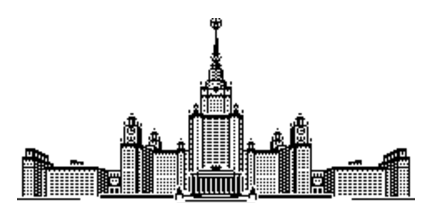
\includegraphics[width=0.5\textwidth]{msu.eps}\\
    {\scshape Московский государственный университет имени М.\,В. Ломоносова}\\
    Факультет вычислительной математики и кибернетики\\
    \vfill
    {\LARGE Лекции по курсу}\\
    \vspace{0.55cm}
    {\Huge\bfseries Численные методы}\\
\end{center}
%
\vspace{1cm}
%
\begin{center}
    \textit{Лекторы}\\
    А.\,В. Гулин,
    Н.\,И. Ионкин\\
\end{center}

%
\vfill
%
\begin{center}
    Москва, 2013
\end{center}
%
\newpage

\addtocontents{toc}{\protect\thispagestyle{empty}}
\tableofcontents
%
\newpage
%
\phantomsection
\pagestyle{empty}
%
\chapter*{Предисловие от авторов}
%
\addcontentsline{toc}{chapter}{Предисловие от авторов}
\vspace{0.5cm}
Читателю предлагается курс лекций по численным методам, который авторы
читали в течение десятков лет студентам III~-- IV курсов программистских
кафедр факультета ВМК МГУ. Безусловно, программа и содержание курса
неоднократно менялись как в связи с обновлением курса, так и в связи
с преобразованиями учебных планов, происходившими в разные годы на
факультете. Здесь представлен вариант курса, читаемого в последние годы.

Решение издать курс лекций обусловлено постоянными из года в год просьбами
студентов, слушающих этот курс, оформить лекции в печатной и электронной
версиях.

Данный курс лекций ориентирован на студентов, основной специализацией которых
не является разработка и обоснование численных методов решения прикладных
задач.

Тем не менее, одной из главных задач этого курса является обретение
студентами навыка ориентирования в области численных методов, умения применять
к решению прикладных задач основополагающие приемы построения и исследования
вычислительных алгоритмов.

Авторы считают своим приятным долгом выразить благодарность студентам кафедры
АСВК В.\,С. Алтухову, М.\,А. Казачук, М.\,В. Коростелевой, С.\,В. Селецкому,
А.\,В. Фролову, и В.\,И. Шахуро, которые с энтузиазмом и творчески записали
и оформили лекции курса.

\begin{flushright}
    \textit{Заслуженный профессор МГУ, А.\,В. Гулин}\\
    \textit{Заслуженный преподаватель МГУ, доцент Н.\,И. Ионкин}\\
\end{flushright}

%
\newpage
\phantomsection
\pagestyle{empty}
%
\chapter*{Введение}
%
\addcontentsline{toc}{chapter}{Введение}
\vspace{0.5cm}
%%%%%%%%%%%%%%%%%%%%%%%%%%%%%%%%%%%%%%%%%%%%%%%%%%%%%%%%%%%%%%%%%%%%%%%%%%%%%%%
\ifx false
Настоящее пособие представляет собой конспект курса лекций по численным
методам, читаемого студентам третьего курса факультета вычислительной
математики и кибернетики МГУ им. М.В.Ломоносова.

Численные методы~"--- это методы приближенного решения математических задач,
сводящиеся к выполнению конечного числа элементарных операций над входными
данными.  В современном мире численные методы играют огромную роль не только
как способ проведения и оптимизации расчетов для конкретных прикладных задач,
но и как часть системы научного познания; они позволяют расширить наши представления
об окружающем мире. Наглядно демонстрирует данный факт принцип колеса Самарского,
использующийся при изучении объектов и явлений окружающего мира математическими
методами.
\fi
%%%%%%%%%%%%%%%%%%%%%%%%%%%%%%%%%%%%%%%%%%%%%%%%%%%%%%%%%%%%%%%%%%%%%%%%%%%%%%%
Предмет численных методов, если его понимать не как учебный курс, а как отрасль
науки, весьма обширен и неоднороден. В очень общих чертах его можно охарактеризовать
как совокупность приемов и методов, позволяющих с помощью компьютера решать те или
иные задачи, уже получившие математическую формулировку.

Предполагается, что читатель знаком с некоторыми численными методами. Так, в курсах
анализа и алгебры рассматривались приближенные методы вычисления определенных
интегралов, нахождения корней алгебраических уравнений, решения систем линейных
алгебраических уравнений. Из курса <<Введение в численные методы>> читатель
получил представление о приближенном решении обыкновенных дифференциальных уравнений
с помощью метода конечных разностей.

Нетрудно видеть, что общим для всех перечисленных методов является построение и
обоснование алгоритма, позволяющего дать решение исходной задачи в виде числа или
таблицы чисел.

Обычно процесс решения прикладной задачи складывается из нескольких крупных этапов,
образующих, как иногда говорят, <<колесо Самарского>> (А.\,А. Самарский~"--- один из
крупнейших математиков XX века в области численных методов решения актуальных
прикладных задач).
%
\begin{center}
    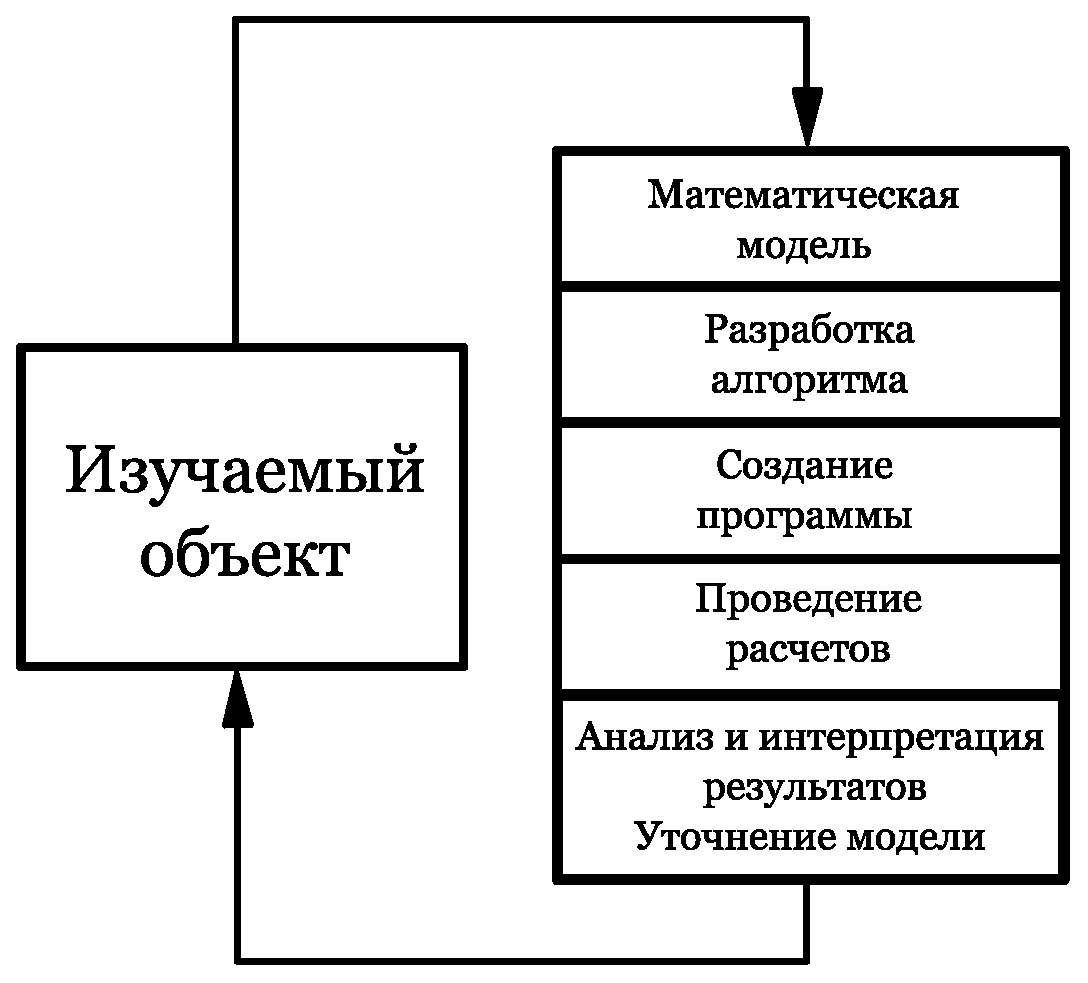
\includegraphics[width=0.5\textwidth]{circle.eps}\\
\end{center}
%

Принцип колеса Самарского заключен в следующем: сначала по изучаемому
объекту строится его математическая модель, которая отражает существенные в
данной задаче свойства изучаемого объекта. Затем для построенной модели
предлагается алгоритм решения поставленной задачи и приводится его формальное
обоснование. По предложенному алгоритму создается программа для выполнения
численных расчетов на ЭВМ, после чего уже производятся сами расчеты, анализ
результатов выполнения алгоритма, их интерпретация и, возможно, уточнение
модели. Получение новых данных расширяет существующие знания об изучаемом
объекте, появляются новые задачи, и колесо Самарского замыкается.

В рамках данного курса численных методов рассматривается этап разработки
алгоритма для некоторых классов математических моделей. Мы предполагаем, что
каждая из рассматриваемых нами математических моделей построена корректно
(рассмотрение решения задач для некорректных математических моделей выходит
за рамки нашего курса).

Данный курс разделен на пять глав. В главе I рассматриваются прямые и
итерационные численные методы решения систем линейных алгебраических уравнений,
а также исследуются итерационные методы решения частичной и полной проблем
собственных значений. В главе II представлены методы интерполирования и
приближения функций. В главе III описаны методы решения нелинейных уравнений
и систем нелинейных уравнений.
На практике часто встречается задача численного решения дифференциальных уравнений,
которой посвящены главы IV и V. Так, в главе IV приводятся описание и анализ
разностных методов решения задач математической физики. А в заключительной, пятой,
главе рассматриваются методы численного решения задач Коши для обыкновенных
дифференциальных уравнений.
\\~\\~\\
\ifx false
Запись и верстку лекций выполнили студенты кафедры {\scshape асвк}\\
    Виктор Алтухов,
    Мария Казачук,
    Мария Коростелева,\\
    Станислав Селецкий,
    Алексей Фролов,
    Влад Шахуро.
\\~\\
\fi
Свежую версию лекций можно скачать на~странице
\href{https://github.com/shahurik/num-cmc}{github.com/shahurik/num-cmc}.\\
Кроме того, по всем вопросам можно написать по адресу
\href{mailto:num-cmc@ya.ru}{num-cmc@ya.ru}.


\newpage
\phantomsection
\chapter*{Список обозначений}
\addcontentsline{toc}{chapter}{Список обозначений}
%
\noindent
$\mathbb{N}$~"--- множество натуральных чисел: \{1,2, \ldots\};\\
$\mathbb{Z}$~"--- множество целых чисел;\\
$\mathbb{Z}_+$~"--- множество целых неотрицательных чисел;\\
$\mathbb{R}$~"--- множество вещественных чисел;\\
$\mathbb{R}_+$~"--- множество вещественных неотрицательных чисел;\\
$\mathbb{C}$~"--- множество комплексных чисел;\\
$f(x)=\bigO{g(x)}$~"--- функция $f$ асимптотически ограничена сверху
функцией $g$ (с точностью до постоянного множителя);\\
$\vfunc{f}(x)$~"--- вектор-функция;\\
%$\ceil{x}$~"--- округление до ближайшего целого числа в большую сторону;\\
%$\lfloor{x}\rfloor$~"--- округление до ближайшего целого числа в меньшую сторону.\\
$[x]$~"--- целая часть числа $x$.\\

\noindent
В следующих обозначениях $m$ и $n$~"--- натуральные числа.\\
$A~(m\times n)$~"--- вещественная (если не сказано иное)
матрица $A$, содержащая $m$ строк и $n$ столбцов;\\
$\mathbb{R}^{m\times n}$~"--- множество всех матриц
размера $m\times n$ над полем вещественных чисел;\\
$\mathbb{C}^{m\times n}$~"--- множество всех матриц
размера $m\times n$ над полем комплексных чисел.\\

\noindent
Размер следующих матриц и вектора определяется по контексту.\\
$\theta$~"--- нулевой вектор-столбец;\\
$E$~"--- единичная матрица;\\
$\mathbf{0}$~"--- нулевая матрица;\\

\noindent
$\Box$~"--- конец доказательства;\\
$\delta_{ij}$~"--- символ Кронекера:
%
$$
    \delta_{ij}=
    %
    \begin{cases}
        1 & \textup{при}~~ i=j,\\
        0 & \textup{при}~~ i \ne j.
    \end{cases}
    %
$$
%

\newpage
\pagestyle{fancy}
%
%
%
\chapter{Численные методы линейной алгебры}
%
%
%
\section{Введение}
%
%
\paragraph{Решение систем линейных уравнений}
%
Рассмотрим матричное уравнение вида
%
\begin{equation}
    \label{eq:linear-system}
    %
    Ax = f,
\end{equation}
%
где $|A| \ne 0, ~A~(m \times m),~
x = (x_1, x_2, \ldots, x_m)^T,~
f = (f_1, f_2, \ldots, f_m)^T$.
\\
Так как матрица $A$ невырождена, то решение системы~\eqref{eq:linear-system}
существует и единственно. Существуют две группы методов решения СЛАУ:
%
\begin{enumerate}
    \item Прямые методы (методы Гаусса, Крамера, Холецкого и другие),
    позволяющие за конечное количество действий получить решение задачи.
    Эффективность методов этой группы оценивается по необходимому количеству
    умножений и делений. Несмотря на то, что эти методы часто называют точными,
    прямые методы таковыми не являются из-за ошибок округления при вычислении.

    \item Итерационные методы (методы Якоби, Зейделя, Самарского и другие),
    в которых задается начальное приближение $x^0$ и итерационный процесс,
    по которому строится ${x^n}$~"--- последовательность приближений,
    такая, что
    $\norm{x - x^n} < \varepsilon$
    ($\varepsilon > 0$~"--- точность приближения).

    Эффективность итерационного метода определяется числом итераций
    $n_0 = n_0(\varepsilon)$, необходимых для получения решения
    с~заданной точностью $\varepsilon$.
\end{enumerate}
%
%
\paragraph{Поиск собственных значений матрицы}
%
Задача нахождения собственных значений матрицы $A~(m \times m)$
состоит в решении уравнения
%
\begin{equation}
    Ax = \lambda x,~x \ne \theta.
\end{equation}
%
Здесь $\lambda$~"--- собственное значение, $x$~"--- собственный вектор.
Собственные значения находятся из уравнения $|A - \lambda E| = 0$,
которое в общем случае представляет из себя многочлен степени~$n$.
Однако, как было доказано Абелем и Галуа, при $n \geqslant 5$
данное уравнение не~имеет общего решения в радикалах.
Таким образом, в общем виде задачу можно решить только вычислительными методами.

\newpage
\noindent
Рассматривают две проблемы поиска собственных значений:
%
\begin{enumerate}
    \item Частичная проблема собственных значений~"---
    нахождение отдельных собственных значений (например, максимального и
    минимального по модулю).

    \item Полная проблема собственных значений (для решения обычно используется
    метод $QR$--разложения матрицы $A$)~"--- нахождение спектра
    (всех собственных значений) матрицы.
\end{enumerate}
%
%
\paragraph{Нахождение обратной матрицы}
%
%
\begin{definition}
    Матрица $A^{-1}$ называется обратной к матрице $A$, если она удовлетворяет
    равенствам
    %
    $$
        AA^{-1} = A^{-1}A=E.
    $$
    %
\end{definition}
%

Как мы помним из курса линейной алгебры, если нам известна матрица,
обратная к~матрице $A$, например, в задаче поиска решения системы линейных
уравнений~\eqref{eq:linear-system}, то~решение находится очень просто:
$x=A^{-1}f$.
В дальнейшем мы будем активно использовать понятие обратной матрицы не~только
в~контексте прямого поиска решения, но и при~исследовании на~сходимость
численных методов нахождения решений различных задач и оценке
скорости их~сходимости.
%
\section{Связь метода Гаусса с факторизацией матрицы}
%
Рассмотрим матричное уравнение вида
%
\begin{equation}
    \label{eq:linear-system-2}
    %
    Ax = f,
\end{equation}
%
где $|A| \ne 0, ~A~(m \times m),~
x = (x_1, x_2, \ldots, x_m)^T,~
f = (f_1, f_2, \ldots, f_m)^T$. Матрица $A$, вообще говоря, может быть матрицей
с~комплексными элементами.

Рассмотрим факторизацию (разложение в произведение) матрицы $A~(m \times m)$
%
\begin{equation}
    \label{eq:A-factor}
    %
    A = B \cdot C,
\end{equation}
%
где $B$~"--- нижнетреугольная матрица, а $C$~"--- верхнетреугольная матрица
с~единицами на~главной диагонали:
%
$$
    B =
    \begin{pmatrix}
        b_{11} & 0      & \cdots & 0      \\
        b_{21} & b_{22} & \cdots & 0      \\
        \vdots & \vdots & \ddots & \vdots \\
        b_{m1} & b_{m2} & \cdots & b_{mm}
    \end{pmatrix},
    ~~~C =
    \begin{pmatrix}
        1      & c_{12} & \cdots & c_{1m} \\
        0      & 1      & \cdots & c_{2m} \\
        \vdots & \vdots & \ddots & \vdots \\
        0      & 0      & \cdots & 1
    \end{pmatrix}.
$$
%
Ясно, что не любую матрицу $A$ можно представить в виде~\eqref{eq:A-factor}.
В дальнейшем мы покажем, что нахождение элементов матриц $B$ и $C$
возможно при~определенном ограничении на матрицу $A$.
Запишем определение элемента матрицы $A$ через произведение $i$-ой строки
матрицы~$B$ и $j$-ого столбца матрицы~$C$:
%
$$
    a_{ij} = \sum\limits_{l=1}^m b_{il}c_{lj}.
$$
%
Выделим $j$-ое слагаемое:
%
$$
    a_{ij} = \sum\limits_{l=1}^{j-1}b_{il}c_{lj} + b_{ij}c_{jj} +
             \sum\limits_{l=j+1}^m b_{il}c_{lj}.
$$
%
Учитывая структуру матрицы $C$ $(c_{lj} = 0, l > j, c_{jj} = 1)$, получим
%
\begin{equation}
    \label{eq:b-ij}
    %
    b_{ij} = a_{ij} - \sum\limits_{l=1}^{j-1}b_{il}c_{lj},~~~i \geqslant j.
\end{equation}
%
Аналогично, в определении элемента матрицы $A$ выделим $i$-ое слагаемое:
%
$$
    a_{ij} = \sum\limits_{l=1}^{i-1}b_{il}c_{lj} + b_{ii}c_{ij} +
             \sum\limits_{l=i+1}^m b_{il}c_{lj}.
$$
%
Исходя из вида матрицы $B$ $(b_{il} = 0, l > i)$, получим
%
$$
    b_{ii}c_{ij} = a_{ij} - \sum\limits_{l=1}^{i-1}b_{il}c_{lj}.
$$
%
Предполагая, что $b_{ii} \ne 0$, поделим левую и правую части уравнения
на~$b_{ii}$:
%
\begin{equation}
    \label{eq:c-ij}
    %
    c_{ij} = \frac{a_{ij} - \sum\limits_{l=1}^{i-1}b_{il}c_{lj}}{b_{ii}},
    ~~~i < j.
\end{equation}
%
Несмотря на то, что уравнения~\eqref{eq:b-ij} и~\eqref{eq:c-ij}
образуют нелинейную систему уравнений, элементы матриц $B$ и $C$
можно вычислить по явным формулам. Приведем алгоритм нахождения элементов
матриц $B$ и $C$.
%
\begin{enumerate}
    \item $b_{11} = a_{11}$. Найдем элементы $1$-й строки матрицы $C$:
    %
    $$
        c_{1j} = \frac{a_{1j}}{b_{11}},~~~j=\overline{2,m}.
    $$
    %

    \item Рассмотрим элементы 1-ого столбца матрицы $B$:
    %
    $$
        b_{i1} = a_{i1},~~~i=\overline{2,m}.
    $$
    %

    \item $b_{22} = a_{22} - b_{21}c_{12}$. Далее, аналогично 1-ому шагу,
    найдем элементы $2$-ой строки матрицы~$C$:
    %
    $$
        c_{2j} = \frac{a_{2j}-b_{21}c_{1j}}{b_{22}},~~~j=\overline{3,m}.
    $$
    %

    \item Вычислим элементы 2-ого столбца матрицы $B$ аналогично 2-ому шагу:
    %
    $$
        b_{i2} = a_{i2} - b_{i1}c_{12},~~~i=\overline{3,m}.
    $$
    %

    \item Повторяя последовательно шаги алгоритма для столбцов матрицы $B$
    и строк матрицы $C$, найдем все элементы матриц $B$ и $C$.

\end{enumerate}
%
%
\begin{statement}
    Пусть все угловые миноры матрицы $A$ отличны от~нуля. Тогда представление
    матрицы $A$ в~виде~\eqref{eq:A-factor} существует и единственно.
\end{statement}
%
%
\begin{proof}
    Обозначим $|A_1| = a_{11} \ne 0$,
    $
    A_2 =
    %
    \begin{vmatrix}
        a_{11} & a_{12} \\
        a_{21} & a_{22}
    \end{vmatrix}
    %
    $,
    $\ldots,$
    $
    A_i =
        %
        \begin{vmatrix}
            a_{11} & \ldots & a_{1i} \\
            \vdots & \ddots & \vdots \\
            a_{i1} & \ldots & a_{ii}
        \end{vmatrix},
        %
    ~i~=~\overline{1,m}.
    $
    Поскольку $|A_i| \ne 0$, введем для определенности $|A_0| = 1$.
    %
    $$
    A_i = B_i \cdot C_i,~~~i=\overline{1,m}.
    $$
    %
    %
    Подсчитаем значение определителя матрицы $A_i$, приняв во внимание вид матриц $C_i$ и $B_i$
    и равенство $|C_i| = 1$:
    %
    %
    $$
        |A_i| = |B_i||C_i| =
            \underbrace{b_{11}b_{22}\cdot\ldots\cdot b_{i-1,i-1}}_{|A_{i-1}|}
            b_{ii},
    $$
    %
    %
    $$
        b_{ii} = \frac{|A_i|}{|A_{i-1}|} \ne 0,~~~ i = \overline{1,m}.
    $$
    %
    Подставив $b_{ii}$ в формулы~\eqref{eq:b-ij} и~\eqref{eq:c-ij},
    получим факторизацию матрицы $A$. Следовательно, факторизация матрицы $A$
    в~виде~\eqref{eq:A-factor} существует и определяется единственным образом.
\end{proof}
%
%
\begin{problem}
    Показать, что для вычисления элементов матриц $B$ и $C$ по формулам
   ~\eqref{eq:b-ij} и~\eqref{eq:c-ij} требуется $\frac{m^3-m}{3}$
    умножений и делений.
\end{problem}
%
%
\begin{solution}
    Оценим необходимое количество операций для вычисления элементов $b_{ij}$
    по формуле~\eqref{eq:b-ij}. Для вычисления фиксированного $b_{ij}$
    потребуется $(j-1)$ умножение.
    Зафиксировав $i$ и учитывая, что $i \geqslant j$, получим
    %
    $$
        \sum_{j=1}^i(j-1) = \frac{i(i-1)}{2}.
    $$
    %
    Далее, варьируя $i$ от $1$ до $m$, получим
    %
    $$
        \sum_{i=1}^m \frac{i(i-1)}{2} = \frac{1}{2}\left(\sum_{i=1}^m i^2 -
            \sum_{i=1}^m i \right) = \frac{1}{2}\left(\frac{m(m+1)(2m+1)}{6} -
                \frac{m(m+1)}{2}\right) = \frac{m(m-1)(m+1)}{6}.
    $$
    %

    Оценим необходимое количество операций для вычисления элементов $c_{ij}$
    по формуле~\eqref{eq:c-ij}. Для вычисления фиксированного $c_{ij}$
    потребуется $(i-1)$ умножение и одно деление.
    При фиксированном $j$ получим
    %
    $$
        \sum_{i=1}^{j-1}i = \frac{j(j-1)}{2}.
    $$
    %
    Далее, варьируя $j$ от $1$ до $m$, получим аналогичную формулу:
    %
    $$
        \sum_{j=1}^m \frac{j(j-1)}{2} = \frac{m(m-1)(m+1)}{6}.
    $$
    %
    Сложив необходимое количество операций для вычисления $b_{ij}$ и $c_{ij}$,
    получим искомый результат:
    %
    $$
        \frac{m(m-1)(m+1)}{6} + \frac{m(m-1)(m+1)}{6} = \frac{m^3-m}{3}.
    $$
    %
\end{solution}
%
%
\begin{note*}
    Классическим методом решения СЛАУ вида~\eqref{eq:linear-system-2}
    является метод Гаусса. Кратко вспомним, в чем он заключается:
    %
    \begin{enumerate}
        %
        \item Прямой ход. С помощью элементарных преобразований матрица $[A|f]$,
        получаемая приписыванием к матрице $A$ вектор-столбца $f$ правых частей
        системы уравнений~\eqref{eq:linear-system-2},
        приводится к матрице $[A'|f']$, где $A'$~"--- верхнетреугольная
        матрица с~единицами на главной диагонали:
        %
        $$
            [A|f] \rightarrow \ldots \rightarrow [A'|f'].
        $$
        %
        %
        На этом этапе мы получили новую СЛАУ
        %
        \begin{equation}
            \label{A'-lin-system}
            %
            A'y=f',
        \end{equation}
        %
        эквивалентную данной: ее решение совпадает с решением исходной задачи.
        %
        \item Обратный ход метода Гаусса. Последовательно, начиная с последнего
        уравнения\linebreak СЛАУ~\eqref{A'-lin-system} и поднимаясь к первому,
        по~явным формулам вычисляются все компоненты решения системы.
        %
    \end{enumerate}
    %
    Число действий, необходимое для преобразований матрицы в~прямом ходе метода Гаусса
    равно $\frac{m^3 - m}{3}$. Подробный подсчет числа действий можно найти,
    например, в~\cite{KostFav}. Заметим, что матрица $A'$, к которой приводится матрица $A$
    в~прямом ходе метода Гаусса, в~точности совпадает с матрицей $C$, полученной
    в~результате факторизации матрицы $A$ в виде~\eqref{eq:A-factor}.
    Таким образом факторизация матрицы $A$ в виде~\eqref{eq:A-factor}
    требует такое же число действий, что и сведение матрицы $A$ к $A'$ в прямом ходе
    метода Гаусса.
\end{note*}
%

В матричном уравнении~\eqref{eq:linear-system-2} подставим $A=BC$: $BCx=f$,
обозначим $Cx=y$
и получим две системы уравнений с~треугольными матрицами:
%
\begin{numcases}{}
    \label{eq:y-system}
    %
    By=f  & \\
    %
    \label{eq:x-system}
    %
    Cx=y, & $y=(y_1,\ldots,y_m)^T$.
\end{numcases}
%
Запишем $i$-ое уравнение системы~\eqref{eq:y-system}:
%
$$
    b_{i1}y_1+b_{i2}y_2+\ldots+b_{ii}y_i=f_i,~~~i=\overline{1,m}.
$$
%
Предполагая, что $b_{ii} \ne 0$, получим
%
$$
    y_i = \frac{f_i - \sum\limits_{l=1}^{i-1}b_{il}y_l}{b_{ii}}.
$$
%
Для вычисления $y_i$ требуется $(i-1)$ умножение и $1$ деление~"--- всего
$i$ операций. Учитывая, что $i$ изменяется от $1$ до $m$, получим, что
для~решения системы~\eqref{eq:y-system} требуется
$
1+2+\ldots+m=\frac{m(m+1)}{2}
$
операций.
%
\begin{note}
    На вычисление новых правых частей, т.е. вектора $f'$, в~методе Гаусса
    уходит $\frac{m(m+1)}{2}$ действий.
    Как мы можем видеть, это число совпадает с количеством операций,
    необходимых для вычисления вектора y при решении системы~\eqref{eq:y-system}.
\end{note}
%
Аналогично, запишем $i$-ое уравнение системы~\eqref{eq:x-system}:
%
$$
    x_i + c_{i,i+1}x_{i+1} + \ldots + c_{im}x_m = y_i,
$$
%
%
$$
    x_i = y_i - \sum\limits_{l=i+1}^{m}c_{il}x_l,~~~i=\overline{1,m}.
$$
%
Для вычисления $x_i$ требуется $(m-i)$ умножений. Изменяя $i$ от $1$ до $m$,
получим, что для решения системы~\eqref{eq:x-system} требуется
$
(m-1)+(m-2)+\ldots+2+1=\frac{m(m-1)}{2}
$
умножений.
%
\begin{note}
    Число операций, затрачиваемых на выполнение обратного хода метода Гаусса, равно
    $\frac{m(m-1)}{2}$, что совпадает с числом действий, требуемых для решения
    системы~\eqref{eq:x-system}.
\end{note}
%

В итоге получим, что для решения систем~\eqref{eq:y-system} и
\eqref{eq:x-system} требуется
$
\frac{m(m-1)}{2}+\frac{m(m+1)}{2}=m^2
$
операций. Тогда все решение системы~\eqref{eq:linear-system-2} с использованием
факторизации матриц требует
$
\frac{m^3-m}{3}+m^2=\frac{m^3+3m^2-m}{3}
$
операций, что равно общему числу операций, необходимых для решения
этой же системы методом Гаусса. Таким образом, решение системы
\eqref{eq:linear-system-2}
методом Гаусса эквивалентно по числу операций факторизации матрицы и
решению двух систем уравнений.
%
\begin{note}
    Возникает вопрос о необходимости решения СЛАУ~\eqref{eq:linear-system-2}
    именно с~использованием факторизации вместо классического метода Гаусса.
    Выигрыш по числу операций обусловлен особенностями задач, встречающихся
    на~практике: как правило, решаются целые серии задач с~одной и той же
    матрицей $A$, которая описывает математическую модель изучаемого
    объекта или процесса, и с различными правыми частями $f$, которые
    соответствуют изменяющимся входным условиям.
     Таким образом, можно один раз факторизовать матрицу
    $A$, а затем для нахождения решения каждой задачи решать лишь СЛАУ
    вида~\eqref{eq:y-system} и~\eqref{eq:x-system} для каждого наблюдения.
\end{note}
%
%
\section{Обращение матрицы методом Гаусса-Жордана}
%
Рассмотрим задачу обращения (поиска обратной матрицы) невырожденной матрицы
$A~(m \times m)$.
%
%\begin{definition}
%    Матрица $A^{-1}$ называется {\it обратной} к матрице $A$,
%    если она удовлетворяет равенствам
    %
%    $$
%        AA^{-1} = A^{-1}A=E.
%    $$
    %
%\end{definition}
%
Согласно критерию обратимости матрицы, для невырожденной матрицы всегда
существует обратная. Введем обозначение:
$
A^{-1}=X=(x_{ij}),~i,j = \overline{1,m}.
$
С учетом этого задача обращения матрицы состоит в решении системы
%
\begin{equation}
    \label{eq:AX-system}
    %
    AX=E,
\end{equation}
%
где $A~(m \times m)$,~$|A| \ne 0$, или, если записать поэлементно:
%
\begin{equation}
    \label{eq:AX-sum-system}
    %
    \sum\limits_{l=1}^m a_{il}x_{lj}=\delta_{ij}.
\end{equation}
%

Можно приступить к решению последней системы методом Гаусса без~учета
структуры матрицы коэффициентов.
Эта система имеет $m^2$ неизвестных переменных, число требуемых для решения
операций будет
пропорционально $m^6$. Покажем, что существует способ обращения матрицы,
требующий ровно $m^3$ операций. Более того, в случае, если матрица $A$ имеет
специальную структуру (например, если матрица $A$~"--- блочная или
трехдиагональная), число операций уменьшится.

Сведем уравнение~\eqref{eq:AX-sum-system} к решению $m$ систем линейных
уравнений с матрицей $A$. Для этого введем вектор-столбец матрицы $X$:
$
X^{(j)} = (x_{1j}, x_{2j}, \ldots, x_{mj})^T
$
и вектор-столбец правой части
$
\delta^{(j)} = (0, 0, \ldots, 0, 1, 0, \ldots , 0)^T
$
с единицей на $j$-ой позиции. Теперь можем записать матричное уравнение
\eqref{eq:AX-system} в виде $m$ систем:
%
\begin{equation}
    \label{eq:AX-j-system}
    %
    AX^{(j)}=\delta^{(j)},~~~j = \overline{1,m}.
\end{equation}
%
Факторизуем матрицу $A$ в виде
%
\begin{equation}
    \label{eq:A-BC-system}
    %
    A = B \cdot C.
\end{equation}
%
Для этого требуется $\frac{m^3-m}{3}$ умножений и делений.
Получаем две системы линейных уравнений:
%
\begin{numcases}{}
    \label{eq:yd-system}
    %
    By^{(j)}=\delta^{(j)} & \\
    %
    \label{eq:xy-system}
    %
    Cx^{(j)}=y^{(j)}. &
\end{numcases}
%
При фиксированном $j$ решение систем~\eqref{eq:yd-system} и~\eqref{eq:xy-system}
требует число действий, ~равное $m^2$.
Для~решения $m$ ~таких ~систем ~при ~~$j=\overline{1,m}$ ~~потребуется ~$m^3$
~действий. ~~Значит, ~в ~целом для~обращения матрицы $A$ необходимо~
$
~m^3+\frac{m^3-m}{3} \sim \frac{4}{3}m^3
$
операций. Покажем теперь, что это число операций можно уменьшить.
Рассмотрим систему уравнений~\eqref{eq:yd-system}:
%
\begin{alignat*}{2}
    b_{11}y_1^{(j)}=0 ~~~&
        \Rightarrow ~~~& y_{1}^{(j)}=0,\\
    %
    b_{21}y_1^{(j)}+b_{22}y_2^{(j)}=0 ~~~&
        \Rightarrow ~~~& y_{2}^{(j)}=0,\\
    %
    b_{31}y_1^{(j)}+b_{32}y_2^{(j)}+b_{33}y_3^{(j)}=0 ~~~&
        \Rightarrow ~~~& y_{3}^{(j)}=0,\\
    %
    \ldots &\\
    %
    b_{j-1,1}y_1^{(j)} + \ldots + b_{j-1, j-1}y_{j-1}^{(j)}=0 ~~~&
        \Rightarrow ~~~& y_{j-1}^{(j)}=0.
    %
\end{alignat*}
%
Рассмотрим $j$-ое уравнение: $b_{jj}y_j^{(j)}=1$.
Предполагая, что $b_{jj}\neq0$, получим:
%
\begin{equation}
    \label{eq:ast-equation}
    %
    y_j^{(j)}=\frac{1}{b_{jj}}.
\end{equation}
%
Запишем уравнения системы при $i > j$
%
\begin{equation}
    b_{ij}y_{j}^{(j)}+b_{i,j+1}y_{j+1}^{(j)}+\ldots+b_{ii}y_i^{(j)}=0,
        ~~~i = \overline{(j+1),m},
\end{equation}
%
и выразим из~них $y_i^{(j)}$:
%
\begin{equation}
    \label{eq:spec-yi-system}
    %
    y_i^{(j)}=\frac{-\sum\limits_{l=j}^{i-1} b_{il}y_l^{(j)}}{b_{ii}},
        ~~~i = \overline{(j+1),m}.
\end{equation}
%
Перейдем к подсчету числа операций, необходимых для решения систем уравнений
\eqref{eq:yd-system}~и~\eqref{eq:xy-system}.
При фиксированных $i$ и $j$ в формуле~\eqref{eq:spec-yi-system} получаем
$(i-j)$ умножений и одно деление и в~уравнении~\eqref{eq:ast-equation} одно деление.
Варьируя индекс $i$ от $1$ до $m$, при фиксированном $j$ получаем
%
$$
    (m-j)+(m-j-1)+\ldots+1=\frac{(m-j)(m-j+1)}{2}
$$
%
умножений и $(m-j+1)$ делений. Таким образом, число действий, необходимое
для решения одной системы~\eqref{eq:yd-system} равно
%
$$
    \frac{(m-j)(m-j+1)}{2}+\frac{2(m-j+1)}{2}=\frac{(m-j+1)(m-j+2)}{2}.
$$
%
Общее число действий, необходимое
для~решения всех систем~\eqref{eq:yd-system} равно
%
\begin{equation}
    \label{eq:all-actions}\sum\limits_{j=1}^{m} \frac{(m-j+1)(m-j+2)}{2}.
\end{equation}
%
%
\begin{problem}
    Показать, что сумма~\eqref{eq:all-actions} равна $\frac{m(m+1)(m+2)}{6}$.
\end{problem}
%
%
\begin{solution}
    Сделаем замену $k=m-j+1$ в формуле~\eqref{eq:all-actions}:
    %
    $$
        \sum\limits_{j=1}^{m} \frac{(m-j+1)(m-j+2)}{2} =
            \sum_{k=1}^m \frac{k(k+1)}{2}.
    $$
    %
    Преобразовав полученное выражение, получим искомый результат:
    %
    $$
        \frac{1}{2}\left(\sum_{k=1}^m k^2 + \sum_{k=1}^m k\right)=
            \frac{1}{2}\left(\frac{m(m+1)(2m+1)}{6} + \frac{m(m+1)}{2}\right) =
                \frac{m(m+1)(m+2)}{6}.
    $$
    %
\end{solution}
%
\noindent
Аналогично получаем, что число операций для~решения всех систем вида
\eqref{eq:xy-system}
равно $\frac{m^2(m-1)}{2}$. Просуммируем число операций для факторизации
исходной матрицы и для решения систем~\eqref{eq:yd-system} и
\eqref{eq:xy-system} при $j=\overline{1,m}$:
%
$$
    \frac{m^3-m}{3}+\frac{m(m+1)(m+2)}{6}+\frac{m^2(m-1)}{2}=m^3.
$$
%

Описанный выше метод обращения произвольной невырожденной матрицы называется
методом Гаусса-Жордана. Отметим, что он является самым эффективным
методом обращения невырожденных матриц произвольного вида.
%
\section{Метод квадратного корня}
%
%
\begin{definition}
    Квадратная матрица $A$ называется эрмитовой (самосопряженной),
    если $A=A^*$ (ее элементы связаны соотношением $a_{ij} = \overline{a_{ji}}$).
\end{definition}
%
\noindent
Рассмотрим задачу
%
\begin{equation}
    \label{eq:main-problem}
    %
    Ax = f,
\end{equation}
%
где
$A\in\mathbb{C}^{m \times m},$
$
A = A^*, ~|A| \ne 0, ~
x = (x_1, x_2, \ldots, x_m)^T,~
f = (f_1, f_2, \ldots, f_m)^T,
$
и один из~прямых методов ее решения~"--- метод квадратного корня (метод Холецкого).

Заметим, что хотя класс эрмитовых матриц с точки зрения линейной алгебры
достаточно узок, на практике часто возникают модели, описываемые именно
этим классом матриц. Поэтому с практической точки зрения такое ограничение
на~систему~\eqref{eq:main-problem} вполне допустимо.
Факторизуем эрмитову матрицу $A$ в~виде
%
\begin{equation}
    \label{eq:sds-equation}
    %
    A = S^{\ast}DS,
\end{equation}
%
где матрица $S$~"--- верхнетреугольная матрица с положительными элементами
на~главной диагонали, а $D$~"--- диагональная матрица со значениями
$\pm 1$ на главной диагонали:
%
$$
    S =
    %
    \begin{pmatrix}
        s_{11} & s_{12} & \cdots & s_{1m}  \\
        0      & s_{22} & \cdots & s_{2m}  \\
        \vdots & \vdots & \ddots & \vdots  \\
        0      & 0      & \cdots & s_{mm}
    \end{pmatrix}
    %
    , ~s_{ii} > 0,
    %
    ~~~~~D =
    %
    \begin{pmatrix}
        d_{11} & 0      & \cdots & 0       \\
        0      & d_{22} & \cdots & 0       \\
        \vdots & \vdots & \ddots & \vdots  \\
        0      & 0      & \cdots & d_{mm}
    \end{pmatrix}
    %
    , ~d_{ii} = \pm 1.
$$
%

Покажем, что факторизация~\eqref{eq:sds-equation} возможна на~примере
вещественной симметрической матрицы второго порядка:
%
$$
    A =
    \begin{pmatrix}
        a_{11} & a_{12} \\
        a_{21} & a_{22} \\
    \end{pmatrix}
    = A^{T}, ~~a_{12} = a_{21}.
$$
%
Матрицы $S$ и $D$ будем искать в виде
$$
    S =
    %
    \begin{pmatrix}
        s_{11} & s_{12} \\
        0      & s_{22} \\
    \end{pmatrix}
    %
    ,~s_{ii} > 0,~i = 1,2,
$$
%
%
$$
    S^* = S^T =
    %
    \begin{pmatrix}
        s_{11} & 0      \\
        s_{12} & s_{22} \\
    \end{pmatrix}
    %
    ,
$$
%
%
$$
    ~~~D =
    %
    \begin{pmatrix}
        d_{11} & 0      \\
        0      & d_{22} \\
    \end{pmatrix}
    %
    , ~d_{ii} = \pm 1, ~~i = 1,2.
$$
%
Найдем матрицу $DS$:
%
$$
    DS =
    %
    \begin{pmatrix}
        d_{11} & 0      \\
        0      & d_{22} \\
    \end{pmatrix}
    %
    %
    \begin{pmatrix}
        s_{11} & s_{12} \\
        0      & s_{22} \\
    \end{pmatrix}
    %
    ~=
    %
    \begin{pmatrix}
        d_{11}s_{11} & d_{11}s_{12} \\
        0            & d_{22}s_{22} \\
    \end{pmatrix}
    %
    .
$$
%
Домножим матрицу $DS$ слева на $S^T$:
%
$$
    S^{T}DS =
    %
    \begin{pmatrix}
        s_{11} & 0      \\
        s_{12} & s_{22} \\
    \end{pmatrix}
    %
    %
    \begin{pmatrix}
        d_{11}s_{11} & d_{11}s_{12} \\
        0            & d_{22}s_{22} \\
    \end{pmatrix}
    %
    ~=
    %
    \begin{pmatrix}
        d_{11}s_{11}^2   & ~d_{11}s_{11}s_{12}                  \\
        d_{11}s_{11}s_{12} & ~d_{11}s_{12}^2 + d_{22}s_{22}^2 \\
    \end{pmatrix}
    %
    .
$$
%
Приравняем элементы матриц $A$ и $S^TDS$:
%
\begin{numcases}{}
    \label{eq:first_eq}
    %
    a_{11} = d_{11}s_{11}^2\\
    %
    \label{eq:second_eq}
    %
    a_{12} = d_{11}s_{11}s_{12}\\
    %
    \label{eq:third_eq}
    %
    a_{22} = d_{11}s_{12}^2 + d_{22}s_{22}^2.
\end{numcases}
%
Из неравенства $s_{11}>0$ и из уравнения~\eqref{eq:first_eq} следует, что
%
$$
    d_{11} = \sgn a_{11},~s_{11} = \sqrt{|a_{11}|}.
$$
%
Рассмотрим уравнение~\eqref{eq:second_eq}. Заметим,
что $s_{11}d_{11} \neq 0$, и получим
%
$$
    s_{12} = \frac{a_{12}}{s_{11}d_{11}}.
$$
%
Наконец, рассмотрим уравнение~\eqref{eq:third_eq}. Получим соотношение
$
s_{22}^2d_{22} = a_{22} - d_{11}s_{12}^2,
$
правая часть которого известна. Следовательно,
%
$$
        d_{22} = \sgn(a_{22} - s_{12}^2d_{11}),
        ~s_{22} = \sqrt{|a_{22} - s_{12}^2d_{11}|}.
$$
%
Таким образом, вещественную симметрическую матрицу второго порядка можно
факторизовать в виде~\eqref{eq:sds-equation}.

Рассмотрим теперь произвольную эрмитову матрицу $A~(m \times m)$.
Запишем уравнение для элементов матрицы $DS$:
%
$$
    (DS)_{ij} = \sum\limits_{l=1}^{m} d_{il}s_{lj}, ~~~i,j = \overline{1,m}.
$$
%
Учитывая диагональную структуру матрицы $D$, получим:
%
$$
    (DS)_{ij} = d_{ii}s_{ij}.
$$
%
Домножим матрицу $DS$ слева на $S^*$:
%
$$
    a_{ij} = (S^*DS)_{ij} = \sum\limits_{l=1}^{m} (S^{\ast})_{il}d_{ll}s_{lj},
        ~~~i,j = \overline{1,m}.
$$
%
Выделим $i$-ое слагаемое из последней суммы и учтем,
что $(S^{\ast})_{ij} = \overline s_{ji}$:
%
$$
    a_{ij} = \sum\limits_{l=1}^{i-1} \overline s_{li}d_{ll}s_{lj} +
        \overline s_{ii}d_{ii}s_{ij} +
        \sum\limits_{l=i+1}^{m} \overline s_{li}d_{ll}s_{lj},
            ~~~i,j = \overline{1,m}.
$$
%
Третье слагаемое из равенства равно нулю
в~силу того, что матрица $S^{\ast}$ является нижнетреугольной:
$\overline s_{li} = 0,~l > i$. Тогда получим:
%
\begin{equation}
    \label{eq:sum_of_two-equation}
    %
    a_{ij} = \sum\limits_{l=1}^{i-1} \overline s_{li}d_{ll}s_{lj} +
        \overline s_{ii}d_{ii}s_{ij}, ~~~i,j = \overline{1,m}.
\end{equation}
%
Так как матрица $A$ эрмитова, можем рассматривать это равенство
только в случае $i \leqslant j$.
При $i = j$ получим:
%
$$
    a_{ii} = \sum\limits_{l=1}^{i-1} \overline s_{li}d_{ll}s_{li} +
        \overline s_{ii}d_{ii}s_{ii}, ~~~i = \overline{1,m}.
$$
%
Учтем, что $s_{ij}{\overline s_{ij}} = |s_{ij}|^2$:
%
$$
    a_{ii} = \sum\limits_{l=1}^{i-1} d_{ll}|s_{li}|^2 + d_{ii}|s_{ii}|^2,
        ~~~i = \overline{1,m},
$$
%
%
$$
    d_{ii}|s_{ii}|^2 =  a_{ii} - \sum\limits_{l=1}^{i-1} |s_{li}|^2d_{ll},
        ~~~i = \overline{1,m}.
$$
%
Выразим $d_{ii}$ и $s_{ii}$:
%
\begin{equation}
    \label{eq:dii-equation}
    %
    d_{ii} = \sgn (a_{ii} - \sum\limits_{l=1}^{i-1} |s_{li}|^2d_{ll}),
        ~~~i = \overline{1,m},
\end{equation}
%
%
\begin{equation}
    \label{eq:sii-equation}
    %
    s_{ii} = \sqrt{\left|a_{ii} - \sum\limits_{l=1}^{i-1} |s_{li}|^2d_{ll}\right|},
        ~~~i = \overline{1,m}.
\end{equation}
%
Рассмотрим случай $i \neq j$ ($i < j$). В уравнении
\eqref{eq:sum_of_two-equation} выделим второе слагаемое:
%
$$
    \overline s_{ii}d_{ii}s_{ij} = a_{ij} -
        \sum\limits_{l=1}^{i-1} \overline s_{li}d_{ll}s_{lj},
            ~~~i,j = \overline{1,m}.
$$
%
В силу того, что $s_{ii}$~"--- вещественные положительные числа, получим
%
$$
    s_{ii}d_{ii}s_{ij} = a_{ij} -
        \sum\limits_{l=1}^{i-1} \overline s_{li}d_{ll}s_{lj},
            ~~~i,j = \overline{1,m}.
$$
%
Так как $s_{ii}d_{ii} \neq 0$, то получим выражения
для~коэффициентов $s_{ij}$:
%
\begin{equation}
    \label{eq:sij-equation}
    %
    s_{ij} = \frac{a_{ij} -
        \sum\limits_{l=1}^{i-1} \overline s_{li}d_{ll}s_{lj}}{s_{ii}d_{ii}},
            ~~~i,j = \overline{1,m},~i<j.
\end{equation}
%
Таким образом, для вычисления элементов матриц в~разложении
\eqref{eq:sds-equation} были получены явные формулы
\eqref{eq:dii-equation}\,--\,\eqref{eq:sij-equation}.

Метод квадратного корня позволяет примерно вдвое уменьшить количество операций,
необходимых для решения системы~\eqref{eq:main-problem}, по сравнению
с~методом Гаусса~"--- до $\sim\frac{m^3}{6}$ умножений и делений и $m$ операций
извлечения квадратного корня. Однако, метод справедлив только в случае,
если матрица системы линейных уравнений эрмитова.
%
\section{Примеры и канонический вид итерационных методов решения СЛАУ}
%
Рассмотрим матричное уравнение
%
\begin{equation}
    \label{eq:linear-system2}
    %
    Ax = f,
\end{equation}
%
где
$
|A| \ne 0, ~A~(m \times m),~
x = (x_1, x_2, \ldots, x_m)^T,~
f = (f_1, f_2, \ldots, f_m)^T
$.
\\
Распишем систему~\eqref{eq:linear-system2} покоординатно:
%
\begin{equation}
    \label{eq:coords-linear-system}
    %
    \sum\limits_{j=1}^{m} a_{ij}x_j = f_i, ~~~i = \overline{1,m}.
\end{equation}
%
\\
Выделим $i$-ое слагаемое в сумме:
%
$$
    \sum\limits_{j=1}^{i-1} a_{ij}x_j + a_{ii}x_i +
        \sum\limits_{j=i+1}^{m} a_{ij}x_j= f_i, ~~~i = \overline{1,m}.
$$
%
Предположим, что элементы главной диагонали матрицы $A$ отличны от нуля:
$a_{ii} \neq 0, ~i = \overline{1,m}$. Тогда уравнение
%
\eqref{eq:coords-linear-system} разрешимо относительно $x_i$:
$$
    x_i = \frac{f_i - \sum\limits_{j=1}^{i-1} a_{ij}x_j -
        \sum\limits_{j=i+1}^{m} a_{ij}x_j}{a_{ii}}, ~~~i = \overline{1,m}.
$$
%
\\
Все итерационные методы ~основаны ~на ~построении ~последовательности ~векторов
$x^n = (x_1^n, \ldots, x_m^n)$ такой, что $x^n \rightarrow x$
при~$n \rightarrow \infty$, где $x$~"--- точное решение матричного уравнения~
\eqref{eq:linear-system2}. Вектор $x^n$ называется {\it $n$-ой итерацией метода}.

Отметим, что при выборе итерационного метода важно, чтобы метод был легко
реализуем и сходился к решению достаточно быстро.
%
\begin{definition}
    Итерационный метод называется двухслойным, если для вычисления текущей
    итерации используются только элементы текущей и предыдущей итераций.
\end{definition}
%
%
\begin{note*}
    Определенный выше итерационный метод также можно называть одношаговым.
\end{note*}
%

В этом случае для того, чтобы начать процесс построения последовательности $x^n$,
необходимо задать начальное приближение $x^0$. Далее будем предполагать,
что {\it начальное приближение уже задано}.

Рассмотрим в качестве примера два простейших из двухслойных итерационных методов:
метод Якоби и метод Зейделя.
%
\paragraph{Метод Якоби}
%
Метод Якоби является явным итерационным методом и задается уравнением
$$
    x_i^{n+1} = \frac{f_i - \sum\limits_{j=1}^{i-1} a_{ij}x_j^n -
        \sum\limits_{j=i+1}^{m} a_{ij}x_j^n}{a_{ii}},
            ~~~i = \overline{1,m}, ~n \in \mathbb{Z}_+.
$$
%
Забегая вперед, заметим, что метод Якоби является легко реализуемым,
но при этом медленно сходящимся.
%
\paragraph{Метод Зейделя}
%
Метод Зейделя, в отличие от метода Якоби, является неявным
итерационным методом и задается уравнением
%
$$
    x_i^{n+1} = \frac{f_i - \sum\limits_{j=1}^{i-1} a_{ij}x_j^{n+1} -
        \sum\limits_{j=i+1}^{m} a_{ij}x_j^n}{a_{ii}},
            ~~~i = \overline{1,m}, ~n \in \mathbb{Z}_+.
$$
%
В правой части уравнения используются
координаты $(n+1)$-ой итерации, поэтому метод Зейделя является неявным.
Но если разумно организовать вычисления, то можно найти координаты
$(n+1)$-ой итерации по явным формулам.
\\
Рассмотрим метод Зейделя при $i = 1$:
%
$$
    x_1^{n+1} = \frac{f_1 - \sum\limits_{j=2}^{m} a_{1j}x_j^n}{a_{11}},
        ~~~n \in \mathbb{Z}_+.
$$
%
Видно, что $x_1^{n+1}$ находится по явной формуле. Рассмотрим вторую координату
$(n+1)$-ой итерации:
%
$$
    x_2^{n+1} = \frac{f_2 - a_{21}x_1^{n+1} -
        \sum\limits_{j=3}^{m} a_{2j}x_j^n}{a_{22}}, ~~~n \in \mathbb{Z}_+.
$$
%
Так как координата $x_1^{n+1}$ известна, то координату $x_2^{n+1}$ можно найти
по явной формуле. Продолжая вычисления,
получим, что каждый элемент $(n+1)$-ой итерации
можно найти по~явным формулам от~уже известных элементов. Заметим, что метод
Зейделя прост в~реализации, но медленно сходится.
%
\paragraph{Каноническая запись итерационных методов}
%
Для исследования сходимости итерационных методов удобно записывать их
в~матричном виде.
Представим матрицу $A$ в виде
%
$$
    A = R_1 + D + R_2,
$$
%
где $R_1$~"--- нижнетреугольная матрица с нулевой главной диагональю,
$D$~"--- диагональная матрица, $R_2$~"--- верхнетреугольная матрица с~нулевой
 главной диагональю:
$$
    R_1 =
    %
    \begin{pmatrix}
        0      & 0      & \cdots & 0  \\
        a_{21} & 0      & \cdots & 0  \\
        \vdots & \vdots & \ddots & \vdots  \\
        a_{m1} & a_{m2} & \cdots & 0
    \end{pmatrix}
    %
    ,
    ~~~D =
    %
    \begin{pmatrix}
        a_{11} & 0      & \cdots & 0  \\
        0      & a_{22} & \cdots & 0  \\
        \vdots & \vdots & \ddots & \vdots  \\
        0      & 0      & \cdots & a_{mm}
    \end{pmatrix}
    %
    ,
    ~~~R_2 =
    %
    \begin{pmatrix}
        0      & a_{12} & \cdots & a_{1m} \\
        0      & 0      & \cdots & a_{2m} \\
        \vdots & \vdots & \ddots & \vdots \\
        0      & 0      & \cdots & 0
    \end{pmatrix}
    .
$$
%
Перепишем матричное уравнение~\eqref{eq:linear-system2} в виде
%
$$
    (R_1 + D + R_2)x = f.
$$
%
Оставим в левой части слагаемое с матрицей $D$, остальные слагаемые перенесем
в~правую часть уравнения:
%
$$
    Dx = f - R_1x - R_2x.
$$
%
Предположим, что матрица $D$ обратима ($a_{ii} \neq 0, ~i = \overline{1,m}$).
Тогда получим:
%
\begin{equation}
    \label{eq:x-matr-equation}
    %
    x = D^{-1}f - D^{-1}R_1x - D^{-1}R_2x.
\end{equation}
%
Запишем итерационные методы Якоби ({\scshape МЯ}) и Зейделя
({\scshape МЗ})
исходя из уравнения~\eqref{eq:x-matr-equation}:

%
\begin{alignat*}{2}
    ~\textup{{\scshape МЯ}}: &~~~x^{n+1} = D^{-1}f - D^{-1}R_1x^n - D^{-1}R_2x^n,
        &~~~n \in \mathbb{Z}_+,\\
    %
    ~\textup{{\scshape МЗ}}: &~~~x^{n+1} = D^{-1}f - D^{-1}R_1x^{n+1} - D^{-1}R_2x^n,
        &~~~n \in \mathbb{Z}_+.
\end{alignat*}
%
Рассмотрим эти два метода без обращения матрицы $D$:
%
\begin{alignat*}{2}
    ~\textup{{\scshape МЯ}}: &~~~ Dx^{n+1} + (R_1 + R_2)x^n = f,
        &~~~n \in \mathbb{Z}_+,\\
    %
    ~\textup{{\scshape МЗ}}: &~~~ (D + R_1)x^{n+1} + R_2x^n = f,
        &~~~n \in \mathbb{Z}_+.
\end{alignat*}
%
Перепишем эти соотношения в~виде
%
\begin{alignat}{2}
    \label{eq:jacob-matr-equation2}
    %
    ~\textup{{\scshape МЯ}}: &~~~ D(x^{n+1} - x^n) + Ax^n = f,
        &~~~n \in \mathbb{Z}_+,\\
    %
    \label{eq:seidel-matr-equation2}
    %
    ~\textup{{\scshape МЗ}}: &~~~ (D + R_1)(x^{n+1} - x^n) + Ax^n = f,
        &~~~n \in \mathbb{Z}_+.
\end{alignat}
%
Из формул~\eqref{eq:jacob-matr-equation2} и~\eqref{eq:seidel-matr-equation2}
видно, что если в каждом из методов последовательность итераций сходится,
то она сходится к решению системы~\eqref{eq:linear-system2}.

Мы видим, что один и тот же итерационный метод можно записать различными
способами. Поэтому целесообразно ввести какую-то стандартную (каноническую)
форму записи итерационных методов.
%
\begin{definition}
    Канонической формой записи двухслойного итерационного метода решения системы
   ~\eqref{eq:linear-system2} называется его запись в виде
    %
    \begin{equation}
        \label{eq:iter-process2}
        %
        B_{n+1}\frac{x^{n+1} - x^n}{\tau_{n+1}} + Ax^n = f,
    \end{equation}
    %
    где $n \in \mathbb{Z}_+$, начальное приближение $x^0$ задано,
    $\tau_{n+1}$~"--- положительное вещественное число, называемое
    итерационным параметром, $B_{n+1}$~"--- некоторая обратимая матрица.
\end{definition}
%
%
\begin{definition}
    Если в методе~\eqref{eq:iter-process2} параметр $\tau_{n+1}$ и матрица
    $B_{n+1}$ не зависят от номера итерации ($B_{n+1} = B,~\tau_{n+1} = \tau$),
    то такой метод называется стационарным, в~противном случае~"---
    нестационарным.
\end{definition}
%
%
\begin{definition}
    Если $B_{n+1} = E$, то метод~\eqref{eq:iter-process2} называется явным,
    в~противном случае~"--- неявным.
\end{definition}
%
При рассмотрении итерационных методов обычно исследуют достаточные условия,
при которых данный метод сходится, и оценивают скорость сходимости
метода.

Рассмотрим далее еще несколько примеров итерационных методов:
метод простой итерации, метод Ричардсона и попеременно-треугольный
итерационный метод. В этих методах введение параметров $\tau$ и $B$
позволяет увеличить скорость сходимости по сравнению с методами Якоби и Зейделя.
%
\paragraph{Метод простой итерации}
%
Метод простой итерации (метод релаксации) определяется итерационной схемой вида
%
\begin{equation}
    \label{eq:mpi-equation}
    \frac{x^{n+1} - x^n}{\tau} + Ax^n = f,~\tau>0,
        ~n \in \mathbb{Z}_+,~x^0 \textup{~"--- задано}.
\end{equation}
%
%
\paragraph{Метод Ричардсона}
%
Метод Ричардсона определяется итерационной схемой вида
%
\begin{equation}
    \label{eq:rich-equation}
    \frac{x^{n+1} - x^n}{\tau_{n+1}} + Ax^n = f,~\tau_{n+1}>0,
        ~n \in \mathbb{Z}_+,~x^0 \textup{~"--- задано}.
\end{equation}
%
%
\begin{note*}
    Для итерационных методов~\eqref{eq:mpi-equation} и~\eqref{eq:rich-equation}
    в случае, когда матрица $A$ является симметричной и положительно определенной,
    известен такой набор итерационных параметров (Чебышевский набор), при котором
    сходимость этих методов будет наиболее быстрая.
\end{note*}
%
%
\paragraph{Попеременно-треугольный итерационный метод (метод Самарского)}
%
Представим матрицу $A$ в виде
%
$$
    A = R_1 + R_2,
$$
%
где $R_1$~"--- нижнетреугольная матрица, $R_2$~"--- верхнетреугольная матрица:
%
$$
    R_1 =
    %
    \begin{pmatrix}
        0.5a_{11}& 0        & \cdots & 0  \\
        a_{21}   & 0.5a_{22}& \cdots & 0  \\
        \vdots   & \vdots   & \ddots & \vdots  \\
        a_{m1}   & a_{m2}   & \cdots & 0.5a_{mm}
    \end{pmatrix}
    %
    ,
    ~~~R_2 =
    %
    \begin{pmatrix}
        0.5a_{11}& a_{12}   & \cdots & a_{1m} \\
        0        & 0.5a_{22}& \cdots & a_{2m} \\
        \vdots   & \vdots   & \ddots & \vdots \\
        0        & 0        & \cdots & 0.5a_{mm}
    \end{pmatrix}
    %
    .
$$
%
Итерационная схема попеременно-треугольного метода имеет вид
%
\begin{equation}
    (E + \omega R_1)(E + \omega R_2)\frac{x^{n+1} - x^n}{\tau} + Ax^n = f,~\tau>0,
        ~n \in \mathbb{Z}_+,
\end{equation}
%
где $\tau>0,~\omega > 0$~"--- итерационные параметры, позволяющие,
вообще говоря, ускорить процесс сходимости итерационного метода.
Рассматриваемый метод формально является неявным, однако можно показать,
что $(n+1)$-ая итерация выражается с~помощью явных формул за~три шага.
Введем обозначения:
%
$$
    w^{n+1} = (E + \omega R_2)\frac{x^{n+1} - x^n}{\tau},
$$
%
%
$$
    v^{n+1} = \frac{x^{n+1} - x^n}{\tau}.
$$
%
%
\begin{definition}
    Вектор $r^n = f - Ax^n$ называется невязкой на $n$-ой итерации.
\end{definition}
%
\noindent
В нашем случае невязка $r^n$ известна. На первом шаге решим уравнение
%
$$
    (E + \omega R_1)w^{n+1} = r^n.
$$
%
Заметим, что $(E + \omega R_1)$~"--- нижнетреугольная матрица. Нахождение вектора
решения системы с~нижнетреугольной матрицей осуществляется по явным формулам,
начиная с первой компоненты вектора $w^{n+1}$.
На втором шаге аналогично решим уравнение с верхнетреугольной матрицей
$(E+\omega R_2)$:
%
$$
    (E + \omega R_2)v^{n+1} = w^{n+1}.
$$
%
На третьем шаге найдем $(n+1)$-ую итерацию по формуле
%
$$
    x^{n+1} = x^n + {\tau}v^{n+1}.
$$
%
Таким образом, несмотря на то, что метод Самарского является неявным,
его реализация не представляет никакой трудности.
%
\section{Теоремы о сходимости итерационных методов}
%
Рассмотрим матричное уравнение вида
%
\begin{equation}
    \label{eq:linear-system3}
    %
    Ax = f,
\end{equation}
%
где
$
|A| \ne 0, ~A~(m \times m),~
x = (x_1, x_2, \ldots, x_m)^T,~
f = (f_1, f_2, \ldots, f_m)^T
$.
\\
Рассмотрим также двухслойный стационарный метод решения уравнения
\eqref{eq:linear-system3}:
%
\begin{equation}
    \label{eq:iter-process}
    %
    B\frac{x^{n+1} - x^n}{\tau} + Ax^n = f,
\end{equation}
%
где $n \in \mathbb{Z}_+$, начальное приближение $x^0$ задано,
$\tau$~"--- положительное вещественное число, $B$~"--- обратимая матрица размера
$(m \times m)$.

Чтобы говорить о сходимости итерационного метода, необходимо
ввести линейное пространство и определить в нем норму. В~курсе линейной алгебры
доказывается, что в~конечномерном
пространстве все нормы эквивалентны. То есть найдутся такие константы,
при помощи которых можно выразить одну норму через другую. Но при
исследовании сходимости итерационных методов мы будем устремлять
к нулю параметры этих методов, и если они будут участвовать
в записях констант перехода от одной нормы к другой, то смысл таких
оценок, вообще говоря, может сойти на нет. Поэтому всегда при
рассмотрении сходимости итерационных методов мы будем указывать,
в какой именно норме производится исследование.

Пусть $H$~"--- линейное вещественное пространство размерности~$m$:
%
$$
    \dim H = m.
$$
%
Рассмотрим два произвольных вектора $x$ и $y$ из этого пространства:
%
$$
    x \in H, ~~~x = (x_1, x_2, \ldots, x_m)^T,
$$
%
%
$$
    y \in H, ~~~y = (y_1, y_2, \ldots, y_m)^T.
$$
%
Определим скалярное произведение двух векторов, заданных в ортонормированном
базисе пространства $H$:
$$
    (x,y) = \sum\limits_{i=1}^{m} x_iy_i.
$$
%
Введем евклидову норму:
%
$$
    \norm{x} = \sqrt{(x,x)} =
        \left(\sum\limits_{i=1}^{m} x_i^2\right)^{\frac{1}{2}}.
$$
%
Эту норму также часто называют среднеквадратичной нормой.

Далее будем считать, что понятия линейный оператор и матрица эквивалентны.
Рассмотрим самосопряженный положительный линейный оператор $D = D^\ast > 0$.
%
\begin{definition}
    Линейный оператор $D$ называется положительным (неотрицательным), если
    $(Dx, x) > 0~~\forall x \in H, ~x \neq \theta$ (соответственно $(Dx, x)
        \geqslant 0~~\forall x \in H$).
\end{definition}
%
%
\begin{definition}
Скалярным произведением в смысле оператора $D$ называется скалярное произведение,
определяемое соотношением
%
$$
    (x, y)_D = (Dx, y).
$$
%
\end{definition}
%
\begin{definition}
Энергетической нормой, порождаемой линейным самосопряженным положительно
определенным оператором $D$, называется норма, задаваемая соотношением
%
$$
    \norm{x}_D = \sqrt{(x,x)_D} = \sqrt{(Dx, x)}.
$$
%
\end{definition}
%
%
\begin{problem}
    Пусть $D = D^\ast > 0$. Доказать, что
        $\exists ~\delta > 0: ~(Dx, x) \geqslant \delta(x, x) = \delta \norm{x}^2$.
\end{problem}
%
\noindent
Рассмотрим свойства положительного самосопряженного линейного оператора.
\\
Если $D = D^\ast > 0$, то определены матрицы
%
$$
    D^{-1} = \Bigl(D^{-1}\Bigr)^* > 0,~~
    D^{\frac{1}{2}} = \left(D^{\frac{1}{2}}\right)^* > 0,~~
    D^{-\frac{1}{2}} = \left(D^{-\frac{1}{2}}\right)^* > 0.
$$
%
%
\begin{definition}
    Погрешностью ~итерационного ~метода на $n$-ой ~итерации ~называется ~вектор
    %
    \begin{equation}
        \label{eq:fault-equation}
        %
        v^n = x^n - x.
    \end{equation}
    %
\end{definition}
%
%
\begin{definition}
    Итерационный метод сходится в норме $\norm{\cdot}$,
    если $\norm{v^n} \rightarrow 0$ при $n \rightarrow \infty$.
\end{definition}
%

Выразим $x^n$ из формулы~\eqref{eq:fault-equation} и подставим в~уравнение
\eqref{eq:iter-process}. Получим однородное уравнение:
%
\begin{equation}
    \label{hom-problem}
    %
    B\frac{v^{n+1} - v^n}{\tau} + Av^n = 0,
\end{equation}
%
где $n \in \mathbb{Z}_+,~v^0 = x^0 - x$.

Приступим к исследованию задачи~\eqref{hom-problem}.
Выразим $(n+1)$-ую итерацию через $n$-ую с~учетом того, что для матрицы $B$
существует обратная.
Домножим уравнение~\eqref{hom-problem} на~$B^{-1}$ слева:
%
$$
    \frac{v^{n+1} - v^n}{\tau} + B^{-1}Av^n = 0.
$$
%
Выразим из уравнения погрешность на $(n+1)$-ой итерации:
%
$$
    v^{n+1} = v^n - {\tau}B^{-1}Av^n = (E - {\tau}B^{-1}A)v^n = Sv^n.
$$
%
Таким образом, мы получили матрицу $S$, которая связывает предыдущую
итерацию с последующей:
%
\begin{equation}
    \label{eq:S-equation}
    %
    S = E - {\tau}B^{-1}A.
\end{equation}
%
%
\begin{definition}
    Матрица $S$ из уравнения~\eqref{eq:S-equation} называется
    матрицей перехода от $n$-ой итерации к $(n+1)$-ой.
\end{definition}
%
%
\begin{theorem}
    \label{thm:theorem1}
    %
    Итерационный метод~\eqref{eq:iter-process} решения системы
   ~\eqref{eq:linear-system3} сходится при любом начальном приближении тогда и
    только тогда, когда все собственные значения матрицы перехода $S$
    по~модулю меньше единицы. (Без доказательства).
\end{theorem}
%

Таким образом, сходимость итерационного метода~\eqref{eq:iter-process}
всецело зависит от свойств матрицы S, а именно, от ее спектра.

Заметим, что данная теорема практически неприменима, так как задача нахождения
полного спектра матрицы $S$ аналитически решается крайне редко.

Приступим к~рассмотрению вопроса сходимости итерационного метода.
В~дальнейшем будем считать, что линейное пространство $H$
задано над полем $\mathbb{R}$ вещественных чисел.
%
\begin{theorem}[теорема Самарского]
    Пусть $A$~"--- самосопряженный положительно определенный оператор,
    $\tau$~"--- положительное вещественное число и выполнено матричное неравенство
    %
    \begin{equation}
    \label{eq:matr-ineq}
    %
    B - \frac{\tau}{2}A > 0.
    \end{equation}
    %
    Тогда итерационный метод~\eqref{eq:iter-process} решения системы
   ~\eqref{eq:linear-system3} сходится в среднеквадратичной норме при~любом
    начальном приближении:
    %
    $$
        \norm{x^n - x} = \sqrt{\sum\limits_{j=1}^{m}
            {\left(x_j^n - x_j\right)}^2}%^{\frac{1}{2}}
            \underset{n \rightarrow \infty}{\longrightarrow} 0, ~~~\forall x^0.
    $$
    %
\end{theorem}
%
%
\begin{proof}
    Введем числовую последовательность $y_n = (Av^n, v^n) \geqslant 0$.
    Покажем, что $\{y_n\}$~"--- невозрастающая и ограниченная снизу
    последовательность. Для этого рассмотрим $y_{n+1}$:
    %
    \begin{equation}
        \label{eq:y_n+1}
        %
        y_{n+1} = (Av^{n+1}, v^{n+1}) = (ASv^n, Sv^n) =
            ((A - {\tau}AB^{-1}A)v^n, (E - {\tau}B^{-1}A)v^n).
    \end{equation}
    %
    Воспользуемся линейностью скалярного произведения и преобразуем
    правую часть равенства:
    %
    \begin{equation}
        \label{AVn-equation}
        ~
        (Av^n, v^n) - \tau (Av^n, B^{-1}Av^n) - \tau (AB^{-1}Av^n, v^n) +
            \tau^2(AB^{-1}Av^n, B^{-1}Av^n).
    \end{equation}
    %
    В силу того, что оператор $A$~"--- самосопряженный $\left(A=A^*\right)$, получим
    %
    $$
        \left(AB^{-1}Av^n,v^n\right) = \left(B^{-1}Av^n,A^*v^n\right)=
             \left(Av^n,B^{-1}Av^n\right).
    $$
    %
    Преобразуем выражение~\eqref{AVn-equation}:
    %
    $$
        y_n - \tau\left(2(Av^n, B^{-1}Av^n) +
            \tau^2(AB^{-1}Av^n, B^{-1}Av^n)\right)=
        y_n - 2\tau\left(\left(B - \frac{\tau}{2}A\right)B^{-1}Av^n, B^{-1}Av^n\right).
    $$
    %
    Подставив полученное выражение в равенство~\eqref{eq:y_n+1}, получим тождество
    %
    \begin{equation}
        \label{eq:wn-1}
        %
        \frac{y_{n+1} - y_n}{\tau} +
        2\left(\left(B - \frac{\tau}{2}A\right)B^{-1}Av^n, B^{-1}Av^n\right) = 0,
    \end{equation}
    %
    в котором оператор $\left(B - \frac{\tau}{2}A\right)$
    положителен по условию. Следовательно, второе слагаемое тождества неотрицательно.
    Отсюда следует,
    что $y_{n+1} \leqslant y_n$, что и означает монотонность последовательности
    $\{y_n\}$.

    У невозрастающей последовательности $\{y_n\}$, все члены которой
    неотрицательны, по теореме Вейерштрасса существует предел $y$:
    %
    $$
        \lim_{n \to \infty} y_n = y.
    $$
    %

    Для дальнейшего доказательства нам понадобится свойство
    положительно определенного линейного оператора,
    которое мы сформулируем в виде задачи.
    %
    \begin{problem}
        Пусть $H$~"--- вещественное линейное пространство, $C$~"---
        положительный линейный оператор в $H$. Доказать, что
        \begin{equation}
            \label{eq:delta-prop}
            %
            \exists ~\delta > 0: ~(Cx, x) \geqslant \delta\norm{x}^2,~~\forall x \in H.
        \end{equation}
    \end{problem}
    %

    Воспользуемся свойством~\eqref{eq:delta-prop}: существует
    константа $\delta > 0$ такая, что
    %
    \begin{equation}
        \label{eq:wn-2}
        %
        \left(\left(B - \frac{\tau}{2}A\right)B^{-1}Av^n, B^{-1}Av^n\right)
            \geqslant \delta\norm{B^{-1}Av^n}^2 \geqslant 0.
    \end{equation}
    %
    Введем вектор $w^n$:
    %
    \begin{equation}
        \label{eq:wn-equation}
        %
        w^n = B^{-1}Av^n.
    \end{equation}
    %
    Устремим $n$ к бесконечности в равенстве~\eqref{eq:wn-1}:
    %
    $$
        \frac{y - y}{\tau} + 2\lim_{n\to\infty}\left(\left
        (B - \frac{\tau}{2}A\right)w^n, w^n\right) = 0.
    $$
    %
    Устремим теперь $n$ к бесконечности в неравенстве~\eqref{eq:wn-2} и примем
    во внимание полученное равенство:
    %
    $$
        0 \leqslant\lim_{n\to\infty}\delta\norm{w^n}^2 \leqslant 0.
    $$
    %
    Получим, что
    %
    $$
        \lim_{n \to \infty} \norm{w^n} = 0.
    $$
    %
    Выразим погрешность на $n$-ой итерации из уравнения~\eqref{eq:wn-equation}:
    %
    $$
        v^n = A^{-1}Bw^n.
    $$
    %
    Так как норма произведения операторов не превосходит произведения их норм,
    а матрица $A^{-1}B$ не зависит от номера итерации, то получим,
    что погрешность стремится к нулю при~$n$, стремящемся к бесконечности:
    %
    $$
        \norm{v^n} \leqslant \norm{A^{-1}B}\norm{w^n} \underset{n \rightarrow \infty}
            {\longrightarrow} 0.
    $$
    %
    Следовательно,
    %
    $$
        \lim_{n \to \infty} \norm{v^n} = \lim_{n \to \infty} \norm{x^n - x} = 0.
    $$
    %

    Так как в ходе доказательства мы не использовали начальное приближение,
    то оно может быть произвольным.
\end{proof}
%
%
\begin{cons}
    Пусть $A = A^\ast > 0$. Тогда метод Якоби сходится в~среднеквадратичной норме
    при~любом начальном приближении, если выполнено неравенство:
    %
    $$
        2D > A,
    $$
    %
    где $A = R_1 + D + R_2,~D = \diag(a_{11}, a_{22}, \ldots, a_{mm}).$
\end{cons}
%
%
\begin{proof}
    В методе Якоби $\tau=1$, а $B=D$. По теореме Самарского метод сходится, если
    %
    $$
        B-\frac{\tau}{2} A> 0.
    $$
    %
    В нашем случае
    %
    $$
        D - \frac{1}{2}A > 0,
    $$
    %
    а это выполняется в силу условия $2D > A$. Следовательно, метод Якоби сходится
    в~среднеквадратичной норме при любом начальном приближении.
\end{proof}
%
%
\begin{cons}
    Пусть самосопряженная положительно определенная матрица $A = A^* > 0$ является матрицей
    со~строгим диагональным преобладанием:
    %
    $$
        a_{ii} > \sum\limits_{j=1, j \neq i}^{m} |a_{ij}|, ~~~i = \overline{1,m}.
    $$
    %
    Тогда метод Якоби сходится в~среднеквадратичной норме при любом начальном
    приближении $x^0$.
\end{cons}
%
%
\begin{proof}
    Рассмотрим квадратичную форму с~матрицей $A$:
    %
    \begin{equation}
        \label{eq:A-square-form}
        %
        (Ax, x) = \sum\limits_{i,j=1}^{m} a_{ij}x_ix_j \leqslant
            \sum\limits_{i,j=1}^{m} |a_{ij}|~|x_i|~|x_j|.
    \end{equation}
    %
    Для дальнейшей оценки квадратичной формы~\eqref{eq:A-square-form}
    воспользуемся неравенством
    $ab \leqslant \frac{a^2+b^2}{2}$:
    %
    $$
        (Ax, x) \leqslant \frac{1}{2}\sum\limits_{i,j=1}^{m} |a_{ij}|~|x_i|^2
            + \frac{1}{2}\sum\limits_{i,j=1}^{m} |a_{ij}|~|x_j|^2
    $$
    %
    Преобразуем правую часть неравенства с~учетом того, что матрица $A$ является
    самосопряженной $(|a_{ij}|=|a_{ji}|)$:
    %
    $$
        \frac{1}{2}\sum\limits_{i,j=1}^{m} |a_{ij}|~|x_i|^2
            + \frac{1}{2}\sum\limits_{i,j=1}^{m} |a_{ij}|~|x_i|^2 =
            \sum\limits_{i,j=1}^{m} |a_{ij}|~|x_i|^2.
    $$
    %
    Вынесем суммирование по индексу $i$ и воспользуемся свойством
    диагонального преобладания матрицы $A$:
    %
    $$
        \sum\limits_{i=1}^{m} |x_i|^2 \left(a_{ii} +
            \sum\limits_{j=1, j \neq i}^{m} |a_{ij}| \right) <
            \sum\limits_{i=1}^{m} 2x_i^2a_{ii} = (2Dx, x),
    $$
    %
    где $D = \diag(a_{11}, a_{22}, \ldots, a_{mm})$.
    Таким образом, мы получили, что
    %
    $$
        (Ax, x) < (2Dx, x).
    $$
    %
    Из этого неравенства следует, что $2D > A$.

    Следовательно, выполняется условие следствия 1,
    и итерационный метод Якоби сходится при любом начальном приближении.
\end{proof}
%
%
\begin{problem}
    Пусть $A = A^* > 0$. Доказать, что $a_{ii} > 0, ~i = \overline{1,m}$.
\end{problem}
%
%
\begin{cons}
    Пусть $A = A^* > 0$. Тогда метод Зейделя сходится в~среднеквадратичной норме
    при~любом начальном приближении $x^0$.
\end{cons}
%
%
\begin{proof}
    Из условия теоремы Самарского следует, что для сходимости метода Зейделя
    достаточно выполнения неравенства
    %
    \begin{equation}
        \label{eq:condition}
        %
        B-\frac{\tau}{2} A > 0.
    \end{equation}
    %
    Представим матрицу $A$ в виде ~$A = R_1 + D + R_2$. В канонической записи
    метода Зейделя $\tau = 1, ~B = R_1 + D$. Тогда достаточное условие
   ~\eqref{eq:condition} преобразуется к виду
    %
    $$
        D + R_1 - \frac{R_1 + D + R_2}{2} > 0.
    $$
    %
    И, следовательно,
    \begin{equation}
        \label{eq:condition2}
        %
        D + R_1 - R_2 > 0.
    \end{equation}
    %
    Запишем это неравенство в виде
    %
    $$
        (Dx, x) + (R_1x, x) - (R_2x, x) > 0, ~~~x \neq \theta.
    $$
    %
    Так как $A = A^\ast$, то $R_2^\ast = R_1$. Тогда
    %
    $$
        (R_2x, x) = (x, R_2^\ast x) = (x, R_1x) = (R_1x, x).
    $$
    %
    Следовательно, неравенство~\eqref{eq:condition2} принимает вид
    %
    \begin{equation}
        \label{eq:condition3}
        %
        (Dx, x) > 0, ~~~x \neq \theta.
    \end{equation}
    %

    Если матрица самосопряженная и положительно определенная, то все ее
    диагональные элементы больше нуля (см. задачу). Следовательно, матрица $D$ также
    является положительно определенной, откуда следует неравенство
   ~\eqref{eq:condition3}.
\end{proof}
%
%
\begin{cons}
    Пусть $A = A^* > 0, ~~\gamma_2 = \underset{1 \leqslant k \leqslant m}
    {\max \lambda_k} > 0$. Если $0 < \tau < \frac{2}{\gamma_2}$,
    то метод простой итерации сходится в среднеквадратичной норме при любом
    начальном приближении $x^0$.
\end{cons}
%
%
\begin{proof}
    Из условия теоремы Самарского следует, что для того, чтобы метод простой
    итерации
    сходился в среднеквадратичной норме при любом начальном приближении,
    достаточно выполнения неравенства
    %
    \begin{equation}
        \label{eq:cond1}
        %
        B-\frac{\tau}{2} A > 0.
    \end{equation}
    %
    В методе простой итерации $B = E$. Следовательно, условие~\eqref{eq:cond1}
    преобразуется к виду
    %
    \begin{equation}
        \label{eq:cond2}
        %
        E-\frac{\tau}{2} A > 0.
    \end{equation}
    %
    Неравенство~\eqref{eq:cond2} равносильно неравенству $\lambda^E - \frac{\tau}{2}\lambda^A > 0$,
    которое справедливо, если
    %
    $$
        1-\frac{\tau}{2} \gamma_2 > 0.
    $$
    %
    Из положительности параметра $\tau$ следует,
    что для сходимости метода простой итерации достаточно выполнения условия
    %
    $$
        0 < \tau < \frac{2}{\gamma_2}.
    $$
    %
\end{proof}
%
%
\section{Оценка скорости сходимости итерационных методов}
%
Рассмотрим матричное уравнение вида
%
\begin{equation}
    \label{eq:linear-system4}
    %
    Ax = f,
\end{equation}
%
где
$
|A| \ne 0, ~A~(m \times m),~
x = (x_1, x_2, \ldots, x_m)^T,~
f = (f_1, f_2, \ldots, f_m)^T
$ и двухслойный стационарный метод решения этого уравнения:
%
\begin{equation}
    \label{eq:iter-process3}
    %
    B\frac{x^{n+1} - x^n}{\tau} + Ax^n = f,
\end{equation}
%
где $n \in \mathbb{Z}_+$, начальное приближение $x^0$ задано,
$\tau$~"--- положительное вещественное число, $B$~"--- обратимая матрица
размера $(m \times m)$.

Введем погрешность $v^n = x^n - x$. Тогда из уравнения~\eqref{eq:iter-process3}
получим однородную задачу:
%
\begin{equation}
    \label{eq:hom-problem}
    %
    B\frac{v^{n+1} - v^n}{\tau} + Av^n = 0,~~~n \in \mathbb{Z}_+,~~v^0 = x^0 - x.
\end{equation}
%
Предположим, что выполняется оценка
%
\begin{equation}
    \label{eq:v-eval}
    %
    \norm {v^{n+1}} \leqslant \rho \norm {v^n}, ~~~0 < \rho < 1.
\end{equation}
%
Тогда можно говорить о скорости сходимости итерационного метода~\eqref{eq:iter-process3}
в~зависимости от~параметра $\rho$.
Применив эту оценку $n$ раз для $v^n$, получим:
%
\begin{equation}
    \label{eq:v-recur-eval}
    %
    \norm {v^n} \leqslant \rho^n \norm {v^0}.
\end{equation}
%
При $0 < \rho < 1$ видно,
что $\norm {v^n} \underset{n \rightarrow \infty}{\longrightarrow} 0$.
Заметим, что чем ближе параметр
$\rho$ к~нулю, тем выше скорость сходимости метода~\eqref{eq:iter-process3}.
Кроме того, оценка~\eqref{eq:v-eval} позволяет посчитать необходимое количество
итераций для достижения заданной точности $\varepsilon > 0$:
%
\begin{equation}
    \label{eq:x-eps-eval}
    %
    \norm {x^n - x} \leqslant \varepsilon \norm {x^0 - x}
\end{equation}
%
Из неравенств~\eqref{eq:v-recur-eval} и~\eqref{eq:x-eps-eval} получим
%
$$
    \rho^n \leqslant \varepsilon,~
    \frac{1}{\rho^n} \geqslant \frac{1}{\varepsilon}.
$$
%
Прологарифмируем обе части второго неравенства и выразим $n$:
%
$$
    n \geqslant \frac{\ln \frac{1}{\varepsilon}}{\ln \frac{1}{\rho}}.
$$
%
Таким образом, для достижения заданной точности $\varepsilon$ достаточно
провести количество итераций, равное
%
$$
    n_0(\varepsilon) =
        \left[\frac{\ln \frac{1}{\varepsilon}}{\ln \frac{1}{\rho}}\right],
        \textup{ где } [x] \textup{~"--- целая часть числа } x.
$$
%
%
\begin{definition}
    Величина $\displaystyle \ln \frac{1}{\rho}$ называется скоростью
    сходимости итерационного метода.
\end{definition}
%
Пусть $H$~"--- вещественное линейное пространство размерности $m$.
Введем в $H$ скалярное произведение и среднеквадратичную норму:
%
$$
    (x,y) = \sum\limits_{i=1}^{m} x_iy_i,
$$
%
%
$$
    \norm{x} = \sqrt{(x,x)}.
$$
%
Пусть $D = D^* > 0$. Введем энергетическую норму, порождаемую оператором $D$:
%
$$
    {\norm x}_D = \sqrt{(Dx, x)}.
$$
%
В пространстве $H$ существует ортонормированный базис $\{e_k\}$
из собственных векторов оператора $D$:
%
$$
    De_k = \lambda_k^D e_k, ~e_k \neq \theta, ~k = \overline{1,m},
$$
%
$$
    (e_i, e_j) = \delta_{ij} =
    %
    \begin{cases}
        1 & \textup{при}~~ i=j,\\
        0 & \textup{при}~~ i \ne j,
    \end{cases}
    %
    ~~~i,j=\overline{1,m}.
$$
%
Тогда любой вектор $x \in H$ можно однозначно разложить по этому базису:
%
$$
    x = \sum\limits_{i=1}^{m} c_ke_k,~c_k=(x,e_k).
$$
%
Кроме того, в~линейном пространстве с~заданной в нем нормой и
ортонормированным базисом выполняется равенство Парсеваля:
%
\begin{equation}
    \label{parseval-eq}
    %
    {\norm x}^2 = \sum\limits_{k=1}^{m} c_k^2, ~~~x \in H.
\end{equation}
%
\begin{theorem}[об оценке скорости сходимости]
    Пусть $A = A^\ast > 0, B = B^\ast > 0$. Пусть также существует
    $\rho,~0 < \rho < 1,$ такое, что выполнено операторное неравенство:
    %
    \begin{equation}
        \label{eq:oper-inequality}
        %
        \frac{1 - \rho}{\tau}B \leqslant A \leqslant \frac{1 + \rho}{\tau}B.
    \end{equation}
    %
    Тогда для итерационного метода~\eqref{eq:iter-process3} решения системы
   ~\eqref{eq:linear-system4} справедлива оценка:
    %
    \begin{equation}
        \label{eq:A-eval}
        %
        {\norm{v^{n+1}}}_B \leqslant \rho {\norm{v^n}}_B, ~~~n \in \mathbb{N}.
    \end{equation}
    %
\end{theorem}
%
%
\begin{proof}
    Так как $B = B^\ast > 0$, то существует матрица $B^{-\frac{1}{2}} =
    \left(B^{-\frac{1}{2}}\right)^*$. Домножим обе части уравнения~\eqref{eq:hom-problem}
    на $B^{-\frac{1}{2}}$ слева:
    %
    \begin{equation}
        \label{eq:BV-problem}
        %
        B^{\frac{1}{2}}\frac{v^{n+1} - v^n}{\tau} + B^{-\frac{1}{2}}Av^n = 0.
    \end{equation}
    %
    Введем вектор $z^n = B^{\frac{1}{2}}v^n$ и перепишем задачу~\eqref{eq:BV-problem}
    через вектор $z^n$:
    %
    $$
        \frac{z^{n+1} - z^n}{\tau} + B^{-\frac{1}{2}}AB^{-\frac{1}{2}}z^n = 0.
    $$
    %
    Выразим $z^{n+1}$ через $z^n$:
    %
    $$
        z^{n+1} = z^n - \tau B^{-\frac{1}{2}}AB^{-\frac{1}{2}}z^n = Sz^n.
    $$
    %
    Здесь матрица
    %
    \begin{equation}
        \label{eq:S-eq}
        %
        S = E - \tau B^{-\frac{1}{2}}AB^{-\frac{1}{2}}
    \end{equation}
    %
    называется матрицей перехода от $n$-ой итерации к $(n+1)$-ой итерации вектора $z$.
    \\
    В силу определения $z^{n+1}$ и с учетом самосопряженности оператора $B$ верно равенство
    %
    $$
        {\norm{z^{n+1}}}^2 = (z^{n+1}, z^{n+1}) =
        (B^{\frac{1}{2}}v^{n+1}, B^{\frac{1}{2}}v^{n+1}) = (Bv^{n+1}, v^{n+1}) =
        {\norm{v^{n+1}}}_B^2.
    $$
    %
    Таким образом, чтобы доказать утверждение теоремы, достаточно получить оценку
    %
    $$
        {\norm{z^{n+1}}} \leqslant \rho {\norm{z^n}}.
    $$
    %

    Покажем, что $S$~"--- самосопряженный оператор:
    %
    $$
        S^* = \left(E - \tau B^{-\frac{1}{2}}AB^{-\frac{1}{2}}\right)^* =
        E - \tau \left(B^{-\frac{1}{2}}\right)^* A^* \left(B^{-\frac{1}{2}}\right)^* = S.
    $$
    %
    Пусть $s_k$ -- собственные значения матрицы $S$.
    В силу самосопряженности матрицы $S$ в линейном пространстве $H$
    существует ортонормированный базис из собственных векторов оператора $S$:
    %
    \begin{equation}
        \label{eq:S-basis}
        %
        Se_k = s_ke_k, ~e_k \neq \theta, ~k = \overline{1,m}.
    \end{equation}
    %

    Покажем, что все собственные значения $s_k$ не превосходят по модулю $\rho$:
    $|s_k| \leqslant \rho$,\\$k=\overline{1,m}$.
    \\
    Подставим выражение $S$ из~\eqref{eq:S-eq} в уравнение~\eqref{eq:S-basis}
    и умножим слева обе части равенства на~$B^{\frac{1}{2}}$:
    %
    $$
        \left(B^{\frac{1}{2}} - \tau AB^{-\frac{1}{2}}\right)e_k = s_kB^{\frac{1}{2}}e_k,
        ~~~k = \overline{1,m}.
    $$
    %
    Введем вектор $y = B^{-\frac{1}{2}}e_k$ и перепишем это равенство в~виде
    %
    $$
        (B - \tau A)y = s_kBy, ~~~k = \overline{1,m}.
    $$
    %
    Отсюда следует равенство:
    %
    $$
        Ay = \frac{1 - s_k}{\tau}By.
    $$
    %
    Умножим левую и правую части этого равенства скалярно на вектор $y$:
    %
    $$
        (Ay, y) = \frac{1 - s_k}{\tau}(By, y).
    $$
    %
    Воспользуемся неравенством~\eqref{eq:oper-inequality} из условия теоремы:
    %
    $$
        \frac{1 - \rho}{\tau}(By, y) \leqslant
        \frac{1 - s_k} {\tau}(By, y) \leqslant
        \frac{1 + \rho}{\tau}(By, y).
    $$
    %
    Из данных неравенств и неравенства $y \ne \theta$ следует
    $$
        |s_k| \leqslant \rho, ~k = \overline{1,m}.
    $$
    \\
    Разложим вектор $z^n$ по ортонормированному базису $\{e_k\}$ из~собственных
    векторов матрицы~$S$:
    %
    $$
        z^n = \sum\limits_{k=1}^{m} c_k^{(n)}e_k,~c_k^{(n)} = (z^n, e_k).
    $$
    %
    Найдем разложение для $z^{n+1}$:
    %
    $$
        z^{n+1} = Sz^n = \sum\limits_{k=1}^{m} c_k^{(n)}Se_k =
        \sum\limits_{k=1}^{m} c_k^{(n)}s_ke_k.
    $$
    %
    Запишем равенство Парсеваля~\eqref{parseval-eq} для $z^{n+1}$:
    %
    $$
        {\norm {z^{n+1}}}^2 = \sum\limits_{k=1}^{m} \left(c_k^{(n)}s_k\right)^2.
    $$
    %
    В силу того, что спектр матрицы $S$ по модулю не превосходит $\rho$, верно
    неравенство
    %
    $$
        {\norm{z^{n+1}}}^2 \leqslant \rho^2\sum\limits_{k=1}^{m}\left(c_k^{(n)}\right)^2
        = \rho^2 {\norm{z^n}}^2.
    $$
    %
    Из этого неравенства следует оценка
    $\norm{z^{n+1}} \leqslant \rho \norm {z^n}$, которая, как мы показали выше,
    эквивалентна утверждению теоремы.
\end{proof}

%
%\begin{note}
%    Если выполнены условия теоремы 1, то итерационный метод сходится
%    при любом начальном приближении.
%\end{note}
%
%
%\begin{proof}
%    Рассмотрим второе неравенство из условия~\eqref{eq:oper-inequality}:
    %
%    $$
%        A \leqslant \frac{1 + \rho}{\tau}B.
%    $$
    %
%    Поскольку $0 < \rho < 1$, то $B - \frac{\tau}{2} A > 0$. Следовательно,
%    выполнены условия теоремы Самарского, откуда и следует сходимость
%    итерационного метода.

%\end{proof}
%
%
\begin{note*}
    Оценка~\eqref{eq:A-eval} справедлива и в энергетической норме
    ${\norm {\cdot}}_A$.
\end{note*}
%
%
\begin{cons}
    Пусть $A, B$~"--- самосопряженные положительно определенные операторы, и
    пусть существуют $\gamma_2 > \gamma_1 > 0$, для которых выполняется условие
    %
    $$
        \gamma_1 B \leqslant A \leqslant \gamma_2 B.
    $$
    %
    Тогда, если
    %
    $$
        \tau = \tau_0 = \frac{2}{\gamma_1 + \gamma_2},
    $$
    %
    то двухслойный итерационный метод решения системы уравнений сходится,
    и верна оценка
    %
    \begin{equation}
        %
        \label{eq:par7_eq13}
        %
        \norm{x^{n+1}-x}_B \leqslant \rho\norm{x^n-x}_B,
    \end{equation}
    %
    где $\rho = \frac{1-\xi}{1+\xi},~\xi=\frac{\gamma_1}{\gamma_2}$.
\end{cons}
%
%
\begin{proof}
    Для того, чтобы воспользоваться теоремой 1, рассмотрим
    неравенство~\eqref{eq:oper-inequality} из условия теоремы.
    Очевидно, что $\gamma_1=\frac{1-\rho}{\tau}$ и $\gamma_2=\frac{1+\rho}{\tau}$.
    Сложив эти равенства, получим
    %
    $$
        \gamma_1 + \gamma_2 = \frac{2}{\tau},~\tau=\frac{2}{\gamma_1+\gamma_2}.
    $$
    %
    Вычитая из второго равенства первое, получим
    %
    $$
        \gamma_2 - \gamma_1 = \frac{2\rho}{\tau} = \rho(\gamma_1 + \gamma_2),
    $$
    %
    %
    $$
        \rho = \frac{\gamma_2 - \gamma_1}{\gamma_1 + \gamma_2} =
            \frac{1-\xi}{1+\xi},~\xi = \frac{\gamma_1}{\gamma_2}.
    $$
    %
    Таким образом, оценка~\eqref{eq:par7_eq13} выполнена с найденной выше константой
    $\rho$.
\end{proof}
%
\noindent
Сформулируем следующее следствие для метода простой итерации:
%
$$
    \frac{x^{n+1}-x^n}{\tau} + Ax^n=f,~~~n \in \mathbb{Z}_+.
$$
%
%
\begin{cons}
    Пусть $A$~"--- самосопряженный положительно определенный оператор, а
    $\gamma_1$ и $\gamma_2$~"--- его минимальное и максимальное собственные
    значения:
    %
    $$
        \gamma_1 = \min_{1 \leqslant k \leqslant m} \lambda_k^A,
        ~\gamma_2 = \max_{1 \leqslant k \leqslant m} \lambda_k^A.
    $$
    %
    Кроме того, пусть $\tau=\frac{2}{\gamma_1 + \gamma_2}$. Тогда верна оценка
    %
    $$
        \norm{x^{n+1}-x} \leqslant \rho\norm{x^n-x},
    $$
    %
    где $\rho = \frac{1-\xi}{1+\xi},~\xi=\frac{\gamma_1}{\gamma_2}$.
\end{cons}
%

Доказательство следствия 2 очевидно.
%
\section{Исследование скорости сходимости {\scshape ПТИМ}}
%
Рассмотрим матричное уравнение вида
%
\begin{equation}
    \label{eq:linear-system5}
    %
    Ax = f,
\end{equation}
%
где
$
|A| \ne 0, ~A~(m \times m),~
x = (x_1, x_2, \ldots, x_m)^T,~
f = (f_1, f_2, \ldots, f_m)^T
$.
\\
Представим матрицу $A$ в виде
%
$$
    A = R_1 + R_2,
$$
%
где $R_1$~"--- нижнетреугольная матрица, $R_2$~"--- верхнетреугольная матрица:
%
$$
    R_1 =
    %
    \begin{pmatrix}
        0.5a_{11}& 0        & \cdots & 0  \\
        a_{21}   & 0.5a_{22}& \cdots & 0  \\
        \vdots   & \vdots   & \ddots & \vdots  \\
        a_{m1}   & a_{m2}   & \cdots & 0.5a_{mm}
    \end{pmatrix}
    %
    ,
    ~~~R_2 =
    %
    \begin{pmatrix}
        0.5a_{11}& a_{12}   & \cdots & a_{1m} \\
        0        & 0.5a_{22}& \cdots & a_{2m} \\
        \vdots   & \vdots   & \ddots & \vdots \\
        0        & 0        & \cdots & 0.5a_{mm}
    \end{pmatrix}
    %
    .
$$
%
Очевидно, что такое представление существует для произвольной матрицы $A$.

Запишем каноническую форму попеременно-треугольного итерационного метода ({\scshape ПТИМ}):
%
$$
    (E + \omega R_1)(E + \omega R_2)\frac{x^{n+1} - x^n}{\tau} + Ax^n = f,~~
        \omega > 0,~~ \tau > 0,~~ n \in \mathbb{Z}_+.
$$
%
Обозначим
%
$$
    B = (E + \omega R_1)(E + \omega R_2).
$$
%
\begin{theorem}[о сходимости {\scshape ПТИМ}]
    Пусть $A$~"--- самосопряженный положительно определенный оператор и~
    $\omega>\frac{\tau}{4}$. Тогда {\scshape ПТИМ} сходится в~среднеквадратичной норме
    при~любом начальном приближении $x^0$.
\end{theorem}
%
%
\begin{proof}
    Раскроем скобки в выражении для $B$, учитывая, что $R_1=R_2^*$:
    %
    \begin{equation}
        \label{B-eq}
        %
        B=(E+\omega R_2^*)(E+\omega R_2)=E+\omega(R_2^*+R_2)+\omega^2R_2^*R_2=
            E+\omega A + \omega^2R_2^*R_2.
    \end{equation}
    %
    Очевидно, что
    %
    \begin{equation}
        \label{eq:b-eq}
        %
        B=(E-\omega R_2^*)(E-\omega R_2)+2\omega A.
    \end{equation}
    %
    Кроме того,
    %
    $$
        ((E-\omega R_2^\ast)(E-\omega R_2)x,x)=((E-\omega R_2)x,(E-\omega R_2)x)
            \geqslant 0.
    $$
    %
    Тогда из уравнения~\eqref{eq:b-eq} следует неравенство
    %
    \begin{equation}
        \label{B-eq2}
        %
        B \geqslant 2\omega A.
    \end{equation}
    %
    Учитывая условие теоремы $(\omega>\frac{\tau}{4})$, получим, что
    $B>\frac{\tau}{2}A$ и
    {\scshape ПТИМ} сходится по теореме Самарского при любом начальном приближении
    $x^0$.
\end{proof}
%
%
\begin{theorem}[о скорости сходимости {\scshape ПТИМ}]
    Пусть $A$~"--- самосопряженный положительно определенный оператор и
    числа $\delta>0,~\Delta>0$ таковы, что выполняются неравенства
    %
    \begin{equation}
        \label{theorem-deltas}
        %
        A \geqslant \delta E,~R_2^\ast R_2 \leqslant \frac{\Delta}{4}A.
    \end{equation}
    %
    Положим
    %
    $$
        \omega = \frac{2}{\sqrt{\delta \Delta}},~
        \tau = \frac{2}{\gamma_1+\gamma_2},~
        %
        \gamma_1=\frac{\sqrt{\delta}}{2}\left(\frac{\sqrt{\delta \Delta}}
            {\sqrt{\delta}+\sqrt{\Delta}}\right),~
        %
        \gamma_2=\frac{\sqrt{\delta \Delta}}{4}.
    $$
    %
    Тогда {\scshape ПТИМ} сходится и имеет место оценка
    %
    $$
        \norm{x^{n+1}-x}_B \leqslant \rho\norm{x^n - x}_B,
    $$
    %
    где $\rho=\frac{1-\sqrt{\eta}}{1+3\sqrt{\eta}},~\eta=\frac{\delta}{\Delta}$.
\end{theorem}
%
%
\begin{proof}
    Покажем, что из неравенств~\eqref{theorem-deltas} следует $\eta \leqslant 1$.
    Рассмотрим второе неравенство и воспользуемся определением сопряженного оператора:
    %
    \begin{equation}
        \label{R_2^*R_2}
        %
        R_2^*R_2 \leqslant \frac{\Delta}{4}A~\Rightarrow~
        (R_2^*R_2x,x)=(R_2x,R_2x)=\norm{R_2x}^2\leqslant\frac{\Delta}{4}(Ax,x).
    \end{equation}
    %
    Рассмотрим первое неравенство:
    %
    $$
        A\geqslant\delta E~\Rightarrow~(Ax, x)\geqslant\delta\norm{x}^2.
    $$
    %
    Очевидно, что из представления $A=R_1+R_2=R_2^*+R_2$ следует равенство
    %
    $$
        (Ax,x)=(R_2^*x,x)+(R_2x,x)=2(R_2x,x).
    $$
    %
    Тогда предположим, что $x$~"--- ненулевой вектор, и получим
    %
    $$
        \delta\norm{x}^2\leqslant(Ax,x)=\frac{(Ax,x)^2}{(Ax,x)}=
            \frac{4(R_2x,x)^2}{(Ax,x)}.
    $$
    %
    Воспользуемся неравенством Коши-Буняковского и неравенством~\eqref{R_2^*R_2}:
    %
    $$
        \delta\norm{x}^2\leqslant\frac{4\norm{R_2x}^2\norm{x}^2}{(Ax,x)}
            \leqslant\frac{4\Delta(Ax,x)\norm{x}^2}{4(Ax,x)}
            =\Delta\norm{x}^2.
    $$
    %
    Таким образом, справедливо неравенство $\delta\leqslant\Delta$.

    При доказательстве будем опираться на следствие 1 из теоремы об~оценке
    скорости сходимости итерационного метода общего вида.
    Чтобы воспользоваться следствием $1$ из теоремы об оценке скорости сходимости,
    найдем из условия теоремы $\gamma_1$ и $\gamma_2$ такие, что
    %
    \begin{equation}
        \label{cons-1-eq}
        %
        \gamma_1 B \leqslant A \leqslant \gamma_2 B.
    \end{equation}
    %
    Из неравенства~\eqref{B-eq2} $(B \geqslant 2\omega A)$,
    полученного в~ходе доказательства теоремы о сходимости {\scshape ПТИМ} следует
    оценка $A \leqslant \frac{B}{2\omega}$.
    Тогда можно положить в~неравенстве~\eqref{cons-1-eq}
    $\gamma_2=\frac{1}{2\omega}$.

    \noindent
    Оценим выражение~\eqref{B-eq}, воспользовавшись неравенствами
   ~\eqref{theorem-deltas}:
    %
    $$
        B=E+\omega A + \omega^2R_2^*R_2 \leqslant \frac{1}{\delta}A+\omega A +
        \frac{\Delta\omega^2}{4}A=\left(\frac{1}{\delta}+\omega+
            \frac{\Delta\omega^2}{4}\right)A.
    $$
    %
    Тогда положим в~неравенстве~\eqref{cons-1-eq}
    $\gamma_1=\left(\frac{1}{\delta}+\omega+\frac{\Delta\omega^2}{4}\right)^{-1}$.

    Для нахождения максимально возможной скорости сходимости будем минимизировать
    функцию $\rho(\omega)$ (как известно, чем меньше $\rho$, тем быстрее сходится метод):
    %
    $$
        \rho(\omega)=\frac{1-\xi(\omega)}{1+\xi(\omega)},
        ~\xi(\omega)=\frac{\gamma_1(\omega)}{\gamma_2(\omega)},
    $$
    %
    что эквивалентно минимизации функции $f(\omega)$:
    %
    $$
        f(\omega)=\frac{\gamma_2(\omega)}{\gamma_1(\omega)}=
            \frac{1}{2}\left(1+\frac{1}{\omega\delta}+
            \frac{\Delta\omega}{4}\right)\rightarrow min.
    $$
    %
    Для нахождения экстремальных точек найдем производную $f(\omega)$
    и приравняем ее к нулю:
    %
    $$
        f'(\omega)=\frac{1}{2}\left(\frac{\Delta}{4}-
        \frac{1}{\omega^2\delta}\right)=0
        ~\Rightarrow~\omega=\omega_0=\frac{2}{\sqrt{\delta\Delta}}.
    $$
    %
    Учтем, что $\omega > 0$, и
    проверим, что точка $\omega_0$ доставляет минимум функции $f(\omega)$,
    найдя знак второй производной функции в~этой точке:
    %
    $$
        f''(\omega)=\frac{1}{\delta\omega^3}>0.
    $$
    %
    Подставим $\omega_0$ в выражения для $\gamma_1, \gamma_2, \rho$:
    %
    $$
        \gamma_1=\frac{1}{\frac{1}{\delta}+\frac{2}{\sqrt{\delta\Delta}}
        +\frac{\Delta}{4}\frac{4}{\delta\Delta}}=
        \frac{1}{\frac{2}{\delta}+\frac{2}{\sqrt{\delta\Delta}}}=
        \frac{\delta\sqrt{\Delta}}{2\sqrt{\Delta}+2\sqrt{\delta}}=
        \frac{\sqrt{\delta}}{2}\left(\frac{\sqrt{\delta\Delta}}
        {\sqrt{\Delta}+\sqrt{\delta}}\right)
    $$
    %
    %
    $$
        \gamma_2=\frac{1}{2\omega_0}=\frac{\sqrt{\delta\Delta}}{4}
    $$
    %
    %
    $$
        \xi(\omega) = \frac{\gamma_1(\omega)}{\gamma_2(\omega)} =
        \frac{4}{\sqrt{\delta\Delta}}\frac{\sqrt{\delta}}{2}
        \left(\frac{\sqrt{\delta\Delta}}
        {\sqrt{\Delta}+\sqrt{\delta}}\right) = \frac{2\sqrt{\delta}}
        {\sqrt{\Delta}+\sqrt{\delta}}
    $$
    %
    %
    $$
        \left.
        %
        \begin{aligned}
            1-\xi=&~1-\frac{2\sqrt{\delta}}{\sqrt{\Delta}+\sqrt{\delta}}=
                \frac{\sqrt{\Delta}-\sqrt{\delta}}{\sqrt{\Delta}+\sqrt{\delta}}\\
            1+\xi=&~1+\frac{2\sqrt{\delta}}{\sqrt{\Delta}+\sqrt{\delta}}=
                \frac{\sqrt{\Delta}+3\sqrt{\delta}}{\sqrt{\Delta}+\sqrt{\delta}}
        \end{aligned}
        %
        \right\}
        \Rightarrow
        \rho=\frac{1-\xi}{1+\xi}=\frac{\sqrt{\Delta}-\sqrt{\delta}}
        {\sqrt{\Delta}+3\sqrt{\delta}}=\frac{1-\sqrt{\eta}}{1+3\,\sqrt{\eta}},~
        \eta=\frac{\delta}{\Delta}~(\Delta \ne 0).
    $$
    %
    Исходя из полученных соотношений и следствия $1$, получаем оценку
    %
    $$
        \norm{x^{n+1} - x}_B \leqslant \rho\norm{x^n - x}_B.
    $$
    %
    Таким образом, теорема доказана.
\end{proof}
%
Покажем, что {\scshape ПТИМ} сходится на порядок быстрее метода простой итерации
({\scshape МПИ}), метода Зейделя ({\scshape МЗ}) и метода Якоби ({\scshape МЯ}).

Число итераций, необходимое для достижения заданной точности $\varepsilon > 0$
равно
%
$$
    n_0(\varepsilon)=\left[\frac{\ln\frac{1}{\varepsilon}}{\ln\frac{1}{\rho}}\right],
$$
%
где $[x]$ означает целую часть числа $x$, а
$\ln\frac{1}{\rho}$~"--- скорость сходимости итерационного метода.
В практических задачах $\eta$
часто является величиной порядка $\bigO{m^{-2}}$.

Оценим скорость сходимости {\scshape ПТИМ}:
%
$$
    \frac{1}{\rho}=\frac{1+3\,\sqrt{\eta}}{1-\sqrt{\eta}} =
        \frac{(1+3\,\sqrt{\eta})(1+\sqrt{\eta})}{1-\eta}
        \approx 1+4\,\sqrt{\eta},
$$
%
%
$$
    \ln\frac{1}{\rho}\approx\ln(1+4\,\sqrt{\eta})=\bigO{m^{-1}},~
    n_0(\varepsilon)=\bigO{m}.
$$
%

Оценим скорость сходимости {\scshape МПИ}:
%
$$
    \rho=\frac{1-\xi}{1+\xi}=\frac{1-\eta}{1+\eta},~\frac{1}{\rho}=
        \frac{1+\eta}{1-\eta}=\frac{(1+\eta)^2}{1-\eta^2}\approx 1+2\eta,
$$
%
%
$$
    \ln\frac{1}{\rho}\approx\ln(1+2\eta)=\bigO{m^{-2}},~
    n_0(\varepsilon)=\bigO{m^2}.
$$
%
Таким образом, {\scshape МПИ} сходится на порядок медленнее,
чем {\scshape ПТИМ}. {\scshape МЯ} и {\scshape МЗ} имеют тот же порядок сходимости,
что и {\scshape МПИ}.
%
\section{Методы решения задач на собственные значения}
%
Рассмотрим задачу поиска собственных значений, которая состоит в нахождении
чисел~$\lambda$ и векторов $x$, удовлетворяющих уравнению
%
$$
    Ax=\lambda x,~x\ne\theta,
$$
%
где $A$~"--- вещественная матрица порядка $(m \times m)$.
$\lambda$ называется {\it собственным значением} матрицы $A$, а
$x$~"--- соответствующим ему {\it собственным вектором}.
У любой вещественной матрицы порядка $(m \times m)$ существует ровно $m$
собственных значений, вообще говоря, комплексных.

Собственный вектор определяется с~точностью до константы $C \neq 0$.
В~вычислительных методах собственные векторы обычно нормируют, чтобы избежать
быстрого накопления ошибок округления. Далее, в~описаниях итерационных методов
решения задач на поиск собственных значений заданной матрицы, мы будем
предполагать, что на~каждой итерации значение вектора $x^n$, приближающего
искомый собственный вектор, нормируется с~условием $\norm{x^n}=1$

Задача поиска собственных значений эквивалентна задаче нахождения корней
характеристического многочлена матрицы $A$:
%
$$
    |A-\lambda E|= a_m\lambda^m+a_{m-1}\lambda^{m-1}+\ldots+
        a_1\lambda+a_0=0,
$$
%
где $a_i \in \mathbb{R}$, $i=\overline{0, m}$, $a_m \neq 0$.
Это уравнение имеет общее решение в радикалах только при $m \leqslant 4$, в~реальных же
задачах $m$ может быть порядка $10^5$ или $10^6$ и выше. Таким образом, при больших $m$
задачу поиска собственных значений можно решить только численными методами.

Собственные значения необходимы для оценки скорости сходимости итерационных
методов решения систем линейных уравнений.
При этом обычно достаточно найти минимальное и максимальное по модулю
собственные значения.
Таким образом, различают два вида проблем, связанных с поиском
собственных значений матрицы:
%
\begin{enumerate}
    \item Частичная проблема собственных значений, которая заключается в нахождении
    некоторых собственных значений.
    %
    \item Полная проблема собственных значений, которая заключается в нахождении всего
    спектра матрицы.
\end{enumerate}
%
Очевидно, что частичная проблема является более простой, чем полная проблема.
%
\paragraph{Степенной метод}
%
Рассмотрим частичную проблему собственных значений. Будем искать собственный
вектор по формуле
%
\begin{equation}
    \label{x^n}
    %
    x^{n+1}=Ax^n,~~~n\in\mathbb{Z}_+,~x^0\textup{ задано}.
\end{equation}
%
Пусть $\{\lambda_k\}_{k=1}^m$~"--- собственные значения матрицы $A$, среди которых
могут быть повторяющиеся. Упорядочим их по неубыванию модулей:
%
$$
    |\lambda_1|\leqslant|\lambda_2|\leqslant\ldots\leqslant|\lambda_m|.
$$
%
Будем доказывать сходимость степенного метода при выполнении трех условий:
%
\begin{enumerate}[label=\Alph*)]
    \item В пространстве $\mathbb{R}^m$ существует базис $\{e_k\}$ из собственных
    векторов матрицы $A$.
    %
    \item $\left|\frac{\lambda_{m-1}}{\lambda_m}\right| < 1.$
    %
    \item $x^0=c_1e_1+c_2e_2+\ldots+c_me_m,\textup{ где }c_m\ne0$.
\end{enumerate}
%
%
\begin{statement}
    Пусть вещественная матрица $A~(m \times m)$ такова, что выполнены условия
    A)\,--\,C).
    Тогда степенной метод для матрицы $A$ сходится по направлению к собственному
    вектору, отвечающему максимальному по модулю собственному значению:
    %
    $$
        x^n \underset{n \rightarrow \infty}{\longrightarrow} e_m.
    $$
    %
    Кроме того, для последовательности $\left\{\lambda_m^{(n)}\right\}$,
    заданной одной из формул
    %
    $$
        \lambda_m^{(n)}=\frac{x^{n+1}_i}{x^n_i},
    $$
    %
    %
    $$
        \lambda_m^{(n)}=\frac{(Ax^n,x^n)}{(x^n,x^n)}
    $$
    %
    справедлива следующая оценка сходимости к $\lambda_m$:
    %
    $$
        \lambda_m^{(n)} - \lambda_m =
        \operatorname{O}\Biggl(\biggl(
            \frac{\lambda_{m-1}}{\lambda_m}\biggr)^n\Biggr).
    $$
    %
\end{statement}
%
\begin{proof}
Покажем, что при выполнении условий A)\,--\,C) степенной метод сходится
к~собственному вектору матрицы $A$, отвечающему максимальному по модулю
собственному значению.

Из рекуррентной формулы~\eqref{x^n} получим:
$$
x^n=A^nx^0,~~~n\in\mathbb{N}.
$$
Воспользуемся условиями A), C) и разложим $n$-ую итерацию
по базису из собственных векторов $\{e_k\}$ матрицы $A$:

%
$$
    x^n = A^nx^0 = \sum_{k=1}^m c_k A^ne_k = \sum_{k=1}^m c_k \lambda_k^n e_k
    = c_m\lambda_m^ne_m +
        c_{m-1} \lambda_{m-1}^n e_{m-1} + \ldots + c_1 \lambda_1^n e_1.
$$
%
В силу условия C) $c_m\ne0$. Кроме того, поскольку у матрицы $A$ существует хотя
бы одно ненулевое собственное значение, то максимальное по модулю из них
гарантированно не равно нулю: $\lambda_m\ne0$. Поделив равенство
на~$c_m\lambda_m^n$, получим:
%
$$
    \frac{x^n}{c_m\lambda_m^n}=e_m+\frac{c_{m-1}}{c_m}\left(
        \frac{\lambda_{m-1}}{\lambda_m}\right)^ne_{m-1}+\ldots+
        \frac{c_1}{c_m}\left(\frac{\lambda_1}{\lambda_m}\right)^ne_1.
$$
%
Перейдя к пределу при $n\to\infty$ и учитывая условие B), получим, что $x^n$
сходится по~направлению к $e_m$:
%
$$
    \lim_{n\to\infty}x^n=e_m.
$$
%

Рассмотрим два способа вычисления максимального по модулю собственного значения матрицы $A$.
Первый способ состоит в вычислении отношения $i$-ых координат $(n+1)$-ой
и $n$-ой итераций.
%
$$
    x^n_i=c_1\lambda_1^ne_1^{(i)}+\ldots+c_m\lambda_m^ne_m^{(i)},
        ~~~i=\overline{1,m},
$$
%
%
$$
    x^{n+1}_i=c_1\lambda_1^{n+1}e_1^{(i)}+\ldots+c_m\lambda_m^{n+1}e_m^{(i)},
        ~~~i=\overline{1,m}.
$$
%
Здесь $e_j^{(i)}$~"--- $i$-ая координата вектора $e_j,~j =\overline{1,m}.$
%
\begin{equation}
    \label{lambda-max-1}
    %
    \lambda_m^{(n)}=\frac{x^{n+1}_i}{x^n_i},
\end{equation}
%
%
$$
    \lambda_m^{(n)}=
    \frac{c_m\lambda_m^{n+1}e_m^{(i)}+c_{m-1}\lambda_{m-1}^{n+1}e_{m-1}^{(i)}
    +\ldots+c_1\lambda_1^{n+1}e_1^{(i)}
    }{c_m\lambda_m^ne_m^{(i)}+c_{m-1}\lambda_{m-1}^ne_{m-1}^{(i)}
    +\ldots+c_1\lambda_1^ne_1^{(i)}}=
$$
%
%
$$
    =\frac{c_m\lambda_m^{n+1}e_m^{(i)}\left(1+\frac{c_{m-1}}{c_m}
    \left(\frac{\lambda_{m-1}}{\lambda_m}\right)^{n+1}\frac{e_{m-1}^{(i)}}{e_m^{(i)}}
    +\ldots+\frac{c_1}{c_m}\left(\frac{\lambda_1}{\lambda_m}\right)^{n+1}
    \frac{e_1^{(i)}}{e_m^{(i)}}
    \right)}{c_m\lambda_m^ne_m^{(i)}\left(1+\frac{c_{m-1}}{c_m}
    \left(\frac{\lambda_{m-1}}{\lambda_m}\right)^n\frac{e_{m-1}^{(i)}}{e_m^{(i)}}
    +\ldots+\frac{c_1}{c_m}\left(\frac{\lambda_1}{\lambda_m}\right)^n
    \frac{e_1^{(i)}}{e_m^{(i)}}
    \right)}=\lambda_m + \operatorname{O}\Biggl(\biggl(\frac{\lambda_{m-1}}
    {\lambda_m}\biggr)^n\Biggr).
$$
%

Заметим, что начальное приближение $x^0$~"--- ненулевой вектор, и в силу этого
вектор
$x^n=A^nx^0$ имеет хотя бы одну ненулевую координату. Поэтому возможно деление на $i$-ую
координату вектора $x^n$, где $i$~"--- некоторое целое число от $1$ до $m$.

Второй способ состоит в вычислении выражения
%
\begin{equation}
    \label{lambda-max}
    %
    \lambda_m^{(n)}=\frac{(Ax^n,x^n)}{(x^n,x^n)} = \frac{(x^{n+1},x^n)}{(x^n,x^n)}.
\end{equation}
%
Пусть $A$~"--- самосопряженная матрица. Тогда в пространстве
$\mathbb{R}^{m \times m}$ существует ортонормированный базис $\{e_k\}$
из собственных векторов матрицы $A$:
%
$$
    (e_i,e_j) = \delta_{ij}=
    %
    \begin{cases}
        1 & \textup{при}~~ i=j,\\
        0 & \textup{при}~~ i \ne j,
    \end{cases}
    %
    ~~~i,j=\overline{1,m}.
$$
%
Тогда выражение~\eqref{lambda-max} можно преобразовать следующим образом:
%
$$
    \lambda_m^{(n)} = \frac{c_m^2\lambda_m^{2n+1}+c_{m-1}^2\lambda_{m-1}^{2n+1}
    +\ldots+c_1^2\lambda_1^{2n+1}}{c_m^2\lambda_m^{2n}+
    c_{m-1}^2\lambda_{m-1}^{2n}+\ldots+c_1^2\lambda_1^{2n}}=
$$
%
%
$$
    =\frac
        {c_m^2\lambda_m^{2n+1}\left(1+\left(\frac{c_{m-1}}{c_m}\right)^2
        \left(\frac{\lambda_{m-1}}{\lambda_m}\right)^{2n+1}
        +\ldots+
        \left(\frac{c_{1}}{c_m}\right)^2\left(\frac{\lambda_{1}}{\lambda_m}\right)^{2n+1}
        \right)}
        {c_m^2\lambda_m^{2n}\left(1+\left(\frac{c_{m-1}}{c_m}\right)^2
        \left(\frac{\lambda_{m-1}}{\lambda_m}\right)^{2n}
        +\ldots+
        \left(\frac{c_{1}}{c_m}\right)^2\left(\frac{\lambda_{1}}{\lambda_m}\right)^{2n}
        \right)}=
        \lambda_m + \operatorname{O}\left(\left(\frac{\lambda_{m-1}}
        {\lambda_m}\right)^{2n}\right).
$$
%
Заметим, что показатель степени равен $2n$, в~отличие от~заявленного в~условии
утверждения показателя, равного $n$.
Таким образом, если матрица $A$~"--- самосопряженная, то оценку сходимости
из~условия утверждения можно улучшить.

Рассмотрим теперь выражение~\eqref{lambda-max} для произвольной матрицы $A$
и воспользуемся условием~A) сходимости степенного метода:
%
$$
    \lambda_m^{(n)} = \frac{\sum\limits_{i,j=1}^m c_ic_j\lambda_i^{n+1}
    \lambda_j^n(e_i,e_j)}{\sum\limits_{i,j=1}^m c_ic_j\lambda_i^n
    \lambda_j^n(e_i,e_j)}=
$$
%
%
$$
    =\frac{\lambda_m^{2n+1}c_m^2(e_m,e_m)+\lambda^{n+1}_m\lambda_{m-1}^nc_{m-1}
    c_m(e_{m-1},e_m)+\ldots+c_1^2\lambda_1^{2n+1}(e_1,e_1)}
    {\lambda_m^{2n}c_m^2(e_m,e_m)+\lambda^{n}_m\lambda_{m-1}^nc_{m-1}
    c_m(e_{m-1},e_m)+\ldots+c_1^2\lambda_1^{2n}(e_1,e_1)}=
$$
%
%
$$
    =\frac{\lambda_m^{2n+1}c_m^2(e_m,e_m)
    \left(1+\frac{c_{m-1}}{c_m}\left(\frac{\lambda_{m-1}}{\lambda_m}\right)^{n+1}
    \frac{(e_{m-1},e_{m-1})}{(e_m,e_m)}+\ldots+
    \left(\frac{c_1}{c_m}\right)^2\left(\frac{\lambda_1}{\lambda_m}\right)^{2n+1}
    \frac{(e_1,e_1)}{(e_m,e_m)}
    \right)}
    {\lambda_m^{2n}c_m^2(e_m,e_m)
    \left(1+\frac{c_{m-1}}{c_m}\left(\frac{\lambda_{m-1}}{\lambda_m}\right)^{n}
    \frac{(e_{m-1},e_{m-1})}{(e_m,e_m)}+\ldots+
    \left(\frac{c_1}{c_m}\right)^2\left(\frac{\lambda_1}{\lambda_m}\right)^{2n}
    \frac{(e_1,e_1)}{(e_m,e_m)}
    \right)},
$$
%
%
$$
    \lambda_m^{(n)}=\lambda_m + \operatorname{O}\Biggl(\biggl(\frac{\lambda_{m-1}}
    {\lambda_m}\biggr)^n\Biggr).
$$
%
Утверждение доказано.
\end{proof}
%
%
\ifx false
\begin{note}
Число итераций $n$, необходимое для вычисления максимального собственного значения с
заданной точностью $\varepsilon>0$, можно оценить из неравенства
%
$$
    \left(\frac{\lambda_{m-1}^{(n)}}{\lambda_m^{(n)}}\right)^n <\varepsilon.
$$
%
\end{note}
%
\fi
%
\begin{note*}
Пусть у вещественной матрицы $A~(m\times m)$ существует комплексное собственное
значение с ненулевой мнимой частью:
$\lambda = \lambda_0 + i \lambda_1,~\lambda_1 \ne 0$. Тогда соответствующий
собственный вектор~"--- комплексный и имеет ненулевую мнимую часть:
$x=x_0+ix_1,~x_1\ne\theta$, и начальное приближение $x^0$ вектора $x$ в итерационном
методе также должно быть комплексным с ненулевой мнимой частью.
\end{note*}
%
\begin{proof}
    Подействуем на $x$ оператором $A$:
    %
    $$
        A(x_0 + i x_1) = (\lambda_0 + i\lambda_1)(x_0 + i x_1).
    $$
    %
    Разделим вещественную и мнимую части уравнения:
    %
    $$
    %
    \begin{cases}
        Ax_0 = \lambda_0 x_0 - \lambda_1 x_1\\
        Ax_1 = \lambda_0 x_1 + \lambda_1 x_0
    \end{cases}.
    %
    $$
    %
    Предположим, что $x_1 = \theta$. Тогда из второго уравнения следует, что
    $x_0 = \theta$ и $x = \theta$. Однако $x$~"--- собственный вектор и поэтому
    не~может быть нулевым. Полученное противоречие завершает доказательство.
\end{proof}
%
\paragraph{Метод обратных итераций}
%
Пусть матрица $A$~"--- невырожденная. Рассмотрим следующую форму записи неявного
итерационного метода:
%
$$
    Ax^{n+1}=x^n,~~~n\in\mathbb{Z}_+,~x^0\textup{ задано.}
$$
%
Умножим обе части равенства слева на $A^{-1}$ и получим формулу степенного
метода для~матрицы $A^{-1}$:
%
\begin{equation}
    \label{iter-min}
    %
    x^{n+1}=A^{-1}x^n,~~~n\in\mathbb{Z}_+,~x^0\textup{ задано.}
\end{equation}
%
Из свойств обратной матрицы следует, что собственные значения невырожденной матрицы $A$
и обратной к ней матрицы $A^{-1}$ связаны соотношением
%
$$
    \lambda_k^{A^{-1}}=\frac{1}{\lambda_k^A},~k=\overline{1,m}.
$$
%
Заметим, что если собственные значения $\lambda_k^A$ упорядочены по возрастанию модулей,
то соответствующие им собственные значения $\lambda_k^{A^{-1}}$ будут упорядочены
по убыванию модулей.
В данном методе обозначим $\lambda_k = \lambda_k^{A}$, и пусть $\{\lambda_k\}$
упорядочены по возрастанию модулей.
\vspace{0.3cm}

Сформулируем три условия:
%
\begin{enumerate}[label=\Alph*)]
    \item В пространстве $\mathbb{R}^m$ существует базис $\{e_k\}$ из собственных
    векторов матрицы $A$.
    %
    \item $\left|\frac{\lambda_1}{\lambda_2}\right| < 1.$
    %
    \item $x^0=c_1e_1+c_2e_2+\ldots+c_me_m,~c_1\ne0$.
\end{enumerate}
%
\begin{statement}
    Пусть невырожденная вещественная матрица $A~(m \times m)$ такова,
    что выполнены условия A)\,--\,C).
    Тогда метод обратных итераций для матрицы $A^{-1}$ сходится по направлению
    к собственному вектору, отвечающему минимальному по модулю собственному
    значению:
    %
    $$
        x^n \underset{n \rightarrow \infty}{\longrightarrow} e_1.
    $$
    %
\end{statement}

%
\begin{proof}
Разложим $n$-ую итерацию по базису $\{e_k\}$ из собственных векторов матрицы $A$:
%
$$
    x^n = A^{-n}x^0 = \sum_{k=1}^m c_k A^{-n} e_k = \sum_{k=1}^m c_k \lambda_k^{-n} e_k = c_1 \lambda_1^{-n} e_1 +
        c_2 \lambda_2^{-n} e_2 + \ldots + c_m\lambda_m^{-n}e_m.
$$
%
В силу условия C) $c_1\ne0$. Кроме того, поскольку матрица $A$ невырождена,
$\lambda_1^n\ne0$. Поделив равенство на~$c_1\lambda_1^{-n}$, получим
%
$$
    \frac{x^n}{c_1\lambda_1^{-n}}=e_1+\frac{c_2}{c_1}\left(
        \frac{\lambda_1}{\lambda_2}\right)^ne_2+\ldots+
        \frac{c_m}{c_1}\left(\frac{\lambda_1}{\lambda_m}\right)^ne_m.
$$
%
Перейдя к пределу при $n\to\infty$ и учитывая условие B), получим, что $x^n$ сходится
по~направлению к~$e_1$:
%
$$
    \lim_{n\to\infty}x^n=e_1.
$$
%
\end{proof}
%

Сформулируем утверждения о вычислении минимального собственного значения в виде
задачи.
%
\begin{problem}
    Пусть выполнены условия A)\,--\,C) сходимости метода обратных итераций.

    \noindent
    Показать, что в случае произвольной матрицы $A$ справедливы следующие оценки:
    %
    $$
        \lambda_1-\frac{x^n_i}{x^{n+1}_i} =
        \operatorname{O}\Biggl(\biggl(
        \frac{\lambda_1}{\lambda_2}\biggr)^n\Biggr),
    $$
    %
    %
    $$
        \lambda_1-\frac{(x^n,x^n)}{(x^{n+1},x^n)} =
        \operatorname{O}\Biggl(\biggl(
        \frac{\lambda_1}{\lambda_2}\biggr)^n\Biggr).
    $$
    %
    Показать, что если матрица $A$~"--- самосопряженная, то последнюю оценку
    можно улучшить:
    %
    $$
        \lambda_1-\frac{(x^n,x^n)}{(x^{n+1},x^n)} =
        \operatorname{O}\Biggl(\biggl(
        \frac{\lambda_1}{\lambda_2}\biggr)^{2n}\Biggr).
    $$
    %
\end{problem}
%
%
\paragraph{Метод обратных итераций со сдвигом}
%
Рассмотрим итерационный метод, задаваемый формулой
%
$$
    (A-\alpha E)x^{n+1} = x^n,~~~n\in\mathbb{Z}_+,~x^0\textup{ задано,}
$$
%
где $\alpha$~"--- такое вещественное число, что матрица $(A-\alpha E)$
невырождена. Домножим обе части равенства слева на $(A-\alpha E)^{-1}$ и получим
формулу степенного метода с матрицей $(A-\alpha E)^{-1}$:
%
\begin{equation}
    %
    \label{eq:par9_eq5}
    %
    x^{n+1}=(A-\alpha E)^{-1}x^n.
\end{equation}
%

Таким образом, метод обратных итераций эквивалентен степенному методу,
записанному для матрицы $B = (A-\alpha E)^{-1}$. Следовательно,
векторы $x^n$ будут сходиться при $n \to \infty$ по направлению к такому
собственному вектору $e_r$ матрицы $A$, для которого величина
%
$$
    |\lambda_r - \alpha|^{-1} = \max_{1\leqslant k \leqslant m}
    |\lambda_k - \alpha|^{-1}.
$$
%
Это означает, что если требуется найти собственный вектор $e_r$,
отвечающий данному собственному значению $\lambda_r$, то надо задать число
$\alpha$, близкое к $\lambda_r$, и вычислить векторы $x^n$, исходя
из формулы~\eqref{eq:par9_eq5}.\\
Само собственное значение $\lambda_r$ находится из выражения:
%
$$
    \lambda_r = \lim\limits_{n\to \infty}\left(\alpha +
    \dfrac{x_n^{(i)}}{x_{n+1}^{(i)}}\right),~~~i=\overline{1, m}.
$$
%

Следовательно, метод обратных итераций со сдвигом позволяет в принципе
отыскать любое собственное значение матрицы $A$. Этот метод очень часто
используют для нахождения и уточнения собственных векторов, если собственные
значения уже известны.

%%%%%%%%%%%%%%%%%%%%%%%%%%%%%%%%%%%%%%%%%%%%%%%%%%%%%%%%%%%%%%%%%%%%%%
\ifx false
Обозначим $B=(A-\alpha E)^{-1}$.
Пусть для матрицы $B$ выполнены условия A)\,--\,C) сходимости метода
обратных итераций. Собственные значения матрицы $B$ имеют вид
%
$$
    \lambda_k^B=\frac{1}{\lambda_k^A-\alpha}.
$$
%
Аналогично утверждениям из предыдущих методов можно показать, что
при стремлении $n$ к бесконечности $n$-ая итерация метода сходится
по~направлению к~собственному вектору~$e$:
%
$$
     \lim_{n\to\infty}x^n=e,
$$
%
где вектор $e$ отвечает собственному значению $\lambda^B$, удовлетворяющему равенству
%
$$
    \lambda^B=\frac{1}{\lambda^A-\alpha} = \underset{k=1,\ldots,m}
    \max{\left(\frac{1}{\lambda_k^A-\alpha}\right)}.
$$
%
%
\begin{problem}
    Пусть для матрицы $B~(m \times m)$ выполнены
    условия A)\,--\,C) сходимости метода обратных итераций.
    Показать, что
    $\lambda^B =\alpha +
        \underset{n\to\infty}\lim\left(\frac{x^n_i}{x^{n+1}_i}\right)$.
\end{problem}
%


Заметим, что, варьируя параметр метода обратных итераций со сдвигом,
можно найти внутренние (неэкстремальные) собственные значения матрицы и даже
в некоторых случаях ее полный спектр. Однако на практике этот метод используется
в основном для уточнения определенных собственных значений и нахождения соответствующих
им собственных векторов. Это связано с ограничениями на исходную матрицу и
на выбор параметра метода. К тому же возникают проблемы в случае,
когда определитель матрицы $В$ близок к нулю.
\fi
%%%%%%%%%%%%%%%%%%%%%%%%%%%%%%%%%%%%%%%%%%%%%%%%%%%%%%%%%%%%%%%%%%%%%%%%%%%%%%%%%%%%
%
\section{Приведение матрицы к верхней почти треугольной форме}
%
Рассмотрим полную проблему собственных значений матрицы $A~(m \times m)$.
Идея QR-алгоритма, позволяющего решить эту проблему, состоит в использовании
сохраняющих спектр преобразований для приведения матрицы $A$ к
более простому виду: верхней почти треугольной форме, и построении
итерационного процесса, приводящего преобразованную матрицу к виду,
в котором найти спектр матрицы достаточно легко~"---
верхнетреугольной или диагональной форме.

%
\begin{definition}
    Матрица $A$ имеет верхнюю почти треугольную форму {\scshape (ВПТФ)},
    если ее можно записать в~виде
    %
    $$
        A=
        %
        \begin{pmatrix}
            \times & \times & \times & \ldots & \times & \times\\
            \times & \times & \times & \ldots & \times & \times\\
            0      & \times & \times & \ldots & \times & \times\\
            0      &      0 & \times & \ldots & \times & \times\\
            \vdots & \vdots & \vdots & \ddots & \vdots & \vdots\\
            0      &      0 & 0      & \ldots & \times & \times\\
        \end{pmatrix}
        %
        ,
    $$
    %
    где символами $\times$ обозначены, вообще говоря, ненулевые элементы матрицы.
\end{definition}
%
%
\begin{definition}
    Элементарным отражением, соответствующим вещественному вектор-столбцу $v=(v_1,v_2,\ldots,v_m)^{T}$,
    называется преобразование, задаваемое матрицей
    %
    \begin{equation}
        \label{eq:el-rel}
        %
        H=E-2\frac{vv^{T}}{\norm{v}^{2}}.
    \end{equation}
    %
\end{definition}
%
\noindent
Убедимся, что формула~\eqref{eq:el-rel}  задает матрицу порядка $(m\times m)$:
%
$$
    v^Tv=v_1^2+v_2^2+..+v_m^2=\norm{v}^2
    %
    \textup{~"--- число,}
$$
%
$$
    vv^T=
    %
    \begin{pmatrix}
        v_1^2  & v_1v_2  & \cdots & v_1v_m\\
        v_2v_1 & v_2^{2} & \cdots & v_2v_m\\
        \vdots & \vdots  & \ddots & \vdots\\
        v_mv_1 & v_mv_2  & \cdots & v_m^2
    \end{pmatrix}
    %
    \textup{~"--- симметрическая (эрмитова) матрица.}
$$
%
\noindent
Сформулируем свойства матрицы элементарного отражения:
%
\begin{enumerate}
    \item H~"--- симметрическая матрица, $H=H^{T}$.
    \item H~"--- ортогональная матрица, $H^{-1}=H^{T}$.

    Для доказательства этого свойства рассмотрим произведение $H^TH$:
    %
    $$
        H^TH=H^2=\left(E-2\frac{vv^T}{\norm{v}^2}\right)
        \left(E-2\frac{vv^T}{\norm{v}^2}\right)=
        E^2-4\frac{vv^T}{\norm{v}^{2}}+4\frac{v(v^Tv)v^T}{\norm{v}^4}=E.
    $$
    %
    Домножив полученное равенство на $H^{-1}$ справа, получим требуемое
    утверждение.
\end{enumerate}

\begin{statement}
    Пусть задан вещественный вектор-столбец $x=(x_1, x_2, .. , x_m)^{T}$.
    Тогда можно выбрать вектор $v$ так, чтобы было выполнено равенство
    %
    $$
        Hx=(-\norm{x},0,0,..,0)^{T}, ~~~\norm{x}=\sqrt{(x,x)},
    $$
    %
    где H~"--- элементарное отражение, соответствующее вектор-столбцу $v$.
\end{statement}
%
%
\begin{proof}
    Будем искать вектор $v$ в виде
    %
    $$
        v=x+\sigma z, ~~~\sigma \in \mathbb{R}_+,~z=(1,0,..,0)^{T}.
    $$
    %
    Подставим выражение для $v$ в формулу~\eqref{eq:el-rel}:
    %
    \begin{equation}
        \label{eq:base}
        %
        Hx=x-2\frac{(x+\sigma z)(x+\sigma z)^{T}x}{(x+\sigma z)^{T}(x+\sigma z)}=
        x-(x+\sigma z)\frac{2(x+\sigma z)^{T}x}{(x+\sigma z)^{T}(x+\sigma z)}.
    \end{equation}
    %
    Рассмотрим отдельно числитель и знаменатель дроби:
    %
    $$
        2(x+\sigma z)^{T}x=2(\norm{x}^{2}+\sigma x_1),
    $$
    %
    $$
        (x+\sigma z)^{T}(x+\sigma z)=\norm{x}^{2}+\sigma x_1 + \sigma x_1 + \sigma^{2}.
    $$
    %
    Пусть $\sigma=\norm{x}$. Тогда
    %
    $$
        \frac{2(x+\sigma z)^{T}x}{(x+\sigma z)^{T}(x+\sigma z)}=1.
    $$
    %
    Подставив последнее выражение в равенство~\eqref{eq:base}, получим искомое
    равенство:
    %
    $$
        Hx=x-x-\sigma z=(-\norm{x},0,0,\ldots,0)^{T}.
    $$
    %
\end{proof}
%
%
\begin{statement}
Любую вещественную матрицу $A~(m \times m)$ можно привести к верхней почти треугольной
форме с помощью преобразования подобия с ортогональной матрицей $Q$:
%
$$
    C = Q^{-1}AQ =
    %
    \begin{pmatrix}
        \times & \times & \times & \ldots & \times & \times\\
        \times & \times & \times & \ldots & \times & \times\\
        0      & \times & \times & \ldots & \times & \times\\
        0      &      0 & \times & \ldots & \times & \times\\
        \vdots & \vdots & \vdots & \ddots & \vdots & \vdots\\
        0      &      0 & 0      & \ldots & \times & \times\\
    \end{pmatrix},
    %
$$
где $Q^T = Q^{-1}$.
%
\end{statement}
%
%
\begin{proof}
Представим матрицу $A$ в виде
%
$$
    A=
    \begin{pmatrix}
        a_{11} & y_{m-1} \\
        x_{m-1} & A_{m-1} \\
    \end{pmatrix},
$$
%
где $x_{m-1}=(a_{21}, a_{31}, .., a_{m1})^{T},~
y_{m-1}=(a_{12}, a_{13}, .., a_{1m}).$

Согласно предыдущему утверждению, можно задать такое элементарное отражение
с матрицей $H_{m-1}$ порядка $((m-1)\times(m-1))$, что будет справедливо равенство
%
\begin{equation}
    \label{H-m-1-x-m-1}
    %
    H_{m-1}x_{m-1}=-\sigma_1 z_{m-1}=(-\norm{x_{m-1}},0,0,..,0)^{T},
    ~z_{m-1}=(\underbrace{1,0,\ldots,0}_{m-1})^T, ~\sigma_1 = \norm{x_{m-1}}.
\end{equation}
%
Соответствующий матрице $H$ вещественный вектор $v$ можно представить в виде
%
$$
    v = x_{m-1}+\sigma_1z_{m-1}.
$$
%

Из-за несовпадения размерностей мы не можем напрямую применить преобразование $H_{m-1}$ к матрице $A$. Поэтому рассмотрим матрицу $U_1~(m \times m)$:
%
$$
    U_1=
    %
    \begin{pmatrix}
        1        & \theta^T\\
        \theta & H_{m-1}
    \end{pmatrix},
    %
    ~\theta=(\underbrace{0,0,\ldots,0}_{m-1})^T.
$$
%
В силу того, что матрица $H_{m-1}$ симметрическая и ортогональная, матрица $U_1$
также является симметрической и ортогональной.
Вычислим матрицу $C_1=U^{-1}_1AU_1$, полученную действием преобразования подобия $U_1$
на~матрицу~$A$:
%
$$
    U_1^{-1}A=
    %
    \begin{pmatrix}
        1 & \theta^T\\
        \theta & H_{m-1}
    \end{pmatrix}
    %
    %
    \begin{pmatrix}
        a_{11} & y_{m-1}\\
        x_{m-1} & A_{m-1}
    \end{pmatrix}
    %
    =
    %
    \begin{pmatrix}
        a_{11} & y_{m-1}\\
        H_{m-1}x_{m-1} & H_{m-1}A_{m-1}
    \end{pmatrix}
    %
    ,
$$
%
%
$$
    U_1^{-1}AU_1=
    %
    \begin{pmatrix}
        a_{11} & y_{m-1}\\
        H_{m-1}x_{m-1} & H_{m-1}A_{m-1}
    \end{pmatrix}
    %
    %
    \begin{pmatrix}
        1 & \theta^T\\
        \theta & H_{m-1}
    \end{pmatrix}
    %
    =
    %
    \begin{pmatrix}
        a_{11} & y_{m-1}H_{m-1}\\
        H_{m-1}x_{m-1} & H_{m-1}A_{m-1}H_{m-1}
    \end{pmatrix}
    %
    .
$$
%
В силу равенства~\eqref{H-m-1-x-m-1} матрица $C_1$ имеет следующий вид:
%
$$
    C_1=U^{-1}_1AU_1=
    %
    \begin{pmatrix}
        \times & \times & \times  & \ldots & \times & \times\\
        \times & \times & \times  & \ldots & \times & \times\\
        0      & \times & \times  & \ldots & \times & \times\\
        0      & \times & \times  & \ldots & \times & \times\\
        \vdots & \vdots & \vdots  & \ddots & \vdots & \vdots\\
        0      & \times & \times  & \ldots & \times & \times\\
    \end{pmatrix}
    %
    .
$$
%

Введем вектор $x_{m-2}=(c_{32}^{(1)}, c_{42}^{(1)},\ldots,c_{m2}^{(1)})^T$,
где $c_{i2}^{(1)}$~"--- элемент матрицы $C_1$, стоящий в позиции (i, 2),
~$i = \overline{3, m}$.
Воспользуемся предыдущим утверждением и построим матрицу $H_{m-2}$,
удовлетворяющую равенству
%
$$
    H_{m-2}x_{m-2}=-\sigma_2z_{m-2}=(-\norm{x_{m-2}},0,\ldots,0)^T,
    ~z_{m-2}=(\underbrace{1,0,\ldots,0}_{m-2})^T, ~\sigma_2 = \norm{x_{m-2}}.
$$
%

По аналогичным соображениям рассмотрим матрицу $U_2~(m \times m)$:
%
$$
\renewcommand\arraystretch{1.1}
    U_2=\left(
    %
    \begin{array}{c@{}|c@{}}
        %
        \begin{array}{cc}
            1 & 0 \\
            0 & 1 \\
        \end{array}
        %
        & \mathbf{0} \\ \hline
        \mathbf{0} & H_{m-2}\\
    \end{array}
    %
    \right).
$$
%
Матрица $U_2$ ортогональна и симметрична. Матрица $C_2=U_2^{-1}C_1U_2$
имеет следующий вид:
%
$$
    C_2=U_2^{-1}C_1U_2=
    %
    \begin{pmatrix}
        \times & \times & \times  & \ldots & \times & \times\\
        \times & \times & \times  & \ldots & \times & \times\\
        0      & \times & \times  & \ldots & \times & \times\\
        0      & 0      & \times  & \ldots & \times & \times\\
        \vdots & \vdots & \vdots  & \ddots & \vdots & \vdots\\
        0      & 0      & \times  & \ldots & \times & \times\\
    \end{pmatrix}
    %
    =U_2^{-1}U^{-1}_1AU_1U_2.
$$
%
Через $(m-2)$ шага получим матрицу $C$, имеющую {\scshape ВПТФ}:
%
$$
    C=U^{-1}_{m-2}U^{-1}_{m-3}\ldots
    U^{-1}_2U^{-1}_1AU_1U_2\ldots U_{m-3} U_{m-2}=
    %
    \begin{pmatrix}
        \times & \times & \times & \ldots & \times & \times\\
        \times & \times & \times & \ldots & \times & \times\\
        0      & \times & \times & \ldots & \times & \times\\
        0      &      0 & \times & \ldots & \times & \times\\
        \vdots & \vdots & \vdots & \ddots & \vdots & \vdots\\
        0      &      0 & 0      & \ldots & \times & \times\\
    \end{pmatrix}
    %
    .
$$
%
Определим матрицу $Q=U_1U_2\ldots U_{m-2}$. Покажем, что $Q$~"--- ортогональная
матрица:
%
$$
    Q^T=(U_1U_2\ldots U_{m-2})^T=U_{m-2}^TU_{m-3}^T\ldots U_1^T=U_{m-2}^{-1}\ldots
     U_1^{-1} = (U_1U_2\ldots U_{m-2})^{-1}=Q^{-1}
.$$
%
Таким образом, произвольную матрицу $A$ можно привести к~матрице $C$
с~{\scshape ВПТФ} с~помощью
преобразования подобия, задаваемого ортогональной матрицей $Q$:
%
$$
    C=Q^{-1}AQ,~c_{ij}=0 \textup{ при } i\geqslant j+2.
$$
%
\end{proof}
%
%
\begin{note}
    Преобразование подобия сохраняет спектр матрицы:
    $\lambda^C_k=\lambda_k^A,~k=\overline{1,m}$.
\end{note}
%
%
\begin{proof}
    Рассмотрим ненулевой собственный вектор $x_k$ матрицы $A$, отвечающий
    собственному значению $\lambda_k^A$:
    %
    $$
        Ax_k=\lambda_k^Ax_k,~x_k \ne \theta.
    $$
    %
    Домножим обе части равенства на матрицу $Q^{-1}$ слева:
    %
    $$
        Q^{-1}Ax_k=\lambda_k^AQ^{-1}x_k.
    $$
    %
    Обозначим $y_k = Q^{-1}x_k$. Отсюда
    $x_k=Qy_k$. Тогда справедливо равенство
    %
    $$
        \underbrace{Q^{-1}AQ}_Cy_k=\lambda_k^Ay_k.
    $$
    %
    Таким образом, $y_k$ является собственным вектором матрицы $C$, и выполнено
    требуемое равенство $\lambda^C_k=\lambda_k^A$. Доказательство в~обратную
    сторону очевидно.
\end{proof}
%
%
\begin{note}
    Если $A$~"--- симметрическая матрица, то $C$ также является симметрической матрицей:
    %
    $$
        A=A^T~\Rightarrow~C=C^T.
    $$
    %
\end{note}
%
%
\begin{proof}
    $C=Q^{-1}AQ$. Запишем и преобразуем выражение для $C^T$:
    %
    $$
        C^T=(Q^{-1}AQ)^T=Q^TA^T\left(Q^{-1}\right)^T=Q^TA^TQ=Q^{-1}AQ=C.
    $$
    %
\end{proof}
%
%
\section{Понятие о QR-алгоритме решения полной проблемы собственных значений}
%
\begin{statement}
    Произвольная матрица $A~(m \times m)$ может быть представлена в виде:
    %
    \begin{equation}
        \label{A-QR}
        %
        A=QR,
    \end{equation}
    %
    где $Q$~"--- ортогональная матрица, а $R$~"--- матрица, имеющая верхнюю
    треугольную форму {\scshape (ВТФ)}.
\end{statement}
%
%
\begin{proof}
    Возьмем вектор $x=(a_{11},a_{21},\ldots,a_{m1})^T$~"--- первый столбец матрицы $A$.
    Рассмотрим вектор
    %
    $$
        v=x+\norm{x}z,~~~z=(\underbrace{1,0,\ldots,0}_m)^T.
    $$
    %
    и построим матрицу
    %
    $$
        H_1 = E - 2\frac{vv^T}{\norm{v}^2}.
    $$
    %
    По доказанному выше
    %
    $$
        H_1x = (-\norm{x}, 0,0,\ldots, 0)^T.
    $$
    %
    Тогда матрица $A_1=H_1A$ будет иметь следующий вид:
    %
    $$
        A_1=H_1A=
        %
        \begin{pmatrix}
            \times & \times & \times  & \ldots  & \times\\
            0      & \times & \times  & \ldots  & \times\\
            0      & \times & \times  & \ldots  & \times\\
            \vdots & \vdots & \vdots  & \ddots  & \vdots\\
            0      & \times & \times  & \ldots  & \times\\
        \end{pmatrix}
        %
        .
    $$
    %
    Пусть теперь $x=\left(a^{(1)}_{22},a^{(1)}_{32},\ldots,a^{(1)}_{m2}\right)$. По
    вектору $x$ однозначно определяется элементарное отражение с матрицей
    $H~((m-1)\times(m-1))$,
    удовлетворяющей равенству
    %
    $$
        Hx=(-\norm{x},0,\ldots,0)^T.
    $$
    %
    Пусть
    $
    H_2=
    %
    \begin{pmatrix}
    1&\theta^T\\
    \theta&H
    \end{pmatrix}
    %
    .
    $
    Тогда матрица $A_2=H_2A_1$ имеет следующий вид:
    %
    $$
        A_2=H_2H_1A=
        %
        \begin{pmatrix}
            \times & \times & \times  & \ldots  & \times\\
            0      & \times & \times  & \ldots  & \times\\
            0      & 0      & \times  & \ldots  & \times\\
            \vdots & \vdots & \vdots  & \ddots  & \vdots\\
            0      & 0      & \times  & \ldots  & \times\\
        \end{pmatrix}
        %
        .
    $$
    %
    После $(m-1)$ шага получим матрицу $R=H_{m-1}H_{m-2}\ldots H_2H_1A$, имеющую~{\scshape ВТФ}:
    %
    $$
        R=H_{m-1}H_{m-2}\ldots H_2H_1A=
        %
        \begin{pmatrix}
            \times & \times & \times  & \ldots  & \times\\
            0      & \times & \times  & \ldots  & \times\\
            0      & 0      & \times  & \ldots  & \times\\
            \vdots & \vdots & \vdots  & \ddots  & \vdots\\
            0      & 0      & 0       & \ldots  & \times\\
        \end{pmatrix}
        %
        .
    $$
    %
    Введем матрицу $Q=H_1H_2\ldots H_{m-1}$. Покажем, что матрица $Q$ ортогональная,
    воспользовавшись свойством ортогональности элементарного отражения:
    %
    $$
        Q^{-1}=H_{m-1}^{-1}\ldots H_2^{-1}H_1^{-1} = H_{m-1}^T\ldots H_2^TH_1^T=
        (H_1H_2\ldots H_{m-1})^T=Q^T.
    $$
    %
    Таким образом, справедливо разложение~\eqref{A-QR} матрицы $A$. В силу того,
    что в ходе преобразований на матрицу $A$ не накладывались ограничения, разложение
    справедливо для произвольной матрицы.
\end{proof}
%

%
\begin{note*}
    Количество операций, необходимых для вычисления QR-разложения матрицы $A$,
    зависит от вида
    матрицы $A$. Для произвольной матрицы количество операций можно оценить величиной
    порядка $m^3$, для матрицы, имеющей {\scshape ВПТФ},~"---
    порядка $m^2$, для трехдиагональной матрицы~"---
     порядка $m$.
\end{note*}
%

Рассмотрим оптимальную версию алгоритма. Приведем матрицу $A$ к матрице $A_0$,
имеющей {\scshape ВПТФ}, и вычислим QR-разложение матрицы $A_0$:
%
$$
    A_0=Q_0R_0,
$$
%
где $Q_0$~"--- ортогональная, а $R_0$~"--- верхнетреугольная матрица. Обозначим матрицу
$$
    A_1=R_0Q_0.
$$
Покажем, что спектры матриц $A_0$ и $A_1$ совпадают. Из определения матриц
$A_0$ и $A_1$ получим
%
$$
    R_0=Q_0^{-1}A_0,
$$
%
%
$$
    A_1=Q_0^{-1}A_0Q_0.
$$
%
Матрица $A_1$ подобна матрице $A_0$, и из этого следует, что спектры матриц равны.

На следующем шаге вычислим QR-разложение матрицы $A_1=Q_1R_1$ и обозначим матрицу
$A_2=R_1Q_1$. Аналогичным образом продолжая вычисления, на $k$-ом шаге вычислим
QR-разложение матрицы $A_k=Q_kR_k$ и обозначим $A_{k+1}=R_kQ_k$. Справедливо
следующее утверждение, которое мы приводим без доказательства ввиду его сложности.
Доказательство можно посмотреть в \cite{Voev} и \cite{Wilc}.
%
\begin{statement}
    Если все собственные значения матрицы $A$ вещественны, то последовательность
    матриц $\{A_k\}$ сходится к матрице, имеющей {\scshape ВТФ}:
    %
    $$
        A_k\underset{k\rightarrow\infty}{\longrightarrow}
        %
        \begin{pmatrix}
            \lambda_1 & \times    & \ldots & \times\\
            0         & \lambda_2 & \ldots & \times\\
            \vdots    & \vdots    & \ddots & \vdots\\
            0         & 0         & \ldots & \lambda_m
        \end{pmatrix}
        %
        .
    $$
    %
    Если же матрица имеет комплексную пару собственных значений
    $\lambda_0\pm i\lambda_1$, то ей на главной диагонали предельной матрицы
    будет соответствовать клетка размера $2\times2$:
    %
    $$
        A_k\underset{k\rightarrow\infty}{\longrightarrow}
        %
        \begin{pmatrix}
            \times    & ~    & ~ & ~&~&\bigtimes\\
            ~         & \times    & ~ &~\\
            ~         & ~         & \lambda_0 & \lambda_1 &~\\
            ~         & ~         & -\lambda_1 & \lambda_0 & ~\\
            ~   & ~   &~&~& \ddots & \\
            \mathbf{0}         & ~         & & & & \times
        \end{pmatrix}
        %
        .
    $$
    %
\end{statement}
%
%
\begin{note}
    Итерационный процесс останавливается, когда все элементы ниже главной
    диагонали, либо ниже побочной (в случае комплексно-сопряженных собственных
    значений) матрицы $A_n$ при некотором $n$ становятся равными нулю. Однако
    следует заметить, что в данном случае под нулем мы понимаем либо
    машинный ноль, либо число, меньшее некоторой заданной величины~"---
    необходимой точности вычисления.
\end{note}
%
%
\begin{note}
    QR-алгоритм применим к произвольной матрице $A$.
\end{note}
%
%
\begin{note}
    QR-алгоритм является очень затратным по необходимому количеству операций и
    объему памяти, используемому для хранения промежуточных матриц.
\end{note}
%
%
\section[Предварительное преобразование матрицы к {\scshape ВПТФ}]
{Предварительное преобразование матрицы к {\scshape ВПТФ}. Неухудшение
{\scshape ВПТФ} при~QR-алгоритме}
%
%
\begin{lemma}
    Пусть $C=BA$, где $B$ имеет {\scshape ВТФ}, а $A$ имеет
    {\scshape ВПТФ}. Тогда $C$ имеет {\scshape ВПТФ}.
\end{lemma}
%
%
\begin{proof}
    Выпишем элемент матрицы $C$ по определению произведения матриц:
    %
    $$
        c_{ij}=\sum_{\alpha=1}^mb_{i\alpha}a_{\alpha j}, ~i,j = \overline{1, m}.
    $$
    %
    Учтем, что $b_{i\alpha} = 0$ при $\alpha<i$ и $a_{\alpha j} = 0$
    при $\alpha>j+1$:
    %
    $$
        c_{ij}=\sum_{\alpha=i}^mb_{i\alpha}a_{\alpha j}=
            \sum_{\alpha=i}^{j+1}b_{i\alpha}a_{\alpha j}, ~i,j = \overline{1, m}.
    $$
    %
    При $i > j + 1$ получим, что $c_{ij}=0$. Таким образом, $C$
    имеет~{\scshape ВПТФ} и лемма доказана.
\end{proof}
%
Аналогичным образом доказывается следующая лемма (ее непосредственное
доказательство предоставляется читателю).
%
\begin{lemma}
    Пусть $C=BA$, где $B$~"--- матрица с {\scshape ВПТФ}, а $A$~"--- матрица с
    {\scshape ВТФ}. Тогда $C$~"--- матрица с {\scshape ВПТФ}.
\end{lemma}
%
Рассмотрим применение QR-алгоритма для матрицы $A$. Приведем матрицу $A$
к~верхней почти треугольной матрице $A_0$. Запишем QR-разложение матрицы $A_0$:
%
$$
    A_0=Q_0R_0.
$$
%
Поскольку $R_0$ и $R_0^{-1}$~"--- матрицы, имеющие {\scshape ВТФ}, то
матрица $Q_0$, определяемая выражением
%
$$
    Q_0=A_0R_0^{-1},
$$
%
в силу леммы 2 имеет {\scshape ВПТФ}. Матрица $A_1=R_0Q_0$ в силу леммы 1
также имеет {\scshape ВПТФ}. Таким образом, леммы 1 и 2 гарантируют
на каждом шаге QR-алгоритма неухудшение {\scshape ВПТФ} матрицы
$A_k,~k\in\mathbb{Z}_+.$

\newpage
%
%
\chapter{Интерполирование и приближение функций}
%
\section{Постановка задачи интерполирования}
%
Рассмотрим некоторый технологический процесс, характеризуемый множеством
параметров. Разместим в среде протекания процесса конечное число датчиков,
позволяющих получать точные значения параметров процесса в ограниченном числе
точек среды. Для получения исчерпывающей информации о протекании процесса
необходимо уметь оценивать значения параметров процесса в точках, в которых нет
возможности их измерить.

Под интерполированием (точное определение будет дано ниже) понимается процесс
поиска промежуточных значений величины
по имеющемуся дискретному набору известных значений.
В вычислительной математике интерполирование обычно рассматривается в рамках
задачи вычисления промежуточных значений функций, например, при вычислении
значений специальных функций, являющихся решениями дифференциальных уравнений
специального вида (функции Бесселя, Ханкеля и другие). Как правило, значения
функций такого рода задаются таблицами, шаг которых может оказаться слишком
большим для конкретной задачи. В~таком случае используют интерполирование
для получения значений функции с~заданной точностью.

Интерполирование функций используется при исследовании сходимости
разностных методов решения дифференциальных задач. При исследовании сходимости
необходимо уметь сравнивать сеточные и непрерывные функции. Эту задачу можно
решить двумя методами. Первый метод состоит в проецировании непрерывной функции
на сетку и последующем сравнении сеточных функций. Второй способ состоит в
восстановлении непрерывной функции по сеточной с помощью интерполирования и
последующем сравнении непрерывных функций.

%
\begin{formulation*}
%
    Рассмотрим вещественную функцию
    %
    $$
        f(x), ~~~x\in[a,b]\subset\mathbb{R}
    $$
    %
    и произвольным образом заданное разбиение области определения этой функции:
    %
    $$
        a\leqslant x_0<x_1<x_2<\ldots<x_n\leqslant b.
    $$
    %
    Точки $\{x_i\}_{i=0}^n$ называются узловыми точками функции $f(x)$.
    В этих точках задано значение функции:
    %
    $$
        f(x_i) = f_i, ~~~ i=\overline{0, n}.
    $$
    %
    Задача интерполирования состоит в нахождении значений функции $f(x)$
    на всем отрезке [a,b] по ее значениям в узловых точках.
%
\end{formulation*}
%
%
\begin{note*}
%
   Далее будем считать термины <<интерполирование функции>> и <<приближение функции>> синонимами.
%
\end{note*}

Заметим, что в постановке задачи интерполирования не указан конкретный метод
построения приближенных значений функции $f(x)$. В~силу этого задача допускает
сколь угодно много решений. В~этой главе рассматривается
задача приближения заданной функции вещественными полиномами:
%
$$
    P_n(x)=a_0+a_1x+a_2x^{2}+\ldots+a_nx^{n}, ~~~a_i\in\mathbb{R},~~
    \sum_{i=0}^n{a_i^2} \neq 0.
$$
%
%
\begin{definition}
%
    Вещественный полином $n$-ой степени $P_n(x)$ называется интерполяционным
    полиномом для функции $f(x)$, построенным по узлам $\{x_i\}_{i=0}^n$,
    если его значения в узловых точках
    совпадают со~значениями функции в этих точках:
    %
    \begin{equation}
    %
    \label{interPoly}
    %
        P_n(x_i)=f_i,~~~i=\overline{0, n}.
    %
    \end{equation}
%
\end{definition}
%
%
\begin{statement}
%
    Для любой функции $f(x)$ существует единственный
    интерполяционный полином степени $n$, построенный по $(n+1)$-му узлу.
    %
    \begin{proof}
    %
        Распишем систему~\eqref{interPoly} покоординатно:
        %
        \begin{equation}
        %
            \label{SLAY}
            %
            \begin{cases}
            %
                a_0+a_1x_0+a_2x_0^{2}+\ldots+a_n{x_0^{n}}=f_0\\
                a_0+a_1x_1+a_2x_1^{2}+\ldots+a_n{x_1^{n}}=f_1\\
                \ldots\\
                a_0+a_1x_n+a_2x_n^{2}+\ldots+a_n{x_n^{n}}=f_n
            %
            \end{cases}
            %
            .
        %
        \end{equation}
        %
        Получим систему линейных уравнений с $(n+1)$-им уравнением
        относительно коэффициентов полинома $P_n(x)$ с матрицей
        %
        $$
            A=
            %
            \begin{pmatrix}
            %
                1 & x_0 & x_0^{2} & \ldots & x_0^{n}\\
                1 & x_1 & x_1^{2} & \ldots & x_1^{n}\\
                \vdots & \vdots & \vdots & \ddots & \vdots\\
                1 & x_n & x_n^{2} & \ldots & x_n^{n}\\
            %
            \end{pmatrix}
            %
            .
        $$
        %
        Определитель матрицы $A$~"--- это определитель Вандермонда $(n+1)$-ого порядка:
        %
        $$
            |A|=\prod_{0\leqslant j < i \leqslant n}(x_i - x_j).
        $$
        %
        Поскольку все узлы различны, матрица $A$ невырождена: $|A| \neq 0$.

        Из невырожденности матрицы $A$ следует существование и единственность
        решения системы ~\eqref{SLAY}. Таким образом, для любой функции $f(x)$
        существует интерполяционный полином $P_n(x)$, и его коэффициенты однозначно
        определяются по значениям функции в~$(n+1)$-ой узловой точке.
    %
    \end{proof}
%
\end{statement}
%

%
\begin{note*}
    Помимо интерполирования иногда решают задачу экстраполирования~—
    прогнозирования поведения функции за пределами отрезка. Задача
    экстраполирования имеет большую погрешность, чем задача интерполирования.
\end{note*}
%

%
\section{Интерполяционная формула Лагранжа}
%
Рассмотрим вещественную функцию
%
$$
    f(x), ~~~x\in[a,b]\subset\mathbb{R},
$$
%
заданную в узловых точках произвольного разбиения отрезка $[a,b]$:
%
$$
    a\leqslant x_0<x_1<x_2<\ldots<x_n\leqslant b,
$$
%
%
$$
    f(x_i) = f_i, ~~~ i=\overline{0, n}.
$$
%
%
\begin{definition}
%
    Интерполяционный полином для функции $f(x)$, заданный формулой
    \begin{equation}
    %
        \label{Lagranj}
        %
        L_n(x)=\sum_{k=0}^{n}{c_k(x)f(x_k)},~~~k=\overline{0, n},
    %
    \end{equation}
    где $c_k(x)$~"--- полином степени $n$, называется
    интерполяционным полиномом в форме Лагранжа.
%
\end{definition}
%
Из определения интерполяционного полинома следует, что
%
$$
    L_n(x_i)=f(x_i)=f_i,~~~i=\overline{0, n}.
$$
%
Из этих равенств следуют условия
%
\begin{equation}
%
    \label{new_one}
        c_k(x_l)= \delta_{kl},~~~k, l = \overline{0, n}.
%
\end{equation}
%
Будем искать полиномы $c_k(x)$ с учетом этих условий.

Рассмотрим полином $(n+1)$-ой степени вида
%
$$
    \omega(x) = \prod_{i = 0}^{n}{(x - x_i)}.
$$
%
Вынесем за скобку множитель $(x-x_k)$:
%
$$
    \omega(x)=(x-x_k)\left(\prod_{\substack{i = 0 \\i \neq k}}^{n}{(x - x_i)}\right),
$$
%
продифференцируем по $x$:
%
$$
    \omega'(x)=(x-x_k)\left(\prod_{\substack{i = 0 \\i \neq k}}^{n}{(x - x_i)}\right)
    ' + \left(\prod_{\substack{i = 0 \\i \neq k}}^{n}{(x - x_i)}\right)
$$
%
и подставим в полученное выражение $x = x_k$:
%
$$
    \omega'(x_k)=\left(\prod_{\substack{i = 0 \\i \neq k}}^{n}{(x_k - x_i)}\right),
    ~~~k = \overline{0,n}.
$$
%
Искомые полиномы $c_k(x)$ можно представить следующим образом:
%
\begin{equation}
%
    \label{Poly_lagr}
    %
    c_k(x)=\frac{\omega(x)}{(x-x_k)\omega'(x_k)},~~~k=\overline{0,n}.
%
\end{equation}
%
Заметим, что условия~\eqref{new_one} для полиномов $c_k(x)$ выполнены.
Учитывая равенства~\eqref{Lagranj} и~\eqref{Poly_lagr},
запишем интерполяционный полином в форме Лагранжа:
%
$$
    L_n(x)=\sum_{k=0}^{n}{\frac{\omega(x)}{(x-x_k)\omega'(x_k)}f(x_k)}.
$$
%

Оценим точность приближения функции $f(x)$ интерполяционным полиномом в форме
Лагранжа.
%
\begin{definition}
%
    Пусть $L_n(x)$ — интерполяционный полином в форме Лагранжа для функции
    $f(x)$. Тогда функция
    %
    \begin{equation}
    %
        \label{appr_error}
        %
        \psi_{L_n}(x)=f(x)-L_n(x)
    %
    \end{equation}
    %
    называется погрешностью интерполирования функции $f(x)$ интерполяционным
    полиномом $L_n(x)$.
%
\end{definition}
%

Пусть существует $(n+1)$-ая производная функции $f(x)$ на отрезке $[a,b]$.
Тогда
%
\begin{equation}
%
    \label{smooth_appr_error}
    %
    \psi_{L_n}(x)=\frac{f^{(n+1)}(\xi)}{(n+1)!}\omega(x),
    ~~~\mbox{где } \xi \in [a,b].
%
\end{equation}
%
Обычно оценку погрешности аппроксимации~\eqref{smooth_appr_error}
записывают в виде
%
\begin{equation}
%
    \label{estimation}
    %
    \left|\psi_{L_n}(x)\right| \leqslant \frac{M_{n+1}}
    {(n+1)!}\left|\omega(x)\right|,
    ~~~\mbox{где} ~M_{n+1}=\sup_{x\in[a,b]}{\left|f^{(n+1)}
    (x)\right|}.
%
\end{equation}
%
\begin{note}
%
    Вывод формул~\eqref{smooth_appr_error} и~\eqref{estimation}
    в~данном курсе не рассматривается, его можно найти в \cite{SamGul}.
%
\end{note}
%
%
\begin{note}
%
    Если исходная функция является полиномом степени, не превышающей $n$,
    то интерполяционный полином в форме Лагранжа приближает ее точно.
%
\end{note}
%
\begin{note}
%
    Наличие в оценке погрешности~\eqref{estimation} быстро убывающего множителя
    $\frac{1}{(n+1)!}$ вовсе не гарантирует
    сходимость интерполяционного полинома в~форме Лагранжа к~заданной
    функции при~увеличении числа узлов в~разбиении. Более того, начальное
    разбиение может быть выбрано так, что мы вовсе не~получим сходимости.
    Поэтому на практике лучше разбивать область определения функции на меньшие отрезки,
    на каждом из которых приближать функцию полиномом невысокой степени,
    и потом «сшивать» полученные приближения в одну функцию, определенную
    уже на всем отрезке.
%
\end{note}
%
%
\section{Разделенные разности}
%
Рассмотрим вещественную функцию
%
$$
    f(x), ~~~x\in[a,b]\subset\mathbb{R},
$$
%
заданную в узловых точках произвольного разбиения отрезка $[a,b]$:
%
$$
    a\leqslant x_0<x_1<x_2<\ldots<x_n\leqslant b,
$$
%
%
$$
    f(x_i) = f_i, ~~~ i=\overline{0, n}.
$$
%
\begin{definition}
%
    Разделенной разностью первого порядка, построенной по несовпадающим узлам
    $x_i$ и $x_j$, называется отношение
    %
    \begin{equation}
    %
        \label{div_dif_1}
        %
        f(x_i, x_j)=\frac{f(x_j) - f(x_i)}{x_j - x_i},
        ~~~0 \leqslant i,j \leqslant n.
    %
    \end{equation}
    %
%
\end{definition}
%

\noindent
Обычно мы будем рассматривать разделенные разности, составленные по~соседним
узлам. Например,
%
$$
    f(x_0, x_1)=\frac{f(x_1) - f(x_0)}{x_1 - x_0}, ~~~
    f(x_1, x_2)=\frac{f(x_2) - f(x_1)}{x_2 - x_1}.
$$
%
%
\begin{note*}
%
    Отношение~\eqref{div_dif_1} является дискретным
    аналогом первой производной.
%
\end{note*}
%
%
\begin{definition}
%
    Разделенной разностью второго порядка, построенной по несовпадающим узлам
    $x_0, ~x_1, ~x_2$, называется отношение
    %
    \begin{equation}
    %
        \label{div_dif_2}
        %
        f(x_0, x_1, x_2)=\frac{f(x_1, x_2) - f(x_0, x_1)}{x_2 - x_0}.
    %
    \end{equation}
    %
%
\end{definition}
%
%
\begin{note*}
%
    Отношение \eqref{div_dif_2} является дискретным аналогом второй производной.
%
\end{note*}
%
\begin{definition}
    Пусть даны $f(x_j, \ldots, x_{j+k})$ и $f(x_{j+1}, \ldots, x_{j+k+1})$~"---
    разделенные разности $k$-ого порядка по соответствующим узлам, где
    $0 \leqslant j, k \leqslant n$. Тогда
    разделенной разностью $(k+1)$-ого порядка, построенной по несовпадающим узлам
    $x_j, ~x_{j + 1}, ~\ldots, ~x_{j+k+1}$, называется отношение
    %
    \begin{equation}
    %
        \label{div_dif_3}
        %
        f(x_j, x_{j+1}, \ldots, x_{j+k+1})=\frac{f(x_{j + 1}, x_{j+2},
        \ldots, x_{j+k+1}) - f(x_{j}, x_{j+1}, \ldots, x_{j+k})}{x_{j+k+1} - x_j}.
    %
    \end{equation}
    %
%
\end{definition}
%
%
\begin{note*}
%
    Отношение \eqref{div_dif_3} является дискретным аналогом
    ${(k+1)}$-ой производной.
%
\end{note*}
%
%
Введем следующие обозначения:
%
$$
    \omega(x)=\prod_{i = 0}^{n}{(x-x_i)} = \omega_{0,n}(x),
$$
%
%
$$
    \omega_{\alpha,\beta}(x)=\prod_{i = \alpha}^{\beta}{(x-x_i)},
    ~~~\alpha=0,1,\ldots,\beta,~\beta=\overline{0,n}.
$$
%
Очевидно, что
%
$$
    \omega_{0,n}'(x_i)=\prod_{\substack{j=0\\i\neq j}}^{n}{(x_i-x_j)},~
    \omega'_{\alpha,\beta}(x_i)=\prod_{\substack{j=\alpha\\i\neq j}}^{\beta}
    (x_i-x_j),~i=\alpha,\alpha+1,\ldots,\beta.
$$
%

Покажем, что разделенная разность произвольного порядка выражается
через значения функции $f(x)$ в узлах $\{x_i\}_{i=0}^n$.
%
\begin{statement}
%
    Разделенная разность $k$-ого порядка представима в виде
    %
    \begin{equation}
        \label{distr_subtr}
        %
        f(x_0, x_{1}, \ldots, x_{k})=\sum_{i=0}^{k}{\frac{f(x_i)}
        {\omega_{0,k}'(x_i)}}.
    \end{equation}
    %
    %
    \begin{proof}
    %
        Воспользуемся методом математической индукции.

        \noindent
        Пусть $k = 1$. Тогда
        %
        $$
            f(x_0, x_1)=\frac{f(x_1)-f(x_0)}{x_1-x_0}=\frac{f(x_1)}{x_1-x_0}+
            \frac{f(x_0)}{x_0-x_1}.
        $$
        %
        Таким образом утверждение выполнено при k=1. Пусть теперь
        утверждение верно для некоторого $k=l$. Докажем его для~$k=l+1$.

        Следующие соотношения вытекают из предположения индукции:
        %
        \begin{equation}
        %
            \label{ind_prop1}
            %
            f(x_0, x_1, \ldots, x_l)=\sum_{i=0}^{l}{\frac{f(x_i)}
            {\omega_{0,l}'(x_i)}},
        %
        \end{equation}
        %
        %
        \begin{equation}
        %
            \label{ind_prop2}
            %
            f(x_1, x_2, \ldots, x_{l+1})=\sum_{i=1}^{l+1}{\frac{f(x_i)}
            {\omega_{1,l+1}'(x_i)}}.
        %
        \end{equation}
        %
        Запишем разделенную разность ($l+1$)-ого порядка:
        %
        \begin{equation}
        %
            \label{i_hate_this_proof1}
            %
            f(x_0, x_1, \ldots, x_{l+1})=\frac{f(x_1, x_2, \ldots, x_{l+1})-
            f(x_0, x_1, \ldots, x_l)}{x_{l+1} - x_0}.
        %
        \end{equation}
        %
        Подставим выражения~\eqref{ind_prop1} и~\eqref{ind_prop2} в уравнение~\eqref{i_hate_this_proof1} и вынесем общий множитель за скобку:
        %
        $$
            f(x_0, x_1, \ldots, x_{l+1})=\frac{1}{x_{l+1}-x_0}\left(\sum_{i=1}^{l+1}{\frac{f(x_i)}
            {\omega_{1,l+1}'(x_i)}}-\sum_{i=0}^{l}{\frac{f(x_i)}
            {\omega_{0,l}'(x_i)}} \right).
        $$
        %
        Вынесем за скобку ($l+1$)-ое слагаемое первой суммы и нулевое слагаемое второй:
        %
        \begin{equation}
        %
            %
            \begin{split}
            %
                \label{i_hate_this_proof3}
                %
             f(x_0, x_1, &\ldots, x_{l+1}) = \frac{f(x_0)}{(x_0-x_{l+1})
             \omega_{0,l}'(x_0)} +
             \frac{f(x_{l+1})}{(x_{l+1}-x_{0})\omega_{1,l+1}'(x_{l+1})} +\\
             &+ \frac{1}{x_{l+1}-x_0}\left(\sum_{i=1}^{l}{f(x_i) \left(
             \frac{1}{\omega_{1,l+1}'(x_i)} -
             \frac{1}{\omega_{0,l}'(x_i)}\right)}\right).
            %
            \end{split}
            %
        %
        \end{equation}
        %
        Рассмотрим отдельно некоторые элементы этого равенства. Заметим, что:
        %
        $$
            (x_0-x_{l+1})\omega_{0,l}'(x_0)=\omega_{0,l+1}'(x_0),
        $$
        %
        %
        $$
            (x_{l+1}-x_{0})\omega_{1,l+1}'(x_{l+1})=\omega_{0,l+1}'(x_{l+1}),
        $$
        %
        %
        $$
            \frac{1}{x_{l+1} - x_0}\left(\frac{1}{\omega_{1,l+1}'(x_i)} -
            \frac{1}{\omega_{0,l}'(x_i)}\right)=
        $$
        %
        %
        $$
            =\frac{1}{x_{l+1} - x_0}\left(
            \frac{x_i-x_0}{\omega_{1,l+1}'(x_i)(x_i-x_0)}-
            \frac{x_i-x_{l+1}}{\omega_{0,l}'(x_i)(x_i-x_{l+1})}\right)=
            \frac{1}{\omega_{0,l+1}'(x_i)}.
        $$
        %
        Подставив полученные выражения в равенство~\eqref{i_hate_this_proof3}, получим:
        %
        $$
            f(x_0, x_1, \ldots, x_{l+1})=\frac{f(x_0)}{\omega_{0,l+1}'(x_0)} +
            \frac{f(x_{l+1})}{\omega_{0,l+1}'(x_{l+1})} +
            \sum_{i=1}^{l}{\frac{f(x_i)}{\omega_{0,l+1}'(x_{i})}}=
            \sum_{i=0}^{l+1}{\frac{f(x_i)}{\omega_{0,l+1}'(x_{i})}}.
        $$
        %
        Утверждение для $k=l+1$ доказано, и в~силу индукции
        справедлива формула~\eqref{distr_subtr}.
    %
    \end{proof}
    %
%
\end{statement}
%
%
\begin{statement}
%
    Значение функции $f(x)$ в произвольном узле $x_k, ~k=\overline{0, n}$
    можно выразить через значение функции в узле $x_0$ и разделенные
    разности до~порядка $k$ включительно.
    %
    \begin{proof}
    %
        Пусть $k = 1$. Запишем разделенную разность первого порядка:
        %
        $$
            f(x_0, x_1)=\frac{f(x_0)}{x_0-x_1}+\frac{f(x_1)}{x_1-x_0}.
        $$
        %
        Домножим обе части уравнения на $(x_1 - x_0)\neq0$:
        %
        $$
            (x_1-x_0)f(x_0,x_1)=f(x_1) - f(x_0).
        $$
        %
        Следовательно,
        %
        $$
            f(x_1)=f(x_0)+(x_1-x_0)f(x_0,x_1).
        $$
        %
        Докажем утверждение для $k = 2$.
        Аналогично предыдущему случаю запишем разделенную разность 2-ого
        порядка и домножим обе части равенства на~$(x_2-x_0)(x_2-x_1)\neq0$:
        %
        $$
            (x_2-x_0)(x_2-x_1)f(x_0,x_1,x_2)=-\frac{x_2-x_1}{x_0-x_1}f(x_0)+
            \frac{x_2-x_0}{x_0-x_1}f(x_1)+f(x_2).
        $$
        %
        Введем обозначения:
        %
        $$
            \alpha=\frac{x_2-x_0}{x_0-x_1}f(x_1)=\frac{x_2-x_0}{x_0-x_1}
            (f(x_0)+(x_1-x_0)f(x_0,x_1))=
        $$
        %
        %
        $$
            =\frac{x_2-x_0}{x_0-x_1}f(x_0)-(x_2-x_0)f(x_0,x_1),
        $$
        %
        %
        $$
            \beta=-\frac{f(x_0)(x_2-x_1)}{x_0-x_1}.
        $$
        %
        Следовательно,
        %
        $$
            (x_2-x_0)(x_2-x_1)f(x_0,x_1,x_2) = \alpha+\beta+f(x_2)=
        $$
        %
        %
        $$
            =\frac{x_2-x_0}{x_0-x_1}f(x_0)-(x_2-x_0)f(x_0,x_1)-
            \frac{(x_2-x_1)}{x_0-x_1}f(x_0)+f(x_2)=
        $$
        %
        %
        $$
            =f(x_2)-f(x_0)-(x_2-x_0)f(x_0,x_1).
        $$
        %
        Выразив из последнего выражения $f(x_2)$, получим:
        %
        $$
            f(x_2)=f(x_0)+(x_2-x_0)f(x_0,x_1)+(x_2-x_0)(x_2-x_1)f(x_0,x_1,x_2).
        $$
        %

        Переход от $k=l$ к $k=l+1$ для произвольного $l \in N$ производится
        по~аналогии с~рассмотренным переходом от~$k=1$ к~$k=2$, но здесь
        не~приводится, так как сопровождается более громоздкими выкладками.
        Далее мы иногда будем пользоваться таким приемом, чтобы избегать
        громоздкости выкладок.

        Обобщив полученные результаты, запишем формулу для $f(x_n)$:
        %
        \begin{equation}
        %
            %
            \begin{split}
            %
                \label{dicr_T}
                %
                f(x_n)&=f(x_0)+(x_n-x_0)f(x_0,x_1)+(x_n-x_0)(x_n-x_1)f(x_0,x_1,x_2)+\\
                &+\ldots+(x_n-x_0)(x_n-x_1)\ldots(x_n-x_{n-1})f(x_0,x_1,\ldots,x_n).
            %
            \end{split}
            %
        %
        \end{equation}
        %
    %
    \end{proof}
    %
%
\end{statement}
%
\begin{note*}
%
    Формула~\eqref{dicr_T} является дискретным аналогом формулы Тейлора.
%
\end{note*}

%
\section{Интерполяционная формула Ньютона}
%
Рассмотрим вещественную функцию
%
$$
    f(x), ~~~x\in[a,b]\subset\mathbb{R},
$$
%
заданную в узловых точках произвольного разбиения отрезка $[a,b]$:
%
$$
    a\leqslant x_0<x_1<x_2<\ldots<x_n\leqslant b,
$$
%
%
$$
    f(x_i) = f_i, ~~~ i=\overline{0, n}.
$$
%
Воспользуемся результатами предыдущего параграфа и запишем формулу для $f(x_n)$:
%
\begin{equation}
%
    \label{New_Poly}
    %
    %
    \begin{split}
    %
        f(x_n)&=f(x_0)+(x_n-x_0)f(x_0,x_1)+(x_n-x_0)(x_n-x_1)f(x_0,x_1,x_2)+ \\
        &+\ldots+(x_n-x_0)(x_n-x_1)\ldots(x_n-x_{n-1})f(x_0,x_1,\ldots,x_n).
    %
    \end{split}
    %
%
\end{equation}
%
Подставив в эту формулу $x$ вместо $x_n$, получим полином
степени $n$ от $x$:
%
$$
    f(x)=f(x_0)+(x-x_0)f(x_0,x_1)+(x-x_0)(x-x_1)f(x_0,x_1,x_2)+
$$
%
$$
    +\ldots+(x-x_0)(x-x_1)\ldots(x-x_{n-1})f(x_0,x_1,\ldots,x_n).
$$
%
Обозначим полученный полином как $N_n(x)$:
%
\begin{equation}
%
    \label{Poly_N}
    %
    %
    \begin{split}
    %
        N_n(x)&=f(x_0)+(x-x_0)f(x_0,x_1)+(x-x_0)(x-x_1)f(x_0,x_1,x_2)+ \\
        &+\ldots+(x-x_0)(x-x_1)\ldots(x-x_{n-1})f(x_0,x_1,\ldots,x_n).
    %
    \end{split}
    %
%
\end{equation}
%
%
\begin{statement}
%
    Полином~\eqref{Poly_N} интерполирует функцию $f(x)$.
    %
    \begin{proof}
    %
        Для доказательства утверждения достаточно показать, что
        %
        $$
            N_n(x_i)=f(x_i),~~~i=\overline{0,n}.
        $$
        %
        Подставив в формулу~\eqref{Poly_N} $x_i$ вместо $x$, получим:
        %
        \begin{equation}
        %
            \label{Poly_Ni}
            %
            %
            \begin{split}
            %
                N_n(x_i)&=f(x_0)+(x_i-x_0)f(x_0,x_1)+(x_i-x_0)(x_i-x_1)f(x_0,x_1,x_2)+ \\
                &+\ldots+(x_i-x_0)(x_i-x_1)\ldots(x_i-x_{n-1})f(x_0,x_1,\ldots,x_n).
            %
            \end{split}
            %
        %
        \end{equation}
        %
        В~равенстве~\eqref{Poly_Ni} все слагаемые, начиная с $i$-ого, содержат множитель
        $(x_i - x_i)$, тождественно равный нулю. Тогда получим
        %
        \begin{equation*}
        %
            %
            \begin{split}
            %
                &N_n(x_i)=f(x_0)+(x_i-x_0)f(x_0,x_1)+(x_i-x_0)(x_i-x_1)f(x_0,x_1,x_2)+ \\
                +&\ldots+(x_i-x_0)(x_i-x_1)\ldots(x_i-x_{i-1})f(x_0,x_1,\ldots,x_i)=f(x_i),
                ~~~i=\overline{0,n},
            %
            \end{split}
            %
        %
        \end{equation*}
        %
        что и требовалось доказать.
    %
    \end{proof}
    %
%
\end{statement}
%
\begin{definition}
%
     Интерполяционный полином, задаваемый формулой~$\eqref{Poly_N}$,  называется интерполяционным полиномом Ньютона.
%
\end{definition}
%
\begin{note}
%
    Интерполяционный полином Ньютона тождественно совпадает с
    интерполяционным полиномом в форме Лагранжа.
%
\end{note}
%
%
\begin{proof}
%
    Этот факт следует из доказанного в первом параграфе утверждения, что
    для любой функции ~$f(x)$ существует ~единственный ~интерполяционный
    полином, построенный по $(n+1)$ узлу.
    То есть интерполяцоннный полином Ньютона и интерполяцоннный полином в
    форме Лагранжа являются различными вариантами записи одного и того же
    интерполяционного полинома.
%
\end{proof}
%
%
\begin{note}
%
    Так как интерполяционный полином Ньютона тождественно совпадает с
    интерполяционным полиномом в форме Лагранжа, он имеет такую же погрешность:
    %
    $$
         \left|\psi_{N_n}(x)\right| \leqslant \frac{M_{n+1}}
        {(n+1)!}\left|\omega(x)\right|,
        ~~~\mbox{где} ~M_{n+1}=\sup_{x\in[a,b]}{\left|f^{(n+1)}
        (x)\right|}.
    $$
    %
%
\end{note}
%
%
\begin{note}
%
    Аналогично случаю с интерполяционным полиномом Лагранжа, если исходная
    функция является полиномом степени, не превышающей $n$, то интерполяционный
    полином Ньютона приближает ее точно.
%
\end{note}
%
%
\begin{note}
%
Выбор формы записи интерполяционного полинома функции $f(x)$ зависит от
особенностей каждой конкретной задачи.
Например, если узлы зафиксированы и их число постоянно, а искомая функция
меняется, то удобно использовать интерполяционный полином в форме Лагранжа.
Если же появляется необходимость в добавлении или удалении узлов при условии
сохранения функции, то удобно использовать интерполяционный полином в форме Ньютона.
%
\end{note}
%
%
\section{Интерполирование с кратными узлами. Полином Эрмита}
%
Рассмотрим вещественную функцию
%
$$
    f(x), ~~~x\in[a,b]\subset\mathbb{R},
$$
%
заданную в узловых точках произвольного разбиения отрезка $[a,b]$:
%
$$
    a\leqslant x_0<x_1<x_2<\ldots<x_m\leqslant b,
$$
%
%
$$
    f(x_i) = f_i, ~~~ i=\overline{0, m}.
$$
%
Пусть, кроме того, в~узле $x_k$ заданы значения всех производных функции
$f(x)$ до порядка $(a_k-1)$, $k = \overline{0,m}$. Натуральное число $a_k$ называется
кратностью соответствующего узла $x_k$.

%
\begin{formulation*}
%
    Необходимо построить полином $H_n(x)$ степени $n$, удовлетворяющий условию:
    %
    $$
        H_n^{(i)}(x_k)=f^{(i)}(x_k),~~~i=\overline{0,(a_k-1)},~k=\overline{0,m}.
    $$
    %
%
\end{formulation*}
%
%
\begin{definition}
%
    Полином $H_n(x)$ называется интерполяционным полиномом Эрмита.
%
\end{definition}
%

Будем искать интерполяционный полином $H_n(x)$ в~виде
%
$$
    H_n(x)=\sum_{k=0}^m{\sum_{i=0}^{a_{k}-1}{c_{k,i}(x)f^{(i)}(x_k)}},
$$
%
где $c_{k,i}(x)$ - полиномы степени $n$.

Сформулируем условие, при котором можно найти интерполяционный полиномом Эрмита.
%
\begin{statement}
%
    Если сумма кратностей узлов функции f(x) равна $(n+1)$:
    %
    $$
        \sum_{k=0}^m a_k = n + 1,
    $$
    %
    то существует, причем единственный, интерполяционный полином Эрмита степени
    $n$ для функции $f(x)$.
%
\end{statement}
%
Рассмотрение задачи построения интерполяционного полинома Эрмита в общей постановке,
которую мы привели выше, выходит за рамки нашего курса. Интересующиеся могут
обратится к \cite{SamGul}, мы же далее будем рассматривать частный случай: построение
интерполяционного полинома Эрмита для функции $f(x)$ по трем узлам, один из
которых имеет кратность.

%
\paragraph{Построение полинома Эрмита по трем узлам}
%
Рассмотрим функцию $f(x)$, определенную вместе со своей первой производной
на отрезке $[a, b]$. Построим для функции $f(x)$ интерполяционный полином Эрмита
$H_3(x)$ по трем узлам $x_0$, $x_1$ и $x_2$:
~$a \leqslant x_0 < x_1 < x_2 \leqslant b$, где узел $x_1$~"--- кратный.

По определению интерполяционного полинома Эрмита для $H_3(x)$ должны выполняться
следующие равенства:
%
\begin{equation}
%
    \label{dear_stas_we_love_you}
    %
    H_3(x_0)=f(x_0),~H_3(x_1)=f(x_1),~H_3(x_2)=f(x_2),~H_3'(x_1)=f'(x_1).
%
\end{equation}
%
Будем искать полином Эрмита $H_3(x)$ в виде
%
\begin{equation}
%
    \label{Erm3}
    %
    H_3(x)=c_0(x)f(x_0)+c_1(x)f(x_1)+c_2(x)f(x_2)+b_1(x)f'(x_1),
%
\end{equation}
%
где $b_1(x)$ и $c_i(x), ~i=\overline{0,2}$~"--- полиномы третьей степени.

\noindent
Равенства~\eqref{dear_stas_we_love_you} и~\eqref{Erm3} позволяют сформулировать
условия нахождения коэффициентов $b_1(x)$ и $c_i(x), ~i=\overline{0,2}$:
%
$$
    c_0(x_0)=1,~~~c_1(x_0)=0,~~~c_2(x_0)=0,~~~b_1(x_0)=0,
$$
%
%
$$
    c_0(x_1)=0,~~~c_1(x_1)=1,~~~c_2(x_1)=0,~~~b_1(x_1)=0,
$$
%
%
$$
    c_0(x_2)=0,~~~c_1(x_2)=0,~~~c_2(x_2)=1,~~~b_1(x_2)=0,
$$
%
%
$$
    c_0'(x_1)=0,~~~c_1'(x_1)=0,~~~c_2'(x_1)=0,~~~b_1'(x_1)=1.
$$
%

Воспользуемся этими условиями и получим коэффициенты интерполяционного полинома
\eqref{Erm3} в явном виде.


Из условий $c_0(x_1)=0$, $c_0(x_2)=0$ и $c_0'(x_1)=0$ следует, что узлы $x_1$ и
$x_2$ являются корнями полинома $c_0(x)$ двойной и единичной кратности соответственно.
Поэтому коэффициент $c_0(x)$ будем искать в виде
%
$$
    c_0(x)=k(x-x_1)^2(x-x_2),~~~\mbox{где $k\in\mathbb{R}$}.
$$
%
Для нахождения $k$ воспользуемся условием $c_0(x_0)=1$:
%
$$
    c_0(x_0)=k(x_0-x_1)^2(x_0-x_2)=1.
$$
%
Поделим это равенство на $(x_0-x_1)^2(x_0-x_2)$ (мы можем это сделать, так как узлы
$x_0, x_1, x_2$ различны):
%
$$
    k=\frac{1}{(x_0-x_1)^2(x_0-x_2)}.
$$
%
%
\begin{note*}
    В дальнейшем при делении на множители, содержащие разности узлов, мы не будем оговаривать
    неравенство нулю этих множителей, считая это очевидным.
\end{note*}
%
\noindent
Запишем представление для $c_0(x)$ с учетом выражения для коэффициента $k$:
%
$$
    c_0(x)=\frac{(x-x_1)^2(x-x_2)}{(x_0-x_1)^2(x_0-x_2)}.
$$
%
Очевидно, что коэффициент $c_2(x)$ имеет аналогичную структуру с двукратным корнем $x_1$
 и однократным корнем $x_0$:
%
$$
    c_2(x)=\frac{(x-x_1)^2(x-x_0)}{(x_2-x_1)^2(x_2-x_0)}.
$$
%

Рассмотрим коэффициент $b_1(x)$, для которого точки $x_0, x_1, x_2$ являются однократными корнями.
Тогда
%
$$
    b_1(x)=k_1(x-x_0)(x-x_1)(x-x_2),
$$
%
%
$$
    b_1'(x)=k_1((x-x_1)(x-x_2)+(x-x_0)(x-x_2)+(x-x_0)(x-x_1)).
$$
%
Для нахождения $k_1$ воспользуемся условием $b_1'(x_1)=1$:
%
$$
    b_1'(x_1)=k_1(x_1-x_0)(x_1-x_2)=1.
$$
%
Получаем выражение для $k_1$:
%
$$
    k_1=\frac{1}{(x_1-x_0)(x_1-x_2)}.
$$
%
Тогда $b_1(x)$ принимает вид
%
$$
    b_1(x)=\frac{(x-x_0)(x-x_1)(x-x_2)}{(x_1-x_0)(x_1-x_2)}.
$$
%
Из условий $c_1(x_0)=0$, $c_1(x_2)=0$ следует, что коэффициент
$c_1(x)$ обращается в~ноль в~точках $x_0$ и~$x_2$. Будем искать его в~виде
%
$$
    c_1(x)=(x-x_0)(x-x_2)(ax+b),~~~\mbox{где}~a,b \in \mathbb{R}.
$$
%
Так как $c_1(x_1)=1$, то получаем, что
%
$$
    c_1(x_1)=(x_1-x_0)(x_1-x_2)(ax_1+b)=1.
$$
%
Перепишем равенство относительно $(ax_1 + b)$:
%
\begin{equation}
%
    \label{ax_1+b}
    %
    ax_1+b=\frac{1}{(x_1-x_0)(x_1-x_2)}.
%
\end{equation}
%
Для нахождения коэффициента $a$ вычислим производную $c_1'(x)$ в точке $x_1$:
%
$$
    c_1'(x)=a(x-x_0)(x-x_2)+(ax+b)(2x-x_0-x_2).
$$
%
Значит,
%
$$
    c_1'(x_1)=a(x_1-x_0)(x_1-x_2)+(ax_1+b)(2x_1-x_0-x_2).
$$
%
Подставив вместо $(ax_1 + b)$ равенство~\eqref{ax_1+b},
получим представление для коэффициента $a$:
%
$$
    a=-\frac{(2x_1-x_0-x_2)}{(x_1-x_0)^2(x_1-x_2)^2}.
$$
%
Выразим из равенства~\eqref{ax_1+b} коэффициент $b$:
%
$$
    b=\frac{1}{(x_1-x_0)(x_1-x_2)}-ax_1=\frac{1}{(x_1-x_0)(x_1-x_2)}+x_1
    \frac{(2x_1-x_0-x_2)}{(x_1-x_0)^2(x_1-x_2)^2}.
$$
Тогда коэффициент $c_1(x)$ принимает вид:
%
$$
    c_1(x)=(x-x_0)(x-x_2)\left(-\frac{(2x_1-x_0-x_2)}{(x_1-x_0)^2(x_1-x_2)^2}x
    +\frac{1}{(x_1-x_0)(x_1-x_2)}+x_1\frac{(2x_1-x_0-x_2)}
    {(x_1-x_0)^2(x_1-x_2)^2}\right).
$$
%
Упростив последнее выражение, получим
%
$$
    c_1(x)=\frac{(x-x_0)(x-x_2)}{(x_1-x_0)(x_1-x_2)}\left(1-\frac{(x-x_1)
    (2x_1-x_0-x_2)}{(x_1-x_0)(x_1-x_2)}\right).
$$
%
Итак, мы нашли все необходимые коэффициенты для построения полинома
Эрмита $H_3(x)$.
%
\begin{note*}
    Заметим, что из-за появления кратных узлов сложность вычисления коэффициентов
    полинома Эрмита значительно возросла. Если для интерполяционных
    полиномов в форме Лагранжа и в форме Ньютона существуют единые формулы для
    вычисления всех коэффициентов, то
    для полинома Эрмита необходимо вычислять коэффициенты для разных
    узлов по-разному.
\end{note*}
%
\paragraph{Оценка погрешности для $H_3(x)$}
Зафиксируем $x \in (x_0,x_2) \subset \mathbb{R}$: $x\neq x_1$.
Введем функцию $g(s)$:
%
$$
    g(s)=f(s)-H_3(s)-k\omega(s),~~s \in [x_0, x_2],
$$
%
где $\omega(s)=(s-x_0)(s-x_1)^2(s-x_2)$, а $k$~"---
некая зависящая от $x$ постоянная.

\noindent
Выберем константу $k$ так, чтобы $g(x)=0$. Тогда
%
$$
    f(x)-H_3(x)-k\omega(x)=0,
$$
%
$$
    k=\frac{f(x)-H_3(x)}{\omega(x)}.
$$
%
Введем погрешность для полинома Эрмита $H_3(x)$:
%
$$
    \psi_{H_3}(x)=f(x)-H_3(x).
$$
%
Пусть для любого $x \in [x_0,x_2]$ существует $f^{(4)}(x)$.
Функция $g(s)$ имеет не менее четырех нулей: три~"--- в узлах $x_0, x_1, x_2$,
а четвертый~"--- в точке $x$ (мы подобрали коэффициент $k$ таким образом,
чтобы $x$ был корнем).
Воспользуемся теоремой Ролля. Так как $g(s)$ имеет не менее 4-ех нулей, то
$g'(s)$ имеет не менее 3-ех нулей на отрезке $[x_0, x_2]$. Так как узел
$x_1$ является кратным узлом для интерполяционного полинома Эрмита $H_3(x)$, то точка
$x_1$ является нулем $g'(s)$: \;$g'(x_1) = 0$.
Следовательно, первая производная имеет не меньше четырех нулей. Тогда вторая
производная имеет не менее трех нулей, а~третья~"--- не~менее двух.
Тогда существует точка $\xi$ такая, что
%
$$
    g^{(4)}(\xi) = 0 = \left.(f^{(4)}(s)-4!\,k) \right|_{s=\xi} =
    f^{(4)}(\xi)-4!\frac{f(x)-H_3(x)}{\omega(x)}.
$$
%
Тогда получим следующее выражение для погрешности:
%
$$
    \psi_{H_3}(x)=f(x)-H_3(x)=\frac{f^{(4)}(\xi)}{4!}\omega(x).
$$
%
Обозначим
%
$$
    M_4=\sup_{x\in[x_0,x_2]}\left|f^{(4)}(x)\right|.
$$
%
Следовательно,
%
$$
    \left|\psi_{H_3}(x)\right|\leqslant \frac{M_4}{4!}|\omega(x)|,
$$
%
где $\omega(x)=(x-x_0)(x-x_1)^2(x-x_2)$.
\begin{note}
%
    В общем случае погрешность интерполяционного полинома Эрмита степени $n$,
    $n\in\mathbb{N}$, для функции $f(x)$  имеет вид
    %
    $$
        \psi_{H_n}(x)=\frac{f^{(n+1)}(\xi)}{(n+1)!}(x-x_0)^{a_0}(x-x_1)^{a_1}\ldots
        (x-x_m)^{a_m},~~~a_0+a_1+\ldots+a_m=n+1,
    $$
    %
    где $\{x_i\}_{i=0}^m$~"--- разбиение области определения функции $f(x)$,
    $m\in\mathbb{N}$, и функция $f(x)$ должна быть $(n+1)$ раз дифференцируема
    на своей области определения.
%
\end{note}
%
%
\begin{note}
%
    Интерполяционный полином Эрмита дает более гладкое приближение, чем
    ранее рассмотренные интерполяционные полиномы в форме Лагранжа и в форме Ньютона.
%
\end{note}
%
%
\begin{problem}
Показать, что интерполяционный полином Эрмита $H_3(x)$ можно получить
из интерполяционного полинома Лагранжа $L_3(x)$ с помощью предельного перехода.
\end{problem}
%
%
\begin{solution}
Пусть ~$x_0, x_1, x_2$~"--- узловые ~точки функции $f(x)$ на отрезке $[x_0, x_2]$.
~Добавим ~фиктивный ~узел $x_3\in[x_0, x_2],~x_3\neq x_i,~i=\overline{0,2}$. Построим
полином в форме Лагранжа по этим четырем узлам:
%
\begin{equation}
%
    %
    \begin{split}
    %
        \label{L_3_poly}
        %
        L_3(x)&=\frac{(x-x_0)(x-x_1)(x-x_2)}{(x_3-x_0)(x_3-x_1)(x_3-x_2)}f(x_3)+
        \frac{(x-x_0)(x-x_2)(x-x_3)}{(x_1-x_0)(x_1-x_2)(x_1-x_3)}f(x_1)+\\
        &+\frac{(x-x_1)(x-x_2)(x-x_3)}{(x_0-x_1)(x_0-x_2)(x_0-x_3)}f(x_0)+
        \frac{(x-x_0)(x-x_1)(x-x_3)}{(x_2-x_0)(x_2-x_1)(x_2-x_3)}f(x_2).
    %
    \end{split}
    %
%
\end{equation}
%
Покажем, что $\underset{x_3 \to x_1}\lim{L_3(x)}=H_3(x)$.

При стремлении $x_3$ к $x_1$, коэффициент при $f(x_0)$ в формуле
$\eqref{L_3_poly}$ примет вид:
%
$$
    \frac{(x-x_1)^2(x-x_2)}{(x_0-x_1)^2(x_0-x_2)}=c_0(x).
$$
%
Аналогично получим, что выражение коэффициента при $f(x_2)$ совпадает с
коэффициентом $c_2(x)$ из интерполяционного полинома Эрмита~\eqref{Erm3}
при $x_3 \to x_1$.

Рассмотрим два оставшихся коэффициента: обозначим через $\alpha(x_3)$ первые два
слагаемых суммы~$\eqref{L_3_poly}$. $\alpha(x_3)$ можно представить в виде
%
\begin{equation*}
%
    %
    \begin{split}
    %
        \alpha(x_3)&=\frac{\beta(x_3)}{x_3-x_1},\\
        \beta(x_3)=\frac{(x-x_0)(x-x_1)(x-x_2)}{(x_3-x_0)(x_3-x_2)}&f(x_3)-
        \frac{(x-x_0)(x-x_2)(x-x_3)}{(x_1-x_0)(x_1-x_2)}f(x_1).
    %
    \end{split}
    %
%
\end{equation*}
%
При переходе к пределу функции $\alpha(x_3)$ при~$x_3 \to x_1$ возникает
неопределенность вида $\left[\frac{0}{0}\right]$. Для ее устранения
воспользуемся правилом Лопиталя и получим:
%
$$
    \underset{x_3 \to x_1}\lim\alpha(x_3) = \underset{x_3 \to x_1}\lim
    \frac{\beta'(x_3)}{(x_3 - x_1)'} = \underset{x_3 \to x_1}\lim\beta'(x_3).
$$
%
Так как $\beta'(x_3)$ уже не содержит неопределенности при $x_3 \to x_1$, то
%
$$
    \underset{x_3 \to x_1}\lim\beta'(x_3) = \beta'(x_1).
$$
%
После проведения всех необходимых вычислений получим, что
%
$$
    \beta'(x_1) =
        \frac{(x-x_0)(x-x_1)
        (x-x_2)}{(x_1-x_0)(x_1-x_2)}f'(x_1)+
        \frac{(x-x_0)(x-x_2)}{(x_1-x_0)(x_1-x_2)}\left(1-\frac{(x-x_1)
        (2x_1-x_0-x_2)}{(x_1-x_0)(x_1-x_2)}\right)f(x_1).
$$
%
Видно, что при $f'(x_1)$ и $f(x_1)$ мы получили выражения,
в точности совпадающие с коэффициентами $b_1(x)$ и $c_1(x)$ из формулы
для интерполяционного полинома Эрмита~$H_3(x)$~\eqref{Erm3}.


%
\end{solution}
%
%
\section[Оценка погрешности формулы Симпсона при помощи полинома Эрмита]
{Использование ~интерполяционного ~полинома ~Эрмита $H_3(x)$
~для ~оценки ~погрешности ~квадратурной ~формулы ~Симпсона}
%
Рассмотрим задачу приближенного вычисления определенного интеграла
%
\begin{equation}
%
    \label{Integr}
    %
    I = \int\limits_{a}^{b}{f(x)dx}
%
\end{equation}
%
от интегрируемой по~Риману на отрезке $[a,b]\subset\mathbb{R}$ функции $f(x)$.

Построим разбиение отрезка $[a,b]$:
%
$$
    a \leqslant x_0 < x_1 < \ldots < x_n \leqslant b,
    ~~~\mbox{где $n\in\mathbb{N}$},
$$
%
так, чтобы выполнялось условие
%
$$
    x_i-x_{i-1} = h, ~~~i=\overline{1,n},
$$
%
где $h$~"--- некоторая константа, задающая шаг разбиения, причем $hn = b-a$.
Отрезки $[x_{i-1},x_i]$, $i=\overline{1,n}$, называются частичными сегментами.

Будем искать интеграл $I$ в виде суммы интегралов по всем частичным сегментам:
%
\begin{equation}
%
    \label{Integr_sum}
    %
    I = \sum_{i=1}^{n} \int\limits_{x_{i-1}}^{x_i}{f(x)dx}.
\end{equation}
%
Для вычисления интеграла на всем отрезке достаточно построить приближение
интеграла на $i$-ом частичном сегменте $[x_{i-1},x_i]$ для
$i=\overline{1,n}$.
%
\begin{note*}
%
     Часто формулы для приближенного вычисления определенного интеграла
     называют квадратурными.
%
\end{note*}
%

Запишем формулу Симпсона для $i$-ого частичного сегмента функции $f(x)$, $i=\overline{1,n}$:
%
\begin{equation}
%
    \label{Simpson}
    %
    \int\limits_{x_{i-1}}^{x_i}{f(x)dx}\approx \frac{h}{6}\left(f(x_{i-1})+
    4f(x_{i-\frac{1}{2}})+f(x_i)\right),
%
\end{equation}
где $x_{i-\frac{1}{2}}=\frac{x_i+x_{i-1}}{2}$~"--- полуцелая точка.
%
\begin{statement}
%
    Квадратурная формула Симпсона~\eqref{Simpson}  является точной для любого
    полинома степени не выше трех.
    %
    \begin{proof}
    %
        Приведем доказательство данного утверждения для $i$-ого частичного сегмента,
        $i=\overline{1,n}$.\\
        Пусть
        %
        $$
            f(x)=a_0+a_1x+a_2x^2+a_3x^3=L_2(x)+a_3x^3,~~~a_3\neq0.
        $$
        %
        Квадратурная формула Симпсона~\eqref{Simpson} точна для $L_2(x)$, так
        как по построению задает приближение функций параболами, то есть
        полиномами второй степени. Покажем, что формула Симпсона точна
        для функции $x^3$. Для этого вычислим интеграл $\int\limits_{x_{i-1}}^{x_i}x^3 dx$ по формуле Ньютона-Лейбница:
        %
        \begin{equation}
        %
            %
            \begin{split}
            %
                \int\limits_{x_{i-1}}^{x_i}x^3 dx = \frac{x_i^4 - x_{i-1}^4}4 =
                \frac{(x_i^2 - x_{i-1}^2)(x_i^2 + x_{i-1}^2)}{4} = \\
                = \frac{(x_i-x_{i-1})(x_i+x_{i-1})(x_i^2+x_{i-1}^2)}{4} =
                \frac h4 (x_i+x_{i-1})(x_i^2 + x_{i-1}^2)
            %
            \end{split}
        %
        \end{equation}
        %
        и по квадратурной формуле Симпсона:
        %
        $$
                \int\limits_{x_{i-1}}^{x_i}x^3dx=\frac{h}{6}(x_{i-1}^3+
                4x_{i-\frac 12}^3 + x_i^3)=\frac{h}{6}\left((x_{i-1}+x_i)
                (x_{i-1}^2-x_ix_{i-1}+x_i^2)+4\left(\frac{x_i+x_{i-1}}{2}\right)^3\right)=
        $$
        %
        $$
                =\frac{h}{6}\left((x_{i-1}+x_i)(x_{i-1}^2-x_ix_{i-1}+x_i^2)+
                \frac{(x_i+x_{i-1})(x_i^2+2x_ix_{i-1}+x_{i-1}^2)}{2}\right) =
        $$
        %
        $$
                =\frac{h}{6}(x_i+x_{i-1})\left(\frac{2x_{i-1}^2-2x_ix_{i-1}+2x_i^2+
                x_i^2+2x_ix_{i-1}+x_{i-1}^2}{2}\right) =
        $$
        %
        $$
                =\frac{h}{12}(x_i + x_{i-1})3(x_{i-1}^2+x_i^2)=\frac{h}{4}(x_i+x_{i-1})
                (x_i^2+x_{i-1}^2).
        $$
        %
        Полученные выражения для интеграла от~функции $x^3$ совпадают, значит,
        формула Симпсона точна для полиномов третьей степени.
    %
    \end{proof}

%
\end{statement}
%
Перейдем к оценке погрешности квадратурной формулы Симпсона~\eqref{Simpson},
для~чего воспользуемся интерполяционным полиномом Эрмита $H_3(x)$,
рассмотренным в предыдущем параграфе.

Если для~оценки погрешности квадратурной формулы Симпсона мы воспользуемся выражением
для~погрешности интерполяционного полинома Лагранжа второй степени, то получим
сильно завышенную оценку. Правильная оценка получается при использовании
полинома Эрмита $H_3(x)$.

Зафиксируем узлы $x_{i-1},~x_{i-\frac{1}{2}}$ и $x_i$
и построим на этих узлах интерполяционный полином Эрмита
$H_{3,i}(x)$ для функции $f(x)$. Ранее в \S5 было доказано, что такой полином
существует, единственен и удовлетворяет следующим условиям:
%
$$
    H_{3,i}(x_{i-1})=f(x_{i-1}),
$$
%
$$
    H_{3,i}(x_{i-\frac{1}{2}})=f(x_{i-\frac{1}{2}}),
$$
%
$$
    H_{3,i}(x_i)=f(x_i),
$$
%
$$
    H'_{3,i}(x_{i-\frac{1}{2}})=f'(x_{i-\frac{1}{2}}).
$$
%
Запишем погрешность для полинома $H_{3,i}(x)$:
%
\begin{equation}
%
    \label{h_3 inaccuracy}
    %
    \psi_{H_{3,i}}(x)=\frac{f^{(4)}(\xi)}{4!}(x-x_{i-1})(x-x_{i-\frac{1}{2}})^{2}(x-x_i),
    ~~~\xi\in[x_{i-1},x_i].
%
\end{equation}
%
Введем обозначение:
%
\begin{equation}
%
    \label{i'th inaccuracy}
    %
    \Psi_i(f)=\int\limits_{x_{i-1}}^{x_i}{\psi_{H_{3,i}}(x)dx}.
%
\end{equation}
%
Представим исходную функцию $f(x)$ в виде $f(x) = H_{3,i}(x) + \psi_{H_{3,i}(x)}$.
Тогда
%
\begin{equation}
%
    \int\limits_{x_{i-1}}^{x_i}f(x)dx=\int\limits_{x_{i-1}}^{x_i}H_{3,i}(x)dx+
    \int\limits_{x_{i-1}}^{x_i}\psi_{H_{3,i}}(x)dx.
%
\end{equation}
%
Так как формула Симпсона~\eqref{Simpson} точна для полиномов третьей степени,
то мы можем заменить интеграл $\int\limits_{x_{i-1}}^{x_i}H_{3,i}(x)dx$ на
соответствующую ему правую часть формулы~\eqref{Simpson}:
%
$$
    \int\limits_{x_{i-1}}^{x_i}H_{3,i}(x)dx=\frac{h}{6}\left(H_{3,i}(x_{i-1})+
    4H_{3,i}(x_{i-\frac12})+H_{3,i}(x_i)\right).
$$
%
Тогда
%
$$
    \int\limits_{x_{i-1}}^{x_i}f(x)dx=\frac{h}{6}\left(H_{3,i}(x_{i-1})+
    4H_{3,i}(x_{i-\frac12})+H_{3,i}(x_i)\right)+\int
    \limits_{x_{i-1}}^{x_i}\psi_{H_{3,i}}(x)dx=
$$
%
%
$$
    =\frac{h}{6}\left(f(x_{i-1})+
    4f(x_{i-\frac{1}{2}})+f(x_i)\right)+\Psi_i(f).
$$
%
Следовательно,
%
\begin{equation}
%
    \label{i'th_res_inaccuracy}
    %
    \Psi_i(f)=\int\limits_{x_{i-1}}^{x_i}f(x)dx-\frac{h}{6}\left(f(x_{i-1})+
    4f(x_{i-\frac{1}{2}})+f(x_i)\right).
%
\end{equation}
%
Таким образом мы получаем, что $\Psi_i(f)$ задает погрешность формулы Симпсона~\eqref{Simpson}
на $i$-ом частичном сегменте.

Так как выполнены равенства~\eqref{h_3 inaccuracy}
и~\eqref{i'th inaccuracy}, то погрешность~\eqref{i'th_res_inaccuracy} можно оценить следующим образом:
%
$$
    |\Psi_i(f)|\leqslant \int\limits_{x_{i-1}}^{x_i}{|\psi_{H_{3,i}}(x)|dx}
     \leqslant \int\limits_{x_{i-1}}^{x_i}{\frac{M_{4,i}}{4!}(x-x_{i-1})
    (x-x_{i-\frac{1}{2}})^{2}(x_i-x)dx},
$$
%
$$
   M_{4,i}=\underset{x\in[x_{i-1},x_i]}\sup{\left|f^{(4)}(x)\right|}.
$$
%
\begin{problem}
%
    Показать, что
    %
    $$
        \int\limits_{x_{i-1}}^{x_i}{(x-x_{i-1})(x-x_{i-\frac{1}{2}})^{2}(x_i-x)
        dx}=\frac{h^5}{120}.
    $$
    %
%
\end{problem}
%
%
\begin{solution}
%
    Произведем замену в подынтегральном выражении: $x = x_{i - 1} + th, \ t \in [0,1]$.\\
    Тогда $dx = hdt \text{ и } x - x_{i - 1} = th, ~x_i - x = h(1 - t),
    ~(x - x_{i - \frac12})^2 = h^2\left(t - \frac{1}{2}\right)^2$, и мы получаем, что
    %
    \begin{equation*}
    %
        %
        \begin{split}
        %
            \int \limits_{x_{i - 1}}^{x_i} (x - x_{i - 1})
            & (x - x_{i - \frac{1}{2}})^2(x_i - x)dx = \\
            = h^5\int \limits_{0}^{1} {t~\left(t - \frac{1}{2}\right)^2(1 - t)dt} &=
            h^5\int \limits_{0}^{1}
            {\left(2t^3 - \frac{5}{4}t^2 - t^4 + \frac{1}{4} t\right)dt} =
            \frac{h^5}{120}.
        %
        \end{split}
        %
    %
    \end{equation*}
    %
%
\end{solution}
%
Таким образом, погрешность формулы Симпсона~\eqref{Simpson}
на $i$-ом частичном сегменте имеет пятый порядок точности:
%
\begin{equation}
%
    \label{ith_innacuracy_module}
    %
    \left|\Psi_i(f)\right| \leqslant \frac{M_{4,i}}{4!}\frac{h^5}{120},
%
\end{equation}
%

Оценим погрешность приближения интеграла $I$~\eqref{Integr} на всем отрезке
$[a,b]$, учитывая представление этого интеграла в виде суммы ингералов по
всем частичным сегментам~\eqref{Integr_sum} и воспользовавшись формулой
Симпсона~\eqref{Simpson}:
%
$$
    \left|\Psi(f)\right| = \left|\int\limits_{a}^{b}f(x)dx-\sum\limits_{i=1}^n
    {\frac{h}{6}\left(f(x_{i-1})+4f(x_{i-\frac{1}{2}})+f(x_i)\right)}\right|
    = \left|\sum\limits_{i=1}^n \Psi_i(f)\right|
    \leqslant \sum\limits_{i=1}^n \left|\Psi_i(f)\right|.
$$
%
Мы выбирали разбиение отрезка $[a,b]$ так, что $nh=b-a$, поэтому с~учетом оценки
\eqref{ith_innacuracy_module} получим, что
%
$$
    \left|\Psi(f)\right| \leqslant \left(\frac{h}{2}\right)^4 \frac{M_4(b-a)}{180},
$$
%
%
$$
   M_{4}=\underset{x\in[x_0,x_n]}\sup{\left|f^{(4)}(x)\right|}.
$$
%
Следовательно, квадратурная формула Симпсона на всем отрезке $[a,b]$ имеет
четвертый порядок точности.
%
\section{Наилучшее среднеквадратичное приближение функции}
%

Рассмотрим гильбертово пространство $L_2$~"--- линейное
пространство функций, интегрируемых с квадратом:
%
$$
    \int\limits_a^b{f^2(x)dx} < \infty.
$$
%
Заметим, что здесь рассматривается интегрирование любого типа, не только
интегрирование по Риману.

Введем скалярное произведение в пространстве $L_2$:
%
$$
    \forall f,g \in L_2 ~~~(f,g)=\int\limits_a^b{f(x)g(x)dx}.
$$
%
Теперь введем норму в пространстве $L_2$:
%
$$
    \|f\|_{L_2}=\|f\|=\sqrt{(f,f)}=
    \left(\int\limits_a^b{f^2(x)dx}\right)^{\frac{1}{2}}.
$$
%

%
\begin{definition}
%
    Пусть дана система $(n+1)$ линейно независимых функций в пространстве $L_2$
    $\{\varphi_i(x)\}_{i=0}^n$. Многочлен $\varphi(x)$ вида
    $$
        \varphi(x)=c_0\varphi_0(x)+c_1\varphi_1(x)+\ldots+c_n\varphi_n(x)=
        \sum\limits_{k=0}^n{c_k\varphi_k(x)}, \mbox{где}~c_k\in\mathbb{R}, k=\overline{0,n},
    $$
    %
    называется обобщенным многочленом.
%
\end{definition}
%
Так как коэффициенты обобщенного многочлена задаются произвольным образом, то,
варьируя их значения, можно получить бесконечно много различных обобщенных
многочленов.
%
\begin{definition}
%
    Пусть $f(x)\in L_2$ и дана система из $(n+1)$ линейно независимых функций
    $$
        \varphi_i(x) \in L_2,~~~i=\overline{0,n}.
    $$
    Обобщенный многочлен $\overline{\varphi}(x)$,
    имеющий минимальное отклонение по норме от функции $f(x)$:
    %
    $$
        \|f(x)-\overline{\varphi}(x)\|=\min\limits_{\varphi(x)}{\|f(x)-
        \varphi(x)\|}=\min\limits_{\varphi(x)}{\left(\int\limits_a^b
        {\left(f(x)-\varphi(x)\right)^2dx}\right)^{\frac{1}{2}}},
    $$
    %
    называется наилучшим среднеквадратичным приближением функции
    $f(x)$ по системе функций $\{\varphi_i(x)\}_{i=0}^n$.
%
\end{definition}
%
%
\begin{statement}
%
    Наилучшее среднеквадратичное приближение функции
    $f(x)$ по системе функций $\{\varphi_i(x)\}_{i=0}^n$ существует и
    единственно.
    %
    \begin{proof}
    %
        Вначале рассмотрим доказательство для частного случая:
        выберем систему функций, состоящую из одной функции $\varphi_0(x)\in L_2$.
        Тогда обобщенный многочлен имеет вид
        %
        $$
            \varphi(x)=c_0\varphi_0(x).
        $$
        %
        Рассмотрим задачу для функции $f(x)$: среди всех
        обобщенных многочленов найдем тот, который минимизирует функционал
        %
        $$
            F(c_0) = \int\limits_a^b (f(x) - c_0\varphi_0(x))^2dx.
        $$
        %
        Преобразуем это выражение:
        %
        $$
            F(c_0) = \int\limits_a^b f^2(x)dx - 2c_0\int\limits_a^b
            f(x)\varphi_0(x)dx + c_0^2\int\limits_a^b \varphi_0^2(x)dx =
            (f,f) - 2c_0(f,\varphi_0) + c_0^2(\varphi_0, \varphi_0).
        $$
        %
        Мы получили квадратичную функцию относительно $c_0$.
        Найдем ее экстремум:
        %
        $$
            F'(c_0) = 0,
        $$
        %
        $$
            c_0(\varphi_0, \varphi_0) = (f,\varphi_0).
        $$
        %
        Тогда коэффициент $\overline{c_0}$, доставляющий минимум функционалу
        $F(c_0)$, равен:
        %
        \begin{equation}
        %
            \label{eq:c_0_min_approx}
            %
            \overline{c_0} = \dfrac{(f, \varphi_0)}{(\varphi_0, \varphi_0)} =
            \dfrac{\int_a^b f(x)\varphi_0(x)dx}{\int_a^b \varphi_0^2(x)dx}.
        %
        \end{equation}
        %
        Получим наилучшее среднеквадратичное приближение $\overline{\varphi}(x)$
        для функции $f(x)$:
        %
        \begin{equation}
        %
            \label{eq:best_min_approx}
            %
            \overline{\varphi}(x) = \overline{c_0}\varphi_0(x) =
            \dfrac{(f, \varphi_0)}{(\varphi_0, \varphi_0)} \varphi_0.
        %
        \end{equation}
        %
        Заметим, что при $\varphi_0(x) = 1$, из выражений~\eqref{eq:c_0_min_approx}
        и~\eqref{eq:best_min_approx} можно получить выражение для среднего
        значения интеграла:
        %
        $$
            \overline{\varphi}(x) = \frac{\int_a^b f(x)dx}{(b-a)},
        $$
        %
        которое и является наилучшим среднеквадратичным приближением в этом случае.

        Разумеется, увеличивая число $n$ базисных функций $\varphi_i(x)$, мы
        вправе ожидать увеличения точности приближения. Покажем, как строится
        наилучшее среднеквадратичное приближение в случае произвольного $n$.
        Пусть $\{\varphi_i(x)\}_{i=0}^n$~"--- система
        линейно независимых функций, $\varphi_i(x) \in L_2[a,b]$. Обозначим
        обобщенный многочлен через
        %
        $$
        \varphi(x) = \sum\limits_{k=0}^n c_k\varphi_k(x), ~~\mbox{где } c_k\in\mathbb{R}
        $$
        %
        и рассмотрим функционал
        %
        $$
            F(c_0, c_1, \dots, c_n) = \int\limits_a^b (f(x) - \varphi(x))^2dx =
            \int\limits_a^b (f(x) - \sum_{k=0}^n c_k \varphi_k(x))^2dx.
        $$
        %
        Преобразуем это равенство:
        %
        \begin{equation*}
        %
            F(c_0, c_1, \dots, c_n) = \int\limits_a^b f^2(x)dx - 2\sum_{k=0}^nc_k
            \int\limits_a^b f(x) \varphi_k(x)dx + \sum_{k=0}^n c_k \sum_{l=0}^n
            c_l \int\limits_a^b \varphi_k(x) \varphi_l(x) dx =
        %
        \end{equation*}
        %
        %
        \begin{equation*}
        %
            = (f,f) - 2 \sum_{k=0}^n c_k (f, \varphi_k) + \sum_{k=0}^n c_k
            \sum_{l=0}^n c_l(\varphi_k, \varphi_l).
        %
        \end{equation*}
        %
        Минимум функционала $F(c_0, c_1, \dots, c_n)$ достигается в точке,
        в которой все частные производные первого порядка обращаются в ноль:
        %
        $$
            \frac{\partial F(c_0, \dots, c_n)}{\partial c_k} = 0,
            \quad k = \overline{0,n}.
        $$
        %
        Получаем систему уравнений относительно коэффициентов $c_l, l = \overline{0,n}$:
        %
        $$
            \sum_{l=0}^n c_l(\varphi_k, \varphi_l) = (f, \varphi_k),
            \quad k = \overline{0,n}.
        $$
        %
        Запишем эту систему более подробно:
        %
        \begin{equation}
        %
            %
            \begin{cases}
            %
                \label{eq:F_ci_system2}
                %
                c_0(\varphi_0, \varphi_0) + c_1 (\varphi_0, \varphi_1) +
                \ldots + c_n (\varphi_0, \varphi_n) = (f, \varphi_0) \\
                c_0(\varphi_1, \varphi_0) + c_1 (\varphi_1, \varphi_1) +
                \ldots + c_n (\varphi_1, \varphi_n) = (f, \varphi_1) \\
                \dots \\
                c_0(\varphi_n, \varphi_0) + c_1 (\varphi_n, \varphi_1) +
                \ldots + c_n (\varphi_n, \varphi_n) = (f, \varphi_n). \\
            %
            \end{cases}
            %
        %
        \end{equation}
        %
        Выпишем матрицу коэффициентов системы:
        %
        $$
        \begin{pmatrix}
        %
            (\varphi_0, \varphi_0) & (\varphi_0, \varphi_1) & \dots &
            (\varphi_0, \varphi_n) \\
            (\varphi_1, \varphi_0) & (\varphi_1, \varphi_1) & \dots &
            (\varphi_1, \varphi_n) \\
            \vdots & \vdots & \ddots & \vdots \\
            (\varphi_n, \varphi_0) & (\varphi_n, \varphi_1) & \dots &
            (\varphi_n, \varphi_n) \\
        %
        \end{pmatrix}
        = G(\varphi_0, \ldots, \varphi_n).
        $$
        %
        Полученная матрица является матрицей Грама системы функций
        $\{\varphi_i(x)\}_{i=0}^n$. Так как $\{\varphi_i(x)\}_{i=0}^n$~"--- система линейно независимых
        функций, то определитель матрицы Грама положителен:
        %
        $$
            |G(\varphi_0, \ldots, \varphi_n)| > 0.
        $$
        %
        Следовательно система линейных уравнений~\eqref{eq:F_ci_system2} имеет
        единственное решение $(\overline{c_0}, \overline{c_1}, \dots, \overline{c_n})^T.$
        Тогда наилучшее среднеквадратичное приближение для функции $f(x)$ существует
        и определено единственным образом:
        %
        $$
            \overline{\varphi}(x) = \sum_{i=0}^n \overline{c_i} \varphi_i(x).
        $$
        %
    %
    \end{proof}
    %
%
\end{statement}
%
%
\begin{note}
%
Можно заметить, что чем больше базисных функций мы вводим, тем
точнее среднеквадратичное приближение заданной функции. В пределе
мы переходим в базис всего пространства и получаем точное разложение заданной
функции по базису. Однако следует помнить, что при увеличении числа
базисных функций увеличивается и размер соответствующей матрицы Грама, а
определитель этой матрицы приближается к нулю. Это создает определенные
проблемы при решении задач на практике, связанные с увеличением
влияния ошибок округления.
%
\end{note}
%
%
\begin{note}
%
Заметим, что если исходная система функций $\{\varphi_i(x)\}_{i=0}^n$~"---
ортогональная, то матрица Грама этой системы~"--- диагональная, что значительно
упрощает нахождение среднеквадратичного приближения заданной функции.
%
\end{note}
%
%
\begin{note}
\label{note1}
%
    Если $\{\varphi_i(x)\}_{i=0}^n$~"--- ортонормированная система функций
    в пространстве $L_2$, то соответствующая этой системе матрица Грама
    является единичной, и решение системы~\eqref{eq:F_ci_system2} имеет вид
    %
    \begin{equation}
    %
        \label{coeffs_dot_product}
        %
        \overline{c}_k = (f, \varphi_k), \quad k = \overline{0,n},
    %
    \end{equation}
    %
    где $\overline{c}_k$~"--- коэффициенты обобщенного многочлена, реализующего
    наилучшее среднеквадратичное приближение функции $f(x)$. Коэффициенты
    такого вида называются коэффициентами Фурье функции $f(x)$.
%
\end{note}
%
%
\begin{note}
%
Рассмотрим систему линейно независимых функций
$$
    \varphi _k(x) = x^k,~~~k=\overline{0,n}.
    %\{\varphi_i(x)\}_{i=0}^n = \{1, x, x^2, \dots, x^n\}.
$$
Введем в пространстве скалярное произведение следующим образом:
$$
    \int \limits_{\alpha}^{\beta} \rho(x) \varphi_k(x) \varphi_l(x) dx =
    (\varphi_k, \varphi_l),
$$
где $\rho(x) > 0$~"--- весовая функция. Если определенным образом выбирать
границы $\alpha$ и $\beta$ и весовую функцию, то можно построить систему
ортогональных полиномов (например, полиномы Якоби, Лежандра, Чебышева).
%
\end{note}
%
%
\begin{statement}
%
    Если $\{\varphi_i(x)\}_{i=0}^n$~"--- ортонормированная система функций,
    то для этой системы функций выполняется неравенство Бесселя:
    $$
        \sum_{k=0}^n c_k^2 \leqslant \|f\|^2,
    $$
    %
    где $c_k$~"--- коэффициенты обобщенного многочлена, реализующего
    наилучшее среднеквадратичное приближение функции $f(x)$.
    \begin{proof}
    %
    Действительно, если система функций $\{\varphi_i(x)\}_{i=0}^n$ ортонормирована,
    то выполнено замечание \ref{note1}. Обозначим $\overline{c}_k = c_k$ и
    вычислим отклонение от наилучшего среднеквадратичного приближения:
    $$
         \int\limits_a^b (f(x) - \sum_{k=0}^n c_k \varphi_k(x))^2 dx = (f,f)
         - 2\sum_{k=0}^n c_k(f, \varphi_k) + \sum_{k=0}^n c_k^2 = (f,f) -
         \sum_{k=0}^n c_k^2 \geqslant 0.
    $$
    %
    Следовательно неравенство Бесселя выполнено.
    \end{proof}
    %
%
\end{statement}
%
%
\begin{note}
%
    Если $\{\varphi_i(x)\}_{i=0}^\infty$~"--- ортонормированный базис, то выполняется
    равенство Парсеваля:
    $$
        \sum_{k=0}^\infty c_k^2 = \|f\|^2.
    $$
\end{note}
%
%
\begin{note}
%
В процессе построения наилучшего среднеквадратичного приближения возникает
следующий ряд вопросов:
\begin{enumerate}
    \item Как решать системы линейных уравнений высокого порядка?
    \item Как вычислять интегралы для поиска скалярных произведений функций
        для построения системы~\eqref{eq:F_ci_system2}?
    \item Как производить суммирование с коэффициентами Фурье?
\end{enumerate}
На первый из этих вопросов мы ответили в главе I, второго коснулись в \S6,
рассмотрение остальных вопросов выходит за рамки нашего курса.
%
\end{note}
%


\section{Наилучшее ~среднеквадратичное ~приближение ~функций, заданных ~таблично}
%

Пусть $H$~"--- линейное пространство функций, заданных таблично, то есть
элементы $f \in H$~"--- функции, заданные в узлах
$a \leqslant x_0<x_1<\ldots<x_N \leqslant b$, $N\in\mathbb{N}$:
%
$$
    f(x_i) = f_i, \quad i = \overline{0,N}.
$$
%
Введем скалярное произведение в пространстве H:
%
$$
    (f,g) = \sum\limits_{i=0}^N f_i g_i,~~~f,g \in H.
$$
%
Введем соответствующую норму~"--- эта норма является аналогом среднеквадратичной
нормы в пространстве функций, определенных на всем отрезке $[a,b]$:
%
$$
    \left\|f\right\| = \sqrt{(f,f)} = \left(\sum_{i=0}^N
    f_i^2\right)^\frac{1}{2},~~~f \in H.
$$
%

В~предыдущем параграфе предполагалось, что функция $f(x)$ задана аналитически.
Здесь функция задана таблично, то есть известны только ее значения $f_i=f(x_i)$
в~конечном числе точек $x_i,~i=\overline{0,N}$.

Мы хотим приблизить функцию $f(x)$ некоторой функцией, заданной аналитически.
Один из~способов приближения мы уже знаем~"--- это интерполяция по~данным
значениям $f_0,f_1,\ldots,f_N$. Однако при больших $N$ такой способ приближения
трудоемок и может даже дать неверное представление о~поведении функции.
Одним из~распространенных способов приближения функций, заданных таблично,
является способ, основанный на~минимизации среднеквадратичной погрешности.

Как и в~предыдущем параграфе, предположим, что задана система базисных функций
$\{\varphi_i(x)\}_{i=0}^n$ (например, $\varphi_i(x) = x^i,~i=\overline{0,n}$).
Можем считать, что функции $\varphi_i(x)$ заданы только в~точках
$x_j,~j=\overline{0,N}$. Задача состоит в~подборе коэффициентов $c_k$,
для~которых величина отклонения
%
$$
    \left|\left|f - \sum\limits_{k=0}^n c_k \varphi_k\right|\right| = \left(\sum\limits_{i=0}^N
    \left(f_i - \sum\limits_{k=0}^n c_k \varphi_k(x_i)\right)^2\right)^\frac{1}{2}
$$
%
являлась бы минимальной. Эта задача является дискретным аналогом задачи
о~минимизации функционала $F(c_0, c_1, \ldots, c_n)$, рассмотренной в~предыдущем
параграфе, и решается аналогичным
образом.

Введем функционал
%
$$
    F(c_0, c_1, \ldots, c_n) = \left|\left|f - \sum\limits_{k=0}^{n} c_k \varphi_k
    \right|\right|^2.
$$
%
Этот функционал имеет тот же вид, что и аналогичный
функционал для функций гильбертового пространства, рассмотренный в предыдущем параграфе.

Запишем систему линейных уравнений для поиска коэффициентов $\{c_k\}_{k=0}^{n}$, на
которых функционал $F(c_0, c_1, \ldots, c_n)$ достигает своего минимума:
%
$$
    \frac{\partial F}{\partial c_k} = 0, \quad k = \overline{0,n},
$$
%
%
$$
    \sum\limits_{l=0}^{n} c_l (\varphi_k, \varphi_l) = (f, \varphi_k),
    \quad k = \overline{0,n}.
$$
%
Вид полученной системы аналогичен виду системы, которую мы рассматривали в предыдущем
параграфе, следовательно, для рассматриваемой системы сохраняется свойство существования и
единственности решения~"--- $\{c_k\}_{k=0}^{n}$.

Значит, для построения наилучшего среднеквадратичного приближения функции
с помощью некоторой системы функций достаточно знать значения этой функции
лишь в некоторых точках интересующего отрезка.
%
\chapter{Численное решение нелинейных уравнений и систем нелинейных уравнений}
%
\label{chapter_nonlinear_eqs}
%
\section{Введение}
%

Рассмотрим задачу поиска корней нелинейного уравнения: нелинейные уравнения,
вообще говоря, не имеют аналитического решения, поэтому для поиска решения
используют вычислительные методы, хотя такое решение является лишь приближенным.

Заметим, что принципиальное отличие численных методов решения нелинейных
уравнений от численных методов решения систем линейных уравнений состоит в
необходимости специально выбирать для конкретного итерационного метода
начальное приближение, так как от этого выбора зависит
сходимость рассматриваемых итерационных методов решения нелинейных уравнений.
\begin{formulation*}
%
    Рассмотрим функцию $f(x), ~x\in \mathbb{R}$, и уравнение
    %
    \begin{equation}
    %
        \label{base_func}
        %
        f(x)=0.
    %
    \end{equation}
    %
    Пусть $x^*$~"--- корень уравнения, и определена его
    окрестность радиуса $a$, не содержащая других корней уравнения:
    %
    $$
        U_a(x^*)=\{x:|x-x^*| < a\},
    $$
    %
    причем заданная функция $f(x)$ определена на этой окрестности.
    Будем считать, что начальное приближение $x^0 \in U_a(x^*)$ задано.
    Тогда для нахождения численного решения уравнения в
    рассматриваемой окрестности необходимо построить последовательность
    $\{x^n\}$, сходящуюся к~корню $x^*$ уравнения~\eqref{base_func}:
    $$
        \lim_{n\rightarrow\infty}f(x^n) = f(x^*) = 0.
    $$
    %
%
\end{formulation*}
%

Численное решение нелинейных уравнений можно разбить на два этапа:
\begin{enumerate}
    \item Локализация корня, т.е. определение окрестности $U_a(x^*)$.
    \item Задание итерационного процесса~— построение последовательности
    $\{x^n\}$, сходящейся к~корню уравнения.
\end{enumerate}

Пусть $f(x)$~"--- непрерывная функция, заданная на отрезке $[a,b]$.
Рассмотрим два приема локализации вещественного корня (известно, что уравнение
\eqref{base_func} может иметь и комплексные корни, но в~данном курсе мы не
будем ими заниматься).
%
\paragraph{Первый прием}
%

Пусть задано разбиение сегмента $[a,b]$:
%
$$
    a\leqslant x_0<x_1<x_2<\ldots<x_n\leqslant b,
$$
%
и если для некоторого $i=\overline{1,n}$ выполняется условие
%
\begin{equation}
%
\label{first_if}
%
f(x_{i-1})f(x_i) < 0,
%
\end{equation}
%
то на интервале $(x_{i-1}, x_i)$ существует по крайней мере один корень
уравнения~\eqref{base_func} или число корней на этом интервале нечетно.
Если же выполняется условие
%
$$
f(x_{i-1})f(x_i) > 0,~~~i=\overline{1,n},
$$
%
то на~каждом из~интервалов $(x_{i-1}, x_i)$ либо нет корней уравнения
\eqref{base_func}, либо их число четно.

В случае выполнения условия~\eqref{first_if} интервал $(x_{i-1}, x_i)$
вновь разбивается на частичные интервалы, и для частичных интервалов
повторяется описанная выше процедура, которая в итоге позволит найти
промежуток меньшей длины, содержащий корень.

%
\paragraph{Второй прием}
%

Более регулярным способом отделения действительных корней является метод
бисекции (деления пополам).

Предположим, что на~интервале $(a, b)$ расположен лишь один корень $x_*$
уравнения~\eqref{base_func}. Тогда $f(a)$ и $f(b)$ имеют различные знаки.
Пусть для определенности $f(a) > 0$, $f(b) < 0$.

Положим
%
$$
    x_0 = \frac{a+b}{2}
$$
%
и рассмотрим значения функции $f(x)$ в этой точке.\\
Если $f(x_0) < 0$, то значение искомого корня $x_*$ лежит в интервале
$(a, x_0)$, если же $f(x_0) > 0$, то $x_* \in (x_0, b)$. Далее из этих
двух интервалов $(a, x_0)$ и $(x_0, b)$ выбираем тот, на границе которого
функция $f(x)$ имеет различные знаки.\\
Затем находим точку $x_1$~"--- середину выбранного интервала, вычисляем $f(x_1)$
и повторяем указанный выше алгоритм.

В результате получаем последовательность интервалов, содержащих искомый корень
$x_*$, причем каждый последующий интервал имеет длину в $2$ раза меньшую, чем
предыдущий. Процесс заканчивается, когда длина вновь полученного интервала станет
меньше заданного числа $\varepsilon > 0$.
%
\begin{note*}
%
Как правило рассматриваемая функция $f(x)$ имеет больше одного корня, и задача
состоит в поиске всех корней уравнения~\eqref{base_func} на области определения
функции $f(x)$. Тогда можно поступать следующим образом: пусть мы нашли один
из корней этого уравнения, причем этот корень имеет единичную
кратность. Тогда для поиска других корней рассматриваемого уравнения осуществим
переход к функции $g(x)$ вида
%
$$
    g(x)=\frac{f(x)}{x-x^*}.
$$
%
Очевидно, что уравнение $g(x)=0$ имеет на единицу меньше корней, чем уравнение
\eqref{base_func}, и все корни этого уравнения являются также корнями
уравнения~\eqref{base_func}. Поэтому после решения данного уравнения получаем корни
исходного уравнения, отличные от уже найденных. Таким образом мы сможем найти
по крайней мере все некратные корни уравнения~\eqref{base_func}.
%
\end{note*}
%
Круг вопросов, которые мы рассматриваем в связи с решением одного
нелинейного уравнения, переносится и на поиск решения системы нелинейных
уравнений. Рассмотрим нелинейную систему уравнений
%
\begin{equation}
    f_i(x_1,x_2, \ldots, x_m) = 0, ~~~i=\overline{1,m}.
    \label{p1_Sys_F}
\end{equation}
%
Введем векторы
$
    x=(x_1,x_2, \ldots, x_m)^T,~
    f=(f_1,f_2,\ldots,f_m)^T.
$
Тогда система уравнений~\eqref{p1_Sys_F} запишется в векторной форме, как
%
$$
    f(x) = \theta.
$$
%
Последнее уравнение удобно рассматривать как операторное уравнение в m-мерном
пространстве $\mathbb{R}^m$. При этом отображение
%
$$
    f\colon\mathbb{R}^m\longrightarrow\mathbb{R}^m
$$
%
представляет собой нелинейное отображение пространства $\mathbb{R}^m$ в себя,
и~рассуждения о~методах решения нелинейных систем проводится
аналогично одномерному случаю.

\section{Метод простой итерации}
%
Рассмотрим функцию $f(x), ~x\in \mathbb{R}$ и уравнение
%
\begin{equation}
%
    \label{base_func2}
    %
    f(x)=0.
%
\end{equation}
%
Пусть $x^*$~"--- корень этого уравнения, и определена его
окрестность радиуса $a$, не содержащая других корней рассматриваемого
уравнения:
%
$$
    U_a(x^*)=\{x:|x-x^*| < a\},
$$
%
причем заданная функция $f(x)$ определена на этой окрестности.

Будем считать, что начальное приближение $x^0 \in U_a(x^*)$ задано.
Рассмотрим итерационные методы, задаваемые общей формулой
%
\begin{equation}
%
    \label{base_iter}
    %
    x^{n+1}=S(x^n), ~~~n\in \mathbb{Z_+}
%
\end{equation}
%
с некоторой функцией $S(x)$, определенной на $U_a(x^*)$.
Пусть функция $S(x)$ имеет вид
%
\begin{equation}
%
    \label{simple_iter}
    %
    S(x)=x+r(x)f(x),
    %
    ~S(x^*)=x^*,
%
\end{equation}
%
где $r(x)$~"--- функция, не обращающаяся в ноль
в окрестности $U_a(x^*)$, то есть $sgn(r(x)) \neq 0$, $x\in U_a(x^*)$.
%
\begin{definition}
%
    Итерационный метод, описываемый формулой~\eqref{base_iter} с~функцией
    $S(x)$ вида~\eqref{simple_iter}, называется методом простой итерации.
%
\end{definition}
%
%
\begin{definition}
%
    Функция $S(x)$ называется Липшиц-непрерывной при $x\in U_a(x^*)$
    с константой $q>0$, если для любых точек $x_1,x_2 \in U_a(x^*)$
    выполнено неравенство
    %
    $$
        |S(x_1) - S(x_2)| \leqslant q|x_1 - x_2|.
    $$
    %
%
\end{definition}
%
%
\begin{statement}
%
    Пусть функция $S(x)$ Липшиц-непрерывна с константой $q \in (0,1)$ в некоторой
    окрестности $U_a(x^*)$, и пусть
    задано начальное приближение $x_0\in U_a(x^*)$. Тогда метод простой итерации
   ~\eqref{base_iter} сходится со скоростью геометрической прогрессии со
    знаменателем $q$.
    %
    \begin{proof}
    %
        Докажем с помощью метода математической индукции, что
        $x^k \in U_a(x^*)$ при $k \in \mathbb{Z}_+$.

        Справедливость утверждения $x^0 \in U_a(x^*)$ следует из условия.
        Пусть требуемое условие верно при $k=n$. Рассмотрим $(n+1)$-ую итерацию:
        %
        $$
            x^{n+1} = S(x^n)
        $$
        %
        и оценим $|x^{n+1} - x^*|$, учитывая, что функция $S(x)$
        Липшиц-непрерывна:
        %
        \begin{equation}
        %
            \label{recur}
            %
            |x^{n+1} - x^*| = |S(x^n) - S(x^*)| \leqslant q|x^n - x^*|.
        %
        \end{equation}
        %
        Из условия $q \in (0,1)$ следует неравенство
        %
        $$
            |x^{n+1} - x^*| \leqslant q|x^n - x^*| < a.
        $$
        %
        Таким образом, $x^{n+1} \in U_a(x^*)$.

        Докажем сходимость метода простой итерации. Используя оценку
       ~\eqref{recur} как рекуррентную, получим:
        %
        \begin{equation}
            \label{ineq-x-n}
            %
            |x^n - x^*| \leqslant q^n|x^0 - x^*|.
        \end{equation}
        %
        Из условия $q \in (0,1)$ следует, что
        %
        $$
            \lim_{n\rightarrow \infty}q^n = 0.
        $$
        %
        Тогда в силу неравенства~\eqref{ineq-x-n} и неотрицательности модуля
        выполнено равенство
        %
        $$
            \lim_{n\rightarrow \infty}\left|x^n - x^*\right| = 0.
        $$
        %
        Следовательно, метод простой итерации сходится со~скоростью
        геометрической прогрессии со знаменателем $q$.
    %
    \end{proof}
    %
%
\end{statement}
%
%
\begin{note*}
%
    Если функция $S(x)$ непрерывно дифференцируема, то в качестве $q$ можно
    взять максимальное значение $\left|S'(x)\right|$, и сходимость будет иметь место, если

    %
    $$
        q = \max_{x \in U_a(x^*)} \left|S'(x)\right| < 1.
    $$
    %
%
\end{note*}
%

Рассмотрим итерационный метод, записанный уравнением:
%
\begin{equation}
%
    \label{simple_iter1}
    %
    \frac{x^{n+1} - x^n}{\tau} + f(x^n) = 0,~~~\tau\in\mathbb{R_+},~n \in \mathbb{Z_+},
    ~x^0\in U_a(x^*).
%
\end{equation}
%
Выразим из этого равенства $x^{n+1}$:
%
$$
    x^{n+1}=x^n - \tau f(x^n).
$$
%
Этот метод является методом простой итерации вида~\eqref{base_iter}
с~функцией $S(x)$, имеющий вид
%
$$
    S(x)=x-\tau f(x).
$$
%

Получим оценку параметра $\tau$, которая будет гарантировать
сходимость метода простой итерации вида~\eqref{simple_iter1}, то есть
обеспечивать выполнение условий замечания к доказанному выше
утверждению.

Пусть окрестность $U_a(x^*)$ выбрана таким образом, чтобы в~ней
выполнялось условие $|S'(x)| < 1$. В~предположении об ограниченности функции
$f'(x)$ вычислим точную верхнюю грань $M$ ее модуля:
%
$$
    M=\sup_{x\in U_a(x^*)}\left|f'(x)\right|.
$$
%
Продифференцируем функцию $S(x)$:
%
$$
    S'(x)=1-\tau f'(x).
$$
%
Пусть для определенности $f'(x)>0,~x\in U_a(x^*)$. Потребовав, чтобы выполнялось
условие $|S'(x)| < 1$, получим оценку для $\tau$:
%
$$
    \left|1-\tau M\right|<1,~~~
    0 < \tau < \frac{2}{M}.
$$
%
Таким образом, если для поиска корня $x^*$ применяется итерационный метод,
записанный в виде~\eqref{simple_iter1}, то значение параметра $\tau$
следует выбирать из~интервала $\left(0, \frac{2}{M} \right)$.

%
\paragraph{Метод Эйткена ускорения сходимости итерационного метода}
%
Предположим, что существует число $A$, не зависящее от $n$ и такое, что
%
$$
    x^n - x^* \approx Aq^n, \quad n\in\mathbb{Z_+},~~A\in\mathbb{R}.
$$
%
Запишем оценки для трех последовательных итераций:
%
\begin{equation}
    \label{null_Eitken}
    %
    x^{n-1} - x^* \approx Aq^{n-1},~~~
    x^{n} - x^* \approx Aq^{n},~~~
    x^{n+1} - x^* \approx Aq^{n+1},
\end{equation}
%
Выразим $Aq^{n+1}$ через итерации $x^{n-1},~x^n,~x^{n+1}$. Для этого рассмотрим
равенства
%
$$
    (x^{n+1} - x^n)^2 = A^2q^{2n}(q-1)^2,
$$
%
%
$$
    x^{n+1} - 2x^n + x^{n-1} = Aq^{n-1}(q-1)^2,
$$
%
получающиеся из выражений~\eqref{null_Eitken}. Разделим первое равенство на второе:
%
$$
    \frac{(x^{n+1} - x^n)^2}{x^{n+1} - 2x^n + x^{n-1}} = Aq^{n+1}.
$$
%
Подставим полученное выражение для $Aq^{n+1}$ в~оценку~\eqref{null_Eitken} для
корня $x^*$ и $(n+1)$-ой итерации $x^{n+1}$ и получим представление для корня $x^*$:
%
$$
    x^* \approx x^{n+1} - \frac{(x^{n+1} - x^n)^2}{x^{n+1} - 2x^n + x^{n-1}}.
$$
%

Метод Эйткена позволяет ускорить сходимость метода простой итерации.
Идея метода заключается в~том, что после вычисления
$x^{n-1},~x^n,~x^{n+1}$ производится пересчет по формуле
%
$$
    x'_{n+1}=x^{n+1} - \frac{(x^{n+1} - x^n)^2}{(x^{n+1} - 2x^n + x^{n-1})},
$$
%
и значение $x'_{n+1}$ берется в качестве нового приближения.
%
\section{Метод Ньютона и метод секущих}
%
\label{Newton_method}
%
Рассмотрим функцию $f(x), ~x\in \mathbb{R}$ и уравнение
%
\begin{equation}
%
    \label{base_func3}
    %
    f(x)=0.
%
\end{equation}
%
Пусть $x^*$~"--- корень этого уравнения, и определена его
окрестность радиуса $a$, не содержащая других корней уравнения:
%
$$
    U_a(x^*)=\{x:|x-x^*| < a\},
$$
%
причем заданная функция $f(x)$ определена на этой окрестности.

Будем считать, что начальное приближение $x^0 \in U_a(x^*)$ задано.
Пусть в $U_a(x^*)$ существует и~не~обращается в~ноль непрерывная
первая производная функции $f(x)$:
%
$$
    f'(x) \neq 0,~~~x\in U_a(x^*).
$$
%
Разложим $f(x^*)$ по~формуле Тейлора в~малой окрестности точки $x\in U_a(x^*)$:
%
$$
    f(x^*) =  f(x) + (x^* - x)f'(x) + \dots
$$
%
и отбросим в этом разложении величины, имеющие второй и выше порядок малости
по $(x^* - x)$.\\
Заменив $x^*$ на $x^{n+1}$ и $x$ на $x^n$, получим уравнение
%
$$
    f(x^n) + (x^{n + 1} - x^n)f'(x^n) = 0,~~~n\in \mathbb{Z}_+.
$$
%
Учитывая, что $f'(x^n) \neq 0$, и разрешив последнее уравнение относительно
$x^{n+1}$, имеем:
%
    \begin{equation}
    %
        \label{iter_proc}
        %
        x^{n + 1} = x^n - \frac{f(x^n)}{f'(x^n)},~~~n \in \mathbb{Z}_+.
    %
    \end{equation}
    %
%
\begin{definition}
%
    Итерационный процесс поиска корня уравнения~\eqref{base_func3},
    задаваемый формулой~\eqref{iter_proc},
    называется итерационным методом Ньютона.
%
\end{definition}
%

Дадим геометрическую интерпретацию метода Ньютона. Рассмотрим точку
$A\,(x^0, f(x^0))$. Определим первую итерацию $x^1$ рассматриваемого процесса
как абсциссу точки пересечения с~осью $Ox$ касательной к~функции $f(x)$
в~точке $A$. Аналогично получаем значение $x^2$ как точку пересечения
с~осью $Ox$ касательной к~функции $f(x)$ в~точке $B\,(x^1, f(x^1))$.  Продолжая
таким образом, на~$n$-ом шаге получаем значение $x^n$, приближающее
корень $x^*$ уравнения~\eqref{base_func3} с заданной точностью.

\begin{figure}[H]
\centering
\begin{tikzpicture}[scale=1.3, domain=0:4]
    \draw[->] (-0.2,0) -- (6.2,0) node[right] {$x$};
    \draw[->] (0,-1.2) -- (0,4.2) node[above] {$y$};

    \draw[color=black, domain=-1:5.1] plot (\x,{-12/(\x-7) - 2.3}) node[left, color=black]{};
    \draw[color=gray, domain=3.5:5.1] plot (\x,{2.8*(\x-3.69)}) node[right]{};
    \draw[color=gray, domain=2:4.2] plot (\x,{(\x-2.385)}) node[right]{};

    \fill[black] (canvas cs:x=1.8cm,y=0cm) circle (1pt);
    \draw (1.8 cm, -0.03) node[anchor=north] {$x^*$};

    \draw (2.38 cm, -0.02) node[anchor=north] {$x^2$};
    \draw (2.38 cm,1pt) -- (2.38 cm,-1pt);

    \draw [dashed] (3.7,1.32) -- (3.7,0);
    \draw (3.7 cm, -0.03) node[anchor=north] {$x^1$};
    \draw (3.7 cm,1pt) -- (3.7 cm,-1pt);
    \fill[black] (canvas cs:x=3.7cm,y=1.32cm) circle (1pt);
    \draw (3.7cm, 1.32cm) node[anchor=east] {$B$};

    \draw [dashed] (4.88,3.35) -- (4.88,0);
    \draw (4.88 cm, -0.05) node[anchor=north] {$x^0$};
    \draw (4.88 cm,1pt) -- (4.88 cm,-1pt);
    \fill[black] (canvas cs:x=4.88cm,y=3.35cm) circle (1pt);
    \draw (4.88cm, 3.35cm) node[anchor=east] {$A$};

\end{tikzpicture}
\end{figure}

Выпишем уравнение касательной к функции $f(x)$ в точке $x^n$:
%
$$
    y-f(x^n)=f'(x^n)(x-x^n).
$$
%
Очевидно, что значение $x^{n+1}$, найденное по формуле~\eqref{iter_proc},
представляет собой абсциссу точки пересечения с осью $x$ касательной к кривой
$y = f(x)$, проведенной через точку $(x^n, f(x^n))$.
%Подставим в~это уравнение значение $x=x^*$ и перейдем к~пределу
%при~$x\rightarrow x^n,~x^*\rightarrow x^{n+1}$.
%Тогда уравнение касательной примет вид~\eqref{iter_proc}.
%
\begin{note*}
%
    Итерационный метод Ньютона часто называют методом касательных.
%
\end{note*}
%

Если не выполнено условие неравенства нулю производной функции $f(x)$ в~области
$U_a(x^*)$, то метод Ньютона может расходиться. На~графике показан пример
такого случая.

%
\begin{figure}[H]
\centering
\begin{tikzpicture}[scale=1, domain=0:4]
    \draw[->] (-0.2,0) -- (6.2,0) node[right] {$x$};
    \draw[->] (0,-1.2) -- (0,4.2) node[above] {$y$};
    \draw (3.44 cm,1pt) -- (3.44 cm,-1pt);
    \draw[color=gray, domain=1:4.95] plot (\x,{-1.211232*\x+5.3686787});
    \draw[color=gray, domain=3.1:5.5] plot (\x,{2.0328*\x-6.99932});
    \draw[color=black, domain=1:4.7] plot (\x,{15*((0.4*\x - 1.5)^3 + (0.4*\x - 1.5)^2) + 1});
    \draw [dashed] (4,1.165) -- (4,0);
    \draw [dashed] (3.44,1.202) -- (3.44,0);
    \fill[black] (canvas cs:x=3.44cm,y=1.202cm) circle (1pt);
    \fill[black] (canvas cs:x=4cm,y=1.165cm) circle (1pt);
    \fill[black] (canvas cs:x=4.43cm,y=0cm) circle (1pt);
    \fill[black] (canvas cs:x=1.11cm,y=0cm) circle (1pt);
    \draw (3.44 cm, -0.05) node[anchor=north] {$x^{1}$};
    \draw (4 cm, -0.05) node[anchor=north] {$x^{0}$};
    \draw (4.43 cm, -0.05) node[anchor=north] {$x^{2}$};
    \draw (1.2 cm, -0.1) node[anchor=north] {$x^*$};
\end{tikzpicture}
\end{figure}
%
\begin{note}
%
    Метод Ньютона является вычислительно сложным, поскольку на~каждой итерации
    проводится вычисление значений производной функции $f(x)$, что является,
    вообще говоря, неустойчивым процессом.
%
\end{note}
%
%
\begin{note}
%
При решении задач на практике часто рассматривается модифицированный
метод Ньютона, задаваемый формулой
$$
    x^{n + 1} = x^n - \frac{f(x^n)}{f'(x^0)},~~n\in\mathbb{Z_+}.
$$
Преимущество этого метода перед классическим методом заключается в~том, что
в~нем не~требуется вычислять значения функции $f'(x)$ на каждой итерации.
Однако при этом модифицированный метод Ньютона сходится медленнее классического
метода Ньютона.
%
\end{note}
%
%
\paragraph{Метод Ньютона для нелинейных систем уравнений}
%
\noindent
Рассмотрим систему двух нелинейных уравнений:
%
\begin{equation}
    %
    \label{system1}
    \begin{cases}
        f_1(x_1,x_2) = 0 \\
        %
        f_2(x_1,x_2) = 0
    \end{cases}.
    %
\end{equation}
%
Пусть точка $(x_1^*, x_2^*)$~"--- решение этой системы.
Разложим значение функции $f_1(x_1^*, x_2^*)$ по~формуле Тейлора в~малой
окрестности точки
$(x_1, x_2)$, лежащей в~окрестности решения:
%
$$
    f_1(x_1^*, x_2^*) = f_1(x_1,x_2) +
    (x_1^* - x_1)\frac{\partial f_1(x_1,x_2)}{\partial x_1} +
    (x_2^* - x_2)\frac{\partial f_1(x_1,x_2)}{\partial x_2} + \dots
$$
%
Заменим в этом разложении
$x_i$ на $x_i^n$, $x_i^*$ на $x_i^{n + 1}$, $~i=1,2$ и учтем, что
$(x_1^*, x_2^*)$~"--- решение первого уравнения системы~\eqref{system1}:
%
\begin{equation}
    \label{Jac-1}
    %
    f_1(x_1^n,x_2^n) +
    (x_1^{n + 1} - x_1^n)\frac{\partial f_1(x_1^n,x_2^n)}{\partial x_1^n} +
    (x_2^{n + 1} - x_2^n)\frac{\partial f_1(x_1^n,x_2^n)}{\partial x_2^n} = 0.
\end{equation}
%
Аналогичным образом разложив функцию $f_2(x_1^*, x_2^*)$ по формуле Тейлора и
произведя такую же замену переменных, получим
%
\begin{equation}
    \label{Jac-2}
    %
    f_2(x_1^n,x_2^n) +
    (x_1^{n + 1} - x_1^n)\frac{\partial f_2(x_1^n,x_2^n)}{\partial x_1^n} +
    (x_2^{n + 1} - x_2^n)\frac{\partial f_2(x_1^n,x_2^n)}{\partial x_2^n} = 0.
\end{equation}
%
Введем векторы
%
$$
    f = (f_1,f_2)^T , ~x = (x_1,x_2)^T
$$
%
и матрицу Якоби системы~\eqref{system1}~"--- матрицу из~частных производных функций $f_1(x)$ и~$f_2(x)$:
%
\begin{equation}
%
    \label{matrixJ}
    %
    J(x) =
    %
    \begin{pmatrix}
    %
    \dfrac{\partial f_1}{\partial x_1}(x) &
    \dfrac{\partial f_1}{\partial x_2}(x) \\
    & \\
    \dfrac{\partial f_2}{\partial x_1}(x) &
    \dfrac{\partial f_2}{\partial x_2}(x)
    %
    \end{pmatrix}.
    %
%
\end{equation}
%
Перепишем уравнения~\eqref{Jac-1} и~\eqref{Jac-2} в~матричном виде:
%
\begin{equation}
%
    \label{matr_system1}
    %
    f(x^n) + J(x^n)(x^{n + 1} - x^n) = \theta.
%
\end{equation}
%
Пусть матрица Якоби невырождена. Выразим $(n+1)$-ую итерацию
через $n$-ую:
%
\begin{equation}
%
    \label{matr_system2}
    %
    x^{n + 1} = x^n - J^{-1}(x^n)f(x^n), ~~n\in\mathbb{Z_+}.
%
\end{equation}
%
Заметим, что нахождение матрицы $J$ не является простой процедурой, так как
нахождение производных является, вообще говоря, неустойчивым процессом.
%
\begin{note*}
%
При поиске значения каждой следующей итерации $x^{n + 1}$ необходимо сначала
решить следующую систему:
%
$$
    J(x^n)v^n = -f(x^n), ~~n\in\mathbb{Z_+},
$$
%
где $v^n = x^{n + 1} - x^n$. Теперь значение $x^{n + 1}$ получается из
найденного $v^n$: $x^{n + 1} = x^n + v^n$.
%
\end{note*}
%
Теперь перейдем к рассмотрению системы из~$m>2$ нелинейных уравнений
%
\begin{equation}
    \label{system2}
    %
    \begin{cases}
    %
        f_1(x_1,x_2,\dots,x_m) = 0 \\
        f_2(x_1,x_2,\dots,x_m) = 0 \\
        \dots \\
        f_m(x_1,x_2,\dots,x_m) = 0 \\
    %
    \end{cases}.
    %
\end{equation}
%
Введем векторы
%
$$
    f = (f_1,f_2,\dots,f_m)^T , ~x = (x_1,x_2,\dots,x_m)^T
$$
%
и матрицу Якоби системы~\eqref{system2}:
%
$$
    J = (f_{ij}),~f_{ij} = \frac{\partial f_i}{\partial x_j},
    ~~~i,j = \overline{1,m}.
$$
%
Запишем схему итерационного метода Ньютона, используя матрицу Якоби:
%
$$
    x^{n + 1} = x^n - J^{-1}(x^n)f(x^n), ~~n\in\mathbb{Z_+}.
$$
%
Заметим, что вычислять матрицу $J$ на каждом шаге достаточно трудоемко.

%
\begin{note*}
%
Аналогично одномерному случаю можно рассматривать модифицированный метод
Ньютона для решения нелинейных систем:
%
$$
    x^{n + 1} = x^n - J^{-1}(x^0)f(x^n), ~~n\in\mathbb{Z_+}.
$$
%
Реализация модифицированного метода Ньютона проще классического варианта,
но скорость сходимости при данном подходе меньше.
%
\end{note*}
%
%
\paragraph{Метод секущих}
%
Ранее мы рассматривали одношаговые методы решения нелинейных уравнений~"---
метод простых итераций и итерационный метод Ньютона.
Рассмотрим многошаговый итерационный метод~"--- метод секущих.

Запишем итерационный метод Ньютона для решения уравнения~\eqref{base_func3}:
%
\begin{equation}
    %
    \label{p3_Sec_meth}
    %
    x^{n + 1} = x^n - \frac{f(x^n)}{f'(x^n)}, ~~n\in\mathbb{Z_+}, ~x^0 \in U_a(x^*).
    %
\end{equation}
%
Заменим производную $f'(x^n)$
на~соответствующий дискретный аналог
$\frac{f(x^n) - f(x^{n - 1})}{x^n - x^{n - 1}}$ и подставим это отношение в уравнение
\eqref{p3_Sec_meth}.\\
Получим итерационный метод
%
\begin{equation}
%
    \label{method2}
    %
    x^{n + 1} = x^n - \frac{(x^n - x^{n - 1})f(x^n)}{f(x^n) - f(x^{n - 1})},
    ~~~n\in\mathbb{N}, ~~x^0, x^1 ~\mbox{заданы}.
%
\end{equation}
%
%
\begin{definition}
%
Итерационный процесс~\eqref{method2} задает двухшаговый метод решения нелинейных
уравнений, называемый методом секущих.
%
\end{definition}
%

Рассмотрим геометрическую интерпретацию метода секущих.

%------------------------------ вставка графика

%\begin{figure}[H]
%\centering
%\includegraphics[width=0.9\textwidth]{sec}
%\end{figure}

\begin{figure}[H]
\centering
\begin{tikzpicture}[scale=1.3, domain=0:4]
    \draw[->] (-0.2,0) -- (6.2,0) node[right] {$x$};
    \draw[->] (0,-1.2) -- (0,4.2) node[above] {$y$};
    \draw[color=gray, domain=1.8:5.3] plot (\x,{1.3*(\x - 2.3)}) node[right] {};
    \draw[color=black, domain=-1:5.1] plot (\x,{-12/(\x-7) - 2.3}) node[left, color=black]{};
    \draw (2.2 cm, -0.03) node[anchor=north] {$x^{n+1}$};
    \draw (2.74 cm, -0.07) node[anchor=north] {$x^{n}$};
    \draw (4.88 cm, -0.05) node[anchor=north] {$x^{n-1}$};
    \draw [dashed] (2.66,0.46) -- (2.66,0);
    \draw [dashed] (4.88,3.35) -- (4.88,0);
    \draw (2.66 cm,1pt) -- (2.66 cm,-1pt);
    \draw (4.88 cm,1pt) -- (4.88 cm,-1pt);
    \fill[black] (canvas cs:x=2.66cm,y=0.46cm) circle (1pt);
    \fill[black] (canvas cs:x=4.88cm,y=3.35cm) circle (1pt);
    \fill[black] (canvas cs:x=2.3cm,y=0cm) circle (1pt);
\end{tikzpicture}
\end{figure}

%------------------------- конец графика
Через точки $(x^{n-1}, f(x^{n-1})), ~(x^n, f(x^n))$ проводится секущая.
За новое значение $x^{n+1}$ принимается абсцисса точки пересечения секущей
и оси $Ox$. Иначе говоря, на отрезке $[x^{n-1}, x^n]$ функция $f(x)$ интерполируется
полиномом первой степени, и за очередное приближение $x^{n+1}$ принимается
корень этого полинома.
%
\section{Сходимость метода Ньютона. Оценка скорости сходимости}
%
Рассмотрим функцию $f(x), ~x\in \mathbb{R}$ и уравнение
%
\begin{equation}
%
    \label{base_func4}
    %
    f(x)=0.
%
\end{equation}
%
Пусть $x^*$~"--- корень этого уравнения, и определена его
окрестность радиуса $a$, не содержащая других корней уравнения:
%
$$
    U_a(x^*)=\{x:|x-x^*| < a\},
$$
%
причем заданная функция $f(x)$ определена на этой окрестности.

Будем считать, что начальное приближение $x^0 \in U_a(x^*)$ задано.
Запишем формулу итерационного метода Ньютона решения уравнения~\eqref{base_func4}:
%
$$
    x^{n + 1} = x^n - \frac{f(x^n)}{f'(x^n)}, ~~n\in\mathbb{Z_+}, ~x^0 \in U_a(x^*).
$$
%
Будем рассматривать итерационный метод Ньютона как метод простой итерации
с функцией
%
$$
    S(x) = x - \frac{f(x)}{f'(x)}.
$$
%

При изучении сходимости метода простой итерации было замечено, что,
если $|S'(x)| < 1$ при $x \in U_a(x^*)$, то он сходится.
Предполагая, что функция $f(x)$ дифференцируема достаточное количество раз,
продифференцируем функцию $S(x)$:
%
$$
    S'(x) = 1 - \frac{(f'(x))^2 - f(x)f''(x)}{(f'(x))^2} =
    \frac{f(x)f''(x)}{(f'(x))^2}.
$$
%
Так как $x^*$~"--- корень уравнения~\eqref{base_func4}, то $f(x^*)=0$, и,
следовательно, $S'(x^*)=0$. В~предположении, что $U_a(x^*)$~"--- достаточно
малая окрестность, из непрерывности функции $S'(x)$,
$x \in U_a(x^*)$, следует неравенство $\left|S'(x)\right| < 1$ и сходимость метода.

Введем погрешность приближенного решения:
$$
    z^n = x^n - x^*.
$$
Покажем, что связь между $z^n$ и $z^{n+1}$ квадратичная.
Рассмотрим выражение для $z^{n+1}$:
%
\begin{equation}
%
    \label{headache}
    %
    z^{n + 1} = x^{n + 1} - x^* = S(z^n + x^*) - S(x^*).
%
\end{equation}
%
Разложим $S(z^n + x^*)$ по~формуле Тейлора и учтем, что $S'(x^*)=0$:
%
\begin{equation}
%
    \label{terrible_headache}
    %
    z^{n + 1} = S(x^*) + S'(x^*)z^n +
    \frac{1}{2}S''(\tilde{x}^n)\left(z^n\right)^2 - S(x^*) =
    \frac{1}{2}S''(\tilde{x}^n)(z^n)^2,
%
\end{equation}
%
%
$$
    ~~~\tilde{x}^n=x^n+\theta z^n, ~\theta\in\mathbb{R}, ~|\theta|<1.
$$
%
%
\begin{note*}
%
    Пусть функция $f(x)$ трижды непрерывно дифференцируема в окрестности
    $U_a(x^*)$. Тогда
    %
    $$
        S''(x) = \left(\frac{f(x)f''(x)}{(f'(x))^2}\right)'.
    $$
    %
%
\end{note*}
%

Пусть существует постоянная $M > 0$ такая, что для любого $x \in U_a(x^*)$
выполняется неравенство
%
\begin{equation}
%
    \label{how_i_met_your_mother}
    %
    M \geqslant \frac{1}{2}\left|S''(x)\right|.
%
\end{equation}
%
Из этого неравенства и уравнения~\eqref{terrible_headache} следует оценка
%
$$
    |z^{n+1}| \leqslant M|(z^n)^2|.
$$
%
Домножим это неравенство на $M$ и обозначим $v^n = M|z^n|$.
Тогда получим, что
%
\begin{equation}
%
    \label{big_bang_theory}
    %
    v^{n+1} \leqslant (v^n)^2.
%
\end{equation}
%
Отсюда следует, что $v^n \leqslant (v^0)^{2^n}$, значит,
%
$$
    M|z^n| \leqslant \left(M\left|z^0\right|\right)^{2^n},
$$
%
%
$$
    |z^n| \leqslant \frac{1}{M} \left(M\left|z^0\right|\right)^{2^n}.
$$
%
Введем обозначение $q = M|z_0|$. Если $0< q < 1$,
то последовательность $\{z^n\}_{n=0}^\infty$ стремится к нулю:
%
$$
    z^n \underset{n\rightarrow\infty}\longrightarrow 0,
$$
%
и итерационный метод Ньютона сходится. Условие на $q~(0<q<1)$ будет выполнено,
если $0<|z^0|<\frac{1}{M}$, то есть $|x^0 - x^*| \leqslant \frac{1}{M}$.

\vspace{3mm}
Таким образом, мы доказали следующую теорему.
%
\begin{theorem}
%
    Пусть существует такая константа $M > 0$, для которой выполнена оценка
    %
    $$
         \frac{1}{2}\left|S''(x)\right| \leqslant M, ~~~x \in U_a(x^*).
    $$
    %
    Тогда если начальное приближение $x^0$ выбрать в соответствии с условием
    %
    $$
        |x^0 - x^*| \leqslant \frac{1}{M},
    $$
    %
    то итерационный метод Ньютона сходится, и имеет место оценка:
    %
    $$
     |x^n - x^*| < \frac{1}{M}\left(M|x^0 - x^*|\right)^{2^n}.
    $$
    %
%
\end{theorem}
%
%
\begin{note}
%
    Если итерационный метод Ньютона сходится, то достаточно быстро.
%
\end{note}
%
%
\begin{note}
%
    Из условий теоремы следует, что начальное приближение нужно выбирать
    достаточно близко к точному решению рассматриваемого уравнения.
%
\end{note}
%
%
\begin{note}
%
    Другие рассмотренные нами методы (модифицированный метод Ньютона и
    метод секущих) обладают, по крайней мере, линейной сходимостью. Это
    следует из того, что если их записать в виде $x^{n+1} = S(x^n)$, то
    $S(x^*) = x^*$ и $S'(x^*) \neq 0$. Например, для модифицированного
    метода Ньютона $S'(x^*) = 1 - \frac{f'(x^*)}{f'(x^0)}$, и чем ближе
    взять $x^0$ к $x^*$, тем быстрее будет сходимость.
\end{note}
%
\newpage
%
%
\chapter{Разностные методы решения задач математической физики}
%
%
\section{Введение}
%
Эта глава посвящена решению задач математической физики с помощью численных
методов. Численные методы позволяют находить решение произвольной
дифференциальной задачи, в то время как аналитические подходы разработаны лишь
для некоторых классов задач и, как правило, используют целый ряд
допущений. К примеру, мы будем рассматривать уравнение теплопроводности,
которое является аналитически неразрешимым, если область задания уравнения
определена произвольным образом, или уравнение содержит переменные
коэффициенты. Разностные схемы позволят нам находить решение уравнения
теплопроводности и в таких сложных случаях.

%
\begin{formulation*}
%
    Рассмотрим классическую формулировку первой краевой задачи для уравнения теплопроводности
    в области $G=\{(x, t)~:~x \in (0,1),~t\in (0,T]\}$ для некоторого $T>0$.
    Для простоты возьмем коэффициент при производной искомой функции
    в правой части уравнения равным единице.
    %
    \begin{equation}
    %
        \label{temp_equ}
        %
        \frac{\partial u(x,t)}{\partial t} =
        \frac{\partial^2u(x,t)}{\partial x^2} + f(x,t),
        ~~~(x,t) \in G.
    %
    \end{equation}
    %
    Выпишем краевые условия первого рода:
    %
    \begin{equation}
    %
        \label{bord}
        %
        \begin{cases}
        %
            u(0,t) = \mu_1(t) \\
            u(1,t) = \mu_2(t),
        %
        \end{cases}
        %
        t\in [0,T],
    %
    \end{equation}
    %
    и начальное условие:
    %
    \begin{equation}
    %
        \label{start_val}
        %
        u(x,0) = u_0(x),~~~x\in[0,1].
    %
    \end{equation}
    %
    Заметим, что мы рассматриваем только те задачи, для которых существует
    классическое решение, то есть решение задачи существует, единственно и
    удовлетворяет условиям:
    %
    \begin{enumerate}
    %
        \item Решение обладает достаточной гладкостью, то есть
            функция $u(x,t)$ непрерывна в замкнутой области
            $\overline{G} = \{(x,t)~:~x \in [0,1],~t\in [0,T]\}$, непрерывно
            дифференцируема один раз по $t$ и два раза по $x$ внутри области $G$.
        \item $u(x,t)$ удовлетворяет внутри области $G$ уравнению~\eqref{temp_equ},
            на границе~"--- условию~\eqref{bord} и~условию~\eqref{start_val}
            в~начальный момент времени.
    %
    \end{enumerate}
    %
    Кроме того, условия на границе~\eqref{bord} и в начальный момент времени
    должны быть согласованы: $\mu_1(0) = u_0(0)$ и $\mu_2(0) = u_0(1)$.
%
\end{formulation*}
%

Из курса <<Уравнения математической физики>> известно, что в такой постановке
существует единственное решение $u(x, t)$, которое непрерывно зависит от правой части
уравнения $f(x, t)$, начального условия $u_0(x)$ и краевых условий \eqref{bord}.

Чтобы решить эту задачу численно, поставим ей в соответствие разностную схему, то есть
дискретный аналог рассматриваемого уравнения и дополнительных условий.
Таким образом мы сведем непрерывную задачу к конечной системе линейных
уравнений, которые уже можно решать с использованием вычислительных машин.

Сначала введем в рассматриваемой области $G$ равномерную по переменным
$x$ и $t$ сетку.
%
\begin{definition}
%
    Сеткой в заданной области называется совокупность конечного числа точек,
    принадлежащих данной области. Эти точки называются узлами сетки.
%
\end{definition}
%
В частности, равномерная сетка размера $(N-1)\times M$,\, $N, M \in\mathbb{N}$
в рассматриваемой области $G$ вводится так:
%
$$
%
    \omega_h = \left\{x_i = ih, ~i = \overline{1, (N - 1)}\right\},~~
    \omega_{\tau} = \left\{t_j = j\tau , ~j = \overline{1, M}\right\},
%
$$
%
$$
    h = \dfrac1N > 0,\; \tau = \dfrac{T}{M} > 0.
%
$$
%
Величину $h$ назовем шагом по переменной $x$, величину $\tau$~"--- шагом по времени. \\
Тогда множество точек
%
$$
    \omega_{h \tau} = \omega_h \times \omega_\tau \subset G
$$
%
задает равномерную сетку с шагом $h$ по переменной $x$ и шагом $\tau$
по времени в области $G$. Эта сетка изображена на рисунке.
%
\begin{figure}[H]
\centering
\begin{tikzpicture}[scale=0.8, domain=0:4]
    \draw[very thin,color=gray] (0,0) grid (5,5);

    \draw[->] (-0.5,0) -- (6,0) node[right] {$x$};
    \draw[->] (0,-0.5) -- (0,6) node[above] {$t$};

    \draw[<->] (2,-0.2) -- (3,-0.2);
    \draw (2.5, -0.3) node[anchor=north] {$h$};
    \draw[<->] (-0.2,1) -- (-0.2,2);
    \draw (-0.3,1.5) node[anchor=east] {$\tau$};
    \draw (5 cm,4pt) -- (5 cm,-4pt);
    \draw (-4pt, 5cm) -- (4pt, 5cm);
    \draw (5,-0.1) node[anchor=north] {1};
    \draw (-0.1,5) node[anchor=east] {T};
\end{tikzpicture}
\end{figure}

Аналогичным образом введем равномерную сетку размера $(N+1)\times(M+1)$
на~замыкании области $G$ с~теми~же размерами шагов $h$ и $\tau$ по~переменной
$x$ и~по~времени соответственно. Эту сетку задает множество точек
%
$$
    \overline{\omega}_{h \tau} = \overline{\omega}_h \times \overline{\omega}_\tau
    \subset \overline{G} = \{(x,t)~:~x \in [0,1],~t\in [0,T]\},
$$
%
где
%
$$
    \overline{\omega}_h = \left\{x_i = ih,~i = \overline{0, N}\right\},~~
    \overline{\omega}_{\tau} = \left\{t_j = j\tau ,~j = \overline{0,M}\right\}.
$$
%
В дальнейшем везде, где мы рассматриваем уравнение теплопроводности, будем использовать
введенные сетки, если не указано иное.

%
\begin{note*}
%
    В общем случае сетки могут иметь более сложную структуру, например,
    использовать переменный шаг, который зависит от расположения конкретной
    пары узлов, или для многомерной области иметь более сложную структуру
    расположения узлов относительно
    друг друга (в рассматриваемом примере равномерная сетка является прямоугольной).
    В последнее время часто используются сетки, автоматически
    подстраивающиеся под решение конкретной задачи.
%
\end{note*}
%
\begin{definition}
%
    Совокупность всех узлов в фиксированный момент времени $t_n$ называется
    слоем. Слой, для которого $t_n = 0$, будем называть нулевым слоем, в котором
    задано начальное приближение.
%
\end{definition}
%
%
\section{Явная разностная схема. Погрешность, сходимость, устойчивость}

Рассмотрим уравнение теплопроводности с~краевыми условиями первого рода:
%
\begin{equation}
%
    \label{temp_equ_2}
    %
    \frac{\partial u(x,t)}{\partial t} =
    \frac{\partial^2u(x,t)}{\partial x^2} + f(x,t),
    ~~~(x,t) \in G = \{(x, t)~:~x \in (0,1),~t\in (0,T]\},
%
\end{equation}
%
%
\begin{equation}
%
    \label{bord_2}
    %
    \begin{cases}
    %
        u(0,t) = \mu_1(t) \\
        u(1,t) = \mu_2(t),
    %
    \end{cases}
    %
    t\in [0,T],
%
\end{equation}
%
%
\begin{equation}
%
    \label{start_val_2}
    %
    u(x,0) = u_0(x),~~~x\in[0,1]
%
\end{equation}
и построим для~него разностную схему.

Воспользуемся сетками $\omega_{h \tau}$ и $\overline{\omega}_{h \tau}$,
введенными в~первом параграфе данной главы на~множествах $G$ и
$\overline{G}$ соответственно.

%
\begin{definition}
%
    Сеточной функцией называется функция дискретного аргумента на заданной сетке,
    то есть такая функция определена только в узлах данной сетки.
%
\end{definition}
%
Поставим в соответствие непрерывным функциям $u(x,t)$ и $f(x,t)$ их
дискретные аналоги. Введем обозначения для $(x_i, t_n) \in \omega_{\tau h}$:
%
$$
    f_i^n = f(x_i,t_n),
$$
%
$$
    u_i^n = u(x_i,t_n).
$$
%
Обозначим численное решение задачи через
%
$$
    y(x_i,t_n) = y_i^n,  ~~~(x_i, t_n) \in \overline{\omega}_{h \tau}.
$$
%
$y(x_i, t_n)$ является сеточной функцией, заданной на сетке
$\overline{\omega}_{h \tau}$.

Поставим в соответствие производным функции $u(x,t)$ их дискретные аналоги
для функции $y(x_i, t_n)$:
%
$$
    \frac{\partial u(x_i,t_n)}{\partial t} \approx \frac{y_i^{n+1} - y_i^n}{\tau},
$$
%
$$
    \frac{\partial^2 u(x_i,t_n)}{\partial x^2} \approx
    \frac{y_{i-1}^{n} - 2y_i^n + y_{i+1}^n}{h^2}.
$$
%
Получаем дискретный аналог уравнения~\eqref{temp_equ_2}:
%
\begin{equation}
%
    \label{diskr_temp_equ_2}
    %
    \frac{y_i^{n+1} - y_i^n}{\tau} = \frac{y_{i-1}^{n} - 2y_i^n + y_{i+1}^n}{h^2}
    + f(x_i,t_n),~~~(x_i, t_n)\in \omega_{h \tau}.
%
\end{equation}
%
Запишем дискретные аналоги краевых условий первого рода~\eqref{bord}
и начального условия~\eqref{start_val_2}:
%
\begin{equation}
%
    \label{bord_diskr_2}
    %
    \begin{cases}
        %
            y_0^{n} = \mu_1(t_{n}) \\
            y_N^{n} = \mu_2(t_{n}),
        %
        \end{cases}
        %
        t_{n}\in \overline{\omega}_{\tau},
%
\end{equation}
%
%
\begin{equation}
%
    \label{start_diskr_2}
    %
    y_i^0 = u_0(x_i),~~~x_i\in \overline{\omega}_h.
%
\end{equation}
%
%
\begin{definition}
%
    Дискретным аналогом задачи~\eqref{temp_equ_2}\,--\,\eqref{start_val_2},
    или ее разностной схемой, называется система линейных уравнений
   ~\eqref{diskr_temp_equ_2}\,--\,\eqref{start_diskr_2}.
%
\end{definition}
%
%
\begin{note}
    В первой краевой задаче численные значения решения $y_0^{n+1}$ и $y_N^{n+1}$
    равны значениям функций $\mu_1(t)$ и $\mu_2(t)$ соответственно при $t=t_{n+1}$
    (хотя это и не обязательно). В случае краевых условий иного типа, аппроксимация
    краевых условий должна быть согласована по порядку погрешности с порядком аппроксимации
    уравнения.
\end{note}
%
\begin{note}
%
    Заметим, что в уравнении~\eqref{diskr_temp_equ_2} значения функции $f(x,t)$
    необязательно брать именно в узлах рассматриваемой сетки, можно использовать
    значения этой функции с некоторой «поправкой». Что именно имеется в виду
    под «поправкой», будет рассмотрено далее, а так же будет показано, что
    выбор значений функции $f(x,t)$ для разностной схемы, использующих такую «поправку»,
    позволит получить более высокий порядок погрешности аппроксимации, а стало быть и
    более точное решение исходного уравнения.
%
\end{note}
%
%
\begin{note}
%
    Качество и скорость решения численной задачи
   ~\eqref{diskr_temp_equ_2}\,--\,\eqref{start_diskr_2}
    во многом зависит от выбора числа узлов сетки $\omega_{\tau h}$:
    чем меньше узлов в сетке, тем меньше уравнений содержится в системе,
    тем проще и быстрее ее решать, но и приближение решения исходной задачи
    в этом случае будет более грубым и наоборот.
%
\end{note}
%





\if 0 %%%%%%%%%%% дальше много закомментировано............
\begin{note}
%
    Для построения разностной схемы задачи с краевыми условиями второго рода
    недостаточно аппроксимировать уравнения~\eqref{bord_2} значениями в узловых
    точках.
%
\end{note}
%
%

Для решения поставленной задачи на $(n+1)$-ом слое, необходимо решить ее
на слое номер $n$. Так как известно начально приближение, то поиск решения на
$(n+1)$-ом слое состоит в последовательном решении поставленной задачи на слоях
с меньшим номером.

\fi


\if 0

%
Введем в области $x \in (0,1),~t\in (0,T]$ равномерную сетку:
%
$$
    \omega_h = \left\{x_i = ih, ~i = \overline{1, (N - 1)}\right\},
$$
%
где $ h = \dfrac1N > 0$ ~-- шаг по переменной $x$.
%
$$
    \omega_{\tau} = \left\{t_j = j\tau , ~j = \overline{1, K}\right\},
$$
%
где $\tau = \dfrac{T}{K} > 0$ ~-- шаг по времени.
%
$$
    \overline{\omega}_h = \left\{x_i = ih,~i = \overline{0, N}\right\},
$$
%
$$
    \overline{\omega}_{\tau} = \left\{t_j = j\tau ,~j = \overline{0,K}\right\}.
$$
%
Множество внутренних узловых точек:
%
$$
    \omega_{\tau h} = \omega_\tau \times \omega_h.
$$
%
Множество всех узловых точек:
%
$$
    \overline{\omega}_{\tau h} = \overline{\omega}_\tau \times
    \overline{\omega}_h.
$$
%

Рассмотрим разностную схему для уравнения теплопроводности функции $u(x,t)$ с
краевыми условиями первого рода:
%
\begin{equation}
%
    \label{diskr_temp_equ_2}
    %
    \frac{y_i^{n+1} - y_i^n}{\tau} = \frac{y_{i-1}^{n} - 2y_i^n + y_{i+1}^n}{h^2}
    + f(x_i,t_n),~~~\mbox{где $(x_i, t_n)\in \omega_{\tau h}$.}
%
\end{equation}
%
%
\begin{equation}
%
    \label{bord_diskr_2}
    %
    \begin{cases}
        %
            y_0^{n+1} = \mu_1(t_{n+1}) \\
            y_N^{n+1} = \mu_2(t_{n+1})
        %
        \end{cases}
        %
        ,~~~\mbox{где $t_{n+1}\in \overline{\omega}_{\tau}$.}
%
\end{equation}
%
%
\begin{equation}
%
    \label{start_diskr_2}
    %
    y_i^0 = u_0(x_i),~~~\mbox{где $x_i\in \overline{\omega}_h$.}
%
\end{equation}
%
\fi %%%%%%%%%%% комментарий |^ кончился............








При изучении разностных схем возникают следующие вопросы:
\begin{enumerate}
%
    \item
    %
    Погрешность аппроксимации на решении (невязка).
    \label{item:approx}

    Каждой задаче может быть сопоставлено бесконечное число разностных схем,
    оценка погрешности аппроксимации позволяет их сравнивать. Разностная схема
    должна аппроксимировать исходную дифференциальную задачу. Если же аппроксимация
    отсутствует, то не будет сходимости решения численной задачи к решению исходной
    задачи, и рассмотрение такой разностной схемы не имеет смысла.
    \item
    %
    Существование и единственность решения разностной задачи.
    \label{item:existance}

    Построенная разностная задача должна быть корректной, то есть
    должно существовать единственное решение.
    В ряде случаев доказательство существования и единственности решения является
    нетривиальной задачей.
    \item
    %
    Алгоритм нахождения разностного решения.
    \label{item:algorithm}

    В разностных схемах матрица системы линейных уравнений как правило
    содержит большое количество нулей. Для таких систем существуют
    более эффективные алгоритмы решения, чем универсальный метод Гаусса,
    например, для систем с трехдиагональной матрицей разумно использовать
    метод прогонки.
    \item
    %
    Сходимость разностной схемы.
    \label{item:convergence}

    Необходимо изучить условия, при которых решение данной разностной
    схемы сходится к точному решению исходной задачи с любой
    наперед заданной точностью. Напомним, что сходимость рассматривается
    для каждой нормы, введенной на пространстве сеточных функций, независимо (
    то есть из сходимости в некоторой норме конечномерного пространства,
    вообще говоря, не следует сходимость в другой норме этого пространства).
    \item
    %
    Устойчивость разностной схемы.
    \label{item:robustness}

    Устойчивость в данном контексте является чисто внутренним свойством
    разностных схем: разностная схема называется
    устойчивой в~норме $\norm{\cdot}$, если выполнена априорная оценка
    %
    $$
        \norm{y}\leqslant M\norm{f},
    $$
    %
    где $M>0$~"--- константа, не зависящая от~шагов сетки.
%
\end{enumerate}
%
Для построения разностной схемы, обладающей хорошими свойствами,
необходимо изучить все пять вопросов.

%
\begin{note*}
%
    Вопросы сходимости и устойчивости разностной схемы
    являются ключевыми, однако обычно достаточно рассмотреть только
    один из этих двух вопросов: в конце курса будет доказано, что из устойчивости
    разностной схемы следует ее сходимость к решению исходной задачи при условии,
    что разностная схема аппроксимирует исходную задачу.
%
\end{note*}
%

%
\begin{definition}
%
    Совокупность узлов, которые участвуют в записи разностной схемы, называют шаблоном.
%
\end{definition}
%
Вернемся к изучению явной разностной схемы.

В рассматриваемой разностной схеме использован четырехточечный шаблон, схематично
изображенный на рисунке.

\begin{figure}[H]
\centering
\begin{tikzpicture}
\draw (-2,1) -- (2,1) node[right] {$t_{n+1}$};
\draw plot[mark=x] coordinates{(0,1)} node[anchor=north, scale=0.8] {$i$};
\draw (-2,0) -- (2,0) node[right] {$t_n$};
\draw plot[mark=x] coordinates{(-1,0)} node[anchor=north, scale=0.8] {$i - 1$};
\draw plot[mark=x] coordinates{(0,0)} node[anchor=north, scale=0.8] {$i$};
\draw plot[mark=x] coordinates{(1,0)} node[anchor=north, scale=0.8] {$i + 1$};
\end{tikzpicture}
\end{figure}
%

Для построенной разностной схемы решение на $(n+1)$-ом слое находится явно,
поэтому и рассматриваемая разностная схема называется явной:
%
$$
    y_i^{n+1} = y_i^n + \dfrac{\tau}{h^2} (y_{i-1}^n - 2y_i^n + y_{i+1}^n) +
    \tau f_i^n,~~~i = \overline{1, (N - 1),}
$$
%
$$
  %
  \begin{cases}
  %
    y_0^{n+1} = \mu_1(t_{n+1}) \\
    y_N^{n+1} = \mu_2(t_{n+1}),
  %
  \end{cases}
  %
  t_{n+1}\in \overline{\omega}_{\tau},
$$
%
$$
    y_i^0 = u_0(x_i),~~~i=\overline{0,N}.
$$
%
Выведенные явные формулы нахождения решения позволяют утверждать,
что решение разностной схемы~\eqref{diskr_temp_equ_2}\,--\,\eqref{start_diskr_2}
существует и единственно, значит, мы получили ответ
на вопрос~\eqref{item:existance}.

Перейдем к исследованию оставшихся вопросов. Как мы уже упоминали в главе «Интерполирование и приближение функций»,
существует два подхода к измерению близости точного решения
задачи~\eqref{temp_equ_2}\,--\,\eqref{start_val_2} (непрерывной функции) и
численного решения задачи~\eqref{diskr_temp_equ_2}\,--\,\eqref{start_diskr_2}
(сеточной функции):
%
\begin{enumerate}
%
    \item
    %
    Спроектировать непрерывную функцию $u(x,t)$ на дискретное пространство
    и измерять близость функций $u(x,t)$ и $y_i^n$ в норме дискретного пространства.
    \item
    %
    С помощью интерполирования восполнить функцию $y_i^n$ до непрерывной
    и сравнивать рассматриваемые функции в пространстве непрерывных функций.
%
\end{enumerate}
%
В этом курсе мы будем пользоваться первым подходом.

\begin{definition}
%
    Сеточная функция вида
    \begin{equation}
    %
        \label{approx_temp}
        z_i^n=z(x_i, t_n)=y_i^n-u_i^n,~~(x_i, t_n) \in \overline{\omega}_{h\tau}
    %
    \end{equation}
    %
    называется погрешностью решения разностной схемы~\eqref{diskr_temp_equ_2}\,--\,\eqref{start_diskr_2}.
\end{definition}
%

Выразим $y_i^n = z_i^n + u_i^n$ и подставим
это выражение в разностную схему. Получим систему уравнений для $z_i^n$,
аналогичную разностной схеме, но с~нулевыми краевыми условиями и нулевой начальной
функцией:
%
\begin{equation}
    %
    \label{z_eq}
    %
    \dfrac{z_i^{n+1} - z_i^n}{\tau} = \dfrac{z_{i-1}^n - 2z_i^n +
    z_{i+1}^n}{h^2} + \psi_i^n,~~~(x_i, t_n) \in \omega_{h \tau},
\end{equation}
%
\begin{equation}
    %
    \label{z_boards}
    %
    z_0^{n+1} = z_N^{n+1} = 0,~~~t_{n+1}\in \overline{\omega}_\tau,
\end{equation}
%
\begin{equation}
    %
    \label{z_start}
    %
    z_i^0 = 0,~~~x_i\in \overline{\omega}_h.
\end{equation}
%
\begin{definition}
%
    Сеточная функция, задаваемая равенством
    %
    \begin{equation}
        %
        \label{eq:appr4-6}
        %
        \psi_i^n = \dfrac{u_{i-1}^n - 2u_i^n + u_{i+1}^n}{h^2} -
        \dfrac{u_i^{n+1} - u_i^n}{\tau} + f_i^n,
    \end{equation}
    %
    называется
    погрешностью аппроксимации разностной
    схемы~\eqref{diskr_temp_equ_2}\,--\,\eqref{start_diskr_2}
    на решении исходной задачи.
%
\end{definition}
%
\begin{problem}
%
    Доказать, что $\psi_i^n = \bigO{\tau + h^2}$.
%
\end{problem}
%
\begin{solution}
%
    Здесь и далее $(x_i, t_n) \in \overline{\omega}_{\tau h}, \;i=\overline{0,N},\;
    n=\overline{0,M}$.

    Разложим $u(x_i,t_{n + 1})$ в узле $(x_i,t_n)$ по формуле Тейлора:
    $$
        u(x_i,t_{n + 1}) = u_i^{n + 1} =  u(x_i,t_{n}) + u'_t(x_i,t_{n})\tau +
        O(\tau^2).
    $$
    Разложим $u(x_{i + 1},t_{n})$ в узле $(x_i,t_n)$ по формуле Тейлора:
    $$
        u(x_{i + 1},t_{n}) = u_{i + 1}^{n} =  u(x_i,t_{n}) + u'_x(x_i,t_{n})h +
        \dfrac12u''_{xx}(x_i,t_{n})h^2 + \dfrac16 u'''_{xxx}(x_i,t_{n})h^3  + O(h^4).
    $$
    Разложим $u(x_{i - 1},t_{n})$ в узле $(x_i,t_n)$ по формуле Тейлора (далее всюду
    при использовании формулы Тейлора мы будем предполагать, что разлагаемая
    функция обладает нужной гладкостью, то есть имеет непрерывные производные
    до соответствующего по ходу разложения порядка):
    $$
        u(x_{i - 1},t_{n}) = u_{i - 1}^{n} =  u(x_i,t_{n}) - u'_x(x_i,t_{n})h +
        \dfrac12u''_{xx}(x_i,t_{n})h^2 -\dfrac16 u'''_{xxx}(x_i,t_{n})h^3  + O(h^4).
    $$
    Полученные разложения подставим в формулу ~\eqref{eq:appr4-6} и
    после приведения подобных слагаемых получим оценку $\psi_i^n =
    \bigO{\tau + h^2}$.
%
\end{solution}
%

Введем норму в пространстве сеточных функций на $n$-ом слое,
$n=\overline{0, M}$:
%
$$
    \norm{z^n}_C=\max_{0\leqslant i\leqslant N}|z_i^n|.
$$
%
Мы рассматриваем решение разностной задачи по слоям, поэтому нет необходимости
вводить норму как максимум модуля для всех слоев.

\if 0 % coooooooooooooooommmmmeeeent
\begin{definition}
%
    Функцию вида
    \begin{equation}
        %
            \label{garmo}
            %
            y_j^n = q^n e^{ijh\varphi},~\text{где}~i^2 = -1,~\varphi,~h \in \mathbb{R},~q \in \mathbb{C}
    %
    \end{equation}
    назовем гармоникой.
%
\end{definition}
%
\fi % end coooooooooooooooommmmmeeeent

\begin{theorem*}
%
    Пусть функция $u(x, t)$ обладает достаточной гладкостью (четыре раза дифференцируема
    по $x$ и два раза по $t$). Тогда для сходимости решения разностной
    схемы~\eqref{diskr_temp_equ_2}\,--\,\eqref{start_diskr_2} к решению
    исходной задачи~\eqref{temp_equ_2}\,--\,\eqref{start_val_2} в норме
    $\norm{\cdot}_C$ необходимо и достаточно, чтобы выполнялось условие:
    %
    $$
        \gamma = \frac{\tau}{h^2} \leqslant 0.5.
    $$
    %
    Кроме того, выполняется оценка:
    %
    $$
        \left\|z^{n+1}-u^{n+1}\right\|_C \leqslant M_1\left(\tau+h^2\right),
    $$
    %
    где $M_1 > 0$~"--- константа, не зависящая от~$\tau$ и $h$.

    \begin{proof}
    %
        Докажем, что выполнения условия теоремы достаточно для сходимости
        разностной схемы к решению исходной задачи.

        Запишем выражение для $z_i^{n+1}$ в виде
        %
        $$
            z_i^{n+1} = \left(1 - 2\gamma\right)z_i^n +
            \gamma\left(z_{i-1}^n + z_{i+1}^n\right) +
            \tau \psi_i^n
        $$
        %
        и ограничим левую часть равенства по модулю с учетом того, что $1 - 2\gamma \geqslant 0$,
        так как выполнено условие теоремы
        %
        $$
            \left|z_i^{n+1}\right|\leqslant\left(1-2\gamma\right)
            \big|z_i^n\big| + \gamma\left(\big|z_{i-1}^n\big| +
            \left|z_{i+1}^n\right|\right) + \tau \big|\psi_i^n\big|.
        $$
        %
        Перейдем в правой части неравенства от модулей слагаемых к нормам
        соответствующих векторов. При таком переходе правая часть неравенства может
        только увеличиться:
        %
        $$
            \left|z_i^{n+1}\right| \leqslant\left(1 - 2\gamma\right)
            \norm{z^n}_C + 2\gamma\norm{z^n}_C +
            \tau \norm{\psi^n}_C.
        $$
        %
        Полученное неравенство верно для всех $i = \overline{0,N}$, а значит,
        оно выполнено и для максимального из~$\left|z_i^{n+1}\right|$.
        Следовательно,
        можно заменить левую часть неравенства на норму $\left\|z^{n+1}\right\|_C$, и,
        с учетом приведения подобных слагаемых, получить
        %
        $$
            \norm{z^{n+1}}_C \leqslant \norm{z^n}_C+\tau\norm{\psi^n}_C.
        $$
        %
        Получили рекуррентную оценку для нормы $\left\|z^{n+1}\right\|_C$.
        Раскроем ее:
        %
        \begin{equation}
        %
            \label{rek_score}
            %
             \left\|z^{n+1}\right\|_C \leqslant \left\|z^0\right\|_C +
             \tau \sum_{k = 0}^n\big\|\psi^k\big\|_C.
        %
        \end{equation}
        %
        Так как
        %
        $$
            \big\|\psi^k\big\|_C \leqslant M\left(\tau + h^2\right),
        $$
        %
        где $M > 0$~"--- константа, не зависящая от $\tau$ и $h$,
        %
        $$
            \left\|z^0\right\|_C = 0,
        $$
        %
        $$
            \sum_{k = 0}^n\tau = t_{n+1} \leqslant T,
        $$
        %
        то получим окончательную оценку:
        %
        $$
            \left\|z^{n+1}\right\|_C \leqslant M_1\left(\tau + h^2\right),~~M_1=TM.
        $$
        %
        Из данной оценки следует, что при $\tau \rightarrow 0,~h \rightarrow 0$
        %
        $$
            \left\|z^{n+1}\right\|_C = \left\|y^{n+1}-u^{n+1}\right\|_C\rightarrow0.
        $$
        %
        Следовательно, решение разностной схемы сходится к решению исходной задачи.

        Перед тем, как доказать необходимость, докажем устойчивость разностной
        схемы. Рассмотрим разностную схему~\eqref{diskr_temp_equ_2}\,--\,\eqref{start_diskr_2} c нулевыми краевыми условиями, получим задачу,
        совпадающую с рассмотренной задачей~\eqref{z_eq}\,--\,\eqref{z_start}.
        После проведения оценок, аналогичных показанным выше, получим
        %
        $$
            \left\|y^{n+1}\right\|_C \leqslant \big\|u_0\big\|_C
            + \sum\limits_{k=0}^n \tau\big\|f^k\big\|_C.
        $$
        %
        Эта априорная оценка означает устойчивость решения разностной схемы по
        начальным условиям и правой части уравнения. Окончательная оценка имеет вид
        %
        $$
            \big\|y^{n+1}\big\|_C \leqslant \big\|u_0\big\|_C
            + M_1\big\|f^n\big\|_C,
        $$
        %
        где константа $M_1$ не зависит от $\tau$ и $h$.

        Перейдем к доказательству необходимости выполнения условия теоремы для
        сходимости разностной схемы. Рассмотрим однородное уравнение
        относительно $y_i^n$:
        %
        $$
            \dfrac{y_i^{n+1} - y_i^n}{\tau} = \dfrac{y^n_{i-1} - 2y_i^n + y_{i+1}^n}{h^2},
        $$
        %
        где $n=\overline{0,(M-1)},~i=\overline{1,(N-1)}$.

        Покажем, что при нарушении условия теоремы появятся неограниченные
        возрастающие гармоники~"--- функции вида
        %
        \begin{equation}
        %
            \label{garmo}
            %
            y_j^n = q^n e^{ijh\varphi},~~\text{где}~i^2 = -1,
            ~\varphi,~h \in \mathbb{R},~q \in \mathbb{C}.
        %
        \end{equation}

        Предположим, что $\gamma > 0.5$.
        Подставим выражение~\eqref{garmo} в рассматриваемое относительно $y_i^n$
        однородное уравнение и выразим $q$:
        %
        $$
            q = 1 + \gamma\left(e^{ih\varphi} - 2 + e^{-ih\varphi}\right) = 1 +
            2\gamma\left(\cos h\varphi - 1\right) = 1 -
            4\gamma\sin^2\dfrac{h\varphi}{2}.
        $$
        %

        Так как, по предположению, $\gamma > 0.5$, то
        %
        $$
            1 - 4 \gamma \sin^2\dfrac{h\varphi}{2} < -1,
        $$
        %
        и $|q| > 1$. Тогда $y_i^n$ неограниченно возрастает при
        $n\rightarrow\infty$, и о сходимости говорить не приходится.

        Следовательно, если условие теоремы нарушено, то решение разностной
        схемы не будет сходиться к решению исходной задачи.
    %
    \end{proof}
%
\end{theorem*}
%
\begin{note}
%
    Разностные схемы могут сходиться условно (и быть условно устойчивыми) и
    абсолютно. Условная сходимость определяется наличием ограничений на шаги
    сетки любого характера, для абсолютной сходимости требуется, чтобы
    какие-либо ограничения отсутствовали.
%
\end{note}
%
\begin{note}
%
    Важно помнить, что сходимость и устойчивость разностной схемы рассматриваются
    в каждой норме отдельно. В данном параграфе доказана сходимость и
    устойчивость решений разностной схемы~\eqref{diskr_temp_equ_2}–\eqref{start_diskr_2}
    по норме $\norm{\cdot}_C$, которая
    является достаточно сильной нормой, а значит, обеспечивает более точную оценку,
    по сравнению, например, со среднеквадратичной нормой.
%
\end{note}
%


\section[Чисто неявная разностная схема]
{Чисто неявная разностная схема (схема с опережением). Погрешность, устойчивость, сходимость}
%
Рассмотрим уравнение теплопроводности с~краевыми условиями первого рода:
%
\begin{equation}
%
    \label{temp_equ_3}
    %
    \frac{\partial u(x,t)}{\partial t} =
    \frac{\partial^2u(x,t)}{\partial x^2} + f(x,t),
    ~~~(x,t) \in G = \{(x, t)~:~x \in (0,1),~t\in (0,T]\},
%
\end{equation}
%
%
\begin{equation}
%
    \label{bord_3}
    %
    \begin{cases}
    %
        u(0,t) = \mu_1(t) \\
        u(1,t) = \mu_2(t),
    %
    \end{cases}
    %
    t\in [0,T],
%
\end{equation}
%
%
\begin{equation}
%
    \label{start_val_3}
    %
    u(x,0) = u_0(x),~~~x\in[0,1].
%
\end{equation}

Воспользуемся сетками $\omega_{h \tau}$ и $\overline{\omega}_{h \tau}$,
введенными в~первом параграфе данной главы, на~множествах $G$ и
$\overline{G}$ соответственно.

Поставим в соответствие задаче~\eqref{temp_equ_3}\,--\,\eqref{start_val_3}
следующую разностную схему:
%
\begin{equation}
%
    \label{diskr_temp_equ_2-2}
    %
    \frac{y_i^{n+1} - y_i^n}{\tau} = \frac{y_{i-1}^{n+1} - 2y_i^{n+1} + y_{i+1}^{n+1}}{h^2}
    + f(x_i,t_{n+1}),~~~(x_i, t_n), (x_i, t_{n+1})\in \omega_{h\tau},
%
\end{equation}
%
%
\begin{equation}
%
    \label{bord_diskr_2-2}
    %
    \begin{cases}
    %
        y_0^{n+1} = \mu_1(t_{n+1}) \\
        y_N^{n+1} = \mu_2(t_{n+1}),
    %
    \end{cases}
    %
    t_{n+1}\in \overline{\omega}_{\tau},
%
\end{equation}
%
%
\begin{equation}
%
    \label{start_diskr_2-2}
    %
    y_i^0 = u_0(x_i),~~~x_i\in \overline{\omega}_h,
%
\end{equation}
%
где $y_i^n = y(x_i, t_n)$~"--- искомое численное решение
в~точке $(x_i, t_n) \in \overline{\omega}_{h\tau}$.

В рассматриваемой разностной схеме использован четырехточечный шаблон вида

\begin{figure}[H]
\centering
\begin{tikzpicture}
\draw (-2,1) -- (2,1) node[right] {$t_{n+1}$};
\draw plot[mark=x] coordinates{(0,1)} node[anchor=north, scale=0.8] {$i$};
\draw plot[mark=x] coordinates{(-1,1)} node[anchor=north, scale=0.8] {$i - 1$};
\draw plot[mark=x] coordinates{(1,1)} node[anchor=north, scale=0.8] {$i + 1$};
\draw (-2,0) -- (2,0) node[right] {$t_n$};
\draw plot[mark=x] coordinates{(0,0)} node[anchor=north, scale=0.8] {$i$};
\end{tikzpicture}
\end{figure}
%
Как мы видим, разностная схема является неявной, а это значит, что для получения
решения на
$(n+1)$-ом слое необходимо решить трехточечное уравнение. Таким образом найти решение
на $(n+1)$-ом слое <<в лоб>> не получится. В связи с этим возникает вопрос о
разрешимости разностной задачи.
Покажем, что эта задача имеет единственное решение, и укажем алгоритм его нахождения.
Выразим $y_i^{n+1}$ из уравнения~\eqref{diskr_temp_equ_2-2}:
%
$$
    y_i^{n+1} = y_i^n + \gamma\left(y_{i-1}^{n+1} - 2y_i^{n+1} + y_{i+1}^{n+1}\right) +
    \tau f_i^{n+1},
$$
%
где $\gamma = \frac{\tau}{h^2},\;(x_i, t_n), (x_i, t_{n+1})\in \omega_{h \tau}$.\\
Перенесем слагаемые, относящиеся к $(n+1)$-ому слою, в левую часть уравнения и получим следующую
систему уравнений относительно неизвестных $\{y_i^{n+1}\}_{i=1}^{N-1}$:
%
$$
    %
    \begin{cases}
    %
        -\gamma y_{i-1}^{n+1} + \left(1 + 2\gamma\right) y_i^{n+1} - \gamma y_{i+1}^{n+1} =
        y_i^n + \tau f_i^{n+1}, ~~~i = \overline{1,(N - 1)}, \\
        y_0^{n+1} = \mu_1^{n+1}, ~~~y_N^{n+1} = \mu_2^{n+1}.
    %
    \end{cases}
    %
$$
%
Эта система имеет трехдиагональную матрицу порядка $(N-1)$:
%
$$
    A =
    \begin{pmatrix}
      1 + 2\gamma & -\gamma & 0 & \dots & 0 & 0 \\
      -\gamma & 1 + 2\gamma & -\gamma & \dots & 0 & 0\\
      \vdots & \vdots & \vdots & \ddots & \vdots & \vdots\\
      0 & 0  & 0 & \dots & 1 + 2\gamma & -\gamma \\
      0 & 0  & 0 & \dots & -\gamma & 1 + 2\gamma  \\
    \end{pmatrix},
$$
%
обладающую строгим диагональным преобладанием:
%
$$
    a_{ii} > \sum \limits_{\substack{j=1\\j\ne i}}^N\left|a_{ij}\right|, ~~~i=\overline{1, (N-1)}.
$$
%

Матрицы со строгим диагональным преобладанием обладают свойством
невырожденности, поэтому $|A|\neq0$, и решение задачи
\eqref{diskr_temp_equ_2-2}\,--\,\eqref{start_diskr_2-2} существует и единственно.
Так как матрица $A$~"--- трехдиагональная, разумно использовать метод прогонки
для нахождения решения системы. Этот метод является разновидностью метода Гаусса,
адаптированной для матриц специального вида, и, в отличие от классического метода
Гаусса, имеет сложность $\operatorname{O}(N)$. Кроме того, так как рассматриваемая матрица
обладает строгим диагональным преобладанием, метод прогонки будет устойчивым, а значит,
ошибки округления нарастать не будут.

Введем сеточную функцию погрешности решения разностной схемы,
равную разности приближенного и точного решений:
%
$$
    z_i^n = z(x_i, t_n) = y_i^n - u_i^n,
$$
%
где $u_i^n = u(x_i, t_n), (x_i, t_n) \in \overline{\omega}_{h \tau}$.\\
Выразив из последнего соотношения $y_i^n$ и подставив это выражение в разностную
схему, с учетом линейности уравнения
\eqref{diskr_temp_equ_2-2} получим уравнение для $z_i^n$ с нулевыми краевыми и начальным
условиями:
%
\begin{equation}
    %
    \label{z_eq_3}
    %
    \dfrac{z_i^{n+1} - z_i^n}{\tau} = \dfrac{z_{i-1}^{n+1} - 2z_i^{n+1} +
    z_{i+1}^{n+1}}{h^2} + \psi_i^n,~~~(x_i, t_n), (x_i, t_{n+1})\in \omega_{h \tau},
\end{equation}
%
\begin{equation}
    %
    \label{z_board_3}
    %
    \begin{cases}
    %
        z_0^{n+1} = 0 \\
        z_N^{n+1} = 0,
    %
    \end{cases}
    %
    t_{n+1}\in \overline{\omega}_{\tau},
\end{equation}
%
\begin{equation}
    %
    \label{z_start_3}
    %
    z_i^0 = 0,~~~x_i\in \overline{\omega}_h,
\end{equation}
%
где $\psi_i^n$~"--- погрешность аппроксимации на решении $y_i^n$:
%
\begin{equation}
%
    \label{approx_temp_1}
    %
    \psi_i^n = \psi(x_i, t_n) =  -\dfrac{u_i^{n+1} - u_i^n}{\tau}
    + \dfrac{u_{i-1}^{n+1} - 2u_i^{n+1} + u_{i+1}^{n+1}}{h^2} + f(x_i, t_{n+1}),
%
\end{equation}
%
где $(x_i, t_n), (x_i, t_{n+1})\in \omega_{h \tau}$.
%
\begin{problem}
%
    Доказать, что
    %
    \begin{equation}
        %
        \label{eq:problemeq}
        %
        \psi_i^n = \bigO{\tau + h^2}.
    \end{equation}
    %
%
\end{problem}
%
\begin{solution}
%
    Обозначим
    $u'=\frac{\partial u}{\partial x},
    ~\dot u = \frac{\partial u}{\partial t},
    ~u = u(x,t), ~u^n_i=u(x_i, t_n).$
    Пусть функция $u(x,t)$ достаточно гладкая как по $x$, так и по $t$.

    Разложим ее по формуле Тейлора в окрестности точки $(x_i,t)$. При этом второй
    аргумент $t$ может принимать значения $t_n, t_{n+1}, t_{n+\frac12}$.
    %
    \begin{equation}
    %
        \label{sol1}
        u_{i+1} = u_i + hu'_i + \dfrac{h^2}{2}u''_{i} +
        \dfrac{h^3}{6} u'''_{i} + \dfrac{h^4}{24} u^{(4)}_{i} + \ldots
    %
    \end{equation}
    %
    \begin{equation}
    %
        \label{sol2}
        u_{i-1} = u_i - hu'_i + \dfrac{h^2}{2}u''_{i} -
        \dfrac{h^3}{6} u'''_{i} + \dfrac{h^4}{24} u^{(4)}_{i} + \ldots
    %
    \end{equation}
    %
    Используя эти равенства, вычислим:
    %
    \begin{equation}
    %
        \label{sol3}
        u_{\overline{x}x,i} = \frac{u_{i+1}-2u_i+u_{i-1}}{h^2} =
        u''_i + \frac{h^2}{12}u^{(4)}_{i} + \bigO{h^4}.
    %
    \end{equation}
    %
    Таким образом,
    %
    $$
        u_{\overline{x}x,i} - u''_i = \bigO{h^2}.
    $$
    %
    Это означает, что вторая разностная производная аппроксимирует $u''_i$
    со вторым порядком по $h$.
    Далее разложим $u^{n+1}_i = u(x_i, t_{n+1})$ в окрестности точки $(x_i, t_n)$:
    %
    \begin{equation}
    %
        \label{sol4}
        u^{n+1}_i = u^n_i + \tau \dot u^n_i + \frac{\tau^2}{2} \ddot u^n_i +
        \frac{\tau^3}{6} \dddot u^n_i + \ldots
    %
    \end{equation}
    %
    Используя выражение \eqref{sol4}, находим
    %
    $$
        \frac{u^{n+1}_{i}-u^n_i}{\tau} = \dot u^n_i +
        \frac{\tau}{2} \ddot u^n_i + \bigO{\tau^2}
    $$
    %
    и, следовательно,
    %
    \begin{equation}
    %
        \label{sol5}
        \frac{u^{n+1}_{i}-u^n_i}{\tau} - \dot u^n_i = \bigO{\tau}.
    %
    \end{equation}
    %
    \begin{note*}
    %
        Ясно, что
        %
        \begin{equation}
        %
            \label{sol6}
            \frac{u^{n+1}_{i}-u^n_i}{\tau} - u^{n+1}_i = \bigO{\tau}.
        %
        \end{equation}
        %
    %
    \end{note*}
    %

    \noindent
    Перейдем к получению оценок погрешности явной и чисто неявной разностных схем.

    \underline{Явная разностная схема}.~~Для явной разностной схемы имеем:
    %
    \begin{equation}
    %
        \label{sol7}
        \psi^n_i = \frac{u^{n}_{i+1}-2u^n_i + u^n_{i-1}}{h^2} +
        f(x_i,t_n) - \frac{u^{n+1}_{i}-u^n_i}{\tau}.
    %
    \end{equation}
    %
    Подставляя в уравнение \eqref{sol7} полученные выше равенства \eqref{sol3}
    при $t = t_n$ и \eqref{sol5}, получаем:
    %
    $$
        \psi^n_i = {u^{n~}_i}'' - \dot u^n_i + f(x_i,t_n) + \bigO{\tau + h^2}.
    $$
    %
    Так как в точке $(x_i,t_n)$ выполняется начальное уравнение, то
    ${u^{n~}_i}'' - \dot u^n_i + f(x_i,t_n) = 0$.
    Следовательно, $\psi_i^n = \bigO{\tau + h^2}$.

    \underline{Чисто неявная разностная схема}. ~~Для чисто неявной разностной
    схемы имеем:
    %
    \begin{equation}
    %
        \label{sol8}
        \psi^n_i = \frac{u^{n+1~}_{i+1}-2u^{n+1}_i + u^{n+1}_{i-1}}{h^2} +
        f(x_i,t_{n+1}) - \frac{u^{n+1}_{i}-u^n_i}{\tau}.
    %
    \end{equation}
    %
    Подставим в уравнение \eqref{sol8} равенство \eqref{sol3}, взятое
    при $t = t_{n+1}$ и равенство \eqref{sol6}. Тогда
    %
    $$
        \psi^n_i = {u^{n+1~}_i}'' - \dot u^{n+1}_i + f(x_i,t_{n+1}) + \bigO{\tau + h^2}.
    $$
    %
    Так как ${u^{n+1~}_i}'' - \dot u^{n+1}_i + f(x_i,t_{n+1})$, то
    $\psi_i^n = \bigO{\tau + h^2}$.
    %
    \begin{note*}
    %
        Для симметричной разностной схемы разложение берется в точке
        $(x_i, t_{n+\frac12})$ и проводятся аналогичные действия.
    %
    \end{note*}
    %
%
\end{solution}
%

Для оценки погрешности $z_i^n$ воспользуемся нормой $\norm{\cdot}_C$
в~пространстве сеточных функций на~слое, которую мы ввели в~предыдущем
параграфе.
%
\begin{theorem*}
%
    Пусть функция $u(x, t)$ имеет достаточную гладкость (четыре раза дифференцируема
    по $x$ и два раза по $t$). Тогда чисто неявная разностная схема сходится к решению
    исходной задачи в норме $\norm{\cdot}_C$ с первым порядком точности по $\tau$ и
    вторым порядком точности по $h$.
%
\end{theorem*}
%
%
\begin{proof}
%
Пусть $x_{i_0}\in \overline{\omega}_h$~"--- узел, на котором
достигается ненулевой максимум погрешности на $(n+1)$-ом слое:
%
$$
    \left|z_{i_0}^{n+1}\right| = \max_{0 \leqslant i \leqslant N} \left|z_i^{n+1}\right| = \left\|z^{n+1}\right\|_C.
$$
%
Заметим, что такой узел всегда существует, так как в противном случае
$z^{n+1} = \theta$, и дальнейшие рассуждения не имеют смысла.

Для доказательства теоремы воспользуемся принципом максимума.
Запишем уравнение~\eqref{z_eq_3} относительно
узла $x_{i_0}$:
%
$$
    \left(1 + 2\gamma\right)z_{i_0}^{n+1} = z_{i_0}^n + \gamma\left(z_{i_0-1}^{n+1} +
    z_{i_0+1}^{n+1}\right) + \tau \psi_{i_0}^n, ~~~\gamma = \frac{\tau}{h^2}>0.
$$
%
Оценим левую часть равенства по модулю с учетом того, что $\left(1+2\gamma\right)>0$:
%
$$
    \left(1 + 2\gamma\right)\left|z_{i_0}^{n+1}\right| \leqslant \left|z_{i_0}^n\right| +
    \gamma\left(\left|z_{i_0 - 1}^{n+1}\right| +
    \left|z_{i_0 + 1}^{n+1}\right|\right) + \tau\left|\psi_{i_0}^n\right|.
$$
%
Перейдем в правой части неравенства от модулей слагаемых к нормам соответствующих
функций. При таком переходе правая часть неравенства может только увеличиться:
%
$$
    \left(1 + 2\gamma\right)\left|z_{i_0}^{n+1}\right| \leqslant
    \big\|z^{n}\big\|_C + 2\gamma\left\|z^{n+1}\right\|_C +
    \tau \big\|\psi^n\big\|_C.
$$
%
Так как по предположению $\left|z_{i_0}^{n+1}\right| = \left\|z^{n+1}\right\|_C$,
то полученное неравенство имеет вид
%
$$
    \left(1 + 2\gamma\right)\left\|z^{n+1}\right\|_C \leqslant
    \big\|z^{n}\big\|_C + 2\gamma\left\|z^{n+1}\right\|_C +
    \tau \big\|\psi^n\big\|_C.
$$
%
Отсюда следует, что
%
$$
    \left\|z^{n+1}\right\|_C \leqslant \big\|z^n\big\|_C + \tau \big\|\psi^n\big\|_C.
$$
%
Раскроем рекуррентное соотношение:
%
$$
    \left\|z^{n+1}\right\|_C \leqslant \big\|z^0\big\|_C +
    \sum_{k=0}^{n} \tau\big\|\psi^k\big\|_C.
$$
%
$\big\|z^0\big\|_C = 0$, так как начальная погрешность равна нулю, значит
%
$$
    \left\|z^{n+1}\right\|_C \leqslant \sum_{k=0}^n \tau \big\|\psi^k\big\|_C.
$$
%
Из \eqref{eq:problemeq} следует, что
%
$$
    \big\|\psi^k\big\|_C \leqslant M\left(\tau + h^2\right),
$$
%
где $M>0$~"--- константа, не зависящая от $\tau$ и $h$, и
%
$$
    \sum_{k = 0}^n\tau = t_{n+1} \leqslant T.
$$
%
Таким образом получим окончательную оценку:
%
$$
    \norm{z^{n+1}}_C \leqslant M_1\left(\tau + h^2\right),
$$
%
где $M_1=TM>0$~"--- константа, не зависящая от $\tau$ и $h$.
Устремив $\tau$ и $h$ к~нулю, получим:
%
$$
    \lim_{\substack{\tau \rightarrow 0\\h \rightarrow 0}}\big\|y^{n+1}-u^{n+1}\big\|_C = 0.
$$
%
Равенство предела разности нулю означает, что решение разностной схемы
сходится к решению исходной задачи с первым
порядком точности по $\tau$ и вторым порядком точности по~$h$.
%
\end{proof}
%
%
\begin{note*}
%
Если в разностной задаче~\eqref{diskr_temp_equ_2-2}\,--\,\eqref{start_diskr_2-2}
взять нулевые краевые условия
%
$$
    y_0^{n+1} = y_N^{n+1} = 0,
$$
%
то для $y_i^n$ можно вывести оценку, аналогичную полученной выше:
%
$$
    \big\|y^{n+1}\big\|_C \leqslant \big\|u_0\big\|_C +
    \tau \sum_{k=0}^N \big\|f^k\big\|_C.
$$
%
%где $\big\|f^k\big\|_C = \max\limits_{0 \leqslant i \leqslant N} {f(x_i, t_k)}$.

Эта оценка означает, что решение разностной схемы устойчиво по~начальному
условию и по~правой части уравнения.
%
\end{note*}
%
\section{Симметричная разностная схема (схема Кранка-Никольсона)}
%
Рассмотрим уравнение теплопроводности с~краевыми условиями первого рода:
%
\begin{equation}
%
    \label{temp_equ_4}
    %
    \frac{\partial u(x,t)}{\partial t} =
    \frac{\partial^2u(x,t)}{\partial x^2} + f(x,t),
    ~~~(x,t) \in G = \{(x, t)~:~x \in (0,1),~t\in (0,T]\},
%
\end{equation}
%
%
\begin{equation}
%
    \label{bord_4}
    %
    \begin{cases}
    %
        u(0,t) = \mu_1(t) \\
        u(1,t) = \mu_2(t),
    %
    \end{cases}
    %
    t\in [0,T],
%
\end{equation}
%
%
\begin{equation}
%
    \label{start_val_4}
    %
    u(x,0) = u_0(x),~~~x\in[0,1].
%
\end{equation}

Воспользуемся сетками $\omega_{h \tau}$ и $\overline{\omega}_{h \tau}$,
введенными в~первом параграфе данной главы на~множествах $G$ и
$\overline{G}$ соответственно.

%
Введем вторую разностную производную для дискретной функции $y_i^n = y(x_i, t_n)$,
определенной на множестве $\overline{\omega}_{h \tau}$:
%
$$
    y_{\overline{x}x, i}^n = \frac{y_{i-1}^n - 2y_i^n + y_{i+1}^n}{h^2}.
$$
%
Эта производная является дискретным аналогом второй производной по $x$
функции $u(x,t)$.

Поставим в соответствие уравнению~\eqref{temp_equ_4} его дискретный аналог
в виде
%
\begin{equation}
%
    \label{diskr_temp_equ_4}
    %
    \frac{y_i^{n+1} - y_i^n}{\tau} = \frac{y_{\overline{x}x, i}^{n+1} +
    y_{\overline{x}x, i}^n}{2} + f(x_i, t_{n+\frac12}),
%
\end{equation}
%
где $(x_i, t_{n+\frac12}) = \left(x_i, t_{n} + \frac{\tau}{2}\right) \in \omega_{h \tau}$.
%
\begin{definition}
%
    Слой $t_{n+\frac12} = t_{n} + \frac{\tau}{2}$ называется полуцелым слоем.
%
\end{definition}
%
%
Добавим краевые и начальное условия:
%
\begin{equation}
%
    \label{bord_diskr_4}
    %
    \begin{cases}
    %
        y_0^{n+1} = \mu_1(t_{n+1}) \\
        y_N^{n+1} = \mu_2(t_{n+1}),
    %
    \end{cases}
    %
    t_{n+1}\in \overline{\omega}_{\tau},
%
\end{equation}
%
%
\begin{equation}
%
    \label{start_diskr_4}
    %
    y_i^0 = u_0(x_i),~~~x_i\in \overline{\omega}_h.
%
\end{equation}
%
В рассматриваемой разностной схеме использован шеститочечный шаблон вида
%
\begin{figure}[H]
\centering
\begin{tikzpicture}
\draw (-2,1) -- (2,1) node[right] {$~t_{n+1}$};
\draw plot[mark=x] coordinates{(0,1)} node[anchor=north, scale=0.8] {$i$};
\draw plot[mark=x] coordinates{(-1,1)} node[anchor=north, scale=0.8] {$i - 1$};
\draw plot[mark=x] coordinates{(1,1)} node[anchor=north, scale=0.8] {$i + 1$};
\draw (-2,0) -- (2,0) node[right] {$~t_n$};
\draw plot[mark=x] coordinates{(0,0)} node[anchor=north, scale=0.8] {$i$};
\draw plot[mark=x] coordinates{(-1,0)} node[anchor=north, scale=0.8] {$i - 1$};
\draw plot[mark=x] coordinates{(1,0)} node[anchor=north, scale=0.8] {$i + 1$};
\end{tikzpicture}
\end{figure}
%

Заметим, что данная схема похожа на ту, которую мы рассматривали
в предыдущем параграфе, в частности, матрица системы,
соответствующей этой схеме, является
трехдиагональной со строгим диагональным преобладанием.
Это значит, что решение разностной схемы
\eqref{diskr_temp_equ_4}\,--\,\eqref{start_diskr_4} такой
задачи существует, единственно и находится с помощью метода прогонки.

Введем погрешность решения разностной схемы:
%
$$
    z_i^n = z(x_i, t_n) = y_i^n - u_i^n,
$$
%
где $u_i^n = u(x_i, t_n),\;(x_i, t_n) \in \overline{\omega}_{\tau h}.$\\
Выразив $y_i^n$ из этого выражения и подставив его в уравнение~\eqref{diskr_temp_equ_4},
получим задачу относительно $z_i^n$:
\begin{equation}
    %
    \label{z_eq_4}
    %
    \frac{z_i^{n+1} - z_i^n}{\tau} = \frac{z^{n+1}_{\overline{x}x,i} +
    z^{n}_{\overline{x}x,i}}{2} + \psi_i^n,~~~(x_i, t_n), (x_i, t_{n+1})\in \omega_{h\tau},
\end{equation}
%
\begin{equation}
    %
    \label{z_board_4}
    %
    \begin{cases}
    %
        z_0^{n+1} = 0 \\
        z_N^{n+1} = 0,
    %
    \end{cases}
    %
    t_{n+1}\in \overline{\omega}_{\tau},
\end{equation}
%
\begin{equation}
    %
    \label{z_start_4}
    %
    z_i^0 = 0,~~~x_i\in \overline{\omega}_h,
\end{equation}
%
где $\psi_i^n$~"--- погрешность аппроксимации на решении исходной
задачи~\eqref{temp_equ_4}--\eqref{start_val_4}:
%
\begin{equation}
%
    \label{approx_temp_4}
    %
    \psi_i^n = \psi(x_i, t_n) = -\frac{u_i^{n+1} - u_i^n}{\tau} + \frac{u^{n+1}_{\overline{x}x,i}
    + u^{n}_{\overline{x}x,i}}{2} + f(x_i, t_{n+\frac{1}{2}}),
    ~~~(x_i, t_n), (x_i, t_{n+1})\in \omega_{h\tau}.
%
\end{equation}
%
\begin{problem}
%
    Доказать, что
    %
    \begin{equation}
        %
        \label{eq:problemeq2}
        %
        \psi_i^n = \bigO{\tau^2 + h^2}.
    \end{equation}
    %
%
\end{problem}
%
%%%%%%%%%%%%%%%%%%%%%%%%%%%%%%%%%%%%%%%%%%%%%%%%%%%%%%%%%%%%%%%%%%%%%%%%%%%%%%%%%%%%%
\ifx false
%
\begin{solution}
%
    Разложим $~u_i^{n + 1}$ и $u_i^n $ в ряд Тейлора в
    окрестности точки $(x_i,t_{n + \frac12})$:
    %
    $$
        u_i^{n + 1} = u_i^{n + \frac12} + u_{t,i}^{n + \frac12}\dfrac{\tau}2 +
        \dfrac12 u_{tt,i}^{n + \frac12}\left(\dfrac{\tau}{2}\right)^2 +
        \bigO{\tau^3},
    $$
    %
    $$
        u_i^{n} = u_i^{n + \frac12} - u_{t,i}^{n + \frac12}\dfrac{\tau}2 +
        \dfrac12 u_{tt,i}^{n + \frac12}\left(\dfrac{\tau}{2}\right)^2 +
        \bigO{\tau^3}.
    $$
    %
    Подставим эти разложения в формулу для $\psi_i^n$:
    %
    $$
        \psi_i^n =  -\dfrac{u_i^{n + 1} - u_i^n}{\tau} +
        \frac{u_{\overline{x}x,i}^{n + 1} + u_{\overline{x}x,i}^{n}}{2}
        + f(x_i,t_n + 0.5\tau) =
    $$
    %
    $$
        = -u_{t,i}^{n + \frac12} + \bigO{\tau^2} + \frac{u_{\overline{x}x,i}^{n + 1}
        + u_{\overline{x}x,i}^{n}}{2} + f_i^{n + \frac12}.
    $$
    %
    Теперь в представлении второй разностной производной разложим все вхождения
    функции $u(x_i, t_n)$ в ряд Тейлора по переменной $x$
    в окрестности точки $(x_i,t_{n + \frac12})$.
    Приведя подобные слагаемые, получим
    %
    $$
        u_{\overline{x}x,i}^{n} = u_{xx,i}^{n} + u_{x^4,i}^{n}\dfrac{h^2}{12} +
        \bigO{h^4}.
    $$
    %
    Применим это разложение для $u_{\overline{x}x,i}^{n + 1}$, затем проведем
    еще одно разложение в ряд Тейлора в точке $(x_i, t_{n + \frac12})$,
    теперь по переменной $t$:
    %
    $$
        u_{\overline{x}x,i}^{n + 1} = u_{xx,i}^{n + 1} + u_{x^4,i}^{n + 1}\dfrac{h^2}{12}
        + \bigO{h^4} =
    $$
    %
    $$
        = u_{xx,i}^{n + \frac12} + u_{xxt,i}^{n + \frac12}\dfrac{\tau}{2} +
        u_{x^4,i}^{n + 1}\dfrac{h^2}{12} + u_{x^4t,i}^{n + 1}\dfrac{h^2}{12}\dfrac{\tau}{2}
        + \bigO{\tau^2 + h^4}.
    $$
    %
    То же самое проделаем для $u_{\overline{x}x,i}^{n}$:
    %
    $$
        u_{\overline{x}x,i}^{n + 1} = u_{xx,i}^{n + 1} + u_{x^4,i}^{n + 1}\dfrac{h^2}{12}
        + \bigO{h^4} =
    $$
    %
    $$
        = u_{xx,i}^{n + \frac12} - u_{xxt,i}^{n + \frac12}\dfrac{\tau}{2} +
        u_{x^4,i}^{n + 1}\dfrac{h^2}{12} - u_{x^4t,i}^{n+1}
        \dfrac{h^2}{12}\dfrac{\tau}{2} + \bigO{\tau^2 + h^4}.
    $$
    %
    Подставим эти разложения в формулу~\eqref{approx_temp_4} для $\psi_i^n$
    и учтем выполнение уравнения теплопроводности~\eqref{temp_equ_4}:
    %
    $$
        \psi_i^n = (-u_{t,i}^{n + \frac12} + u_{xx,i}^{n + \frac12} + f_i^{n + \frac12})
        + u_{x^4,i}^{n + \frac12}\dfrac{h^2}{12} + \bigO{\tau^2 + h^4} =
        \bigO{\tau^2 + h^2}.
    $$
    %
%
\end{solution}
%
\fi
%%%%%%%%%%%%%%%%%%%%%%%%%%%%%%%%%%%%%%%%%%%%%%%%%%%%%%%%%%%%%%%%%%%%%%%%%%%%%%%%%%
Переходим к изучению вопросов сходимости и устойчивости разностной
задачи~\eqref{diskr_temp_equ_4}--\eqref{start_diskr_4}.


Рассмотрим вещественное пространство $H_{N-1}$ сеточных функций $w$,
заданных на одномерной сетке $\omega_h$, содержащей $(N-1)$ узел и
обращающихся в нуль на границе $(w_0 = w_N = 0)$.

Значение функции $w \in H_{N-1}$ в $i$-ом узле сетки, $i=\overline{1,(N-1)}$,
обозначим через $w_i$. Заметим, что
%
$$
    \dim{H_{N-1}} = N-1.
$$
%
Введем скалярное произведение в пространстве $H_{N-1}$:
%
$$
    (z,v) = \sum\limits_{i=1}^{N-1} z_iv_ih,
    ~~~z,v \in H_{N-1}.
$$
%
%Пусть $z_0 = z_N = 0,~v_0 = v_N = 0$.
Введем норму в пространстве $H_{N-1}$:
%
\begin{equation}
    %
    \label{L2_0_1_norm}
    %
    \norm{z}_{L_2(\omega_h)} = \norm{z}_{L_2} =
    \left(\sum_{i=1}^{N-1} z_i^2h\right)^\frac{1}{2},~~~z \in H_{N-1}.
\end{equation}
%

Заметим, что если взять значения сеточной функции $z_i^n$,
рассматриваемой на~сетке $\omega_{\tau h}$, принадлежащие
одному слою, пусть $n$-ому, то эти значения образуют функцию
$z^n$, принадлежащую пространству $H_{N-1}$. Тогда, если будет верна оценка
%
$$
    \left\|z^{n+1}\right\|_{L_2} \leqslant M\left(\tau^2 + h^2\right),
$$
%
где константa $M$ не зависит от $\tau$ и $h$,
то это будет означать сходимость рассматриваемой разностной схемы к решению
исходной задачи в норме $L_2$ с соответствующими порядками точности по $\tau$ и $h$.

Наряду с вещественным пространством $H_{N-1}$ будем рассматривать гильбертово
пространство $L_2$~"--- линейное пространство функций, интегрируемых с квадратом
на интервале $(0, 1)$:
%
$$
    \int\limits_0^1{f^2(x)dx} < \infty.
$$
%
Введем скалярное произведение в пространстве $L_2$:
%
$$
    (f,g)=\int\limits_0^1{f(x)g(x)dx},~~~f(x),g(x) \in L_2.
$$
%
Теперь введем норму в пространстве $L_2$:
%
$$
    \norm{f}_{L_2} = \left(\int\limits_0^1{f^2(x)dx}\right)^{\frac{1}{2}}.
$$
%
%
\paragraph{Задача на собственные значения}
%
Рассмотрим задачу на собственные значения (задачу Штурма-Лиувилля)
для функции $u(x)\in L_2$, обладающей достаточной гладкостью:
\begin{equation}
%
    \label{SL-problem}
    %
    \begin{cases}
    %
        \dfrac{d^2 u}{dx^2} + \lambda u(x) = 0, ~~~x\in(0,1), \\
        u(0) = u(1) = 0,
    %
    \end{cases}
    %
%
\end{equation}
%
причем $u(x)\not\equiv0$.

Решениями данной задачи являются собственные значения $\lambda_k$ и собственные
функции $u_k(x)$:
%
$$
    \lambda_k = \pi^2k^2, ~~~k\in\mathbb{N},
$$
%
$$
    0 < \lambda_1 < \lambda_2 < \ldots < \lambda_n < \ldots,
$$
%
$$
    u_k(x) = c \sin(\pi k x), ~~~c = const \neq 0.
$$
%
Одним из свойств собственных функций задачи Штурма-Лиувилля
является тот факт, что эти функции образуют ортогональный базис
пространства $L_2$.

Положим $c = \sqrt{2}$ и получим:
%
$$
    u_k(x) = \sqrt{2}\sin(\pi kx).
$$
%
Тогда функции $\{u_k(x)\}_{k=1}^{\infty}$ образуют ортонормированный
базис в~пространстве $L_2$:
%
$$
    (u_k, u_l) = \delta_{kl}.
$$
%
Значит, произвольную функцию $f(x) \in L_2$ можно разложить по базису
$\{u_k(x)\}_{k=1}^{\infty}$:
%
$$
    f(x) = \sum_{k=1}^{\infty} f_k u_k(x),
$$
%
где коэффициенты $f_k = (f,u_k)$ называются коэффициентами Фурье.
Тогда справедливо равенство Парсеваля:
%
$$
    \norm{f}_{L_2}^2 = \sum_{k=1}^{\infty} f_k^2.
$$
%

Рассмотрим теперь разностный аналог задачи Штурма-Лиувилля для~сеточной
функции $y\in H_{N-1}$:
%
\begin{equation}
%
    %
    \begin{cases}
    %
        \label{SL_diff_prob}
        %
        y_{\overline{x}x,i} + \lambda y(x_i) = 0,
        ~~~x_i \in w_h, ~~i=\overline{1, (N-1)}, \\
        y_0 = y_N = 0.
    %
    \end{cases}
    %
%
\end{equation}
%
причем $y(x) \not\equiv 0.$
Будем искать собственные функции в виде
%
$$
    y(x_i) = \sin(\alpha x_i), ~~~\alpha\in\mathbb{R}, ~~i=\overline{1, (N-1)}.
$$
%
Распишем уравнение~\eqref{SL_diff_prob} подробнее:
%
$$
    \frac{y_{i+1} - 2y_i + y_{i-1}}{h^2} + \lambda y_i = 0
$$
%
и перенесем слагаемые, содержащие $y_i$, в правую часть:
%
$$
    y_{i+1} + y_{i-1} = \left(2 - h^2\lambda\right)y_i, ~~~i = \overline{1, (N-1)}.
$$
%
Очевидно, что
%
$$
    y_{i+1} + y_{i-1} = y(x_i + h) + y(x_i - h) = \sin\alpha(x_i + h) +
    \sin\alpha(x_i - h) = 2\sin(\alpha x_i) \cos(\alpha h).
$$
%
Следовательно,
%
$$
    2\sin(\alpha x_i) \cos(\alpha h) = (2 - h^2\lambda) \sin\alpha x_i.
$$
%
$\sin(\alpha x_i) \neq 0$, так как собственные функции
не~могут быть нулевыми, значит
%
$$
    \frac{\lambda h^2}{2} = 1 - \cos \alpha h =
    2 \sin^2\left(\frac{\alpha h}{2}\right).
$$
%
Отсюда следует, что
%
$$
    \lambda = \frac{4}{h^2} \sin^2 \left(\frac{\alpha h}{2}\right).
$$
%
Для того, чтобы найти $\alpha$, воспользуемся краевым условием для $y$:
%
$$
    y_N = \sin \alpha = 0,
$$
%
откуда следует, что $\alpha_k = \pi k, ~k\in\mathbb{N}$.
Тогда собственные значения $\lambda_k$ равны
%
$$
    \lambda_k = \frac{4}{h^2} \sin^2\left(\frac{\pi k h}{2}\right), ~~~k = \overline{1, (N-1)},
$$
%
а соответствующие им собственные функции имеют вид
%
$$
    y_k = C \sin(\pi k x_i), ~~~k \in \overline{1, (N-1)}.
$$
%

Система функций $y_k(x_i)$, $k = \overline{1, (N-1)}$ ортогональна, а если положить
$C = \sqrt2$, то совокупность сеточных функций $y_k(x_i) = \sqrt2\sin(\pi kx_i)$
образует ортонормированный (в смысле скалярного произведения \eqref{L2_0_1_norm})
базис пространства $H_{N-1}$. Следовательно, любая сеточная функция $f(x_i)$,
$i=\overline{1, (N-1)}$, однозначно разложима по базису $\{y_k\}_1^{N-1}$,
то есть
%
$$
    f(x_i) = \sum\limits_{k=1}^{N-1}c_ky_k(x_i),
$$
%
где $c_k = (f, y_k)$, $k=\overline{1, (N-1)}$~"--- коэффициенты Фурье. Имеет место
равенство Парсеваля:
%
\begin{equation}
    %
    \label{eq:Parsival-eq}
    %
    \norm{f}^2_{L_2(\omega_h)} = \sum\limits_{k=1}^{N-1}c^2_k.
\end{equation}
%

Воспользуемся рассмотренной задачей Штурма-Лиувилля для доказательства
следующей теоремы.
%
\begin{theorem*}
%
    Пусть функция $u(x, t)$, являющаяся решением задачи для уравнения теплопроводности
   ~\eqref{temp_equ_4}\,--\,\eqref{start_val_4}, имеет достаточную гладкость.
   Тогда симметричная разностная схема
   ~\eqref{diskr_temp_equ_4}\,--\,\eqref{start_diskr_4} сходится к
    решению исходной задачи со вторым порядком по $\tau$ и
    вторым порядком по $h$ в $L_2$-норме пространства сеточных функций.
%
\end{theorem*}
%
\begin{proof}
%
Обратимся к рассмотрению задачи ~\eqref{z_eq_4}\,--\,\eqref{z_start_4}
для погрешности решения разностной схемы $z_i^n$:
\begin{equation}
    %
   % \label{z_eq_4}
    %
    \frac{z_i^{n+1} - z_i^n}{\tau} = \frac{z^{n+1}_{\overline{x}x,i} +
    z^{n}_{\overline{x}x,i}}{2} + \psi_i^n,~~~(x_i, t_n), (x_i, t_{n+1})\in \omega_{h \tau},
\end{equation}
%
\begin{equation}
    %
 %   \label{z_board_4}
    %
    \begin{cases}
    %
        z_0^{n+1} = 0 \\
        z_N^{n+1} = 0,
    %
    \end{cases}
    %
    t_{n+1}\in \overline{\omega}_{\tau},
\end{equation}
%
\begin{equation}
    %
 %   \label{z_start_4}
    %
    z_i^0 = 0,~~~x_i\in \overline{\omega}_h,
\end{equation}
%
где $\psi_i^n$~"--- погрешность аппроксимации на решении
задачи~\eqref{temp_equ_4}\,--\,\eqref{start_val_4}, $\psi_i^n = \bigO{\tau^2 + h^2}$:
%
\begin{equation}
%
   % \label{approx_temp_4}
    %
    \psi_i^n = \psi(x_i, t_n) = -\frac{u_i^{n+1} - u_i^n}{\tau} + \frac{u^{n+1}_{\overline{x}x,i}
    + u^{n}_{\overline{x}x,i}}{2} + f(x_i, t_{n+\frac{1}{2}}),
    ~~~(x_i, t_n), (x_i, t_{n+1})\in \omega_{h\tau}.
%
\end{equation}
Будем искать погрешность $z_i^n$ в виде
%
\begin{equation}
%
    \label{z_with_mu}
    %
    z_i^n = \sum_{k=1}^{N-1} c_k(t_n)\mu_k(x_i), ~~~x_i \in \overline{w}_h,
%
\end{equation}
%
где $c_k(t_n), k=\overline{1,(N-1)}$~"--- дискретные функции только аргумента $t_n$,
$\mu_k,~k=\overline{1,(N-1)}$~"--- собственные функции задачи, зависящие только от
$x_i \in \omega_h$:
%
\begin{equation}
%
    \label{mu_with_lambda}
    %
    \mu_{\overline{x}x,i} + \lambda \mu(x_i) = 0, ~~~i=\overline{1, (N-1)},
%
\end{equation}
%
$$
    \mu_0 = \mu_N = 0.
$$
%
Задача \eqref{mu_with_lambda} была рассмотрена нами выше.

Функции $\mu_k$ имеют вид
%
$$
    \mu_k(x_i) = \sqrt{2} \sin(\pi kx_i), ~~~i,k = \overline{1, (N-1)}
$$
%
и образуют ортонормированный базис в $H_{N-1}$.
Этим функциям соответствуют собственные значения $\lambda_k$, равные
%
$$
    \lambda_k = \frac{4}{h^2} \sin^2\left(\frac{\pi k h}{2}\right), ~~~k = \overline{1, (N-1)},
$$
%
Так как функции $\{\mu_k\}_{k=1}^{N-1}$ образуют ортонормированный базис
пространства $H_{N-1}$, то любой элемент пространства $H_{N-1}$ можно разложить
по этим функциям, следовательно, представление~\eqref{z_with_mu} корректно.

Разложим по базисным функциям погрешность аппроксимации $\psi_i^n$ на решении:
%
\begin{equation}
%
    \label{psi_with_mu}
    %
    \psi_i^n = \sum_{k=1}^{N-1} \psi^{(k)}(t_n) \mu_k(x_i),
%
\end{equation}
%
где $\psi^{(k)}(t_n)$~"--- дискретные функции только аргумента $t_n$.\\
Подставим выражения~\eqref{z_with_mu} и~\eqref{psi_with_mu} в уравнение
\eqref{z_eq_4}:
%
$$
    \frac{\sum_{k=1}^{N-1}(c_k(t_{n+1}) - c_k(t_n))}{\tau} \mu_k(x_i) =
    \frac12 \sum_{k=1}^{N-1} \left(c_k(t_{n+1}) + c_k(t_n)\right)(\mu_k)_{\overline{x}x, i} +
    \sum_{k=1}^{N-1} \psi^{(k)}(t_n)\mu_k(x_i).
$$
%
Принимая во внимание уравнение~\eqref{mu_with_lambda}, получаем
%
$$
    \sum_{k=1}^{N-1} \left(\frac{c_k(t_{n+1}) - c_k(t_n)}{\tau} +
    \frac{\lambda_k}{2} (c_k(t_{n+1}) + c_k(t_n))\right)\mu_k(x_i) =
    \sum_{k=1}^{N-1} \psi^{(k)}(t_n)\mu_k(x_i).
$$
%
Так как $\{\mu_k\}_{k=1}^{N-1}$~"--- система линейно независимых функций, то
полученное равенство выполняется тогда и только тогда, когда коэффициенты при
соответствующих функциях $\mu_k(x_i), ~k = \overline{1, (N-1)}$ равны:
%
$$
    \frac{c_k(t_{n+1}) - c_k(t_n)}{\tau} + \frac{\lambda_k}{2} (c_k(t_{n+1}) + c_k(t_n)) =
    \psi^{(k)}(t_n), ~~~k = \overline{1, (N-1)}.
$$
%
Разрешим это уравнение относительно $(n+1)$-ого слоя, домножив обе части на $\tau\neq0$
и сгруппировав слагаемые с $c_k(t_{n+1})$ и $c_k(t_n)$:
%
$$
    \left(1+\frac{\tau\lambda_k}{2}\right) c_k(t_{n+1}) =
    \left(1-\frac{\tau\lambda_k}{2}\right) c_k(t_n) + \tau\psi^{(k)}(t_n).
$$
%
Учитывая, что $\left(1 + \frac{\tau\lambda_k}{2}\right)\neq0$, получаем
%
\begin{equation}
%
    \label{ck_with_almost_q}
    %
    c_k(t_{n+1}) = \frac{1-\frac{\tau\lambda_k}{2}}{1+\frac{\tau\lambda_k}{2}}
    c_k(t_n)+\frac{\tau}{1+\frac{\tau\lambda_k}{2}} \psi^{(k)}(t_n).
%
\end{equation}
%
Обозначим $q_k = \dfrac{1-\frac{\tau\lambda_k}{2}}{1+\frac{\tau\lambda_k}{2}}$.
%
\begin{problem}
%
    Показать, что
    %
    $$
        |q_k| = \left|\dfrac{1 - \frac{\tau\lambda_k}{2}}
        {1 + \frac{\tau\lambda_k}{2}}\right| \leqslant 1.
    $$
    %
%
\end{problem}
%
\begin{solution}
    Нужно показать, что $-1 \leqslant q_k \leqslant 1$ или
    %
    $$
        -1 \leqslant \dfrac{1-0.5\tau\lambda_k}{1+0.5\tau\lambda_k} \leqslant 1.
    $$
    %
    Неравенство
    %
    $$
        \dfrac{1-0.5\tau\lambda_k}{1+0.5\tau\lambda_k} \leqslant 1
    $$
    %
    очевидно в силу того, что $\tau > 0$, $\lambda_k > 0$. Рассмотрим теперь неравенство
    %
    $$
        \dfrac{1-0.5\tau\lambda_k}{1+0.5\tau\lambda_k} \geqslant -1
    $$
    %
    или
    %
    $$
        -1-0.5\tau\lambda_k \leqslant 1-0.5\tau\lambda_k,
    $$
    %
    Которое, как легко заметить, выполнено всегда.
\end{solution}
%
Подставим выражение~\eqref{ck_with_almost_q} в разложение~\eqref{z_with_mu}:
%
$$
    z_i^{n+1} = \sum_{k=1}^{N-1} c_k(t_{n+1})\mu_k(x_i) =
    \sum_{k=1}^{N-1} q_kc_k(t_n)\mu_k(x_i) + \sum_{k=1}^{N-1}
    \frac{\tau}{1+\frac{\tau\lambda_k}{2}} \psi^{(k)}(t_n)\mu_k(x_i).
$$
%
Обозначим первую сумму через $V$, а вторую через $W$. Применим правило треугольника
для оценки нормы погрешности $z^{n+1}$ через нормы этих величин:
%
\begin{equation}
%
    \label{z_with_V_n_W}
    %
    \big\|z^{n+1}\big\|_{L_2} \leqslant \big\|V\big\|_{L_2} + \big\|W\big\|_{L_2}.
%
\end{equation}
%
Оценим квадрат нормы $V$, воспользовавшись результатом рассмотренной выше
задачи и равенством Парсеваля:
%
$$
    \big\|V\big\|_{L_2}^2 = \sum_{k=1}^{N-1} q_k^2 c_k^2(t_n) \leqslant
    \sum_{k=1}^{N-1} c_k^2(t_n) = \big\|z^n\big\|_{L_2}^2.
$$
%
Аналогичным образом поступим с $W$ с учетом того, что $1+\frac{\tau\lambda_k}{2} > 1$:
$$
    \big\|W\big\|_{L_2}^2 = \sum_{k=1}^{N-1} \left(\dfrac{\tau}{1+\frac{\tau\lambda_k}{2}}\right)^2
    \left(\psi^{(k)}(t_n)\right)^2 \leqslant \tau^2\sum_{k=1}^{N-1}
    \left(\psi^{(k)}(t_n)\right)^2 = \tau^2 \big\|\psi^n\big\|_{L_2}^2.
$$
%
Тогда неравенство~\eqref{z_with_V_n_W} примет вид
%
$$
    \big\|z^{n+1}\big\|_{L_2} \leqslant \big\|z^n\big\|_{L_2}
    + \tau \big\|\psi^n\big\|_{L_2}.
$$
%
Рассматривая полученную оценку как рекуррентную, легко получим:
%
\begin{equation}
    %
    \label{z_estim}
    %
    \big\|z^{n+1}\big\|_{L_2} \leqslant \big\|z^0\big\|_{L_2} +
    \sum_{j=1}^{n} \tau\big\|\psi(t_j)\big\|_{L_2}.
\end{equation}
%
Учитывая, что $\norm{z^0}_{L_2} = 0$ как норма начального приближения, а также
используя оценку нормы погрешности аппроксимации, которая следует из
оценки~\eqref{eq:problemeq2},
%
$$
    \big\|\psi^k\big\|_{L_2} \leqslant M\left(\tau^2 + h^2\right),
$$
%
где $M > 0$~"--- константа, не зависящая от $\tau$ и $h$,
%
$$
    \sum_{k = 0}^n\tau = t_{n+1} \leqslant T.
$$
%
Обозначим $M_1=TM > 0$ и получим окончательную оценку:
%
$$
    \big\|z^{n+1}\big\|_{L_2} \leqslant M_1\left(\tau^2 + h^2\right).
$$
%
%
\end{proof}
%
\begin{note*}
%
    Если в разностной задаче~\eqref{diskr_temp_equ_4}\,--\,\eqref{start_diskr_4}
    взять нулевые краевые условия
    %
    $$
        y_0^{n+1} = y_N^{n+1} = 0,
    $$
    %
    то для $y_i^n$ можно вывести априорную оценку, аналогичную полученной
    выше оценке~\eqref{z_estim}:
    %
    $$
        \norm{y^{n+1}}_{L_2} \leqslant \norm{u_0}_{L_2} +
        \tau\sum_{j=0}^n \norm{f(t_j)}_{L_2}.
    $$
    %

    Эта оценка означает, что решение разностной схемы устойчиво в норме $L_2$
    по начальному условию $u_0$ и правой части уравнения.
%
\end{note*}
%

%
\section{Разностные схемы с~весами. Погрешность аппроксимации на~решении}
%
Рассмотрим уравнение теплопроводности с~краевыми условиями первого рода:
%
\begin{equation}
%
    \label{temp_equ_5}
    %
    \frac{\partial u(x,t)}{\partial t} =
    \frac{\partial^2u(x,t)}{\partial x^2} + f(x,t),
    ~~~(x,t) \in G = \{(x, t)~|~x \in (0,1),~t\in (0,T]\},
%
\end{equation}
%
%
\begin{equation}
%
    \label{bord_5}
    %
    \begin{cases}
    %
        u(0,t) = \mu_1(t) \\
        u(1,t) = \mu_2(t),
    %
    \end{cases}
    %
    t\in [0,T],
%
\end{equation}
%
%
\begin{equation}
%
    \label{start_val_5}
    %
    u(x,0) = u_0(x),~~~x\in[0,1].
%
\end{equation}

Воспользуемся сетками $\omega_{h \tau}$ и $\overline{\omega}_{h \tau}$,
введенными в~первом параграфе данной главы, на~множествах $G$ и
$\overline{G}$ соответственно.

Поставим в соответствие задаче~\eqref{temp_equ_5}\,--\,\eqref{start_val_5} семейство
разностных схем (в зависимости от параметра $\sigma$):
%
\begin{equation}
%
    \label{diskr_family}
    %
    \dfrac{y_i^{n+1} - y_i^n}{\tau} = \sigma y_{\overline{x}x,i}^{n+1} +
    \left(1 - \sigma\right) y_{\overline{x}x,i}^n + \varphi_i^n, ~~~(x_i,t_n)\in\omega_{h \tau},
%
\end{equation}
%
где $\varphi_i^n$ - некоторая аппроксимация правой части, но не точное значение
функции $f(x,t)$ в соответствующем узле, $\sigma\in\mathbb{R}$~"--- весовой множитель.

%
\begin{note}
%
    На практике обычно рассматривают параметр $\sigma \in [0, 1]$,
    но данное условие не является обязательным.
%
\end{note}
%%%%%%%%%%%%%%%%%%%%%%%%%%%%%%%%%%%%%%%%%%%%%%%%%%%%%%%%%%%%%%%%%%%%%%%%%%%%%%%%%%%%%%%
\ifx false
\begin{note}
%
    Возможно рассмотрение двухпараметрического семейства разностных схем
    %
    $$
    %
        \dfrac{y_i^{n+1} - y_i^n}{\tau} = \sigma_1 y_{\overline{x}x,i}^{n+1} +
        \sigma_2 y_{\overline{x}x,i}^n + \varphi_i^n, ~~~(x_i,t_n)\in\omega_{\tau h},
    %
    $$
    %
    где $\sigma_1, \sigma_2 \in\mathbb{R}$.

    Однако можно показать, что для того, чтобы разностная схема задавала приближение
    исходного уравнения,
    сумма этих параметров должна быть равна единице:
    $$
        \sigma_1 + \sigma_2 = 1,
    $$
    поэтому на практике обычно рассматривают единственный параметр $\sigma$.
%
\end{note}
%
\fi
Добавим краевые и начальное условия:
%
\begin{equation}
%
    \label{bord_diskr_5}
    %
    \begin{cases}
    %
        y_0^{n+1} = \mu_1(t_{n+1}) \\
        y_N^{n+1} = \mu_2(t_{n+1}),
    %
    \end{cases}
    %
    t_{n+1}\in \overline{\omega}_{\tau},
%
\end{equation}
%
%
\begin{equation}
%
    \label{start_diskr_5}
    %
    y_i^0 = u_0(x_i),~~~x_i\in \overline{\omega}_h.
%
\end{equation}
%
В рассматриваемой разностной схеме использован шеститочечный шаблон вида
%
\begin{figure}[H]
\centering
\begin{tikzpicture}
\draw (-2,1) -- (2,1) node[right] {$t_{n+1}$};
\draw plot[mark=x] coordinates{(0,1)} node[anchor=north, scale=0.8] {$i$};
\draw plot[mark=x] coordinates{(-1,1)} node[anchor=north, scale=0.8] {$i - 1$};
\draw plot[mark=x] coordinates{(1,1)} node[anchor=north, scale=0.8] {$i + 1$};
\draw (-2,0) -- (2,0) node[right] {$t_n.$};
\draw plot[mark=x] coordinates{(0,0)} node[anchor=north, scale=0.8] {$i$};
\draw plot[mark=x] coordinates{(-1,0)} node[anchor=north, scale=0.8] {$i - 1$};
\draw plot[mark=x] coordinates{(1,0)} node[anchor=north, scale=0.8] {$i + 1$};
\end{tikzpicture}
\end{figure}
%

\noindent
При определенных значениях параметра $\sigma$ мы получим разностные схемы,
которые рассматривались в предыдущих параграфах:
%
\begin{enumerate}
%
    \item
    %
    При $\sigma = 0, ~\varphi_i^n = f_i^n$ получаем явную разностную схему.
    \item
    %
    При $\sigma = 1, ~\varphi_i^n = f(x_i,t_{n+1})$ получаем чисто неявную
    разностную схему.
    \item
    %
    При $\sigma = 0.5, ~\varphi_i^n = f(x_i,t_{n + \frac12})$ получаем симметричную
    разностную схему.
%
\end{enumerate}
%
\begin{note*}
%
    Среди всех разностных схем семейства~\eqref{diskr_family} явной является только
    схема с $\sigma = 0$, все остальные~"--- неявные.
%
\end{note*}
%
Введем погрешность решения разностной схемы:
%
$$
    z_i^n = z(x_i, t_n) = y_i^n - u_i^n,
$$
%
где $u_i^n = u(x_i, t_n),\;(x_i, t_n) \in \overline{\omega}_{h \tau}.$

Выразив $y_i^n$ из этого выражения и подставив его в уравнение~\eqref{diskr_family},
получим задачу относительно $z_i^n$:
\begin{equation}
    %
    \label{z_eq_5}
    %
    \frac{z_i^{n+1} - z_i^n}{\tau} = \sigma z^{n+1}_{\overline{x}x,i} + (1 - \sigma)
    z^{n}_{\overline{x}x,i} + \psi_i^n,~~~(x_i, t_n), (x_i, t_{n+1})\in \omega_{\tau h},
\end{equation}
%
\begin{equation}
    %
    \label{z_board_5}
    %
    \begin{cases}
    %
        z_0^{n+1} = 0 \\
        z_N^{n+1} = 0,
    %
    \end{cases}
    %
    t_{n+1}\in \overline{\omega}_{\tau},
\end{equation}
%
\begin{equation}
    %
    \label{z_start_5}
    %
    z_i^0 = 0,~~~x_i\in \overline{\omega}_h,
\end{equation}
%
где $\psi_i^n$~"--- погрешность аппроксимации на решении
задачи~\eqref{temp_equ_5}\,--\,\eqref{start_val_5}:
%
\begin{equation}
%
    \label{approx_temp_5}
    %
    \psi_i^n = \sigma u_{\overline{x}x,i}^{n+1} + (1-\sigma) u_{\overline{x}x,i}^n -
    \dfrac{u_i^{n+1} - u_i^n}{\tau} + \varphi_i^n.
%
\end{equation}
%
Далее считаем, что $i=\overline{1,N-1}, n=\overline{1,M-1}$.

Пусть решение
$u(x, t)$ задачи~\eqref{temp_equ_5}\,--\,\eqref{start_val_5} имеет
достаточную гладкость (функция $u(x, t)$ шесть раз дифференцируема по $x$ и три раза
дифференцируема по $t$). Обозначим $u'_t = \dot u = \frac{\partial u}{\partial t},
~u'_x = u' = \frac{\partial u}{\partial x}$. Разложим значения
$u_{i+1} = u(x_{i+1},t)$ и $u_{i-1} = u(x_{i-1},t)$ в ряд
Тейлора в точке $(x_i, t)$:
%
$$
    u_{i+1} = u_i + hu'_i + \frac{h^2}{2}u''_i + \frac{h^3}{6}u'''_i +
    \frac{h^4}{24}u^{(4)}_i + \ldots,
$$
%
$$
    u_{i-1} = u_i - hu'_i + \frac{h^2}{2}u''_i - \frac{h^3}{6}u'''_i +
    \frac{h^4}{24}u^{(4)}_i + \ldots
$$
%
Разложим в ряд Тейлора в точке $(x_i, t_{n + \frac12})$ значения
функции $u(x_i,t)$ на $(n+1)$-ом и $n$-ом слоях:
%
$$
    u_i^{n+1} = u_i(t_{n+\frac12}) +
    \frac{\tau}{2}\dot{u}_i(t_{n+\frac12}) +
    \frac{\tau^2}{8}\ddot{u}_i(t_{n+\frac12}) +
    \frac{\tau^3}{48}\dddot{u}_i(t_{n+\frac12}) + \ldots,
$$
%
$$
    u_i^{n} = u_i(t_{n+\frac12}) -
    \frac{\tau}{2}\dot{u}_i(t_{n+\frac12}) +
    \frac{\tau^2}{8}\ddot{u}_i(t_{n+\frac12}) -
    \frac{\tau^3}{48}\dddot{u}_i(t_{n+\frac12}) + \ldots,
$$
%
Воспользовавшись записанными выше разложениями, получим следующее выражение для
второй дискретной производной:
%
\begin{equation}
%
    \label{u_overline5}
    %
    u_{\overline{x}x,i} = \frac{u_{i+1} + u_{i-1} - 2u_i}{h^2} =
        u''_i + \dfrac{h^2}{12} u^{(4)}_i + \bigO{h^4}.
%
\end{equation}
%
Вычтем выражение для $u_i^{n}$ из выражения для $u_i^{n+1}$,
разделим результат на $\tau\neq0$ и получим:
%
\begin{equation}
%
    \label{u_frac5}
    %
    \frac{u_i^{n+1} - u_i^n}{\tau} = \dot{u}_i(t_{n+\frac12}) + \bigO{\tau^2}.
%
\end{equation}
%
Подставим выражения~\eqref{u_overline5} и~\eqref{u_frac5} в уравнение
\eqref{approx_temp_5}:
%
\begin{equation}
%
    \label{psi_with_O1}
    %
    \begin{split}
    %
        \psi_i^n = \sigma\left(u''_i + \frac{\tau}{2}\dot{u}''_i +
        \frac{h^2}{12}u_i^{(4)} + \bigO{\tau h^2}\right) &+ \\
        + (1 - \sigma)\left(u''_i - \frac{\tau}{2}\dot{u}''_i +
        \frac{h^2}{12} u_i^{(4)} + \bigO{\tau h^2}\right) -
        \dot{u}_i + \varphi_i^n &+ \bigO{\tau^2 + h^4}.
    %
    \end{split}
    %
%
\end{equation}
%
Воспользуемся неравенством, связывающим среднее арифметическое и среднее геометрическое
чисел $\tau^2$ и $h^4$:
%
$$
    \tau h^2 \leqslant \frac{\tau^2 + h^4}{2}.
$$
%
Следовательно, $\bigO{\tau h^2} = \bigO{\tau^2 + h^4}$.

Сгруппируем слагаемые в уравнении~\eqref{psi_with_O1} следующим образом:
%
\begin{equation}
%
    \label{psi_with_O2}
    %
    \begin{split}
    %
        \psi_i^n = u''_i - \dot{u}_i &+ \varphi_i^n + \tau(\sigma - 0.5)\dot{u}''_i
        +\frac{h^2}{12}u^{(4)}_i + \bigO{\tau^2 + h^4} = \\
        = \underbrace{u''_i - \dot{u}_i + f_i(t_{n+\frac12})}_0 + \varphi_i^n &-
        f_i(t_{n+\frac12}) + \tau(\sigma - 0.5)\dot{u}''_i +
        \frac{h^2}{12}u^{(4)}_i + \bigO{\tau^2 + h^4}.
    %
    \end{split}
    %
%
\end{equation}
%

Для получения четвертого порядка по $h$ для погрешности аппроксимации
на решении необходимо
исключить из уравнения~\eqref{psi_with_O2} члены порядка $h^2$, то есть
слагаемое~$\dfrac{h^2}{12}u_i^{(4)}$.

\noindent
Рассмотрим уравнение:
%
$$
    u_i'' = \dot{u}_i - f_i.
$$
%
Продифференцируем это равенство два раза по $x$ и получим выражение для $u_i^{(4)}$:
%
$$
    u_i^{(4)} = \dot{u}_i'' - f''_i.
$$
%
Подставим это выражение в равенство~\eqref{psi_with_O2}:
%
\begin{equation*}
%
    \psi_i^n = \varphi_i^n - f_i(t_{n+\frac12}) +
    \left((\sigma - 0.5)\tau + \frac{h^2}{12}\right) \dot{u}''_i -
    \frac{h^2}{12} f''_i(t_{n+\frac12}) + \bigO{\tau^2 + h^4}.
%
\end{equation*}
%
Выберем $\sigma$ так, чтобы коэффициент $\left((\sigma - 0.5)\tau + \dfrac{h^2}{12}\right)$
обратился в нуль:
%
$$
    \sigma_* = \dfrac12 - \dfrac{h^2}{12\tau}.
$$
%
Теперь если положить
%
$$
    \sigma = \sigma_*,
    ~~~\varphi_i^n = f_i(t_{n+\frac12}) + \frac{h^2}{12} f''_i(t_{n+\frac12}),
$$
%
то погрешность аппроксимации на решении задачи~\eqref{temp_equ_5}\,--\,\eqref{start_val_5}
будет иметь порядок $\bigO{\tau^2 + h^4}$.
%
\begin{definition}
%
    Разностная схема~\eqref{diskr_family}\,--\,\eqref{start_diskr_5} при
    %
    $$
        \sigma = \frac12 - \frac{h^2}{12\tau},
        ~~~\varphi_i^n = f_i(t_{n+\frac12}) + \frac{h^2}{12} f''_i(t_{n+\frac12})
    $$
    %
    называется разностной схемой повышенного порядка точности.
%
\end{definition}
%
\begin{note*}
%
Если
%
$$
    %
    \begin{aligned}
    %
    &\sigma = 0, ~~\varphi_i^n = f_i(t_{n+\frac12}) + \bigO{h^2}, \text{ то } \psi^n_i = \bigO{\tau + h^2}, \\
    &\sigma = 1, ~~\varphi_i^n = f_i(t_{n+\frac12}) + \bigO{h^2}, \text{ то } \psi^n_i = \bigO{\tau + h^2}, \\
    &\sigma = 0.5, ~~\varphi_i^n = f_i(t_{n+\frac12}) + \bigO{\tau^2 + h^2}, \text{ то } \psi^n_i =
    \bigO{\tau^2 + h^2}.
    %
    \end{aligned}
    %
$$
%
    При всех остальных $\sigma$ погрешность аппроксимации $\psi^n_i$ имеет
    порядок $\bigO{\tau~+~h^2}$.
%
\end{note*}
%

%
\section{Разностная схема для~уравнения Пуассона. Первая краевая задача}
%
\label{paragraph-6-ref}
Рассмотрим первую краевую задачу для~уравнения Пуассона:
%
\begin{equation}
    \label{first-probl}
    %
    %
    \begin{cases}
        \dfrac{\partial^2u}{\partial x_1^2} + \dfrac{\partial^2u}{\partial x_2^2}
            = f(x_1, x_2),~(x_1, x_2) \in G,\\[.2em]
        \left.u(x_1, x_2)\right\vert_{\Gamma} = \mu(x_1, x_2), &
    \end{cases}
    %
\end{equation}
%
где $G$~"--- прямоугольная область:
%
$$
    G = \left\{(x_1, x_2)\colon~x_1 \in \mathbb{R},~0 < x_1 < l_1;
    ~x_2\in\mathbb{R},~0 < x_2 < l_2\right\},
$$
%
а $\Gamma$~"--- граница этой области.

Решением первой краевой задачи называется функция $u(x_1,x_2)$, удовлетворяющая
системе уравнений~\eqref{first-probl}, для которой выполнены следующие условия:
%
$$
    u(x_1,x_2)\in C\left(\overline{G}\right),~\overline{G} = G\cup\Gamma,~~~
    u(x_1,x_2) \in C^{2}(G).
$$
%

Введем на~области $G$ сетку с~шагами $h_1=\frac{l_1}{N_1}$
и~$h_2=\frac{l_2}{N_2}$, где $N_1,N_2\in\mathbb{N}$~"--- размеры сетки
(узлы этой сетки обозначены на рисунке окружностями):
%
$$
    \omega_h = \left\{\left(x_1^{(i)}, x_2^{(j)}\right):
        x_1^{(i)}=ih_1,~x_2^{(j)} = jh_2
    \right\},~~~i=\overline{1,(N_1-1)},~j=\overline{1,(N_2-1)}.
$$
%
Добавим к этой сетке узлы на~границе $\Gamma$ (обозначены на рисунке квадратами):
%
$$
    \Gamma_h = \{x_{0,j}\}_{j=1}^{N_2-1} \cup \{x_{N_1,j}\}_{j=1}^{N_2-1} \cup
        \{x_{i,0}\}_{i=1}^{N_1-1} \cup \{x_{i,N_2}\}_{i=1}^{N_1-1}.
$$
%
Обозначим $\overline{\omega}_h = \omega_h\cup\Gamma_h$.
\vspace{1em}
\begin{figure}[H]
\centering
\begin{tikzpicture}[scale=1.5, domain=0:4]
    \foreach \x in {0,1,2,3}
      \foreach \y in {0,0.5,1,1.5}
      \draw[color=gray] (\x, \y) rectangle (\x+1, \y+0.5);

    \foreach \y in {0,2}
      \foreach \x in {1,2,3}
      \draw[color=red] (\x-0.07, \y-0.07) rectangle (\x+0.07, \y+0.07);

    \foreach \x in {0,4}
      \foreach \y in {0.5,1,1.5}
      \draw[color=red] (\x-0.07, \y-0.07) rectangle (\x+0.07, \y+0.07);

    \foreach \y in {0.5, 1, 1.5}
      \foreach \x in {1,2,3}
      \draw[color=red] (\x, \y) circle (2pt);

    \draw (4.0, 0.0) node[anchor=north] {$l_1$};
    \draw (0, 2.0) node[anchor=east] {$l_2$};

    \draw[->] (-0.5,0) -- (4.5,0) node[right] {$x_1$};
    \draw[->] (0,-0.5) -- (0,2.8) node[above] {$x_2$};

    \draw[<->] (2,-0.2) -- (3,-0.2);
    \draw (2.5, -0.3) node[anchor=north] {$h_1$};
    \draw[<->] (-0.2,0.5) -- (-0.2,1);
    \draw (-0.3,0.75) node[anchor=east] {$h_2$};
\end{tikzpicture}
\end{figure}
\vspace{1em}

Пусть $y_{ij}$~"--- сеточная функция, определенная на~сетке $\omega_h$.
Определим для~этой функции разностные производные второго порядка по $x_1$
и~второго порядка по~$x_2$ в узле $x_{ij}\in\omega_h$:
%
$$
    y_{\overline{x}_1x_1,ij}
    = \frac{y_{i+1,j} - 2y_{ij} + y_{i-1,j}}{h_1^2},
$$
%
%
$$
    y_{\overline{x}_2x_2,ij}
    = \frac{y_{i,j+1} - 2y_{ij} + y_{i,j-1}}{h_2^2}
$$
%
и поставим в~соответствие задаче~\eqref{first-probl} разностную схему
%
\begin{equation}
    %
    \label{eq:ION}
    %
    \begin{cases}
        y_{\overline{x}_1x_1,ij}+y_{\overline{x}_2x_2,ij}=f_{ij}, &
            x_{ij} = \left(x_1^{(i)}, x_2^{(j)}\right) \in \omega_h,\\
        \left.y_{ij}\right\vert_{\Gamma_h} = \mu_{ij}, &
    \end{cases}
    %
\end{equation}
%
где $f_{ij}, \mu_{ij}$~"--- значения функций
$f(x_1, x_1)$ и $\mu(x_1,x_2)$ в~узлах $x_{ij}\in\omega_h$.
Этой разностной схеме соответствует пятиточечный шаблон типа «крест»:

\vspace{0.5em}
\begin{figure}[H]
\centering
\begin{tikzpicture}
    \draw (0.5,0) -- (3.5,0);
    \draw (0.5, 0) node[anchor=east] {$x_{i-1,j}$};
    \draw (3.5, 0) node[anchor=west] {$x_{i+1,j}$};
    \draw (2,1) -- (2,-1);
    \draw (2, 1) node[anchor=south] {$x_{i,j+1}$};
    \draw (2, -1) node[anchor=north] {$x_{i,j-1}$};
    \draw[color=white, fill=white] (1.3,-0.4) rectangle (2.7,0.4);
    \draw (2, 0) node[anchor=center] {$x_{ij}$};
\end{tikzpicture}
\end{figure}

\noindent
Введем погрешность решения численной задачи:
%
$$
    z_{ij} = y_{ij} - u\left(x_1^{(i)}, x_2^{(j)}\right) = y_{ij} - u_{ij}.
$$
%
Погрешность $z_{ij}$ удовлетворяет следующей разностной схеме:
%
$$
    %
    \begin{cases}
        z_{\overline{x}_1x_1,ij}+z_{\overline{x}_2x_2,ij}=-\psi_{ij}, &
            x_{ij} = \left(x_1^{(i)}, x_2^{(j)}\right) \in \omega_h,\\
        \left.z_{ij}\right\vert_{\Gamma_h} = 0. &
    \end{cases}
    %
$$
%
где $\psi_{ij}$~— погрешность аппроксимации на решении
исходного уравнения~\eqref{first-probl}:
%
$$
    \psi_{ij} = -f_{ij} + u_{\overline{x}_1x_1,ij} + u_{\overline{x}_2x_2,ij}.
$$
%
%
\begin{problem}
    Показать, что справедлива следующая оценка погрешности аппроксимации
    на~решении исходной задачи~\eqref{first-probl}:
    %
    $$
        \psi_{ij} = \bigO{h_1^2 + h_2^2}.
    $$
    %
\end{problem}
%
%
\section{Разрешимость разностной задачи. Сходимость разностной задачи Дирихле}
%
Продолжаем рассматривать задачу Дирихле
%
\begin{equation}
    %
    \label{dirihle_eq_7}
    %
    \begin{cases}
        \dfrac{\partial^2u}{\partial x_1^2} + \dfrac{\partial^2u}{\partial x_2^2}
            = f(x_1, x_2),~(x_1, x_2) \in G,\\[.2em]
        \left.u(x_1, x_2)\right\vert_{\Gamma} = \mu(x_1, x_2) &
    \end{cases}
    %
\end{equation}
%
Запишем разностную схему \eqref{eq:ION} из \ref{paragraph-6-ref} в виде:
%
$$
    %
    \begin{cases}
        \dfrac{y_{i-1,j} - 2y_{ij} + y_{i+1,j}}{h_1^2} +
        \dfrac{y_{i,j-1} - 2y_{ij} + y_{i,j+1}}{h_2^2} = f_{ij},~~~
        i=\overline{1,(N_1-1)},~j=\overline{1,(N_2-1)},\\
        \left.y_{ij}\right\vert_{\Gamma_h}=\mu_{ij}.
    \end{cases}
    %
$$
%
Напомним, что $f_{ij}, \mu_{ij}$~"--- значения непрерывных функций
$f(x_1, x_1)$ и $\mu(x_1,x_2)$ в~узлах сетки $\omega_h$.
Разрешим эту схему относительно центрального узла $x_{ij}$:
%
\begin{equation}
    \label{dirichet-first}
    %
    \begin{cases}
        \left(\dfrac{2}{h_1^2} + \dfrac{2}{h_2^2}\right)y_{ij} =
            \dfrac{y_{i-1,j} + y_{i+1,j}}{h_1^2} +
            \dfrac{y_{i,j-1} + y_{i,j+1}}{h_2^2}-f_{ij},~~~
            i=\overline{1,(N_1-1)},~j=\overline{1,(N_2-1)},\\
        \left.y_{ij}\right\vert_{\Gamma_h}=\mu_{ij}.
    \end{cases}
    %
\end{equation}
%
Для того, чтобы эта система имела решение при любых значениях функций
$f(x_1,x_2)$ и~$\mu(x_1,x_2)$, необходимо и~достаточно,
чтобы однородная система линейных уравнений имела только тривиальное решение.

Пусть $H_{N_1-1, N_2-1}$ — пространство сеточных функций, определенных
на~сетке $\omega_h$ и обращающихся в нуль на границе $\Gamma_h$.
Введем норму в~этом пространстве:
    %
    $$
        \norm{v}_C = \max_{\substack{1 \leqslant i \leqslant N_1 - 1\\
        1 \leqslant j \leqslant N_2 - 1}} |v_{ij}|,~v\in H_{N_1 - 1, N_2 - 1}.
    $$
%
\begin{theorem}
    Однородная система линейных уравнений
    %
    $$
        %
        \begin{cases}
            \left(\dfrac{2}{h_1^2} + \dfrac{2}{h_2^2}\right)v_{ij} =
                \dfrac{v_{i-1,j} + v_{i+1,j}}{h_1^2} +
                \dfrac{v_{i,j-1} + v_{i,j+1}}{h_2^2},~~~
            i=\overline{1,(N_1-1)},~j=\overline{1,(N_2-1)},\\
            \left.v_{ij}\right\vert_{\Gamma_h}=0
        \end{cases}
        %
    $$
    %
    имеет единственное решение, и оно является тривиальным:
    %
    $$
        v_{ij} = 0,~x_{ij} \in \overline{\omega}_h.
    $$
    %
\end{theorem}
%
%
\begin{proof}
    Будем проводить доказательство методом от~противного. Пусть существует
    узел $x_{ij} \in \omega_h$, в~котором достигается ненулевое значение функции:
    %
    $
        v_{ij} \ne 0.
    $
    %
    Тогда найдется
    узел $x_{i_0,j_0}$, для~которого выполнены два условия:
    %
    \begin{enumerate}
        \item[A)] $v_{i_0,j_0} = \norm{v}_C=
        \max\limits_{\substack{1 \leqslant i \leqslant N_1 - 1\\
        1 \leqslant j \leqslant N_2 - 1}} |v_{ij}|.$
        %
        \item[B)] Хотя бы для одного из~оставшихся узлов шаблона выполнено
            условие
        %
        $$
            |v_{ij}| < |v_{i_0,j_0}|,
            ~~~i\in\{i_0-1,\,i_0+1\},~j\in\{j_0-1,\,j_0+1\}.
        $$
        %
    \end{enumerate}
    %

    Такой узел существует, поскольку в противном случае значения во~всех узлах
    совпадут и будут равны нулю, так как функция обращается в~ноль
    на~границе $\Gamma_h$.

    Рассмотрим уравнение системы в~узле $x_{i_0, j_0}$:
    %
    $$
        \left(\frac{2}{h_1^2} + \frac{2}{h_2^2}\right)v_{i_0, j_0} =
        \frac{v_{i_0-1,j_0}+v_{i_0+1,j_0}}{h_1^2}+
        \frac{v_{i_0, j_0-1}+v_{i_0, j_0 + 1}}{h_2^2}
    $$
    %
    и оценим его по~модулю:
    %
    $$
        \left(\frac{2}{h_1^2} + \frac{2}{h_2^2}\right)|v_{i_0, j_0}| \leqslant
        \frac{|v_{i_0-1,j_0}|+|v_{i_0+1,j_0}|}{h_1^2}+
        \frac{|v_{i_0, j_0-1}|+|v_{i_0, j_0 + 1}|}{h_2^2}.
    $$
    %
    Значения функции $v$ из~правой части неравенства не~превосходят $v_{i_0,j_0}$
    в~силу условия A) и, кроме того, в~силу условия B) хотя бы одно из значений
    функции строго меньше $v_{i_0,j_0}$. Таким образом, справедлива оценка
    %
    $$
        \left(\frac{2}{h_1^2}+\frac{2}{h_2^2}\right)|v_{i_0,j_0}|<
        \left(\frac{2}{h_1^2}+\frac{2}{h_2^2}\right)\norm{v}_C.
    $$
    %
    Получили противоречие: $\norm{v}_C < \norm{v}_C$. Следовательно,
    предположение о~существовании хотя бы одного ненулевого значения функции
    $v$ неверно, и $v \equiv 0$.
\end{proof}
%
%
\begin{cons*}
    Разностная задача
    %
    $$
        %
        \begin{cases}
            y_{\overline{x}_1x_1,ij}+y_{\overline{x}_2x_2,ij}=f_{ij}, &
                x_{ij} = \left(x_1^{(i)}, x_2^{(j)}\right) \in \omega_h,\\
            \left.y_{ij}\right\vert_{\Gamma_h} = \mu_{ij} &
        \end{cases}
        %
    $$
    %
    имеет единственное решение при~любых значениях $f_{ij}$ и $\mu_{ij}$,
    $x_{ij}\in\omega_h$.
\end{cons*}
%
Введем разностный оператор
%
$$
    L_hv_{ij} = \left(\frac{2}{h_1^2}+\frac{2}{h_2^2}\right)v_{ij}-
    \frac{v_{i-1,j}+v_{i+1,j}}{h_1^2} - \frac{v_{i,j-1}+v_{i,j+1}}{h_2^2},
    ~~~x_{ij}\in\omega_h
$$
%
и запишем разностную схему для погрешности $z_{ij} = y_{ij} - u_{ij}$
решения задачи~\eqref{dirichet-first}
с~помощью этого оператора:
%
\begin{equation}
    \label{err-scheme}
    %
    \begin{cases}
        L_hz_{ij}=\psi_{ij},~x_{ij}\in\omega_h,\\
        \left.z_{ij}\right\vert_{\Gamma_h}=0,
    \end{cases}
    %
\end{equation}
%
где $\psi_{ij}$ погрешность
аппроксимации на решении задачи~\eqref{dirihle_eq_7} вида
%
$$
    \psi_{ij} = -f_{ij} + u_{\overline{x}_1x_1,ij} + u_{\overline{x}_2x_2,ij}.
$$
%
Рассмотрим вопрос сходимости разностной схемы. Сходимость означает наличие
оценки
%
$$
    \norm{z}_C \leqslant M\left(h_1^2 + h_2^2\right),
$$
%
где $M$~"--- константа, не зависящая от~$h_1$ и~$h_2$. Такая оценка означает, что
разностная схема имеет второй порядок точности по~$h_1$ и~$h_2$.
%
\begin{lemma*}[принцип максимума]
    Пусть для~сеточной функции $v$, определенной на~сетке $\omega_h$, выполнены
    неравенства
    %
    $$
        v_{ij} \geqslant 0,~x_{ij} \in \Gamma_h,
    $$
    %
    %
    $$
        L_hv_{ij} \geqslant 0,~x_{ij} \in \omega_h.
    $$
    %
    Тогда справедливо следующее неравенство:
    %
    $$
        v_{ij} \geqslant 0,~x_{ij}\in\overline{\omega}_h.
    $$
    %
\end{lemma*}
%
%
\begin{proof}
    Проведем доказательство методом от~противного. Пусть существует узел
    $x_{ij} \in \omega_h$, в~котором функция $v$ отрицательна: $v_{ij} < 0$. Тогда найдется
    узел $x_{i_0,j_0}$, для~которого выполнены два условия:
    %
    \begin{enumerate}
        \item[A)] $v_{i_0,j_0} = \min\limits_{\substack{1 \leqslant i \leqslant N_1 - 1\\
        1 \leqslant j \leqslant N_2 - 1}}v_{ij}$.
        %
        \item[B)] Хотя бы для~одного из~оставшихся узлов шаблона выполнено
            условие
        %
        $$
            |v_{ij}| > |v_{i_0,j_0}|,
            ~~~i\in\{i_0-1,\,i_0+1\},~j\in\{j_0-1,\,j_0+1\}.
        $$
        %
    \end{enumerate}
    %
    Такой узел существует, так как в~противном случае $v \equiv 0$ и~лемма доказана.
    Рассмотрим действие оператора $L_h$ на~значение функции $v_{i_0,j_0}$:
    %
    $$
        L_hv_{i_0,j_0} = \frac{v_{i_0,j_0}-v_{i_0-1,j_0}}{h_1^2}+
        \frac{v_{i_0,j_0}-v_{i_0+1,j_0}}{h_1^2}+
        \frac{v_{i_0,j_0}-v_{i_0,j_0-1}}{h_2^2}+
        \frac{v_{i_0,j_0}-v_{i_0,j_0+1}}{h_2^2}.
    $$
    %
    Все слагаемые в~правой части этого равенства неположительны, и, кроме того,
    хотя бы одно из~слагаемых в~силу условия B) строго отрицательно. Таким
    образом,
    %
    $$
        L_hv_{i_0,j_0} < 0.
    $$
    %
    Это неравенство противоречит условию леммы, следовательно, предположение
    о~существовании хотя бы одного узла, в~котором функция $v$ отрицательна,
    неверно.
\end{proof}
%
%
\begin{cons*}
    Рассмотрим две разностные задачи
    %
    $$
        L_hy_{ij}=\varphi_{ij},~x_{ij}\in\omega_h,~\left.y_{ij}\right\vert_{\Gamma_h}
        \textup{— заданы,}
    $$
    %
    %
    $$
        L_hY_{ij}=\Phi_{ij},~x_{ij}\in\omega_h,~\left.Y_{ij}\right\vert_{\Gamma_h}
        \textup{— заданы.}
    $$
    %
    Если выполнены неравенства
    %
    $$
        |y_{ij}| \leqslant Y_{ij},~x_{ij} \in \Gamma_h,
    $$
    %
    %
    $$
        |\varphi_{ij}| \leqslant \Phi_{ij},~x_{ij}\in\omega_h,
    $$
    %
    то справедливо следующее неравенство:
    %
    $$
        |y_{ij}| \leqslant Y_{ij},~x_{ij}\in\overline{\omega}_h.
    $$
    %
\end{cons*}
%
%
\begin{proof}
    Рассмотрим сеточные функции $v$ и $w$, определенные
    на~сетке $\overline{\omega}_h$:
    %
    $$
        v_{ij} = Y_{ij} - y_{ij},
    $$
    %
    %
    $$
        w_{ij}=Y_{ij}+y_{ij}.
    $$
    %
    Воспользовавшись неравенствами из условия и принципом максимума,
    получим следующие оценки:
    %
    $$
        L_hv_{ij}=\Phi_{ij} - \varphi_{ij} \geqslant 0,~x_{ij}\in\omega_h,
        ~\left.v_{ij}\right\vert_{\Gamma_h} \geqslant 0,
    $$
    %
    %
    $$
        v_{ij} \geqslant 0,~x_{ij}\in\overline{\omega}_h.
    $$
    %
    $$
        L_hw_{ij} \geqslant 0,~x_{ij}\in\omega_h,
        ~\left.w_{ij}\right\vert_{\Gamma_h} \geqslant 0,
    $$
    %
    %
    $$
        w_{ij} \geqslant 0,~x_{ij}\in\overline{\omega}_h.
    $$
    %
    Из~неотрицательности функций $v$ и~$w$ следует искомая оценка
    для~модуля функции~$y$.
\end{proof}
%
%
\begin{theorem}
    Пусть решение исходной дифференциальной задачи четыре раза непрерывно
    дифференцируемо в~$\overline{G}$:
    %
    $$
        u(x_1,x_2) \in C^4\left(\overline{G}\right).
    $$
    %
    Тогда решение разностной задачи сходится к~решению исходной задачи, и~справедлива
    оценка
    %
    $$
        \left\lVert y_{ij}-u\left(x_1^{(i)},x_2^{(j)}\right)\right\rVert_C
        \leqslant M\left(h_1^2+h_2^2\right),
    $$
    %
    где $M > 0$~"--- константа, не~зависящая от~шагов сетки $h_1$ и~$h_2$.
\end{theorem}
%
%
\begin{proof}
    Запишем следующую разностную схему:
    %
    \begin{equation}
        \label{major-scheme}
        %
        \begin{cases}
            L_hY_{ij}=4k,~x_{ij}\in\omega_h,~k>0,\\
            Y_{ij} \geqslant 0,~x_{ij}\in\Gamma_h,
        \end{cases}
        %
    \end{equation}
    %
    где $Y_{ij}=k\left(l_1^2+l_2^2-\left(x_1^{(i)}\right)^2-
    \left(x_2^{(j)}\right)^2\right)$~"--- мажоранта. Напомним, что константы $l_1$ и~$l_2$
    используются в~определении области $G$:
    %
    $$
        G = \left\{(x_1, x_2)\colon~x_1 \in \mathbb{R},~0 < x_1 < l_1;
        ~x_2\in\mathbb{R},~0 < x_2 < l_2\right\}.
    $$
    %
    %
    \begin{problem}
        Показать, что выполнено равенство
        %
        $
            L_hY_{ij}=4k.
        $
        %
    \end{problem}
    %
    \noindent
    Далее рассмотрим две задачи: задачу для погрешности разностной схемы \eqref{err-scheme} и
    для мажоранты \eqref{major-scheme}. Выберем $k$ таким образом, чтобы было выполнено равенство
    %
    $$
        4k=\norm{\psi}_C
    $$
    %
    и заметим, что справедливы следующие неравенства, вытекающие из доказанного
    следствия:
    %
    $$
        |z_{ij}| \leqslant Y_{ij},~x_{ij} \in \Gamma_h,
    $$
    %
    %
    $$
        |\psi_{ij}| \leqslant \norm{\psi}_C=4k,~x_{ij}\in\omega_h.
    $$
    %
    Таким образом, во всех узлах сетки $\overline{\omega}_h$ выполняется оценка:
    %
    $$
        |z_{ij}| \leqslant Y_{ij},~x_{ij}\in\overline{\omega}_h,
        ~0 \leqslant Y_{ij} \leqslant \frac{l_1^2+l_2^2}{4}\norm{\psi}_C,
    $$
    %
    %
    \begin{equation}
        \label{err-estimate}
        \norm{z}_C \leqslant \underbrace{\frac{l_1^2+l_2^2}{4}}_{M_1}\norm{\psi}_C.
    \end{equation}
    %
    Так как
    %
    $$
        \norm{\psi}_C \leqslant M_2\left(h_1^2 + h_2^2\right),
    $$
    %
    где $M_2$~"--- константа, не~зависящая от~шагов сетки $h_1$ и $h_2$.
    Тогда с учетом \eqref{err-estimate}, получаем искомую оценку
    %
    $$
        \norm{z}_C \leqslant M\left(h_1^2+h_2^2\right),
    $$
    %
    где $M=M_1M_2$~"--- константа, не~зависящая от~шагов сетки $h_1$ и~$h_2$.
\end{proof}
%
\begin{note*}
    Если в разностной схеме~\eqref{dirichet-first} заменить краевое условие
    нулевым, то получим задачу,
    аналогичную разностной задаче~\eqref{err-scheme} для погрешности разностной схемы.
    Тогда для~решения $y$ разностной схемы~\eqref{dirichet-first}
    можно вывести оценку, аналогичную оценке~\eqref{err-estimate}
    для погрешности $z$:
    %
    $$
        \norm{y}_C \leqslant M_1\norm{f}_C =
            \dfrac{l_1^2 + l_2^2}{4}\norm{f}_C.
    $$
    %
    Эта неравенство означает, что решение разностной схемы устойчиво.

\end{note*}

%
%
\section{Методы решения разностной задачи Дирихле}
%
Рассмотрим разностную задачу Дирихле:
%
\begin{equation}
    %
    \label{dirihle_eq}
    %
    \begin{cases}
        \left(\dfrac{2}{h_1^2} + \dfrac{2}{h_2^2}\right)y_{ij} =
            \dfrac{y_{i-1,j} + y_{i+1,j}}{h_1^2} +
            \dfrac{y_{i,j-1} + y_{i,j+1}}{h_2^2}-f_{ij},~~~
            i=\overline{1,(N_1-1)},~j=\overline{1,(N_2-1)},\\\\
        \left.y_{ij}\right\vert_{\Gamma_h}=\mu_{ij}.
    \end{cases}
    %
\end{equation}
%
Для нахождения решения этой разностной схемы нужно решить \textsc{СЛАУ}
с~матрицей порядка $(N_1-1)\times(N_2-1)$. Заметим, что матрица системы разрежена,
то есть среди элементов этой матрицы содержится большое количество нулей.
Очевидно, что использование классического метода Гаусса для решения такой системы
не будет оптимальным. Существуют значительно более эффективные как прямые, так и
итерационные методы решения системы \eqref{dirihle_eq}. Рассмотрим несколько
итерационных методов, решающих
поставленную задачу: методы Якоби, Зейделя и
попеременно-треугольный итерационный метод.
%
\paragraph{Метод Якоби}
%
Итерационный процесс задается схемой
%
$$
    %
    \begin{cases}
        \left(\dfrac{2}{h_1^2} + \dfrac{2}{h_2^2}\right)y^{(s+1)}_{ij} =
            \dfrac{y^{(s)}_{i-1,j} + y^{(s)}_{i+1,j}}{h_1^2} +
            \dfrac{y^{(s)}_{i,j-1} + y^{(s)}_{i,j+1}}{h_2^2}-f_{ij},~~~
            i=\overline{1,(N_1-1)},~j=\overline{1,(N_2-1)},\\\\
        \left.y^{(s+1)}_{ij}\right\vert_{\Gamma_h}=\mu_{ij},
    \end{cases}
    %
$$
%
где $s\in\mathbb{Z}_+,~y_{ij}^{(0)}$~"--- задано.

Пусть шаги сетки равны: $h_1=h_2=h$. Тогда количество итераций $n_0$, необходимое
для получения решения методом Якоби с заданной точностью $\varepsilon>0$, обратно пропорционально
квадрату шага~$h$:
%
$$
    n_0(\varepsilon)\approx\bigO{h^{-2}}.
$$
%
%
\paragraph{Метод Зейделя}
%
Метод Зейделя имеет такую же скорость сходимости, что и метод Якоби. Он задается
схемой
%
$$
    %
    \begin{cases}
        \left(\dfrac{2}{h_1^2} + \dfrac{2}{h_2^2}\right)y^{(s+1)}_{ij} =
            \dfrac{y^{(s+1)}_{i-1,j} + y^{(s)}_{i+1,j}}{h_1^2} +
            \dfrac{y^{(s+1)}_{i,j-1} + y^{(s)}_{i,j+1}}{h_2^2}-f_{ij},~~~
            i=\overline{1,(N_1-1)},~j=\overline{1,(N_2-1)},\\\\
        \left.y^{(s+1)}_{ij}\right\vert_{\Gamma_h}=\mu_{ij},
    \end{cases}
    %
$$
%
где $s\in\mathbb{Z}_+,~y_{ij}^{(0)}$~"--- задано.

Убедимся что решение этой разностной схемы, вообще говоря, неявной, можно
найти по~явным формулам:
%
\begin{enumerate}
    \item Найдем $y_{11}^{(s+1)}$ из выражения
    %
    $$
        \left(\frac{2}{h_1^2} + \frac{2}{h_2^2}\right)y^{(s+1)}_{11} =
            \frac{y^{(s)}_{2,1}}{h_1^2} +
            \frac{y^{(s)}_{1,2}}{h_2^2}-f_{11}.
    $$
    %
    Видно, что $y_{11}^{(s+1)}$ находится по явной формуле.
    \item Затем находим $y_{1j}^{(s+1)},~j =\overline{1,(N_2-1)}$:
    %
    $$
        \left(\frac{2}{h_1^2} + \frac{2}{h_2^2}\right)y^{(s+1)}_{1j} =
            \frac{y^{(s)}_{2,j}}{h_1^2} +
            \frac{y^{(s+1)}_{1,j-1} + y^{(s)}_{1,j+1}}{h_2^2}-f_{1j},
    $$
    %
    вычисляя значения $y^{(s+1)}_{1,j}$ последовательно, начиная с $j=2$.
    \item Аналогично находим $y_{2j}^{(s+1)},~j = \overline{1,(N_2-1)}$, используя
    уже вычисленные на предыдущем шаге значения
    $y_{1j}^{(s+1)},~j =\overline{1,(N_2-1)}$.
    \item Продолжая таким же образом вычисления, получим все значения
    $y_{ij}^{(s+1)}$, начиная с~узла $x_{11}$ и~заканчивая узлом $x_{N_1-1,N_2-1}$,
    по~явным формулам.
\end{enumerate}
%

\if 0 %coooooommmmmeeeentttttsssss don't know what the picture mean
На~рисунке квадратами обозначены узлы, соответствующие $s$-ой итерации, окружностями~—
узлы, соответствующие $(s+1)$-ой итерации.
%
\begin{figure}[H]
    \centering
    %
    \begin{tikzpicture}[scale=0.8, domain=0:4]
        \draw[very thin,color=gray] (0,0) grid (4,4);

        \draw[->] (-0.5,0) -- (5,0) node[right] {$x_1$};
        \draw[->] (0,-0.5) -- (0,5) node[above] {$x_2$};

        \draw[color=red] (0,1) circle (5pt);
        \draw[color=red] (0,2) circle (5pt);
        \draw[color=red] (1,0) circle (5pt);
        \draw[color=red] (1,1) circle (5pt);
        \draw[color=red] (1,2) circle (7pt);
        \draw[color=blue] (0.85,1.85) rectangle (1.15,2.15);
        \draw[color=blue] (0.85,2.85) rectangle (1.15,3.15);
        \draw[color=blue] (1.85,0.85) rectangle (2.15,1.15);
        \draw[color=blue] (1.85,1.85) rectangle (2.15,2.15);
    \end{tikzpicture}
    %
\end{figure}
%
\fi %coooooommmmmeeeentttttsssss don't know what the picture mean
%
\paragraph{Попеременно-треугольный итерационный метод}
%
Запишем систему уравнений~\eqref{dirihle_eq} в~виде
%
$$
    Ay=\varphi,
$$
%
обозначив за $A$ матрицу системы~\eqref{dirihle_eq}, за $\varphi$~"---
ее правую часть; $y$~"--- численное решение.
Нетрудно проверить, что матрица $A$~"--- самосопряженная и положительно
определенная:
%
$$
    A=A^*>0.
$$
%
Как и в §8 главы 1, представим матрицу $A$ в~виде суммы
%
$$
    A = R_1+R_2,
$$
%
где матрица $R_1$ имеет нижнетреугольную форму,
а матрица $R_2$~"--- верхнетреугольную.
Запишем попеременно-треугольный итерационный метод:
%
$$
   (E+\omega R_1)
   (E+\omega R_2)
   \frac{y^{(s+1)}-y^{(s)}}{\tau}
   +Ay^{(s)}=\varphi,
   ~~~x\in\omega_h,~s\in\mathbb{Z}_+,~y^{(0)}\textup{~"--- задано,}
$$
%
где действие матриц $R_1$ и $R_2$ на сеточную функцию $y$ определяется равенствами
%(для~$i,j = \overline{1,m}$):
%
$$
    (R_1y)_{ij}=\frac{y_{ij}-y_{i-1,j}}{h_1^2}+\frac{y_{ij}-y_{i,j-1}}{h_2^2},
$$
%
%
$$
    (R_2y)_{ij}=\frac{y_{ij}-y_{i+1,j}}{h_1^2}+\frac{y_{ij}-y_{i,j+1}}{h_2^2}.
$$
%
Заметим, воспользовавшись результатами, полученными в §8 главы 1,
что этот итерационный метод сходится при $\omega > \frac{\tau}{4}$,
а каждую следующую итерацию данного метода, как и в рассмотренных ранее методах, можно
вычислить по~явным формулам.

В~заключение отметим, что
при $h_1=h_2=h$ количество итераций $n_0$, необходимое
для получения решения с~заданной точностью $\varepsilon>0$ обратно пропорционально
шагу $h$:
%
$$
    n_0(\varepsilon)=\bigO{h^{-1}}.
$$
%
Таким образом, попеременно-треугольный итерационный метод на порядок быстрее
методов Якоби и Зейделя и тем самым является эффективным методом, широко
применяемым в настоящее время при численном решении разностной задачи Дирихле.
%
\section[Основные понятия теории разностных схем]
{Основные понятия теории разностных схем: аппроксимация, устойчивость, сходимость}
%
Рассмотрим задачу:
%
\begin{equation}
%
    \label{oper_equ}
    %
    L(u(x)) = f(x),~~~x \in G,
%
\end{equation}
%
где $L$~-- линейный дифференциальный оператор, $G$~-- произвольная, в общем
случае многомерная, область.

Произвольную линейную дифференциальную задачу, в том числе, содержащую краевые
и начальные условия, можно привести к виду~\eqref{oper_equ}.

Мы рассматриваем алгоритмы решения только для корректно поставленных задач.
Задача~\eqref{oper_equ} называется корректно поставленной, если
%
\begin{enumerate}
%
    \item
    %
    Решение $u(x)$ рассматриваемой задачи существует и единственно.
    %
    \item
    %
    Решение $u(x)$ непрерывно зависит от входных данных, к которым относится
    правая часть уравнения, краевые и начальные условия.
    %
%
\end{enumerate}
%

Построим в области $G$ сетку $G_h$ с некоторым
обобщенным шагом $h = \max\limits_i{h_i}$~"--- максимальным среди всех
используемых на сетке $G_h$ шагов $h_i$. Заметим, что при $h \rightarrow 0$
число узлов в данной сетке стремится к бесконечности.

Поставим в соответствие непрерывным функциям $u(x)$ и $f(x)$ их дискретные аналоги
$y_h(x)$ и $\varphi_h(x), x \in G_h$ соответственно. Пусть также оператор $L_h$ является
дискретным аналогом оператора $L$. Тогда поставим в
соответствие исходной дифференциальной задаче ее дискретный аналог:
%
\begin{equation}
%
    \label{diskr_oper_equ}
    %
    L_h{y_h(x)} = \varphi_h(x),~~~x\in G_h.
    %
\end{equation}
%
\begin{note*}
    Заметим, что дискретных аналогов каждого дифференциального уравнения
    вида~\eqref{oper_equ}
    существует бесконечно много, поэтому при выборе такого аналога необходимо
    руководствоваться потребностями конкретной задачи и выбирать приближение
    оптимальным для данного случая образом.
\end{note*}
%
\begin{definition}
%
    Дискретная задача вида~\eqref{diskr_oper_equ} называется
    разностной схемой для уравнения~\eqref{oper_equ}.
%
\end{definition}
%
\begin{note*}
%
    Заметим, что разностная схема является, фактически, системой линейных алгебраических
    уравнений, и при малых значениях шага $h$ является системой высоких порядков.
%
\end{note*}
%

При рассмотрении приближений заданных в непрерывной области задач их дискретными
аналогами встает вопрос о том, каким образом измерять близость решений обеих задач.
Существует два способа измерения близости решений уравнений
\eqref{oper_equ} и~\eqref{diskr_oper_equ}.

Введем два линейных пространства: $B_0$~-- пространство
непрерывных функций, которое удовлетворяет уравнению
\eqref{oper_equ}, и $B_h$~-- пространство дискретных функций, удовлетворяющих уравнению
\eqref{diskr_oper_equ}. Близость функций из пространств $B_0$ и $B_h$ можно измерять:
%
\begin{enumerate}
%
    \item
    %
        В норме пространства $B_h$.

        Пусть $P_h$~-- оператор проектирования пространства $B_0$
        на пространство $B_h$. Тогда близость функций
        $u(x)$ и $y_h(x)$ будем измерять в норме $\norm{\cdot}_h$ пространства $B_h$.
        Если
        %
        $$
            \norm{P_h(u(x))-y_h(x)}_h \rightarrow 0,
        $$
        %
        то в этой норме $y_h(x)$ сходится к $u(x)$.
    %
    \item
    %
        В норме пространства $B_0$ с помощью восстановления
        дискретной функции $y_h(x)$ до непрерывной функции пространства $B_0$.
    %
%
\end{enumerate}
%
\begin{note*}
%
    При рассмотрении норм в пространствах $B_0$ и $B_h$ необходимо учесть,
    что нормы в этих пространствах должны быть согласованными, то есть
    должен существовать предел
    %
    \begin{equation}
    %
        \label{norm_consistency}
        %
        \lim\limits_{h\rightarrow0}{\norm{P_h(u(x))}_h} = \norm{u}_0,
    %
    \end{equation}
    %
    где $\norm{\cdot}_0$~"--- норма в пространстве $B_0$. Как будет показано после
    доказательства теоремы Филиппова, согласованность норм гарантирует сходимость
    решения разностной схемы именно к решению исходного уравнения~"--- если согласованность
    не выполнена, мы можем получить сходящуюся разностную схему, но сходиться она будет
    не к решению исходного уравнения.
%
\end{note*}
%

%
\begin{example*}
%
Рассмотрим область $G = \{ x: 0 \leqslant x \leqslant 1\}$ и зададим на этой области
равномерную сетку с шагом $h$ и числом узлов, равным $N \in \mathbb{N}$:
%
$$
    G_h = \{x_i = ih,~~i = \overline{0,N},~~hN = 1 \}.
$$
%
Введем нормы в пространствах $B_0$ и  $B_h$. В пространстве $B_0$:
%
$$
    \norm{u}_0=\norm{u}_c=\max_{0 \leqslant x \leqslant 1}{|u(x)|},~~~u(x)\in B_0.
$$
%
В пространстве $B_h$:
%
$$
    \forall y_h=(y_0,y_1,\ldots,y_n) \in B_h
%$$
%
%
%$$
    ~~~\norm{y_h}_h=\norm{y_h}_c=\max_{0\leqslant i \leqslant n}{|y_i|}.
$$
%
Для введенных таким образом норм выполняется условие согласованности.
%
\end{example*}
%
Рассмотрим еще несколько примеров:
%
\begin{enumerate}
%
    \item
    %
        Пусть $B_0$~"--- пространство функций, интегрируемых с квадратом. Введем норму
        %
        $$
            \norm{u}_0 = \left(\int\limits_0^1{u^2(x)dx}\right)^{\frac12}=\norm{u}_{L_2},~~~u(x) \in B_0.
        $$
        %
        Тогда рассмотрим в дискретном пространстве $B_h$ следующую норму:
        %
        $$
             \norm{y_h}_h = \left(\sum_{i=0}^N{y_i^2 h}\right)^{\frac12}=\norm{y_h}_{L_2(G_h)},~~~y_h \in B_h.
        $$
        %
        Для этих норм выполнено условие согласованности.
    %
    \item
        Введем норму в дискретном пространстве $B_h$
        %
        $$
            \norm{y_h}_h= \left( \sum_{i = 0}^N {y_i^2}\right)^{\frac12},~~~y_h \in B_h.
        $$
        %
        Докажем, что эта норма не согласована ни с одной нормой пространства $B_0$.

        Пусть $u(x)\in B_0: u(x) \equiv 1$.
        Тогда
        %
        $$
            \norm{P_h(u(x))}_h=\left( \sum_{i = 0}^N {1}\right)^{\frac12}= \sqrt[2]{N+1}.
        $$
        %
        Следовательно, при $h\rightarrow0$
        %
        $$
            \lim\limits_{h\rightarrow0}{\norm{P_h(u(x))}_h}=\infty.
        $$
        %
        Очевидно, что $\norm{u}_0$ не может равняться бесконечности,
        так как норма должна быть конкретным числом. Значит норма $\norm{\cdot}_h$
        не согласована ни с одной нормой пространства $B_0$.
%
\end{enumerate}
%


Рассмотрим подробнее оператор проектирования $P_h$ пространства $B_0$
на пространство $B_h$. Ранее в этом параграфе мы предполагали, что
этот оператор задан следующим образом:
%
$$
    (P_h(u))(x_i)=u(x_i),~~~x_i\in G_h,~~~u(x) \in B_0.
$$
%
Однако оператор проектирования можно ввести бесконечным числом способов.
Например, оператор проектирования
%
$$
    (P_h(u))(x_i) = \frac1h \int\limits_{x_i - 0.5h}^{x_i + 0.5h}{u(x)dx},~~~u(x) \in B_0,
$$
%
задает среднее значение функции $u(x)$ в узле $x_i,~i=\overline{1,N}$. Значения оператора
в граничных точках области $G_h$ определяются следующим образом:
%
$$
    (P_h(u))(x_0) = \frac1{0.5h} \int\limits_{0}^{0.5h}{u(x)dx},
$$
%
$$
    (P_h(u))(x_N) = \frac1{0.5h} \int\limits_{1-0.5h}^{1}{u(x)dx}.
$$
%

Перейдем к основным понятиям теории разностных схем.
%
\begin{definition}
%
    Сеточная функция
    %
    \begin{equation}
    %
        \label{approx_sc}
        %
        z_h(x)=y_h(x)-u_h(x)=y_h(x)-P_h(u(x)),~~~y_h(x) \in B_h, u(x) \in B_0,
    %
    \end{equation}
    %
    называется погрешностью разностной схемы~\eqref{diskr_oper_equ}.
%
\end{definition}
Подставим выражение $y_h(x)=z_h(x)+u_h(x)$ в разностную схему
\eqref{diskr_oper_equ} и получим разностную
схему относительно погрешности $z_h(x)$:
%
\begin{equation}
%
    \label{div_equ}
    %
    L_hz_h(x)=\psi_h(x),~~~x\in G_h,
%
\end{equation}
%
где
%
\begin{equation}
%
    \label{app_div_equ}
    %
    \psi_h(x)= \varphi_h(x)-L_hu_h(x).
%
\end{equation}
%
\begin{definition}
%
    Сеточная функция, задаваемая соотношением~\eqref{app_div_equ}, называется
    погрешностью аппроксимации на решении исходной задачи~\eqref{oper_equ}.
%
\end{definition}
%
\begin{note*}
%
    Погрешность аппроксимации можно представить в виде суммы погрешности приближения
    оператора и погрешности приближения правой части.
%
\end{note*}
%
\begin{definition}
%
    Разностная схема~\eqref{diskr_oper_equ} аппроксимирует исходную задачу, если
    %
    $$
        \lim_{h\rightarrow0}\norm{\psi_h}_h=0.
    $$
    %
%
\end{definition}
%
%
\begin{definition}
%
    Разностная схема~\eqref{diskr_oper_equ} имеет $k$-ый порядок аппроксимации,
    если существуют положительные константы $M_1$ и $k$, не зависящие от шага $h$,
    такие, что
    %
    $$
        \norm{\psi_h}_h \leqslant M_1h^k
    $$
    %
    для достаточно малых $h$.
%
\end{definition}
%
%
\begin{definition}
%
    Разностная задача~\eqref{diskr_oper_equ} называется корректно поставленной, если при
    достаточно малых $h$ выполнено:
    %
    \begin{enumerate}
    %
        \item
        %
            При любых погрешностях аппроксимации $\psi_h$ и при любых правых
            частях $\varphi_h$ решение задачи~\eqref{diskr_oper_equ}
            $y_h(x)$ существует и единственно.
        %
        \item
        %
            Существует константа $M_2$, не зависящая от шага $h$, для которой
            выполнена априорная оценка:
            %
            $$
                \norm{y_h}_h \leqslant M_2\norm{\varphi_h}_h.
            $$
            %
            Это оценка означает устойчивость в норме $\norm{\cdot}_h$ решения разностной схемы
            по правой части уравнения.
        %
    %
    \end{enumerate}
    %
%
\end{definition}
%
%
\begin{note}
%
    Свойства существования и единственности решения задачи определяют существование
    оператора $L_h^{-1}$.
%
\end{note}
%
%
\begin{note}
%
    Второе условие корректности постановки задачи означает
    равномерную ограниченность по $h$ оператора $L_h^{-1}$.
%
\end{note}
%
%
\begin{definition}
%
    Решение разностной задачи~\eqref{diskr_oper_equ} сходится к решению исходной
    дифференциальной задачи~\eqref{oper_equ}, если
    %
    $$
        \lim_{h\rightarrow0}{\norm{z_h}_h}=\lim_{h\rightarrow0}{\norm{y_h-u_h}_h}=0.
    $$
    %
%
\end{definition}
%
%
\begin{definition}
%
    Разностная схема~\eqref{diskr_oper_equ} имеет $k$-ый порядок точности, если
    существует константа $M_3$, не зависящая от шага $h$, такая, что
    %
    $$
        \norm{z_h}_h \leqslant M_3h^k.
    $$
    %
%
\end{definition}
%
%
\begin{theorem}
%
    (Филиппова).~Пусть исходная задача~\eqref{oper_equ} и разностная
    схема~\eqref{diskr_oper_equ}
     поставлены корректно, и пусть разностная схема аппроксимирует исходную задачу.
    Тогда решение разностной задачи сходится к
    решению исходной задачи, причем порядок точности разностной схемы совпадает
    с порядком аппроксимации.
    %
    \begin{proof}
    %
        Рассмотрим задачу для погрешности разностной схемы~\eqref{div_equ}.
        Так как по условию разностная схема корректна, то выполнено условие
        %
        $$
            \norm{y_h}_h \leqslant M_2 \norm{\varphi_h}_h,
        $$
        %
        где константа $M_2$ не зависит от $h$. Заметим, что задача для
        погрешности $z_h \in B_h$ тоже является корректно поставленной, значит,
        для погрешности выполнена аналогичная оценка:
        %
        $$
            \norm{z_h}_h \leqslant M_2\norm{\psi_h}_h.
        $$
        Так как разностная схема аппроксимирует исходную задачу, то
        %
        $$
            \lim_{h\rightarrow0}{\norm{\psi_h}_h}=0.
        $$
        %
        Пусть разностная схема имеет $k$-ый порядок аппроксимации:
        %
        $$
            \norm{\psi_h}_h \leqslant M_1h^k,
        $$
        %
        где константа $M_1$ не зависит от $h$. Тогда аналогичная оценка справедлива и
        для погрешности $z_h$:
        %
        $$
            \norm{z_h}_h \leqslant M_3h^k,
        $$
        %
        где $M_3=M_2M_1 >0,$ не зависит от $h$. Это и означает,
        что разностная схема~\eqref{diskr_oper_equ} сходится с $k$-ым порядком
        точности по $h$.
    %
    \end{proof}
    %
%
\end{theorem}
%
%
\begin{note*}
%
При доказательстве теоремы условие согласованности норм \eqref{norm_consistency}
не использовалось. Это условие нужно для того, чтобы гарантировать
единственность предельной функции.
%
\end{note*}
%

Покажем, что возможно отсутствие сходимости решения
задачи~\eqref{diskr_oper_equ} к исходной задаче~\eqref{oper_equ}, если нормы
пространств $B_0$ и $B_h$ не согласованы.
Пусть
%
$$
    \lim_{h\rightarrow0}{\norm{y_h-u_h}_h}=0.
$$
%
Мы хотим выяснить, существует ли какая-либо другая функция $v(x)\in B_0$, для которой
%
$$
    \lim_{h\rightarrow0}{\norm{y_h-v_h}_h}=0.
$$
%
Покажем, что если норма $\norm{\cdot}_0$ пространства $B_0$ согласована
с нормой $\norm{\cdot}_h$ пространства $B_h$, то функция $v(x)$, если существует,
то тождественно совпадает с
функцией $u(x)$.
Оценим норму $\norm{u_h-v_h}_h$:
%
$$
    \norm{u_h-v_h}_h=\norm{y_h-v_h-(y_h-u_h)}_h\leqslant \norm{y_h-u_h}_h
    +\norm{y_h-v_h}_h.
$$
%
Так как
%
$$
    \lim_{h\rightarrow0}{\norm{y_h-u_h}_h} = 0,
$$
%
%
$$
    \lim_{h\rightarrow0}{\norm{y_h-v_h}_h} = 0,
$$
%
то
%
$$
    \lim_{h\rightarrow0}{\norm{u_h-v_h}_h} = 0.
$$
%
В случае согласованности норм отсюда следует, что
%
$$
    \norm{u(x) - v(x)}_0 = 0,
$$
%
а это значит, что функции $u(x)$ и $v(x)$ совпадают: $u(x)\equiv v(x)$,
и решение разностной схемы~\eqref{diskr_oper_equ} $y_h$ однозначно определяет
решение исходной задачи~\eqref{oper_equ}.

Этот факт гарантируется согласованностью норм пространств $B_0$ и $B_h$.
Что произойдет в случае отсутствия такой согласованности, заранее предсказать невозможно.
%
\newpage
%
%
\chapter{Методы решения обыкновенных дифференциальных уравнений и систем ОДУ}
\chaptermark{Методы решения ОДУ и систем ОДУ}
%
%
\section[Постановка задачи Коши и численные методы ее решения]{Постановка задачи Коши и примеры численных методов решения задачи Коши}
%
В этой главе рассматривается задача Коши для системы обыкновенных дифференциальных
уравнений
\begin{equation}
%
    \label{Koshi_sys}
    %
    \begin{cases}
    %
        \dfrac{d\vfunc{u}}{dt} = \vfunc{f}(t, \vfunc{u}(t)), \quad t > 0, \\
        \vfunc{u}(0) = u_0,
    %
    \end{cases}
    %
\end{equation}
%
где
$\vfunc{u}(t) = \left(u_1(t), u_2(t), \dots, u_m(t)\right)^T$,
~~$\vfunc{f}(t, \vfunc{u}(t)) = \left(f_1(t, \vfunc{u}(t)), \dots, f_m(t,\vfunc{u}(t)\right)^T$.

Напомним теорему, гарантирующую существование и единственность решения
задачи~\eqref{Koshi_sys} в окрестности начальных данных.

Обозначим
%
$$
    \norm{\vfunc{u}(t)} = \sqrt{u_1^2(t) + u_2^2(t) + \ldots + u_m^2(t)}.
$$
%
Предположим, что функция $\vfunc{f}(t, \vfunc{u}(t))$ непрерывна в параллелепипеде
%
$$
    R = \{0 \leqslant t \leqslant a, \norm{\vfunc{u}(t)-\vfunc{u}(0)}\leqslant b,\;
    a, b\in\mathbb{R}\}
$$
%
и удовлетворяет в $R$ условию Липшица по второму аргументу, то есть
%
$$
    \norm{\vfunc{f}(t, \vfunc{u}) - \vfunc{f}(t, \vfunc{v})} \leqslant
    L\norm{\vfunc{u} - \vfunc{v}},
$$
%
для всех $(t, \vfunc{u})$, $(t, \vfunc{v}) \in \mathbb{R}$.\\
При выполнении этих условий существует единственное решение $\vfunc{u}(t)$
задачи~\eqref{Koshi_sys}, определенное и непрерывное на некотором отрезке.

Доказательство этой теоремы основано на методе Пикара, который состоит в том,
что дифференциальную задачу~\eqref{Koshi_sys} заменяют эквивалентным интегральным
уравнением
%
$$
    \vfunc{u}(t) = \vfunc{u}(0) + \int \limits_0^t \vfunc{f}(x, \vfunc{u}(x))dx
$$
%
и для этого интегрального уравнения доказывается сходимость последовательных
приближений $\vfunc{u}_n(t)$, построенных по правилу
%
\begin{equation}
    %
    \label{eq:sec5-par1-u-n+1}
    %
    \vfunc{u}_{n+1}(t) = \vfunc{u}(0) + \int\limits_0^t
        \vfunc{f}(x, \vfunc{u}_n(x)) dx.
\end{equation}
%

Если функция $\vfunc{f}(t, \vfunc{u})$ такова, что интеграл в правой части
уравнения~\eqref{eq:sec5-par1-u-n+1} легко вычисляется, то метод Пикара,
безусловно, можно использовать для приближенного решения задачи~\eqref{Koshi_sys}.
Однако вычислять этот интеграл в явном виде, как правило, не удается.

В дальнейшем при построении и исследовании численных методов будем предполагать,
что искомое решение задачи~\eqref{Koshi_sys} $\vfunc{u}(t)$ существует,
единственно и обладает требуемыми свойствами гладкости.

В настоящее время наибольшее распространение получили две группы численных
методов решения задачи Коши:
%
\begin{enumerate}
    \item методы Рунге--Кутта;
    \item многошаговые разностные методы, наиболее известными из которых являются
        методы Адамса.
\end{enumerate}
%
Приведем примеры таких методов, предполагая для простоты изложения, что
система~\eqref{Koshi_sys} состоит всего из одного уравнения. Таким образом
получим следующую задачу Коши:
\begin{equation}
%
    \label{Koshi}
    %
    \begin{cases}
    %
        \dfrac{du}{dt} = f(t, u(t)), \quad t > 0, \\
        u(0) = u_0,
    %
    \end{cases}
    %
\end{equation}
Будем рассматривать
сетку по времени с постоянным шагом $\tau > 0$, то есть множество точек
%
$$
    \omega_\tau = \{t_n = n\tau,\;n \in \mathbb{Z}_+\},
$$
%
и обозначим $u_n = u(t_n)$, $f_n = f(t_n, u_n)$.
В дальнейшем точное решение задачи~\eqref{Koshi_sys} будем обозначать буквой $u$,
а приближенное решение~"--- буквой $y$.
%%%%%%%%%%%%%%%%%%%%%%%%%%%%%%%%%%%%%%%%%%%%%%%%%%%%%%%%%%%%%%%%%%%%%%%%%%%%%%%
\ifx false
Считаем, что задача поставлена корректно, то есть решение $\vfunc{u}(t)$ существует, единственно
и обладает достаточной гладкостью в области $t\geqslant 0$.

Введем норму в пространстве вектор-функций:
%
$$
    \norm{\vfunc{u}(t)} = \sqrt{u_1^2(t) + u_2^2(t) + \ldots + u_m^2(t)}.
$$
%
\begin{note}
%
    Существование и единственность решения задачи Коши~\eqref{Koshi_sys} можно
    гарантировать лишь локально в окрестности точки $(0, u_0)$, поэтому, вообще
    говоря, мы рассматриваем данную задачу в области
    $(t, \vfunc{u}(t)) \in G=\{0 \leqslant t \leqslant a,
    \norm{\vfunc{u}(t)-u_0}\leqslant b,\;
    a, b\in\mathbb{R}\}$, при этом необходимо, чтобы вектор-функция
    $\vfunc{f}(t, u)$
    удовлетворяла условию Липшица по~переменной $u$ в~этой области
    с~некоторой константой $L>0$.
    В~дальнейшем мы не~будем акцентировать внимание на этом моменте.
%
\end{note}
%
\begin{note}
%
    Нелинейность задачи Коши~\eqref{Koshi_sys} порождена только правой частью
    $\vfunc{f}(t, \vfunc{u}(t))$. В таких случаях нелинейность называют слабой.
%
\end{note}
%
\begin{note}
%
    В этом и последующих параграфах мы для простоты будем рассматривать задачу
    Коши~\eqref{Koshi_sys} для одного уравнения и одной искомой функции, если
    не указано иное. Рассуждения для произвольного количества уравнений
    в системе ОДУ~\eqref{Koshi_sys} производятся чаще всего аналогично одномерному случаю.
    Таким образом, рассматривается следующая задача Коши (с соответствующими
    ограничениями на функции $f(t, u)$ и $u(t)$, требуемыми для существования
    и единственности решения задачи):
    \begin{equation}
%
    \label{Koshi}
    %
    \begin{cases}
    %
        \dfrac{du}{dt} = f(t, u(t)), \quad t > 0, \\
        u(0) = u_0,
    %
    \end{cases}
    %
\end{equation}
%
%
\end{note}
%
\if 0 %commmmmeeeeent
%
\begin{definition}
%
    Функция $f(t,u)$ удовлетворяет в $G$ условию Липшица по второму аргументу,
    если $\exists L > 0$ и выполнено неравенство:
    %
    $$
        |f(t,u) - f(t,v)| \leqslant L|u-v|, \quad (t, u), (t, v)\in G.
    $$
    %
%
\end{definition}
%
Пусть $f(t,u)$ из задачи Коши~\eqref{Koshi} удовлетворяет условию Липшица
в $R$. Тогда решение задачи~\eqref{Koshi} $u(t)$ существует и единственно при
$0 < t < T$.
\fi %end commmmmmmmeeeeent

Проинтегрируем уравнение~\eqref{Koshi},
учтем начальное условие $u(0) = u_0$ и получим интегральное уравнение относительно
искомой функции $u(t)$:
%
$$
    u(t) = u_0 + \int \limits_0^t f(t, u(x))dx.
$$
%
На этом представлении основан метод Пикара приближенного решения
задачи~\eqref{Koshi}:
%
\begin{equation}
%
    \label{Pikar}
    %
    u_{n+1}(t) = u_0 + \int \limits_0^t f(t, u_n(x))dx, ~~~n \in \mathbb{Z}_+.
%
\end{equation}
%
Этот наиболее очевидный итерационный метод численного решения задачи Коши~\eqref{Koshi}
обладает рядом существенных недостатков, которые не позволяют использовать
данный метод на практике: на каждой итерации необходимо вычисление интеграла,
взятие которого аналитическими методами практически невозможно, кроме того,
итерационный метод, записанный в форме \eqref{Pikar} (метод Пикара) сходится медленно.
Поэтому на практике для решения ОДУ и систем ОДУ обычно применяют другие численные методы.
Эти методы можно разделить на две группы:
%
\begin{enumerate}
%
    \item
    %
        Методы Рунге--Кутта.
    %
    \item
    %
        Многошаговые разностные методы (эти методы мы рассмотрим подробнее в следующих
        параграфах).
    %
%
\end{enumerate}
%
Рассмотрим несколько примеров методов решения задачи~\eqref{Koshi}.
Введем равномерную сетку в области $t\geqslant 0$ с шагом $\tau > 0$:
%
$$
    \omega_\tau=\{t_n=n\tau,~\tau > 0,~n\in\mathbb{Z}_+\}.
$$
%
Узлы $t_n$ этой сетки будем иногда называть {\it слоями}.

Рассмотрим сеточную функцию $y_n = y(t_n)$, заданную
на сетке $\omega_\tau$. Пусть значения этой функции в узлах сетки $y_n$ приближают
значения $u_n=u(t_n)$. Обозначим $f_n=f(t_n,y_n)$.
\fi
%%%%%%%%%%%%%%%%%%%%%%%%%%%%%%%%%%%%%%%%%%%%%%%%%%%%%%%%%%%%%%%%%%%%%%%%%%%%%%%
%
\begin{example}
    Пожалуй, наиболее простым методом решения задачи~\eqref{Koshi} является
    разностная схема (метод) Эйлера. Несмотря на всю простоту схемы, метод Эйлера часто
    используется на практике.
    %
    \begin{note*}
    %
        В данном примере мы рассмотрим только явную схему Эйлера, но нужно
        помнить, что существуют и неявный аналог этой схемы.
    %
    \end{note*}
    %
    \begin{equation}
    %
        \label{Eiler}
        %
        \begin{cases}
        %
            \dfrac{y_{n+1} - y_n}{\tau} = f(t_n, y_n), \quad t_n \in w_{\tau} \\
            y_0 = u_0, \quad n \in \mathbb{Z}_+.
        %
        \end{cases}
        %
    %
    \end{equation}
    %
    Эта схема является явной, так как значение численного решения в каждой
    следующей точке $t_{n+1}, n\in\mathbb{Z}_+$ находится по явной формуле:
    %
    $$
        y_{n+1} = y_n + \tau f_n, \quad n \in \mathbb{Z}_+.
    $$
    %
    Введем погрешность разностной схемы~\eqref{Eiler}:
    %
    $$
        z_n = y_n - u_n,   n\in\mathbb{Z}_+.
    $$
    %
    Если мы получим оценку $\norm{z_n} \leqslant M\tau$, где константа $M$ не зависит от $\tau$,
    то будем говорить, что решение разностной схемы Эйлера сходится к решению исходного
    уравнения~\eqref{Koshi} с первым порядком точности по $\tau$.

    Запишем теперь погрешность аппроксимации разностной схемы~\eqref{Eiler} на решении исходной
    задачи \eqref{Koshi}:
    %
    \begin{equation}
    %
        \label{psi_Eiler}
        %
        \psi_n = - \frac{u_{n+1} - u_n}{\tau} + f(t_n, u_n).
    %
    \end{equation}
    %
    Разложим $u_{n+1}$ в ряд Тейлора в узле $t_n$:
    %
    $$
        u_{n+1} = u_n + \tau u_n' + \bigO{\tau^2}.
    $$
    %
    Тогда
    %
    $$
        \frac{u_{n+1} - u_n}{\tau} = u_n' + \bigO{\tau}.
    $$
    %
    Подставим последнее выражение в уравнение \eqref{psi_Eiler}:
    %
    $$
        \psi_n = -u_n' + f(t_n, u_n) + \bigO{\tau}.
    $$
    %
    Воспользовавшись тем, что $-u_n' + f(t_n, u_n) = 0$, так как выполнено
    исходное уравнение~\eqref{Koshi}, окончательно получаем:
    %
    $$
        \psi_n = \bigO{\tau}.
    $$
    %
    Эта оценка означает, что разностная схема \eqref{Eiler} аппроксимирует исходную задачу с первым порядком точности по~$\tau$. В дальнейшем мы покажем, что
    рассмотренная разностная схема будет сходиться к решению задачи~\eqref{Koshi}
    с первым порядком по~$\tau$.
\end{example}
%
%
\begin{example}
    Рассмотрим теперь двухэтапную разностную схему Рунге--Кутта
    (схему <<предиктор--корректор>>).
    В данной разностной схеме вводятся дополнительные точки, так называемые
    полуцелые слои:
    %
    $$
        t_{n + \frac12} = t_n + 0.5\tau,   n\in\mathbb{Z}_+.
    $$
    %
    Нахождение численного решения данной разностной схемы в каждой
    следующей точке $t_{n + 1}$ производится в два этапа:
    %
    $$
        t_n \longrightarrow t_{n+\frac12} \longrightarrow t_{n+1}.
    $$
    %
    Выполним первый этап (<<предиктор>>) по схеме Эйлера:
    %
    \begin{equation}
    %
        \label{predictor}
        %
        \dfrac{y_{n+\frac12} - y_n}{0.5\tau} = f(t_n, y_n).
    %
    \end{equation}
    %
    Рассмотрим второй этап (<<корректор>>):
    %
    \begin{equation}
    %
        \label{corrector}
        %
        \dfrac{y_{n+1} - y_n}{\tau} = f(t_{n+\frac12}, y_{n+\frac12}),
    %
    \end{equation}
    %
    где $y_0 = u_0$, $n\in \mathbb{Z}_+$.
    Отсюда следует, что
    %
    \begin{equation}
        %
        \label{5_1_pred_corr}
        %
        y_{n+1} = y_n + \tau f(t_{n+\frac12}, y_n + 0.5\tau f(t_n, y_n)).
    \end{equation}
    %
    Далее будет показано, что эта двухэтапная разностная схема имеет
    второй порядок точности по $\tau$.
\end{example}
%
%
\paragraph{Оценка погрешности общего двухэтапного метода Рунге--Кутта.}
%

Рассмотрим общий вид двухэтапного метода Рунге--Кутта:
%
\begin{equation}
%
    \label{Runge-Kutt}
    %
    \begin{cases}
    %
        \dfrac{y_{n+1} - y_n}{\tau} = \sigma_1 K_1 + \sigma_2 K_2,~~~n\in \mathbb{Z}_+ \\
        y_0 = u_0, \\
        K_1 = f(t_n, y_n), \quad K_2 = f(t_n + a_2\tau, y_n + b_{21} \tau f(t_n, y_n)),
    %
    \end{cases}
    %
%
\end{equation}
%
где $\sigma_1, \sigma_2,a_{2}, b_{21} \in\mathbb{R}$~"--- некоторые числа, от выбора
которых зависит как погрешность аппроксимации, так и точность численного решения.

Подставим значения $K_1$ и $K_2$ в первое уравнение системы \eqref{Runge-Kutt}:
%
$$
    \frac{y_{n+1} - y_n}{\tau} = \sigma_1 f(t_n, y_n) +
    \sigma_2 f(t_n + a_2 \tau, y_n + b_{21} \tau f(t_n, y_n)).
$$
%
Тогда можем записать погрешность аппроксимации разностной схемы \eqref{Runge-Kutt}
на решении задачи~\eqref{Koshi}:
%
\begin{equation}
%
    \label{Runge-Kutt_appr}
    %
    \psi_n = - \frac{u_{n+1} - u_n}{\tau} + \sigma_1 f(t_n, u_n) +
    \sigma_2 f\left(t_n+a_2\tau, u_n + b_{21}\tau f(t_n, u_n)\right).
%
\end{equation}
%
Разложим $u_{n+1}$ в ряд Тейлора в окрестности точки $(t_n, u_n)$:
%
$$
    \frac{u_{n+1} - u_n}{\tau} = u_n' + \frac{\tau}2 u_n'' + \bigO{\tau^2}.
$$
%
Далее разложим $f(t_n + a_2\tau, u_n + b_{21} \tau f_n)$ в окрестности точки $(t_n, u_n)$:
%
$$
    f(t_n + a_2\tau, u_n + b_{21} \tau f(t_n, u_n)) = f(t_n, u_n) +
    a_2\tau \frac{\partial f_n}{\partial t} +
    b_{21}\tau f_n \frac{\partial f_n}{\partial u} + \bigO{\tau^2}.
$$
%
Заметим, что
%
$$
    u'' = \dfrac{d}{dt}\left(\frac{du}{dt}\right) =
    \dfrac{\partial f}{\partial t} + \dfrac{\partial f}{\partial u}\dfrac{\partial u}{\partial t}.
$$
%
Тогда, с учетом того, что $f_n = \dfrac{\partial u}{\partial t}(t_n, u_n)$,
погрешность аппроксимации $\psi_n$ принимает вид:
%
\begin{equation*}
%
    %
    \begin{split}
    %
    \psi_n =& -u_n' - 0.5\tau\left(\frac{\partial f_n}{\partial t} +
    \frac{\partial f_n}{\partial u}f_n\right) + \bigO{\tau^2} + \sigma_1 f(t_n, u_n) + \\
    +& \sigma_2 \left(f(t_n, u_n) + \tau a_2 \frac{\partial f_n}{\partial t} +
    \tau b_{21} \frac{\partial f_n}{\partial u}f_n\right) + \bigO{\tau^2}.
    %
    \end{split}
    %
%
\end{equation*}
%
Сгруппируем слагаемые следующим образом:
%
$$
    \psi_n = -u_n' +(\sigma_1 + \sigma_2)f(t_n, u_n) +
    \tau\left((a_2\sigma_2 - 0.5)\frac{\partial f_n}{\partial t} +
    (b_{21}\sigma_2 - 0.5)\frac{\partial f_n}{\partial u}f_n\right) + \bigO{\tau^2}.
$$
%
Чтобы получить оценку погрешности аппроксимации $\psi_n$ со вторым порядком по $\tau$,
необходимо избавиться от слагаемых, содержащих $\tau$ в первой степени.
Для этого потребуем выполнение следующих условий:
%
\begin{enumerate}
%
    \item
    %
        $\sigma_1 + \sigma_2 = 1$ (это условие называется условием аппроксимации).
    %
    \item
    %
        $\sigma_2 a_2 = \sigma_2 b_{21} = 0.5$.
    %
%
\end{enumerate}
%
Тогда погрешность аппроксимации этого метода имеет второй порядок малости по $\tau$:
%
$$
    \psi_n = \bigO{\tau^2}.
$$

В записи общего метода Рунге--Кутта используется большое количество
параметров, что обеспечивает широту класса описываемых этим методом
разностных схем. Однако в двухэтапном методе Рунге--Кутта не имеет смысла
пользоваться двумя параметрами $\sigma_1$ и $\sigma_2$, так наилучшая оценка
погрешности метода достигается при $\sigma_1 + \sigma_2 = 1$, поэтому,
как правило, в двухэтапном методе Рунге--Кутта выбирают один параметр
$\sigma = \sigma_2$, тогда $\sigma_1 = 1 - \sigma$. Если положить
$a = a_2 = b_{12}$, то двухэтапный метод Рунге--Кутта запишется, как
однопараметрическое по $\sigma$ семейство разностных схем вида:
%
$$
    \dfrac{y_{n+1} - y_n}{\tau} = (1 - \sigma)K_1 + \sigma K_2,
$$
%
где $K_1 = f(t_n, y_n),~~K_2 = f(t_n + a\tau, y_n + a\tau f(t_n, y_n))$.

%
\begin{example*}
%
    Рассмотрим примеры разностных схем, являющихся частными случаями
    общего двухэтапного метода Рунге--Кутта.
    %
    \begin{enumerate}
    %
        \item При $\sigma=1,~~a=a_2=0.5,~~b=b_{21}=0.5$ мы получим схему Рунге--Кутта
        <<предиктор--корректор>> \eqref{5_1_pred_corr}, которую мы уже рассматривали.
        Точность этой схемы равна $\bigO{\tau^2}$.

        \item Если положить $\sigma=0.5,~~a=1,~~b=1$, то мы получим симметричную разностную схему:
        %
        \begin{equation}
        %
            \label{simm_scheme}
            %
            \begin{cases}
            %
                \dfrac{y_{n+1} - y_n}{\tau} = 0.5 \left(f(t_n, y_n) +
                f(t_{n+1}, y_{n+1})\right),~~~n\in\mathbb{Z}_+ \\
                y_0 = u_0.
            %
            \end{cases}
            %
        %
        \end{equation}
        %
        Эта разностная схема является очень эффективной,
        имеет второй порядок точности по $\tau$ и является наилучшей
        для интегрирования жестких систем ОДУ (с понятием жестких систем
        мы познакомимся в одном из следующих параграфов).
        %
    \end{enumerate}
    %
\end{example*}
%
\paragraph{Оценка точности на примере двухэтапного метода Рунге--Кутта.}
Выпишем еще раз разностную схему, описывающую общий двухэтапный метод
Рунге--Кутта:
%
\begin{equation}
%
    \label{gen_Runge-Kutta}
    %
    \begin{cases}
    %
        \dfrac{y_{n+1} - y_n}{\tau} = (1 - \sigma)f(t_n, y_n) +
        \sigma f(t_n + a\tau, y_n + a\tau f(t_n, y_n)),~~~n\in\mathbb{Z}_+ \\
        y_0 = u_0.
    %
    \end{cases}
    %
%
\end{equation}
%
Введем погрешность разностной схемы~\eqref{gen_Runge-Kutta}:
%
$$
    z_n = y_n - u_n,  n\in\mathbb{Z}.
$$
%
Подставим выражение для погрешности в разностную схему~\eqref{gen_Runge-Kutta}
и получим задачу для нахождения функции $z_n$:
%
\begin{equation}
%
    \label{z_n_gen_Runge-Kutta}
    %
    \begin{cases}
    %
        \dfrac{z_{n+1} - z_n}{\tau} = (1 - \sigma)f_n +
        \sigma f(t_n + a\tau, y_n + a\tau f_n) -
        \dfrac{u_{n+1} - u_n}{\tau},~~~n\in\mathbb{Z}_+ \\
        z_0 = 0,
    %
    \end{cases}
    %
%
\end{equation}
%
где $f_n = f(t_n, y_n)$.

%
Для доказательства сходимости решения разностной схемы~\eqref{gen_Runge-Kutta}
к решению исходной задачи Коши~\eqref{Koshi} достаточно показать,
что
%
$$
    \lim\limits_{n\rightarrow\infty}|z_n| = 0.
$$
%
Покажем, что $|z_n| \leqslant M |\psi_n|$, $n\in\mathbb{Z}_+$, где константа $M$ не зависит от шага $\tau$,
$\psi_n$~"--- погрешность аппроксимации на решении исходной задачи~\eqref{Koshi}:
%
$$
    \psi_n = -\dfrac{u_{n+1} - u_n}{\tau} + (1 - \sigma)f(t_n, u_n) +
        \sigma f(t_n + a\tau, u_n + a\tau f(t_n, u_n)).
$$
%
Перепишем задачу~\eqref{z_n_gen_Runge-Kutta} в эквивалентном виде,
сформировав погрешность аппроксимации путем добавления недостающих слагаемых:
%
\begin{equation*}
%
    %
    \begin{split}
    %
        \dfrac{z_{n+1} - z_n}{\tau} = -\dfrac{u_{n+1} - u_n}{\tau} +
        (1-\sigma)f(t_n, u_n) +&
        \sigma f(t_n + a\tau, u_n + a\sigma f(t_n,u_n)) + \\
        + (1-\sigma)(f(t_n, y_n) -& f(t_n, u_n)) + \\
        + \sigma \big(f(t_n + a\tau, y_n + a \tau f(t_n, y_n)) -&
        f(t_n + a\tau, u_n + a\tau f(t_n, u_n))\big) = \\
        = \psi_n + \varphi_n^{(1)} +& \varphi_n^{(2)},
    %
    \end{split}
    %
%
\end{equation*}
%
где
%
\begin{equation*}
%
    %
    \begin{split}
    %
        \varphi_n^{(1)} =  (1-\sigma)(f(t_n, y_n) -& f(t_n, u_n)), \\
        \varphi_n^{(2)} =  \sigma \big(f(t_n + a\tau, y_n + a \tau f(t_n, y_n)) -&
        f(t_n + a\tau, u_n + a\tau f(t_n, u_n))\big).
    %
    \end{split}
    %
%
\end{equation*}
%
Пусть функция $f(t, u)$ удовлетворяет условию Липшица по второму аргументу
с константой $L>0$:
%
$$
    |f(t,v) - f(t,u)| \leqslant L|u-v|, \quad (t, u), (t, v)\in G.
$$
%
\begin{note*}
%
    Требование липшицевости функции $f(t, u)$ естественно, так
    как является условием
    того, что решение исходной задачи~\eqref{Koshi} существует и единственно.
%
\end{note*}
%
Как правило, на практике выбирают $0\leqslant\sigma\leqslant1, ~a\geqslant0$.
Воспользуемся этими условиями и оценим выражения $\varphi_n^{(1)}$ и $\varphi_n^{(2)}$:
%
$$
    |\varphi_n^{(1)}| = (1 - \sigma)|f(t_n, y_n) - f(t_n, u_n)| \leqslant
    (1 - \sigma)L|y_n - u_n| = (1 - \sigma)L|z_n|,
$$
%
\begin{equation*}
%
    %
    \begin{split}
    %
        |\varphi_n^{(2)}| \leqslant \sigma L|y_n + a\tau f(t_n, y_n) - u_n -
        a\tau f(t_n, u_n)| \leqslant \\
        \leqslant \sigma L\big(|y_n - u_n| + a\tau |f(t_n, y_n) - f(t_n, u_n)|\big)
        \leqslant \sigma L(|z_n| +
        a\tau L|z_n|) =& \sigma L(1 + a\tau L)|z_n|.
    %
    \end{split}
    %
%
\end{equation*}
%
Пусть $\sigma a \leqslant 0.5$.
Оценим сумму $|\varphi_n^{(1)}| + |\varphi_n^{(2)}|$:
%
\begin{equation*}
%
    |\varphi_n^{(1)}| + |\varphi_n^{(2)}| \leqslant (1-\sigma) L|z_n| +
    \sigma L(1 + a\tau L)|z_n| =  L|z_n| + \sigma a\tau L^2|z_n| \leqslant
    L(1 + 0.5\tau L)|z_n|.
%
\end{equation*}
%

Приступим к получению оценки точности.
Так как $f(t_n, u_n) = \psi_n + \varphi_n^{(1)} + \varphi_n^{(2)}$, то получаем
%
$$
    |z_{n+1}| \leqslant |z_n| + \tau|\psi_n| + \tau(|\varphi_n^{(1)}| + |\varphi_n^{(2)}|) =
    (1+\tau L + 0.5\tau^2L^2)|z_n| + \tau|\psi_n|.
$$
%
Заметим, что слагаемые в сумме $(1 + \tau L + 0.5\tau^2L^2)$ являются первыми
членами разложения функции $e^{\tau L}$ по формуле Тейлора по переменной $\tau$
в окрестности нуля.
Следовательно,
%
$$
    (1+\tau L + 0.5\tau^2L^2) \leqslant e^{\tau L}.
$$
%
Тогда
%
$$
    |z_{n+1}| \leqslant e^{\tau L} |z_n| + \tau|\psi_n|.
$$
%
Введем обозначение $\rho = e^{\tau L}$. Тогда
%
\begin{equation}
%
    \label{z_rho_psi}
    %
    |z_{n+1}| \leqslant \rho|z_n| + \tau|\psi_n|,~~~n\in\mathbb{Z}_+.
%
\end{equation}
%
Раскроем полученное рекуррентное соотношение:
%
$$
    |z_{n+1}| \leqslant \rho^{n+1}|z_0| + \tau\sum_{j=0}^n \rho^{n-j}|\psi_j|.
$$
%
Так как $z_0 = 0$, то получаем:
%
\begin{equation}
%
    \label{z_max_psi}
    %
    |z_{n+1}| \leqslant \max_{0 \leqslant j \leqslant n}|\psi_j| t_n e^{t_n L}.
%
\end{equation}
%
Учтем, что $t_n \leqslant T$, тогда:
%
$$
    |z_{n+1}| \leqslant M\max_{0 \leqslant j \leqslant n}|\psi_j|,
$$
%
где константа $M=Te^{TL}>0$ не зависит от $\tau$.
Заметим, что
%
$$
    \lim\limits_{\tau\rightarrow0}|z_{n+1}| = 0,
$$
%
так как $|\psi_j| \leqslant M_1(\tau^2)$ по доказанному выше.
Тогда при достаточно малых $\tau$ получаем:
%
$$
    |z_{n+1}| = \bigO{\tau^2}.
$$
%
Это означает, что рассматриваемый общий двухэтапный метод Рунге--Кутта
при выполнении соответствующих условий
имеет квадратичную точность по $\tau$,
совпадающую с оценкой погрешности аппроксимации на решении исходного уравнения~\eqref{Koshi}.
%
\section{Общий $m$-этапный метод Рунге--Кутта}
%
%
Рассмотрим задачу Коши для нелинейного обыкновенного дифференциального
уравнения первого порядка:
%
\begin{equation}
    %
    \label{gen_m_R-K_meth_Couchie}
    %
    \begin{cases}
        \dfrac{du}{dt} = f(t,u(t)),~~~t>0 \\
        u(0) = u_0,
    \end{cases}
    %
\end{equation}
%
где функции $u(t)$ и $f(t, u)$ обладают достаточной гладкостью в соответствующих
областях. Считаем, решение $u(t)$ существует и единственно.

Введем равномерную сетку в области $t\geqslant 0$ с шагом $\tau > 0$:
%
$$
    \omega_\tau=\{t_n=n\tau,~\tau > 0,~n\in\mathbb{Z}_+\}.
$$

Рассмотрим сеточную функцию $y_n = y(t_n)$, заданную
на сетке $\omega_\tau$. Пусть значения этой функции в узлах сетки $y_n$ приближают
значения $u_n=u(t_n)$. Обозначим $f_n=f(t_n,y_n)$.

Общая идея $m$-этапного метода Рунге--Кутта заключается в том, что
для вычисления значения приближенного решения в каждой следующей точке $t_{n+1}$
вводятся $m$ дополнительных этапов.
Промежуточные значения на каждом шаге $n\in\mathbb{Z}_+$ вычисляются по
следующим формулам:
%
\begin{alignat*}{2}
%
    &K_1 = f(t_n, y_n), \\
    &K_2 = f(t_n + a_2\tau, y_n + b_{21} \tau K_1), \\
    &K_3 = f(t_n + a_3\tau, y_n + b_{31}\tau K_1 + b_{32}\tau K_2), \\
    &\dots \\
    &K_m = f(t_n+a_m\tau, y_n + b_{m1} \tau K_1 + b_{m2} \tau K_2 + \ldots + b_{m m -1} \tau K_{m-1}).
%
\end{alignat*}
%
При этом разностная схема для исходной задачи~\eqref{gen_m_R-K_meth_Couchie}
имеет вид
%
\begin{equation}
    %
    \label{gen_Runge-Kutt_meth}
    %
    \begin{cases}
        \dfrac{y_{n+1} - y_n}{\tau} = \sigma_1 K_1 + \sigma_2 K_2 + \ldots + \sigma_m K_m \\
        y_0 = u_0,~~~n \in \mathbb{Z}_+,
    \end{cases}
    %
\end{equation}
%
где $\sigma_1, \sigma_2, \ldots, \sigma_m \in\mathbb{R}$.

Будем также считать, что выполнено следующее условие аппроксимации,
без которого рассмотрение метода не имеет смысла:

%
$$
    \sum\limits_{i=1}^{m} \sigma_i = 1.
$$
%
\begin{note*}
%
    Заметим, что формулы $m$-этапного метода Рунге--Кутта достаточно громоздки.
    Это является одной из причин того, что на практике редко используются
    методы Рунге--Кутта для $m > 4$.
%
\end{note*}
%
Приведем примеры трех- и четырех- этапных методов Рунге--Кутта, имеющих третий и
четвертый порядок точности соответственно.
%
\begin{example}
    $m=3$:
    %
    $$
        \dfrac{y_{n+1} - y_n}{\tau} = \frac16(K_1 + 4K_2 + K_3),
    $$
    %
    где
    %
    $$
        \begin{aligned}
            &K_1 = f(t_n, y_n), \\
            &K_2 = f(t_n + 0.5 \tau, y_n + 0.5 \tau K_1), \\
            &K_3 = f(t_n + \tau, y_n - \tau K_1 + 2\tau K_2).
        \end{aligned}
    $$
    Данная схема имеет третий порядок точности по $\tau$.%: $\bigO{\tau^3}$.
\end{example}
%

%
\begin{example}
    $m=4$:
    %
    $$
        \dfrac{y_{n+1} - y_n}{\tau} = \frac16 (K_1 + 2K_2 + 2K_3 + K_4),
    $$
    %
    где
    %
    $$
        \begin{aligned}
            &K_1 = f(t_n, y_n), \\
            &K_2 = f(t_n+0.5\tau, y_n + 0.5\tau K_1), \\
            &K_3 = f(t_n + 0.5 \tau, y_n + 0.5 \tau K_2), \\
            &K_4 = f(t_n + \tau, y_n + \tau K_3).
        \end{aligned}
    $$
    %
    Данная схема имеет четвертый порядок точности по $\tau$.%: $\bigO{\tau^4}$.
\end{example}
%
%
\section{Многошаговые разностные методы}
%
\label{Many_steps}
Рассмотрим задачу Коши для нелинейного обыкновенного дифференциального уравнения
первого порядка:
\begin{equation}
%
    \label{multi_step}
    %
    \begin{cases}
    %
        \dfrac{du}{dt} = f(t, u(t)), \quad t > 0, \\
        u(0) = u_0, %\quad u_n = u(t_n)
    %
    \end{cases}
    %
\end{equation}
%
где функции $u(t)$ и $f(t, u)$ обладают достаточной гладкостью. Считаем,
что решение $u(t)$ существует и единственно.

Введем равномерную сетку в области $t\geqslant 0$ с шагом $\tau > 0$:
%
$$
    \omega_\tau=\{t_n=n\tau,~\tau > 0,~n\in\mathbb{Z}_+\}.
$$

Рассмотрим сеточную функцию $y_n = y(t_n)$, заданную
на сетке $\omega_\tau$. Пусть значения этой функции в узлах сетки $y_n$ приближают
значения $u_n=u(t_n)$. Обозначим $f_n=f(t_n,y_n)$.

\begin{definition}
%
    Линейным $m$-шаговым разностным методом решения задачи~\eqref{multi_step}
    называется разностная схема вида
    %
    \begin{equation}
    %
        \label{linear_multi_step}
        \sum_{k=0}^m \frac{a_k}{\tau} y_{n-k} = \sum_{k=0}^m b_k f_{n-k},
    %
    \end{equation}
    %
    где $m\in\mathbb{N}$, $\tau > 0$ -- шаг сетки $\omega_\tau$, $a_k, b_k \in\mathbb{R},~k=\overline{0,m}$,
    причем $a_0 \not= 0, b_m \not= 0$.
%
\end{definition}
%

% коэффициенты, влияющие на устойчивость, погрешность аппроксимации

%
\begin{note*}
%
    Уравнение~\eqref{linear_multi_step} следует рассматривать как рекуррентное
    соотношение, выражающее новое значение $y_n=y(t_n)$ через найденные ранее
    значения $y_{n-1}, y_{n-2},\ldots, y_{n-m}$. Уравнение~\eqref{linear_multi_step}
    определено для $n = m, m+1, \ldots$\; и требует для начала расчета задания $m$
    начальных значений $y_0, y_1, \ldots, y_{m-1}$. Значение $y_0=u(0)$ определяется
    исходной задачей~\eqref{multi_step}, а величины $y_1,\ldots,y_{m-1}$ можно вычислить
    с помощью других методов, например, с помощью рассмотренного выше метода Рунге--Кутта.
    В дальнейшем мы будем предполагать,
    что величины $y_0, y_1, \ldots, y_{m-1}$ уже заданы.
%
\end{note*}
%
Если в разностной схеме~\eqref{linear_multi_step} $b_0=0$,
то рассматриваемый метод называется явным, и искомое значение $y_n$
выражается явным образом через предыдущие:
%
$$
    \frac{a_0}{\tau} y_{n} = \sum_{k=1}^m b_kf_{n-k}-\sum_{k=1}^m \frac{a_k}
    {\tau}y_{n-k}.
$$
%

Если $b_0 \neq 0$, то метод называется неявным,
и для нахождения $y_n$ приходится решать нелинейное уравнение
%
$$
    \frac{a_0}{\tau} y_{n} - b_0f(t_n,y_n)=F(y_{n-1},\ldots,y_{n-m}),
$$
%
где
%
$$
    F(y_{n-1},\ldots,y_{n-m})=\sum_{k=1}^m(b_kf_{n-k}-\frac{a_k}{\tau}
    y_{n-k}).
$$
%
Обычно это уравнение решают итерационным методом Ньютона, выбирая начальное
приближение равным $y_{n-1}$  (этот метод мы рассматривали
в \ref{Newton_method} главы \ref{chapter_nonlinear_eqs}).

Заметим, что коэффициенты уравнения~\eqref{linear_multi_step} определены с
точностью до множителя. Для определенности будем считать, что
выполнено условие
%
$$
    \sum_{k=0}^m b_k=1.
$$
%
Это означает, что правая часть разностного уравнения~\eqref{linear_multi_step}
аппроксимирует правую часть дифференциального уравнения~\eqref{multi_step}.
%
\begin{definition}
%
    Погрешностью аппроксимации разностной схемы~\eqref{linear_multi_step}
    на решении исходной задачи~\eqref{multi_step} называется сеточная функция
    %
    \begin{equation}
    %
        \label{linear_approx}
        %
        \psi_n = -\sum_{k=0}^m\frac{a_k}{\tau}u_{n-k}+\sum_{k=0}^m b_k
        f(t_{n-k},u_{n-k}),
    %
    \end{equation}
    %
    заданная на сетке $\omega_\tau$, где $u_n=u(t_n)$~"--- решение исходной задачи~\eqref{multi_step}.
%
\end{definition}
%

Выясним вопрос о порядке погрешности аппроксимации при $\tau \to 0$ в зависимости
от выбора коэффициентов $a_k, b_k,\;k=\overline{0, m}$.
Будем предполагать в дальнейшем, что все рассматриваемые функции обладают необходимой
гладкостью. Разложим $u_{n-k}$ по формуле Тейлора в точке $t_n$:
%
$$
    u_{n-k} = u(t_n-k\tau) = \sum_{l=0}^p \dfrac{(-k\tau)^l}{l!}
    u^{(l)}(t_n) + \bigO{\tau^{p+1}}.
$$
%
Разложим правую часть исходного дифференциального уравнения в этой же точке:
%
$$
    f_{n-k} = f(t_n - k\tau) = u'(n-k\tau)
    = \sum_{l=0}^{p-1} \dfrac{(-k\tau)^l}{l!}
    u^{(l+1)}(t_n) + \bigO{\tau^p}.
$$
%
Подставим эти разложения в выражение~\eqref{linear_approx} и получим
%
$$
    \psi_n = - \sum_{k=0}^m \dfrac{a_k}{\tau} \sum_{l=0}^p \dfrac{(-k\tau)^l}
    {l!} u^{(l)}(t_n) + \sum_{k=0}^m b_k \sum_{l=0}^{p-1} \dfrac{(-k\tau)^l}
    {l!} u^{(l+1)}(t_n) + \bigO{\tau^p}.
$$
%
Передвинем на единицу индекс суммирования $l$ во втором слагаемом, а также домножим
и поделим на $l$ выражение, стоящее под знаком суммирования:
%
$$
    \psi_n = - \sum_{l=0}^p \sum_{k=0}^m \dfrac{a_k}{\tau} \dfrac{(-k\tau)^l}{l!}
    u^{(l)}(t_n) + \sum_{l=1}^p \sum_{k=0}^m b_kl \dfrac{(-k\tau)^{l-1}}
    {l(l-1)!} u^{(l)}(t_n) + \bigO{\tau^p}.
$$
%
Объединив две суммы под общим знаком суммирования (для этого
необходимо выписать отдельно нулевое слагаемое первой суммы), получим
%
$$
    \psi_n = - \sum_{k=0}^m \dfrac{a_k}{\tau} u(t_n) + \sum \limits_{l=1}^p
    \left(-\sum_{k=1}^m \dfrac{a_k}{\tau} \dfrac{(-k\tau)^l}{l!} u^{(l)}(t_n)
     + \sum_{k=1}^m lb_k \dfrac{(-k\tau)^{l-1}}{l!} u^{(l)}(t_n)\right) +\bigO{\tau^p}.
$$
%
После очевидных преобразований получаем:
%
$$
    \psi_n = - \sum_{k=0}^m \dfrac{a_k}{\tau} u(t_n) + \sum_{l=1}^p \sum_{k=0}^m
     \dfrac{(-k\tau)^{l-1}}{l!} u^{(l)}(t_n) (ka_k + lb_k) + \bigO{\tau^p}.
$$
%

Отсюда видно, что погрешность аппроксимации~$\eqref{linear_approx}$ имеет
порядок $p$, если выполнены следующие условия:
%
$$
    \sum_{k=0}^{m}a_k=0,
$$
%
$$
    \sum_{k=0}^m k^{l-1}(ka_k+lb_k)=0,~~~l=1,2,\ldots,p.
$$
%
Вместе с условием нормировки
%
$$
    \sum_{k=0}^m b_k=1
$$
%
эти условия образуют систему из $(p+2)$-ух линейных алгебраических уравнений относительно
$2(m+1)$ неизвестных $a_0,a_1,\ldots,a_m,b_0,b_1,\ldots,b_m$.

Полученную систему можно несколько упросить. Рассмотрим последние условия при $l=1$:
%
$$
    \sum\limits_{k=0}^m (ka_k+b_k)=0,
$$
%
$$
    \sum\limits_{k=0}^m ka_k = -\sum_{k=0}^m b_k = -1,
$$
%
то есть
%
$$
    \sum\limits_{k=0}^m ka_k = -1.
$$
%
Окончательно получаем следующую систему уравнений:
%
\begin{equation}
    %
    \label{multi_step_res_system}
    %
    \begin{cases}
    %
        \sum\limits_{k=1}^m ka_k = -1, \\
        \sum\limits_{k=0}^m k^{l-1}(ka_k+lb_k)=0,~~~l=\overline{2,p},
    %
    \end{cases}
\end{equation}
в которой коэффициенты $a_0$, $b_0$ вычисляются по формулам
%
$$
    a_0 = -\sum_{k=1}^ma_k, ~~~b_0 = 1-\sum_{k=1}^mb_k.
$$
%
Таким образом, мы уменьшили число уравнений в системе до $p$ и
число неизвестных до $2m$. Чтобы система не была переопределенной
(в таких системах число уравнений больше числа неизвестных)
необходимо выполнение условия $p \leqslant 2m$.

Таким образом наибольший возможный порядок аппроксимации неявных
$m$-шаговых разностных методов равен $2m$, явных~"--- $(2m-1)$,
так как в явных методах $b_0 = 0$, и число неизвестных
в системе~\eqref{multi_step_res_system} меньше на единицу по сравнению с
системой, записанной для неявного метода.
%
\begin{note}
%
    Если убрать последние $n$ уравнений системы~\eqref{multi_step_res_system},
    $n=\overline{1,(p-1)}$,
    то получим условия, обеспечивающие порядок погрешность аппроксимации
    $\bigO{\tau^{p-n}}$.
%
\end{note}
%
\begin{note}
%
    В практике вычислений наибольшее распространение получили
    методы Адамса, которые представляют собой частный случай многошаговых
    методов~$\eqref{linear_multi_step}$, когда производная $u'(t)$ в исходном уравнении
    аппроксимируется
    по двум крайним точкам $t_0$ и $t_n$, то есть
    $a_0=1,~a_1=-1,~a_k=0,~k=\overline{2,m}$:
    %
    $$
        \frac{y_n-y_{n-1}}{\tau}=\sum_{k=0}^mb_kf_{n-k}.
    $$
%
\end{note}
%
\begin{note}
%
    Разностные схемы вида~\eqref{linear_multi_step}, обладающие наивысшими порядками аппроксимации
    на решении исходного уравнения, неустойчивы и не могут быть использованы
    на практике. Максимальный порядок аппроксимации устойчивого неявного $m$-шагового метода
    не превосходит $(m+1)$, если $m$ нечетно, и не превосходит $(m+2)$, если $m$ четно.
    Порядок аппроксимации устойчивых явных схем не превосходит $m$.
    Подробнее понятие устойчивости $m$-шагового разностного метода мы
    рассмотрим в следующем параграфе.
%
\end{note}
%

В завершение рассмотрим достоинства и недостатки многошаговых разностных
методов по сравнению с методом Рунге--Кутта.\\~\\
Достоинства:
%
\begin{enumerate}
%
    \item Формулы многошаговых методов значительно проще.
    \item Многошаговые методы позволяют достигать большей точности.
%
\end{enumerate}
%
Недостатки:
%
\begin{enumerate}
%
    \item В многошаговых методах необходимо хранить в памяти большее число элементов~"---
        значения нескольких предыдущих шагов вместо одного.
    \item Многошаговые методы требуют наличия <<разгонного этапа>>, то есть значений нескольких
        первых шагов, которые нельзя вычислить по многошаговым формулам. Как мы уже упоминали,
        эти значения обычно вычисляют с помощью метода Рунге--Кутта.
%
\end{enumerate}
%
\section{Понятие устойчивости разностного метода}
%
Известно, что на практике вычисления проводятся приближенно, то есть при
задании исходных данных и в процессе самих вычислений допускаются погрешности.
Численный метод называется устойчивым, если погрешности, допущенные на каком-то
 этапе вычислений, не оказывают существенного влияния на результат. Разумеется,
 такого описательного определения недостаточно для исследования устойчивости
 конкретных алгоритмов. Существуют математически строгие и более узкие
 определения устойчивости, некоторые из них будут приведены в следующих
 параграфах. Сейчас ограничимся тем, что рассмотрим несколько характерных
 примеров.

 Явление неустойчивости часто возникает в процессе решения разностных уравнений.
 Так, если решать уравнение
%
$$
    y_{n+1}=qy_n,
$$
%
где $n \in \mathbb{Z}_+,$~$q \in \mathbb{C}$~"--- некоторая константа, а $y_0$~"---
задано, то при
$|q| > 1$ погрешность будет возрастать при переходе от шага $n$ к шагу $(n+1)$.
Действительно, пусть вместо $y_n$ в результате ошибок округления получено
значение
%
$$
    \widetilde{y}_n = y_n+\delta_n.
$$
%
Тогда при вычислении $y_{n+1}$ получим значение
%
$$
    \widetilde{y}_{n+1} = q\widetilde{y}_n = qy_n+q\delta_n =
    y_{n+1} + q\delta_n,
$$
%
то есть погрешность $\delta_{n+1}=q\delta_n$ на новом шаге увеличится.
В этом случае метод неустойчив, и при проведении расчетов на ЭВМ при
достаточно большом $n$ может произойти переполнение разрядной сетки.
Если же $|q| \leqslant 1$, то погрешность, допущенная на каком-либо шаге
вычислений, будет не возрастать на следующих шагах.

Процесс численного решения задачи Коши для обыкновенных дифференциальных
уравнений также может оказаться неустойчивым.
Поясним это на примере простого уравнения
%
\begin{equation}
%
    \label{simple_equ}
    %
    \begin{cases}
        \dfrac{du(t)}{dt}+\lambda u(t) = 0,~~~\lambda=const>0,~t>0,\\
        u(0)=u_0.
    \end{cases}
%
\end{equation}
%
Его решение ($u(t) = u_0e^{-\lambda t}$) монотонно убывает с ростом $t$. В частности,
для решения этого уравнения справедливо следующее неравенство:
%
\begin{equation}
%
    \label{simple1}
    %
    |u(t)| \leqslant |u_0|,~~~t>0,
%
\end{equation}
%
означающее непрерывную зависимость (иначе говоря, устойчивость) решения
уравнения~$\eqref{simple_equ}$ от начальных данных.

Естественно требовать, чтобы и для разностных схем, аппроксимирующих
уравнение~$\eqref{simple_equ}$, выполнялись оценки, аналогичные~\eqref{simple1}.
Однако такие оценки для разностных схем выполняются далеко не всегда.

%
\begin{example}
%
    %
    \label{5_4_example_1}
    %
    Рассмотрим, например, явную разностную схему Эйлера для решения задачи~\eqref{simple_equ}:
    %
    $$
        \dfrac{y_{n+1}-y_n}{\tau} + \lambda y_n = 0,
    $$
    %
    где $\tau > 0$, $n \in \mathbb{Z}_+$, $y_0 = u_0$, и перепишем ее в виде
    %
    $$
        y_{n+1} = qy_n,~~~n \in \mathbb{Z}_+,
    $$
    %
    где $q = 1-\tau\lambda$.\\
    Тогда оценка
    %
    $$
        |y_{n+1}| \leqslant |y_n|,~~~n \in \mathbb{Z}_+
    $$
    %
    будет выполняться тогда и только тогда, когда $|q| \leqslant 1$, то есть при
    $\tau \leqslant \dfrac{2}{\lambda}$. В этом случае схема называется устойчивой,
    а само неравенство $\tau \leqslant \dfrac{2}{\lambda}$
    называется условием устойчивости. Если оно нарушено, то $|q|>1$, и погрешности,
    допущенные в процессе вычислений, будут возрастать с ростом $n$.
%
\end{example}
%
\begin{definition}
%
    Разностная схема называется абсолютно устойчивой,
    если эта схема устойчива при любых допустимых значениях своих параметров
    (то есть при значениях, при которых разностная схема определена).
%
\end{definition}
%

%
\begin{example}
%
Приведем пример абсолютно устойчивой разностной схемы. Для уравнения
%
\begin{equation}
%
    %
    \label{5_4_2_example}
    %
    u'(t)=f(t,u(t)),
%
\end{equation}
%
для некоторой функции $f(t,u)$, рассмотрим неявную схему Эйлера
%
$$
    \dfrac{y_{n+1}-y_n}{\tau} = f(t_{n+1},y_{n+1}),
$$
%
где $n \in \mathbb{Z}_+$, $y_0=u_0$.

Схема называется неявной потому, что для нахождения $y_{n+1}$ приходится
решать уравнение
%
$$
    y_{n+1}-\tau f(t_{n+1},y_{n+1}) = y_n.
$$
%
Это уравнение можно решить, например, с помощью метода Ньютона, описанного
в \ref{Newton_method} главы \ref{chapter_nonlinear_eqs}. Для уравнения
\eqref{simple_equ} неявная схема Эйлера принимает вид
%
$$
    \dfrac{y_{n+1}-y_n}{\tau} + \lambda y_{n+1} = 0,
$$
%
откуда получаем
%
$$
    y_{n+1}=qy_n,~~~q=(1+\tau\lambda)^{-1},
$$
%
причем $|q|<1$ при любых $\tau>0$.
%
\end{example}
%
Приведенные выше примеры являются типичными, потому что, как правило, явные
схемы устойчивы лишь при достаточно малых шагах $\tau$, а среди неявных схем
существуют абсолютно устойчивые.

%
\paragraph{Общий $m$-шаговый линейный разностный метод}
%
Перейдем теперь от частных примеров к общему $m$-шаговому методу
%
\begin{equation}
%
    \label{m_step_method}
    %
    \sum\limits_{k=0}^m\dfrac{a_k}{\tau}y_{n-k} = \sum\limits_{k=0}^mb_kf_{n-k},
%
\end{equation}
%
где $\tau > 0$, $y_0, y_1, \ldots, y_{m-1}$~"--- заданы.
Будем считать, что коэффициенты $a_k,~b_k,~k = \overline{1,n}$ не зависят от $\tau$.
%
\begin{example*}
%
В применении к уравнению~$\eqref{simple_equ}$ метод~$\eqref{m_step_method}$ принимает вид:
%
\begin{equation}
%
    \label{simple2}
    %
    \sum\limits_{k=0}^m{\left(a_k+\tau\lambda b_k\right)y_{n-k}} = 0.
%
\end{equation}
%
Решение этого разностного уравнения с постоянными коэффициентами будем искать в виде
%
$$
    y_j = q^j,~~~j \in\mathbb{Z}_+.
$$
%
Подставив эту формулу решения в уравнение~\eqref{simple2} и сократив на $q^{n-m}$,
придем к уравнению
%
\begin{equation}
%
    \label{simple3}
    F_m(q,\tau)=\sum\limits_{k=0}^m{\left(a_k+\tau\lambda b_k\right)q^{m-k}} = 0.
%
\end{equation}
%
%
\end{example*}
%
\begin{definition}
%
    Уравнение вида \eqref{simple3} называется характеристическим уравнением
    разностной схемы \eqref{simple2}.
%
\end{definition}
%

Можно было бы искать условия, при которых
все корни уравнения~$\eqref{simple3}$ лежат внутри или на границе единичного
круга. Однако это оказывается достаточно сложным даже для квадратного уравнения.
Поэтому в случае общего $m$-шагового разностного метода \eqref{m_step_method}
поступают по-другому.

Предположим, что шаг $\tau$ достаточно мал. Тогда корни уравнения
$\eqref{simple3}$ будут близки к корням уравнения
%
$$
    F_m(q,0)=0,
$$
%
то есть уравнения
%
\begin{equation}
%
    \label{simple4}
    %
    \sum\limits_{k=0}^ma_kq^{m-k}=0,
%
\end{equation}
%
которое также называется характеристическим. Заметим, что последнее уравнение
определяется только способом аппроксимации производной $u'(t)$ и не зависит
от того, каким способом аппроксимируется правая часть исходного
уравнения~\eqref{5_4_2_example}.

При анализе $m$-шаговых разностных схем для нелинейного уравнения
$\eqref{5_4_2_example}$ обычно ограничиваются рассмотрением упрощенного
характеристического уравнения~$\eqref{simple4}$.
%
\begin{definition}
%
    Говорят, что схема~$\eqref{m_step_method}$ удовлетворяет условию $(\alpha)$,
    если все корни характеристического уравнения~$\eqref{simple4}$ лежат внутри или на границе
    единичного круга комплексной плоскости, причем на границе единичного круга
    нет кратных корней.
%
\end{definition}
%
Таким образом, выполнение условия $(\alpha)$ соответствует устойчивости
разностного метода для уравнения $u'(t)=0$. Однако часто схему и для общего
уравнения~$\eqref{5_4_2_example}$ называют устойчивой, если она удовлетворяет условию
$(\alpha)$. Такая терминологическая неточность оправдана тем, что из условия
$(\alpha)$ следует сходимость решения разностной задачи~$\eqref{m_step_method}$
к решению исходной дифференциальной задачи~$\eqref{5_4_2_example}$. Приведем без
доказательства следующую теорему.
%
\begin{theorem*}
%
    Пусть разностная схема удовлетворяет условию $(\alpha)$ и $|f'_u|\leqslant L$
    на отрезке $0 \leqslant t \leqslant T$. Тогда при $0 \leqslant t_n = n\tau
    \leqslant T$ и всех достаточно малых $\tau$ выполняется оценка
    %
    $$
        |y_n-u(t_n)| \leqslant M\left(\sum\limits_{j=m}^n\tau|\psi_j| +
        \max_{0 \leqslant i \leqslant m-1}|y_i - u(t_i)|\right),
    $$
    %
    где $|y_i-u(t_i)|$~"--- погрешности в задании начальных данных,
    $~i=\overline{0,(m-1)}$, $M$~"--- константа, зависящая от
    $L,~T$ и не зависящая от $\tau$, $\psi_j$~"--- погрешность аппроксимации на решении исходного
    уравнения~\eqref{5_4_2_example}:
    %
    $$
        \psi_j = -\sum\limits_{k=0}^m\dfrac{a_k}{\tau}u(t_{n-k}) + \sum\limits_{k=0}^mb_kf_{n-k}.
    $$
    %.
%
\end{theorem*}
%

Таким образом, исследование сходимости метода~$\eqref{m_step_method}$ сводится к
анализу погрешности аппроксимации и проверке условия $(\alpha)$.
%
\begin{note}
%
    Методы Адамса
    %
    $$
        \dfrac{y_n-y_{n-1}}{\tau}=\sum\limits_{k=0}^mb_kf_{n-k}
    $$
    %
    всегда удовлетворяют условию $(\alpha)$, так как для них
    $a_0=-a_1=1$, то есть $q=q_1=1$, что следует из уравнения
    %
    $$
        q^n-q^{n-1}=0.
    $$
    %
%
\end{note}
%
%
\begin{note}
%
    При указанном подходе, в отличие от рассмотренных примеров, не различаются
    абсолютно устойчивые и условно устойчивые разностные схемы, так как параметр $\tau$
    заранее считается достаточно малым.
%
\end{note}
%
%
\begin{note}
%
    Мы уже упоминали в \ref{Many_steps} данной главы, наивысший достижимый порядок аппроксимации неявных
    $m$-шаговых методов равен $2m$, а явных~"--- $(2m-1)$. Однако оказывается,
    что методы наивысшего порядка неустойчивы в том смысле, что они не
    удовлетворяют условию~$(\alpha)$. А именно, если $m$ нечетно, то никакой
    устойчивый метод не превосходит порядка $p=m+1$. Если $m$ четно, то никакой
    устойчивый метод не превосходит порядка $p=m+2$ ($p$~"--- порядок аппроксимации).
    Для явных схем наивысший порядок аппроксимации устойчивых методов $p=m$.
%
\end{note}
%
\begin{example*}
%
Нетрудно привести пример схем, не удовлетворяющих условию $(\alpha)$. Так, явная
двухшаговая схема
%
$$
    \dfrac{y_n+4y_{n-1}-5y_{n-2}}{6\tau} = \dfrac{2f_{n-1} + f_{n-2}}{3}
$$
%
имеет третий порядок погрешности аппроксимации $\psi = \bigO{\tau^3}$
(чтобы убедиться в этом, достаточно проверить условия $p$-ого порядка
аппроксимации, полученные в \ref{Many_steps} текущей главы).
Характеристическое уравнение~$\eqref{simple4}$ для этой схемы
%
$$
    q^2+4q-5=0
$$
%
имеет корни $q_1=-5,~q_2=1$, и, тем самым, условие $(\alpha)$ нарушено.
%
\end{example*}
%
%
\section{Жесткие системы обыкновенных дифференциальных уравнений}
%
Многие из рассмотренных выше методов интегрирования обыкновенных
дифференциальных уравнений переносятся без изменений на системы
дифференциальных уравнений. Однако в случае численного решения
системы уравнений могут возникнуть дополнительные трудности,
связанные с разномасштабностью процессов, описываемых данной
системой. Поясним это на примере системы, состоящей из двух
независимых уравнений
%
\begin{equation}
%
    \label{par_system1}
    %
    \begin{cases}
    %
        \dfrac{du_1(t)}{dt} + a_1u_1(t) = 0,~~~t > 0 \\
        u_1(0) = u_{01},\\
        \dfrac{du_2(t)}{dt} + a_2u_2(t) = 0,~~~t > 0\\
        u_2(0) = u_{02},
    %
    \end{cases}
    %
%
\end{equation}
%
где $a_1,~a_2$~"--- положительные постоянные.

Система $\eqref{par_system1}$ имеет решение
%
$$
    u_1(t)=u_{01}e^{-a_1t},
$$
%
$$
    u_2(t)=u_{02}e^{-a_2t},
$$
%
монотонно убывающее с ростом $t$. Предположим, что $a_2$ гораздо больше,
чем $a_1$. Тогда вторая компонента $u_2(t)$ затухает гораздо быстрее, чем
первая и, начиная с некоторого момента времени $t^*$, поведение решения
почти полностью определяется первой компонентой $u_1(t)$. Однако оказывается,
что при решении системы~$\eqref{par_system1}$ явным разностным методом шаг интегрирования
$\tau$ определяется, как правило, компонентой $u_2(t)=u_{02}e^{-a_2t}$,
которая не существенна с точки зрения поведения решения системы.
\vspace{1em}
\begin{figure}[H]
\centering
\begin{tikzpicture}[scale=1.5, domain=0:4]
\draw[very thin,color=gray] (-0.1,-1.1) grid (5.9,3.9);
\draw[->] (-0.2,0) -- (6.2,0) node[right] {$t$};
\draw[->] (0,-1.2) -- (0,4.2) node[above] {$u(t)$};
\draw[color=red, domain=0.13:5] plot (\x,{0.5 / \x + 0.05}) node[right] {$u_2(t)$};
\draw[color=blue, domain=0.5:5] plot (\x,{2 / \x}) node[above] {$u_1(t)$};
\draw [dashed] (1.5,3.5) -- (1.5,0);
\draw (1.5 cm,1pt) -- (1.5 cm,-1pt);
\draw (1.5 cm, -0.1) node[anchor=north] {$t^*$};
\foreach \x in {1,2,3,4,5}
  \draw (\x cm,2pt) -- (\x cm,-2pt);
\foreach \y in {1,2,3}
  \draw (2pt,\y cm) -- (-2pt,\y cm);
\end{tikzpicture}
\end{figure}
\vspace{1em}

Например, явный метод Эйлера
%
$$
    \dfrac{u_1^{n+1} - u_1^n}{\tau} + a_1u_1^n = 0,
$$
%
$$
    \dfrac{u_2^{n+1} - u_2^n}{\tau} + a_2u_2^n = 0,
$$
%
где $u_i^n = u_i(t_n),~i=1,2$, будет устойчив, если шаг $\tau$
удовлетворяет одновременно двум неравенствам
%
$$
    \tau a_1 \leqslant 2,
$$
%
$$
    \tau a_2 \leqslant 2.
$$
%
Поскольку $a_2 > a_1$, условие устойчивости накладывает следующее
ограничение на шаг интегрирования:
%
$$
    \tau \leqslant \dfrac{2}{a_2}.
$$
%
Приведенный пример может показаться искусственным, так как ясно,
что каждое из уравнений системы $\eqref{par_system1}$ следует
решать независимо от другого со своим шагом интегрирования
$\tau_j \leqslant \dfrac{2}{a_j},~j=1,2$. Однако аналогичные трудности
возникают и при решении любых систем обыкновенных дифференциальных уравнений,
если матрица этой системы имеет большой разброс собственных чисел.
%
\begin{definition}
%
    Система линейных обыкновенных дифференциальных уравнений вида
    %
    $$
        %
        \begin{cases}
            \dfrac{d\vfunc{u}(t)}{dt} + A\vfunc{u}(t) = 0,~~~ t>0 \\
            \vfunc{u}(0)=u_0,
        \end{cases}
        %
    $$
    %
    где $\vfunc{u}(t) = (u_1(t), u_2(t), \ldots, u_m(t))^T$, и $A~(m \times m)$~"--- заданная
    матрица постоянных, вообще говоря, комплексных коэффициентов, называется жесткой,
    если:
    %
    \begin{enumerate}
    %
        \item
        %
        Действительные части всех собственных значений
        $\lambda_k,~k=\overline{1,m}$ матрицы $A$ положительны.
        %
        \item
        %
        Выполняется неравенство
        %
        $$
            \dfrac{\underset{1 \leqslant k \leqslant m}
            \max\left|Re\lambda^A_k\right|}{\underset{1 \leqslant k
            \leqslant m}\min\left|Re\lambda^A_k\right|} \gg 1.
        $$
        %
    %
    \end{enumerate}
    %
%
\end{definition}
%
Так же, как и в приведенном выше примере, нетрудно прийти к следующему выводу.
Решение жесткой системы уравнений содержит как быстроубывающие, так и
медленноубывающие составляющие. Начиная с некоторого $t > 0$, решение
почти полностью определяется медленноубывающей составляющей, однако при
использовании явных разностных схем быстроубывающая составляющая влияет
отрицательно на устойчивость, вынуждая брать шаг интегрирования $\tau$
слишком маленьким.

Выход из этой парадоксальной ситуации был найден в применении неявных
абсолютно устойчивых разностных методов для интегрирования жестких систем уравнений.

Например, систему $\eqref{par_system1}$ можно решать с помощью неявной схемы Эйлера
%
$$
    \dfrac{u_1^{n+1} - u_1^n}{\tau} + a_1u_1^{n+1} = 0,
$$
%
$$
    \dfrac{u_2^{n+1} - u_2^n}{\tau} + a_2u_2^{n+1} = 0,
$$
%
которая устойчива при всех $\tau>0$. Поэтому шаг интегрирования $\tau$
здесь можно выбирать, руководствуясь лишь соображениями точности, а не
устойчивости.

Понятие жесткости можно обобщить и на случай нелинейных систем.
Рассмотрим систему нелинейных обыкновенных дифференциальных уравнений
%
\begin{equation}
%
    \label{par_system2}
    %
    %
    \begin{cases}
        \dfrac{d\vfunc{u}(t)}{dt} = \vfunc{f}(t, \vfunc{u}(t)),~~~t > 0,\\
        \vfunc{u}(0)=u_0,
    \end{cases}
    %
%
\end{equation}
%
где
%
$$
    \vfunc{u}(t)=\left(u_1(t), u_2(t),\ldots, u_m(t)\right)^T,
$$
%
$$
    \vfunc{f}(t, \vfunc{u}(t)) = \left(f_1(t, \vfunc{u}(t)), f_2(t, \vfunc{u}(t)),
    \ldots, f_m(t, \vfunc{u}(t))\right)^T.
$$
%

Зафиксируем
какое-либо решение $\vfunc{v}(t)$ системы $\eqref{par_system2}$ и~запишем
разность $\vfunc{z}(t)=\vfunc{u}(t)-\vfunc{v}(t)$ между произвольным
решением системы $\eqref{par_system2}$ и данным решением $\vfunc{v}(t)$.
Эта разность удовлетворяет системе уравнений
%
\begin{equation}
%
    \label{par_system3}
    %
    \dfrac{dz_k(t)}{dt} = f_k(t, \vfunc{v}(t) +
    \vfunc{z}(t)) - f_k(t, \vfunc{v}(t)),~~~k=\overline{1,m}.
%
\end{equation}
%

Проведем разложение по формуле Тейлора правой части этой системы,
предполагая, что возмущение $\vfunc{z}(t)$ в определенном смысле мало. Так как
%
$$
    f_k(t, \vfunc{u}(t)) = f_k(t, u_1(t), u_2(t), \ldots, u_m(t)),
$$
%
имеем
%
$$
    f_k(t, \vfunc{v}(t) + \vfunc{z}(t)) - f_k(t, \vfunc{v}(t)) =
    \dfrac{\partial f_k(t, \vfunc{v}(t))}{\partial u_1}z_1(t) +
$$
%
$$
    + \dfrac{\partial f_k(t, \vfunc{v}(t))}{\partial u_2}z_2(t) +
    \ldots + \dfrac{\partial f_k(t, \vfunc{v}(t))}{\partial u_m}z_m(t)
    + \bigO{|\vfunc{z}(t)|},
$$
%
где через $\bigO{|z|}$ обозначены величины более высокого, чем первый,
порядка малости по $z$. В результате этого разложения система
$\eqref{par_system3}$ запишется в виде
%
\begin{equation}
%
    \label{par_system4}
    %
    \dfrac{d\textbf{z}(t)}{dt} = \dfrac{\partial
    \vfunc{f}(t, \vfunc{v}(t))}{\partial \vfunc{u}}\vfunc{z}(t)
    +\bigO{|\vfunc{z}(t)|},
%
\end{equation}
%
где через $\dfrac{\partial
    \vfunc{f}(t, \vfunc{v}(t))}{\partial \vfunc{u}}$
обозначена матрица с элементами
%
$$
    a_{ij}
    (t,\vfunc{v}(t)) = \dfrac{\partial f_i(t, \vfunc{v}(t))}
    {\partial u_j},~~~i,j=\overline{1,m}.
$$
%

Обрывая разложение в правой части $\eqref{par_system4}$, получим
так называемую систему уравнений первого приближения
%
\begin{equation}
%
    \label{par_system5}
    %
    \dfrac{d\vfunc{w}(t)}{dt} = \dfrac{\partial
    \vfunc{f}(t,\vfunc{v}(t))}{\partial \vfunc{u}}\vfunc{w}(t).
%
\end{equation}
%

Эта система линейных дифференциальных уравнений относительно $\vfunc{w}(t)$,
так как $\vfunc{v}(t)$ задано. Теперь уже можно дать определение жесткости
системы нелинейных дифференциальных уравнений. Это определение связано как
с данным фиксированным решением $\vfunc{v(t)}$ так и с длиной отрезка
интегрирования. Пусть $\lambda_k(t),~k=\overline{1,m}$~"--- собственные
значения матрицы
%
$$
    J(t) = \dfrac{\partial \vfunc{f}(t,\vfunc{v}(t))}{\partial \vfunc{u}}.
$$
%
Введем число жесткости
%
$$
    S(t) = \dfrac{\max\limits_{1 \leqslant k \leqslant m}\left|Re\lambda_k\right|}
    {\min\limits_{1 \leqslant k \leqslant m}\left|Re\lambda_k\right|}.
$$
%
\begin{definition}
%
    Система $\eqref{par_system2}$ называется жесткой на решении $\vfunc{v}(t)$
    и на данном интервале $0<t<T$ если
    %
    \begin{enumerate}
    %
        \item
        %
        $Re\lambda^J_k(t) < 0,~k=\overline{1,m}.$
        %
        \item
        %
        Число жесткости $S(t)$ велико на рассматриваемом интервале $0<t<T$:
        $$
            \dfrac{\max\limits_{1 \leqslant k \leqslant m}|Re\lambda_k|}
            {\min\limits_{1 \leqslant k \leqslant m}|Re\lambda_k|}\gg 1.
        $$
    %
    \end{enumerate}
%
\end{definition}
%

Заметим, что первое требование означает асимптотическую устойчивость по
Ляпунову решения $\vfunc{v}(t)$.
%
\section{Дальнейшие определения устойчивости}
%
При~исследовании разностных схем для~жестких систем уравнений обычно
рассматривают модельное уравнение
%
\begin{equation}
    %
    \label{model-eq}
    %
    \dfrac{d\vfunc{u}(t)}{dt}=\lambda\vfunc{u}(t),
\end{equation}
%
где $\lambda$~"--- произвольное комплексное число. Свойства различных разностных
схем изучают и~сравнивают на~примере этого уравнения.

Для~того, чтобы уравнение \eqref{model-eq} действительно моделировало в~некотором
смысле исходную систему
%
$$
    \dfrac{d\vfunc{u}(t)}{dt}=\vfunc{f}(t, \vfunc{u}(t)),
$$
%
необходимо рассматривать его при~значениях $\lambda$, являющихся собственными
значениями матрицы
%
$$
    J=\dfrac{\partial\vfunc{f}(t,\vfunc{v}(t))}{\partial\vfunc{u}}.
$$
%

Кроме обычного определения устойчивости (все корни характеристического уравнения
не~превосходят по~модулю единицу) при~рассмотрении жестких систем используют
и~другие, более узкие определения устойчивости. Мы рассмотрим два таких определения.

\begin{definition}
    Областью устойчивости разностного метода называется множество точек
    комплексной плоскости, удовлетворяющих уравнению
    %
    $$
        \mu = \tau\lambda,
    $$
    %
    для которых данный метод, примененный к~уравнению \eqref{model-eq}, устойчив.
\end{definition}

Рассмотрим, например, явную схему Эйлера:
%
$$
    \dfrac{y_{n+1}-y_n}{\tau} = f(t_n, y_n).
$$
%
В~применении к~уравнению \eqref{model-eq} эта схема примет вид
%
$$
    y_{n+1}=\left(1+\mu\right)y_n,~\mu=\tau\lambda.
$$
%
Условие устойчивости $|1+\mu|\leqslant 1$ для~комплексного числа
$\mu=\mu_0+i\mu_1$ означает, что
%
$$
    (\mu_0+1)^2+\mu_1^2\leqslant 1.
$$
%
Таким образом, область устойчивости данного метода представляет собой круг
единичного радиуса с~центром в~точке $(-1, 0)$.

%
\begin{figure}[H]
    \centering
    \begin{tikzpicture}[scale=1, domain=0:4]
        \draw[very thin,color=gray] (-3,-2) grid (3,2);
        \draw[->] (-3,0) -- (3,0) node[right] {$\operatorname{Re}\mu$};
        \draw[->] (0,-2) -- (0,2) node[above] {$\operatorname{Im}\mu$};
        \draw (-1,0) circle (10mm);

        \clip (-1,0) circle (10mm);
        \foreach \z in {-5,...,25}
          \draw[color=gray, domain=-5:5] plot (\x,{2*\x + \z*0.2});

        \draw (1 cm,2pt) -- (1 cm,-2pt);
        \draw (2pt,1 cm) -- (-2pt,1 cm);
        \draw (1 cm, -0.1) node[anchor=north] {1};
        \draw (0.1, 1 cm) node[anchor=west] {1};
    \end{tikzpicture}
\end{figure}
%

Рассмотрим теперь неявную схему Эйлера
%
$$
    \dfrac{y_{n+1}-y_n}{\tau}=f(t_{n+1}, y_{n+1}).
$$
%
В~применении к~уравнению \eqref{model-eq} эта схема примет вид
%
$$
    \dfrac{y_{n+1}-y_n}{\tau} = \lambda y_{n+1}.
$$
%
Перепишем это уравнение в виде
%
$$
    y_{n+1}=\dfrac{1}{1-\mu}y_n.
$$
%
Область устойчивости метода определяется условием
%
$$
    \left|\dfrac{1}{1-\mu}\right|\leqslant 1,
$$
%
которое эквивалентно неравенству
%
$$
    \left|1-\mu\right|\geqslant 1
$$
%
и представляет собой внешность круга единичного радиуса с~центром в~точке
$(1, 0)$.

%
\begin{figure}[H]
    \centering
    \begin{tikzpicture}[scale=1, domain=0:4]
        \begin{scope}
        \clip (-2.8,-1.8) rectangle (2.8,1.8);
        \foreach \z in {-35,...,35}
          \draw[color=gray, domain=-5:5] plot (\x,{2*\x + \z*0.2});
        \draw (1,0) circle (10mm);
        \draw [fill=white] (1,0) circle (10mm);
        \end{scope}
        \draw[->] (-3,0) -- (3,0) node[right] {$\operatorname{Re}\mu$};
        \draw[->] (0,-2) -- (0,2) node[above] {$\operatorname{Im}\mu$};
        \draw[very thin,color=gray] (-2.9,-1.9) grid (2.9,1.9);
    \end{tikzpicture}
\end{figure}
%

\begin{definition}
    Разностный метод называется $A$-устойчивым, если область его устойчивости
    содержит полуплоскость, задаваемую условием
    %
    $$
        \operatorname{Re}\mu < 0.
    $$
    %
\end{definition}
Отметим, что уравнение \eqref{model-eq} асимптотически устойчиво при
$\operatorname{Re}\lambda < 0.$ Поэтому всякий $A$-устойчивый метод является
абсолютно устойчивым (устойчивым при~любом $\tau > 0$), если устойчиво решение
исходного дифференциального уравнения.
Нетрудно видеть, что неявный метод Эйлера является $A$-устойчивым, а явный метод
Эйлера не~является $A$-устойчивым.

Рассмотрим схему второго порядка аппроксимации:
%
\begin{equation}
    \label{second-app-model}
    %
    \dfrac{y_{n+1}-y_n}{\tau} = \dfrac{f(t_{n+1},y_{n+1}) + f(t_n,y_n)}{2}.
\end{equation}
%
В~применении к~уравнению \eqref{model-eq} эта схема примет вид
%
$$
    \dfrac{y_{n+1}-y_n}{\tau} = \frac{\lambda}{2}(y_{n+1}+y_n).
$$
%
Отсюда находим
%
$$
    y_{n+1}=qy_n,
$$
%
где $q=\dfrac{1+\frac{\mu}{2}}{1-\frac{\mu}{2}}.$ Неравенство
$|q|\leqslant1$
выполнено при~$\operatorname{Re}\mu\leqslant0$. Следовательно метод
\eqref{second-app-model} является $A$-устойчивым.

При решении жестких систем уравнений было бы желательно пользоваться именно
$A$-устойчивыми разностными методами, так как условия их устойчивости не~накладывают
ограничений на шаг $\tau$. Однако класс $A$-устойчивых методов весьма узок. Известно,
что не существует явных линейных многошаговых $A$-устойчивых методов.
Среди неявных линейных многошаговых методов нет $A$-устойчивых методов, имеющих
порядок аппроксимации выше второго. Таким образом, схема \eqref{second-app-model}
является одной из лучших $A$-устойчивых схем. В~связи с~тем, что класс $A$-устойчивых
разностных схем весьма узок, было введено
несколько определений устойчивости, являющихся менее ограничительными, чем определение
$A$-устойчивости.

\begin{definition}
    Разностный метод называется $A(\alpha)$-устойчивым, если область его
    устойчивости содержит угол левой полуплоскости:
    %
    $$
        |\operatorname{arg}(-\mu)|<\alpha,~\mu=\tau\lambda.
    $$
    %
    %
    \begin{figure}[H]
        \centering
        \begin{tikzpicture}[scale=1, domain=0:4]
            \draw[->] (-3,0) -- (3,0) node[right] {$\operatorname{Re}\mu$};
            \draw[->] (0,-2) -- (0,2) node[above] {$\operatorname{Im}\mu$};
            \begin{scope}
            \clip (-3,1.5) -- (-3,-1.5) -- (0,0);
            \foreach \z in {-5,...,40}
              \draw[color=gray, domain=-5:5] plot (\x,{2*\x + \z*0.2});
            \end{scope}
            \draw[color=black] (-1,0) arc (180:206.565:1);
            \draw[color=black] (-1,0) arc (-180:-206.565:1);
            \draw[very thin,color=gray] (-2.9,-1.9) grid (2.9,1.9);
            \draw[domain=-3.2:0] plot (\x, {0.5*\x});
            \draw[domain=-3.2:0] plot (\x, {-0.5*\x});
            \draw[color=black] (-1, 0.2) node[anchor=east] {$\alpha$};
            \draw[color=black] (-1, -0.2) node[anchor=east] {$\alpha$};
        \end{tikzpicture}
    \end{figure}
    %

    В~частности, $A\left(\frac{\pi}{2}\right)$-устойчивость совпадает с~$A$-устойчивостью.
\end{definition}





Известно, что ни~для~какого $\alpha$ не~существует явного
$A(\alpha)$-устойчивого линейного многошагового метода. Построены
$A(\alpha)$-устойчивые неявные методы третьего и четвертого порядка аппроксимации.
К~ним относятся чисто неявные многошаговые разностные схемы, у которых правая часть
$\vfunc{f}(t, \vfunc{u})$ вычисляется только при~новом значении $t=t_{n+m}$, а
производная $\vfunc{u}'(t)$ аппроксимируется по нескольким предыдущим точкам и точке
$t=t_{n+m}$. Например, схема
%
$$
    \frac{25y_{n+4}-48y_{n+3}+36y_{n+2}-16y_{n+1}+3y_n}{12\tau}=f(t_{n+4},y_{n+4})
$$
%
имеет четвертый порядок аппроксимации и $A(\alpha)$-устойчива при~некотором
$\alpha > 0$.

%
\section[Разностные методы решения краевой задачи для ОДУ второго порядка]
{Разностные методы решения краевой задачи для обыкновенного дифференциального
уравнения второго порядка}
%
%
\paragraph{Интегро-интерполяционный метод (метод баланса) построения разностных
схем}
%

Рассмотрим первую краевую задачу для дифференциального уравнения второго порядка.
Требуется найти непрерывную на отрезке $0 \leqslant x \leqslant 1$ функцию $u(x)$,
удовлетворяющую уравнению
%
\begin{equation}
    %
    \label{eq:2-ord-eq}
    %
    \dfrac{d}{dx}\left(k(x)\dfrac{du}{dx}\right) - q(x)u(x) + f(x) = 0, ~~~x\in(0,1)
\end{equation}
%
и краевым условиям первого рода при $x=0$, $x=1$
%
\begin{equation}
    %
    \label{eq:2-ord-eq-bounds}
    %
    u(0) = \mu_1,\;u(1) = \mu_2,
\end{equation}
%
где $\mu_1, \mu_2$~"--- числа.

Будем предполагать, что $k(x)$, $q(x)$, $f(x)$~"--- заданные достаточно гладкие
функции, удовлетворяющие условиям
%
$$
    k(x) \geqslant c_1 > 0,\;q(x) \geqslant 0,~~~c_1 = const.
$$
%
При сформулированных условиях решение
задачи~\eqref{eq:2-ord-eq}\,--\,\eqref{eq:2-ord-eq-bounds} существует и единственно.

Введем сетку
%
$$
    \omega_h = \{ x_i = ih,\;i = \overline{0, N},\;hN = 1\}.
$$
%
Обозначим
%
$$
    x_{i-\frac12} = x_i - 0.5h,\;x_{i+\frac12} = x_i + 0.5h,
$$
%
%
$$
    \omega(x) = k(x)\frac{du}{dx}(x),
$$
%
%
$$
    \omega_{i \pm \frac12} = \omega(x_{i \pm \frac12})
$$
%
и проинтегрируем уравнение \eqref{eq:2-ord-eq} по $x$ на отрезке $[x_{i-\frac12},
x_{i+\frac12}]$. В результате получим уравнение
%
\begin{equation}
    %
    \label{eq:2-ord-eq-integral}
    %
    \omega_{i+\frac12} - \omega_{i-\frac12} -
    \int\limits_{x_{i-\frac12}}^{x_{i+\frac12}} q(x)u(x)dx +
    \int\limits_{x_{i-\frac12}}^{x_{i+\frac12}} f(x)dx = 0,
\end{equation}
%
которое представляет собой уравнение баланса тепла на отрезке
$[x_{i-\frac12}, x_{i+\frac12}]$.
Далее заменим
%
$$
    \int\limits_{x_{i-\frac12}}^{x_{i+\frac12}} q(x)u(x)dx \approx
    u_i\int\limits_{x_{i-\frac12}}^{x_{i+\frac12}} q(x)dx
$$
%
и введем обозначения
%
\begin{equation}
    %
    \label{eq:2-ord-eq-def}
    %
    d_i = \frac{1}{h}\int\limits_{x_{i-\frac12}}^{x_{i+\frac12}} q(x)dx,\;
    \varphi_i = \frac{1}{h}\int\limits_{x_{i-\frac12}}^{x_{i+\frac12}} f(x)dx.
\end{equation}
%
В результате вместо уравнения~\eqref{eq:2-ord-eq-integral} получим уравнение
%
\begin{equation}
    %
    \label{eq:2-scheme}
    %
    \dfrac{\omega_{i+\frac12} - \omega_{i-\frac12}}{h} - d_iu_i+\varphi_i=0.
%
\end{equation}
%
Выразим далее $\omega_{i \pm \frac12}$ через значение $u(x)$
в узлах сетки. Для этого проинтегрируем равенство
%
$$
    u'(x) = \dfrac{\omega(x)}{k(x)}
$$
%
на отрезке $[x_{i-1}, x_i]$. Имеем
%
$$
    u_i-u_{i-1} = \int\limits_{x_{i-1}}^{x_i}\dfrac{\omega(x)}{k(x)}dx
        \approx \omega_{i-\frac12}\int\limits_{x_{i-1}}^{x_i}\dfrac{dx}{k(x)},
$$
%
Обозначая
%
\begin{equation}
    %
    \label{eq:2_lab_a_i}
    %
    a_i = \left(\dfrac1h \int\limits_{x_{i-1}}^{x_i}\dfrac{dx}{k(x)}\right)^{-1},
%
\end{equation}
%
получаем
%
$$
    \omega_{i-\frac12}=a_i\dfrac{u_i-u_{i-1}}{h}
    =a_iu_{\overline{x},i},~~~~\omega_{i+\frac12}=a_iu_{x,i}.
$$
%

Подставляя эти выражения в уравнение~\eqref{eq:2-scheme}
получаем
%
$$
    \dfrac1h(a_{i+1}u_{x,i}-a_iu_{\overline{x},i})-d_iu_i+\varphi_i=0
$$
%
или
%
\begin{equation}
    %
    \label{eq:2_diff_eq}
    %
    (au_{\overline{x}})_{x,i}-d_iu_i+\varphi_i=0.
%
\end{equation}
%
Это уравнение по построению является разностным аналогом
дифференциального уравнения~\eqref{eq:2-ord-eq}. Оно
записывается для $i=\overline{1, (N-1)}$ и дополняется
краевыми условиями:
%
\begin{equation}
    %
    \label{eq:2_diff_eq_start}
    %
    u_0=\mu_1, u_N=\mu_2.
%
\end{equation}
%

В дальнейшем, как обычно, решение разностной
задачи~\eqref{eq:2_diff_eq}\,--\,\eqref{eq:2_diff_eq_start} будем обозначать буквой $y$,
так что $y_i=y(x_i), x_i\in \omega_h$. Тогда
задача~\eqref{eq:2_diff_eq}\,--\,\eqref{eq:2_diff_eq_start} записывается в виде
%
\begin{equation}
    %
    \label{eq:2_for_y}
    %
    \begin{cases}
    (ay_{\overline{x}})_{x,i}-d_iy_i+\varphi_i=0,~~~i=\overline{1, (N-1)}
    \\
    y_0=\mu_1, y_N=\mu_2.
    \end{cases}
%
\end{equation}
%

Систему уравнений~\eqref{eq:2_for_y} можно записать в виде
трехточечного уравнения
%
\begin{equation}
    %
    \label{eq:2_tree_points}
    %
    A_iy_{i-1}-C_iy_i+B_iy_{i+1} = -F_i,~~~i=\overline{1, (N-1)},
%
\end{equation}
%
где $A_i=a_i,B_i=a_{i+1},C_i=a_1+a_{i+1}+h^2d_i,F_i=h^2\varphi_i$. В~силу
диагонального преобладания матрицы системы \eqref{eq:2_tree_points}, задача
\eqref{eq:2_tree_points} имеет, и притом единственное, решение, которое обычно
находится методом прогонки.
%
\paragraph{Достаточные условия второго порядка аппроксимации}
%
Рассмотрим разностную схему \eqref{eq:2_for_y} и найдем условия, которым должны
удовлетворять коэффициенты $a_i, d_i$ и правая часть $\varphi_i$, чтобы она
имела второй порядок аппроксимации.
Для погрешности $z_i=y_i-u_i$, как обычно, получаем задачу
%
\begin{equation}
    \label{problem-az}
    (az_{\overline{x}})_{x,i}-d_iz_i=-\psi_i,~z_0=z_N=0,~~~i=\overline{1,(N-1)},
\end{equation}
%
где
\begin{equation}
    \label{problem-az-err}
    \psi_i=(au_{\overline{x}})_{x,i}-d_iu_i+\varphi_i=\frac{1}{h}\left(
    a_{i+1}\frac{u_{i+1}-u_i}{h}-a_{i}
    \frac{u_i-u_{i-1}}{h}\right)-d_iu_i+\varphi_i
\end{equation}
~"--- погрешность аппроксимации разностной схемы \eqref{eq:2_for_y} на решении
задачи \eqref{eq:2-ord-eq}.

Считая $u(x)$ достаточное число раз непрерывно дифференцируемой, разложим в~точке
$x_i$ по формуле Тейлора:
%
$$
    u_{i+1}=u_i+hu_i'+\frac{h^2}{2}u_i''+\frac{h^3}{6}u_i'''
    +\frac{h^4}{24}u_i^{IV}+\bigO{h^5},
$$
%
%
$$
    u_{i-1}=u_i-hu_i'+\frac{h^2}{2}u_i''-\frac{h^3}{6}u_i'''
    +\frac{h^4}{24}u_i^{IV}+\bigO{h^5},
$$
%
%
$$
    u_{x,i}=\frac{u_{i+1}-u_i}{h}=u_i'+\frac{h}{2}u_i''+\frac{h^2}{6}u_i'''+
    \frac{h^3}{24}u_i^{IV}+\bigO{h^4},
$$
%
%
$$
    u_{\overline{x},i}=\frac{u_{i}-u_{i-1}}{h}=u_i'-\frac{h}{2}u_i''+\frac{h^2}{6}u_i'''-
    \frac{h^3}{24}u_i^{IV}+\bigO{h^4}.
$$
%
Подставим $u_{x,i},u_{\overline{x},i}$ в~\eqref{problem-az-err}:
%
$$
    \psi_i=\frac{1}{h}\left(a_{i+1}\left(u_i'+\frac{h}{2}u_i''
    +\frac{h^2}{6}u_i'''+\bigO{h^3}\right)-a_i\left(u_i'-\frac{h}{2}u_i''
    +\frac{h^2}{6}u_i'''+\bigO{h^3}\right)\right) - d_iu_i + \varphi_i=
$$
%
%
$$
    =\frac{a_{i+1}-a_i}{h}u_i'+\frac{a_{i+1}+a_i}{2}u_i''+h\frac{a_{i+1}-a_i}{6}u_i'''
    -d_iu_i + \varphi_i +\bigO{h^2}.
$$
%
Учитывая, что
%
$
    0 = \left((ku')'-qu+f\right)_i=k_i'u_i'+k_iu_i''-q_iu_i+f_i,
$
%
перепишем $\psi_i$ в~виде
%
$$
    \psi_i=\frac{a_{i+1}-a_i}{h}u_i'+\frac{a_{i+1}+a_i}{2}u_i''
    +\frac{a_{i+1}-a_i}{6}hu_i'''-d_iu_i+\varphi_i-\left(k_i'u_i'
    +k_iu_i''-q_iu_i+f_i\right)=
$$
%
%
$$
    =\left(\frac{a_{i+1}-a_i}{h}-k_i'\right)u_i'
    +\left(\frac{a_{i+1}+a_i}{h}-k_i\right)u_i''
    -(d_i-q_i)u_i+(\varphi_i-f_i)+\bigO{h^2}.
$$
%
Отсюда видно, что если будут выполнены условия (это и есть достаточные условия):
%
\begin{equation}
    \label{condition-az-err}
    %
    \frac{a_{i+1}-a_i}{h}=k_i'+\bigO{h^2},~\frac{a_{i+1}+a_i}{2}=k_i+\bigO{h^2},
    ~d_i=q_i+\bigO{h^2},~\varphi_i=f_i+\bigO{h^2},
\end{equation}
%
то $\psi_i=\bigO{h^2}$.
Из первых двух соотношений вытекает
%
$$
    a_i=k_i-\frac{h}{2}k_i'+\bigO{h^2}=k_{i-\frac 12}+\bigO{h^2},
$$
%
%
$$
    a_{i+1}=k_i+\frac{h}{2}k_i'+\bigO{h^2}=k_{i+\frac 12}+\bigO{h^2}.
$$
%
Нетрудно видеть, что коэффициенты
%
$$
    a_i=k_{i-\frac 12},~a_i=\frac{k_{i-1}+k_i}{2},~\frac{1}{a_i}=\frac{1}{h}
    \int_{x_{i-1}}^{x_i}\frac{dx}{k(x)}
$$
%
удовлетворяют этим условиям. Так, например, при $a_i=k_{i-\frac 12}$ имеем
%
$$
    a_i=k_{i-\frac 12} = k_i - \frac h2 k_i'+\frac{h^2}{8}k_i''+\bigO{h^3},
$$
%
%
$$
    a_{i+1}=k_{i+\frac 12}=k_i + \frac h2 k_i'+\frac{h^2}{8}k_i''+\bigO{h^3},
$$
%
и, следовательно,
%
$$
    \frac{a_{i+1}-a_i}{h}=k_i'+\bigO{h^2},~\frac{a_{i+1}+a_i}{2}=k_i
    +\frac{h^2}{4}k_i''+\bigO{h^3}=k_i+\bigO{h^2}
$$
%
и т.д.

%
\paragraph{Принцип максимума}
%
Для оценки решения задачи \eqref{eq:2_tree_points} можно воспользоваться
так называемым принципом максимума. Он имеет место для уравнений более общего
вида, когда $A_i>0,~B_i>0$ и $C_i>0$.

Запишем первую краевую задачу в виде
%
\begin{equation}
%
    \label{14}
    %
    \begin{cases}
    L[y_i] = -A_iy_{i-1} + C_iy_i - B_iy_{i+1} = F_i,~~~i=\overline{1, (N-1)},
    \\
    y_0=\mu_1, y_N=\mu_2.
    \end{cases}
%
\end{equation}
%
\begin{theorem}
%
    Пусть выполнены неравенства
    %
    \begin{equation}
    %
        \label{15}
        %
        A_i>0,~B_i>0,C_i-A_i-B_i\geqslant0,~~~i=\overline{1, (N-1)}
    %
    \end{equation}
    %
    и пусть $L[y_i] \leqslant 0 (L[y_i] \geqslant 0),~i=\overline{1, (N-1)}$.
    Тогда если $y_i \neq const$, то $y_i$ не может принимать наибольшего положительного
    (наименьшего отрицательного) значения во внутренних узлах,
    т.е. при $i=\overline{1, (N-1)}$.
%
\end{theorem}
%
\begin{proof}
%
    От противного предположим, что в узле $i = i_*$~$y_i$ достигает наибольшего
    положительного значения
    $y_{i_*} = \underset{1 \leqslant i \leqslant N-1}\max y_i = M_0 > 0$.
    Так как $y_i \neq const$, то найдется такая точка $i_0$, в которой
    $y_{i_0}=y_{i_*}=M_0>0$, а в одной из соседних точек, например, в точке
    $i = i_0-1$ выполнено $y_{i_0-1}<M_0$.

    Запишем $L[y_i]=(C_i-A_i-B_i)y_i+A_i(y_i-y_{i-1})-B_i(y_{i+1}-y_i)$.
    Рассмотрим действие оператора:
    %
    $$
        L[y_{i_0}]=(C_{i_0}-A_{i_0}-B_{i_0})y_{i_0}+
        A_{i_0}(y_{i_0}-y_{i_0-1})-B_{i_0}(y_{i_0+1}-y_{i_0}).
    $$
    %
    В силу условий \eqref{15} получим:
    %
    $$
        L[y_{i_0}]\geqslant A_{i_0}(y_{i_0}-y_{i_0-1})+B_{i_0}(y_{i_0}-y_{i_0+1}) > 0,
    $$
    %
    так как $y_{i_0} \geqslant y_{i_0+1}, ~y_{i_0} > y_{i_0-1}$.
    Это противоречит условию теоремы $L[y_i] \leqslant 0,~i=\overline{1, (N-1)}$,
    в том числе и для $i=i_0$.

    Первое утверждение теоремы доказано. Вторая часть теоремы доказывается аналогично
    (достаточно заменить $y_i$ на $-y_i$ и воспользоваться доказанными выше утверждениями).
%
\end{proof}
%
%
\begin{cons}
%
    Пусть выполнены условия $\eqref{15}$ и $L(y_i) \geqslant 0,~i=\overline{1, (N-1)}$ и
    пусть
    $
    y_0 \geqslant 0,~y_N \geqslant 0.
    $ Тогда $y_i \geqslant 0,~i=\overline{0, N}$.
    Если выполнены условия $\eqref{15}$ и $L(y_i) \leqslant 0,~i=\overline{1, (N-1)}$
    и пусть $y_0 \leqslant 0,~y_N \leqslant 0$. Тогда $y_i \leqslant 0,~i=\overline{0, N}$.
%
\end{cons}
%

В самом деле, пусть $L(y_i) \geqslant 0$,  а $y_i < 0$ хотя бы в одной точке
$i=i_*,~ 0<i_*<N$. Тогда $y_i$ должна достигать наименьшего отрицательного
значения во внутренней точке $i=i_0,~ 0<i_0<N$, что невозможно в силу
доказанной теоремы.
%
\begin{cons}
%
    Пусть выполнены условия $\eqref{15}$. Тогда единственным решением задачи
    %
    \begin{equation}
    %
        \label{16}
        %
        L(y_i)=0,~~~i=\overline{1,(N-1)}, ~y_0=y_N=0
    %
    \end{equation}
    %
    является функция $y_i = 0,~i=\overline{0,N}$ и, следовательно, задача
    $\eqref{14}$ однозначно разрешима при любых $\mu_1, \mu_2$ и $F_i$.
    В самом деле, предполагая, что решение задачи $\eqref{16}$ хотя бы в одной
    точке $i=i_*~~y_{i*} \neq 0$, мы придем к противоречию с принципом максимума:
    если $y_{i*} > 0$, то $y_i$ достигает наибольшего положительного значения
    (при $y_{i*}$ наименьшего отрицательного значения) в некоторой точке
    $i_0,~0<i_0<N$, что невозможно.
%
\end{cons}
%
%
\begin{theorem}
%
    (теорема сравнения) Пусть $y_i$~"--- решение задачи
    %
    $$
        L(y_i) = F_i,~~~i=\overline{1,(N-1)},
    $$
    %
    $$
        y_0 = \mu_1,~~~y_N = \mu_2,
    $$
    %
    а $\overline{y_i}$~"--- решение задачи
    %
    $$
        L(\overline{y_i}) = \overline{F_i},~~~i=\overline{1,(N-1)},
    $$
    %
     $$
        \overline{y_0} = \overline{\mu_1},~~~\overline{_N} = \overline{\mu_2},
    $$
    %
    и пусть выполнены условия
    %
    $$
        |F_i| \leqslant \overline{F_i},~~~i=\overline{1,(N-1)},
        ~~~|\mu_1| \leqslant \overline{\mu_1},~~~|\mu_2| \leqslant \overline{\mu_2}.
    $$
    %
    Тогда $|y_i| \leqslant \overline{y_i},~i=\overline{0,N}$.
    %
    \begin{proof}
    %
        В силу следствия 1 имеем $\overline{y_i} \geqslant 0,~i=\overline{0,N},$ так как
        %
        $$
            L(\overline{y_i}) \geqslant 0,~~~i=\overline{1,(N-1)},
            ~~\overline{y_0} \geqslant 0, ~~\overline{y_N} \geqslant 0
        $$
        %
        Функции $u_i = \overline{y_i} - y_i$ и $v_i = \overline{y_i} + y_i$
        удовлетворяют уравнению $\eqref{14}$ с правыми частями
        $\overline{F_i}-F_i \geqslant 0$, $\overline{F_i}+F_i \geqslant 0$
        и граничным условиям
        $u_0 = \overline{\mu_1} - \mu_1 \geqslant 0,
        ~u_N = \overline{\mu_2} - \mu_2 \geqslant 0,
        ~v_0 = \overline{\mu_1} + \mu_1 \geqslant 0,
        ~v_N = \overline{\mu_2} + \mu_2 \geqslant 0,$ соответственно.
        Согласно следствию 1 $u_i \geqslant 0$ и $v_i \geqslant 0, i=\overline{0,N}$
        или $-\overline{y_i}\leqslant y_i \leqslant \overline{y_i},$
        то есть $|y_i| \leqslant \overline{y_i}$, что и требовалось доказать.
    %
    \end{proof}
    %
%
\end{theorem}
%

Функцию $\overline{y_i}$ будем называть мажорантой для решения задачи $\eqref{14}$.
Если удается построить мажоранту $\overline{y_i}$, то тем самым удается получить
оценку для решения задачи $\eqref{14}$
%
$$
    \norm{y}_C \leqslant \norm{\overline{y}}_C.
$$
%
\begin{cons}
%
    Для решения задачи
    %
    $$
        L(y_i)=0,~~~i=\overline{1,(N-1)},~y_0=\mu_1,~y_N=\mu_2
    $$
    %
    справедлива оценка
    %
    \begin{equation}
    %
        \label{17}
        %
        \norm{y}_C=\underset{1\leqslant i\leqslant N}\max |y_i|
        \leqslant \max(|\mu_1|, |\mu_2|)
    %
    \end{equation}
    %
    \begin{proof}
    %
        Рассмотрим вспомогательную задачу
        %
        $$
            L(\overline{y_i})=0,~~~0<i<N,~\overline{y_0}=\overline{y_N}=
            \overline{\mu},
        $$
        %
        где $\overline{\mu} = \max(|\mu_1|, |\mu_2|)$. В силу теоремы сравнения
        $\norm{y}_C \leqslant \norm{\overline{y}}_C$, а из теоремы 1 следует,
        что $\norm{\overline{y}}_C \leqslant \overline{\mu}$, так как
        $\overline{y_i} \geqslant 0$ может достигать наибольшего положительного
        значения только на границе при $i=0$ или $i=N$. Следствие доказано.
    %
    \end{proof}
%
\end{cons}
%
%
\begin{theorem}
%
    Пусть выполнены условия
    %
    \begin{equation}
    %
        \label{18}
        %
        |A_i|>0,~|B_i|>0,~\overline{D}_i = |C_i| - |A_i| - |B_i| > 0,~i = \overline{1,(N-1)}
    %
    \end{equation}
    %
    Тогда для решения задачи
    %
    \begin{equation}
    %
        \label{19}
        L(y_i)=F_i,~i=\overline{1,(N-1)},~y_0=y_N=0,
    %
    \end{equation}
    %
    справедлива оценка
    %
    $$
        \norm{y}_C \leqslant \left\lVert\dfrac{F}{\overline{D}}\right\rVert_C.
    $$
    %
    \begin{proof}
    %
        Для доказательства этой теоремы запишем уравнение \eqref{14} в виде:
        %
        \begin{equation}
        %
            \label{20}
            C_iy_i=A_iy_{i-1}+B_iy_{i+1}+F_i.
        %
        \end{equation}
        Пусть $|y_i|$ достигает своего наибольшего значения $|y_{i_0}|>0$ при
        $i=i_0,~0<i_0<N$, так что $|y_{i_0}|\geqslant y_i, ~i=\overline{0,N}$.
        Тогда из уравнения \eqref{20} при $i=i_0$ следует
        %
        $$
            |C_{i_0}y_{i_0}|=|C_{i_0}||y_{i_0}| \leqslant
            |A_{i_0}||y_{i_0-1}| + |B_{i_0}||y_{i_0+1}| + F_{i_0} \leqslant
            \left(|A_{i_0}|+|B_{i_0}|\right)|y_{i_0}|+|F_{i_0}|.
        $$
        %
        Отсюда получаем:
        %
        $$
            (|C_{i_0}|-|A_{i_0}|+|B_{i_0}|)|y_{i_0}| =
            \overline{D}_{i_0}|y_{i_0}| \leqslant |F_{i_0}|.
        $$
        %
        Следовательно,
        %
        $$
            \norm{y_i}_C=|y_{i_0}|=\underset{1 \leqslant i \leqslant N-1}\max|y_i| \leqslant
            \dfrac{F_{i_0}}{\overline{D}_{i_0}} \leqslant
            \left\lVert\dfrac{F}{\overline{D}}\right\rVert_C,
        $$
        %
        что и требовалось доказать.
    %
    \end{proof}
    %
%
\end{theorem}
%
\begin{cons}
%
    Пусть $q(x) \geqslant b_1>0$. Тогда для решения задачи \eqref{19}
    справедлива оценка:
    %
    $$
        \norm{y}_C\leqslant\dfrac{1}{b_1}\norm{\varphi}_C.
    $$
    %
    В самом деле, $\overline{D}_i=h^2|d_i|$. Следовательно,
    $\dfrac{|F_i|}{\overline{D}_i} = \dfrac{h^2|\varphi_i|}{h^2|d_i|}
    \leqslant\dfrac{1}{b_1}|\varphi_i|$. Отсюда
    $\norm{y}_C\leqslant\dfrac{1}{b_1}\norm{\varphi}_C$.
%
\end{cons}
%
%
%
%

\newpage
%
%\ifx
\phantomsection
\addcontentsline{toc}{chapter}{Литература}
\begin{thebibliography}{9}

\bibitem{SamGul} А.\,А. Самарский, А.\,В. Гулин. \emph{Численные методы.}\\
М.: Наука, 1989.
\bibitem{BachZhyKob} Н.\,С. Бахвалов, Н.\,П. Жидков, Г.\,М. Кобельков.
\emph{Численные методы.}\\М.: Наука, 1973.
\bibitem{Sam} А.\,А. Самарский. \emph{Теория разностных схем.}\\
М.: Наука, 1983.
\bibitem{SamNick} А.\,А. Самарский, Е.\,С. Николаев. \emph{Методы решения
сеточных уравнений.}\\М.: Наука, 1978.
\bibitem{BerZhy} И.\,С. Березин, Н.\,П. Жидков. \emph{Методы вычислений.}\\
М.: Государственное издательство физико-математической литературы, 1959.
\bibitem{Kalitkyn} Н.\,Н. Калиткин. \emph{Численные методы}.\\М.: Наука, 1978.
\bibitem{KryBobckMon} В.\,И. Крылов, В.\,В. Бобков, П.\,И. Монастырный.
\emph{Вычислительные методы.}\\М.: Наука, 1977.
\bibitem{KostFav} Д.\,П. Костомаров, А.\,П. Фаворский.
\emph{Вводные лекции по численным методам.}\\М.:~Логос, 2004.
\bibitem{Voev}В.\,В. Воеводин. \emph{Численные методы алгебры.}\\М.: Наука,
1966.
\bibitem{Wilc}Дж.\,Х. Уилкинсон. \emph{Алгебраическая проблема собственных
значений.}\\М.: Наука, 1970.

\end{thebibliography}
%\fi
\end{document}

